%%%%%%%%%%%%%%%%%%%%%%%%%%%%%%%%%%%%%%%%%
% The Legrand Orange Book
% LaTeX Template
% Version 3.1 (February 18, 2022)
%
% This template originates from:
% https://www.LaTeXTemplates.com
%
% Authors:
% Vel (vel@latextemplates.com)
% Mathias Legrand (legrand.mathias@gmail.com)
%
% License:
% CC BY-NC-SA 4.0 (https://creativecommons.org/licenses/by-nc-sa/4.0/)
%
% Compiling this template:
% This template uses biber for its bibliography and makeindex for its index.
% When you first open the template, compile it from the command line with the 
% commands below to make sure your LaTeX distribution is configured correctly:
%
% 1) pdflatex main
% 2) makeindex main.idx -s indexstyle.ist
% 3) biber main
% 4) pdflatex main x 2
%
% After this, when you wish to update the bibliography/index use the appropriate
% command above and make sure to compile with pdflatex several times 
% afterwards to propagate your changes to the document.
%
%%%%%%%%%%%%%%%%%%%%%%%%%%%%%%%%%%%%%%%%%

%----------------------------------------------------------------------------------------
%	PACKAGES AND OTHER DOCUMENT CONFIGURATIONS
%----------------------------------------------------------------------------------------

\documentclass[
	11pt, % Default font size, select one of 10pt, 11pt or 12pt
	%fleqn, % Left align equations(控制公式是否行偏左)
	a4paper, % Paper size, use either 'a4paper' for A4 size or 'letterpaper' for US letter size
	%oneside, % Uncomment for oneside mode, this doesn't start new chapters and parts on odd pages (adding an empty page if required), this mode is more suitable if the book is to be read on a screen instead of printed
]{LegrandOrangeBook}

% Book information for PDF metadata, remove/comment this block if not required 
\hypersetup{
	pdftitle={Title}, % Title field
	pdfauthor={Author}, % Author field
	pdfsubject={Subject}, % Subject field
	pdfkeywords={Keyword1, Keyword2, ...}, % Keywords
	pdfcreator={LaTeX}, % Content creator field
}

\addbibresource{sample.bib} % Bibliography file

\definecolor{ocre}{RGB}{243, 102, 25} % Define the color used for highlighting throughout the book
% \definecolor{ocre}{RGB}{0, 0, 0} % Define the color used for highlighting throughout the book

\chapterimage{orange1.jpg} % Chapter heading image
\chapterspaceabove{6.5cm} % Default whitespace from the top of the page to the chapter title on chapter pages
\chapterspacebelow{6.75cm} % Default amount of vertical whitespace from the top margin to the start of the text on chapter pages

%----------------------------------------------------------------------------------------
%	以下是我们自己添加的额外packages
%----------------------------------------------------------------------------------------

%----------------------------------------------------------------------------------------
%	让pdf纸张变成护眼色,保护眼睛。启用\pagecolor命令时生效。
\usepackage{xcolor} % For defining and using colors
\definecolor{mygreen}{RGB}{205, 222, 194} % Define a custom green color for eye protection
% \pagecolor{mygreen} % Set page background color to custom green
%----------------------------------------------------------------------------------------

\usepackage[colorinlistoftodos]{todonotes}

%贺立添加的包--------------------------------------------------------------
\usepackage{graphicx}
\usepackage{quantikz}
\usepackage{csquotes}
%\usepackage{mathbbol}
%\usepackage{mdframed}
\usepackage{xcolor}
\usepackage{ulem}
\usepackage[thicklines]{cancel}
\usepackage{tocbibind} % 加载宏包以添加目录到目录中
\usepackage{caption}
\captionsetup[figure]{labelsep=space}

% 定义自定义的方框样式
% \mdfdefinestyle{mystyle}{
% 	roundcorner=10pt,
% 	backgroundcolor=blue!10,
% 	frametitlerule=true,
% 	frametitlebackgroundcolor=blue!20,
% }
%----------------------------------------------------------------------

%\newtheorem{theorem}{Theorem}
%\newtheorem{remark}{Remark}
%\newtheorem{property}{Property}
%\newtheorem{definition}{Definition}
%\newtheorem{example}{Example}
%\newtheorem{corollary}{Corollary}
%\newtheorem{lemma}{Lemma}
%\newtheorem{postulate}{Postulate}
%\newtheorem{proposition}{Proposition}
%\renewcommand{\thefootnote}{\fnsymbol{footnote}} %注脚符号的注脚方式

%----------------------------------------------------------------------------------------
%   向\input{}命令追加文件搜索路径
\makeatletter % 允许在命令名中使用@字符
\providecommand*{\input@path}{} % 定义一个新的命令\input@path,如果该命令不存在,则初始化为空
\g@addto@macro\input@path{ % 向\input@path命令追加文件搜索路径
{Part I Mathematical Foundations/Linear algebra/} 
{Part I Mathematical Foundations/Other Math/}
{Part II Quantum Mechanics/}
{Part III Quantum Computation/Quantum circuits/}
{Part III Quantum Computation/The quantum Fourier transform and its applications/}
{Part III Quantum Computation/Quantum search algorithms/}
{Part IV Notes of Papers/By Laizhijian/}
{Part V Other Notes/Simon's Algorithm/}
{Part V Other Notes/Inexact Infeasible Interior Point Method/}
{Part V Other Notes/A Concise Introduction to Quantum Computing/}
}
\makeatother % 恢复对@字符的正常处理,不再允许在命令名中使用
%----------------------------------------------------------------------------------------

\begin{document}

%----------------------------------------------------------------------------------------
%	TITLE PAGE
%----------------------------------------------------------------------------------------

\titlepage % Output the title page
	{
\includegraphics[width=\paperwidth]{background.pdf}} % Code to output the background image, which should be the same dimensions as the paper to fill the page entirely; leave empty for no background image
	{ % Title(s) and author(s)
		\centering\sffamily % Font styling
		{\Huge\bfseries
            Quantum Computation and Optimization
            \par} % Book title
		\vspace{16pt} % Vertical whitespace
		{\LARGE A Study Note\par} % Subtitle
		\vspace{24pt} % Vertical whitespace
		{\huge\bfseries
            Zhijian Lai, 
            Jiang Hu, 
            Li He
            \par} % Author name
	}

% %----------------------------------------------------------------------------------------
% %	COPYRIGHT PAGE
% %----------------------------------------------------------------------------------------

% \thispagestyle{empty} % Suppress headers and footers on this page

% ~\vfill % Push the text down to the bottom of the page

% \noindent Copyright \copyright\ 2022 Goro Akechi\\ % Copyright notice

% \noindent \textsc{Published by Publisher}\\ % Publisher

% \noindent \textsc{\href{https://www.latextemplates.com/template/legrand-orange-book}{book-website.com}}\\ % URL

% \noindent Licensed under the Creative Commons Attribution-NonCommercial 4.0 License (the ``License''). You may not use this file except in compliance with the License. You may obtain a copy of the License at \url{https://creativecommons.org/licenses/by-nc-sa/4.0}. Unless required by applicable law or agreed to in writing, software distributed under the License is distributed on an \textsc{``as is'' basis, without warranties or conditions of any kind}, either express or implied. See the License for the specific language governing permissions and limitations under the License.\\ % License information, replace this with your own license (if any)

% \noindent \textit{First printing, March 2022} % Printing/edition date

%----------------------------------------------------------------------------------------
%	TABLE OF CONTENTS
%----------------------------------------------------------------------------------------

\pagestyle{empty} % Disable headers and footers for the following pages

\tableofcontents % Output the table of contents

% \listoffigures % Output the list of figures, comment or remove this command if not required

% \listoftables % Output the list of tables, comment or remove this command if not required

\pagestyle{fancy} % Enable default headers and footers again

\cleardoublepage % Start the following content on a new page

%----------------------------------------------------------------------------------------
%	SECTIONING EXAMPLES CHAPTER
%----------------------------------------------------------------------------------------

\chapterimage{orange2.jpg} % Chapter heading image
\chapterspaceabove{6.75cm} % Whitespace from the top of the page to the chapter title on chapter pages
\chapterspacebelow{7.25cm} % Amount of vertical whitespace from the top margin to the start of the text on chapter pages

%------------------------------------------------

% ==========================  正文开始  ==========================

%----------------------------------------------------------------------------------------
%	PART I Mathematical Foundations
%----------------------------------------------------------------------------------------

\part{Mathematical Foundations}
% 这个part囊括所有需要用到的数学知识。其内容原则上可以独立于量子力学,而单独作为数学分支而展开。

\chapter{Linear Algebra in the Quantum Standard Notation}
% 本章内容整理了NCBOOK的"2.1 Linear algebra",并增添原书没有的很多细节。
% 本章内容虽然是标准线代证明,但目的是要求读者(非常地!)熟悉量子力学的bra-ket符号,以及复数域上的向量空间的结论(相比于熟悉的实数向量空间而言)。

    \section{Vector Space} 
    A good understanding of quantum mechanics is based upon a solid grasp of linear algebra.

The vector space of most interest to us is $\mathbf{C}^{n}$, the space of all $n$-tuples of complex numbers, $\left(z_{1}, \ldots, z_{n}\right)$. The elements of a vector space are called vectors, and we will sometimes use the column matrix notation
\begin{equation}
    \left[\begin{array}{c}
z_{1} \\
\vdots \\
z_{n}
\end{array}\right]
\end{equation}
to indicate a vector. For convenience, we use the notation $\left(z_{1}, \ldots, z_{n}\right)$ to denote a column matrix with entries $z_{1}, \ldots, z_{n}$. 

There is an addition operation defined which takes pairs of vectors to other vectors. In $\mathbf{C}^{n}$ the addition operation for vectors is defined by
\begin{equation}
    \left[\begin{array}{c}
z_{1} \\
\vdots \\
z_{n}
\end{array}\right]+\left[\begin{array}{c}
z_{1}^{\prime} \\
\vdots \\
z_{n}^{\prime}
\end{array}\right] \equiv\left[\begin{array}{c}
z_{1}+z_{1}^{\prime} \\
\vdots \\
z_{n}+z_{n}^{\prime}
\end{array}\right]
\end{equation}
where the addition operations on the right are just ordinary additions of complex numbers. Furthermore, in a vector space there is a scalar multiplication operation. In $\mathbf{C}^{n}$ this is defined by
\begin{equation}
    z\left[\begin{array}{c}
z_{1} \\
\vdots \\
z_{n}
\end{array}\right] \equiv\left[\begin{array}{c}
z z_{1} \\
\vdots \\
z z_{n}
\end{array}\right]
\end{equation}
where $z$ is a scalar, that is, a complex number\footnote{Physicists sometimes refer to complex numbers as $c$-numbers.}, and the multiplications on the right are ordinary multiplication of complex numbers. A vector subspace of a vector space $V$ is a subset $W$ of $V$ such that $W$ is also a vector space, that is, $W$ must be closed under scalar multiplication and addition.

We will use the \textit{standard} notation of quantum mechanics for linear algebraic concepts, see Figure \ref{tab:summary_AL}. For a vector in a vector space is the following:
\begin{equation}
    |\psi\rangle .
\end{equation}
The notation $|\cdot\rangle$, called "ket", is used to indicate that the object is a (column) vector, and $\psi$ is a label for the vector. The entire object $|\psi\rangle$ is pronounced  as "ket psi". Any label is valid, although we prefer to use simple labels like $\psi$ and $\varphi$.

\begin{remark} %zero vector $0$ and the special vector $|0\rangle$
    A vector space also contains a special zero vector, which we denote by 0. In $\mathbf{C}^{n}$ the zero element is $0=(0,0, \ldots, 0)$. Note that we do not use the ket notation for the zero vector - it is the only exception we shall make. Because, it is conventional to use the notation $|0\rangle$ to mean some special vector that is not zero vector.
\end{remark}

\begin{table}[]
    \centering
    \begin{tabular}{c|l}
        \hline\hline
        Notation & Description \\
        \hline
        $z^{*}$ & Complex conjugate of the complex number $z$. $(1+i)^{*}=1-i$\\
        $|\psi\rangle$& Vector. Also known as a ket. \\
        $\langle\psi|$& Vector dual to $|\psi\rangle$. Also known as a bra. \\
        $\langle\varphi | \psi\rangle$& Inner product between the vectors $|\varphi\rangle$ and $|\psi\rangle$. \\
        $|\varphi\rangle \otimes|\psi\rangle$& Tensor product of $|\varphi\rangle$ and $|\psi\rangle$. \\
        $|\varphi\rangle|\psi\rangle$& Abbreviated notation for tensor product of $|\varphi\rangle$ and $|\psi\rangle$. \\
        $A^{*}$& Complex conjugate of the $A$ matrix. \\
        $A^{T}$& Transpose of the $A$ matrix. \\
         $A^{\dagger}$& Hermitian conjugate or adjoint of the $A$ matrix, $A^{\dagger}=\left(A^{T}\right)^{*}$. \\
         & $\left[\begin{array}{cc}a & b \\ c & d\end{array}\right]^{\dagger}=\left[\begin{array}{cc}a^{*} & c^{*} \\ b^{*} & d^{*}\end{array}\right]$. \\
        $\langle\varphi|A| \psi\rangle$ & Inner product between $|\varphi\rangle$ and $A|\psi\rangle$. \\
         & Equivalently, inner product between $A^{\dagger}|\varphi\rangle$ and $|\psi\rangle$. \\
        \hline\hline
    \end{tabular}
\caption{Summary of some standard quantum mechanical notation for notions from linear algebra. This style of notation is known as the Dirac notation.}
\label{tab:summary_AL}
\end{table}
    % 2024-05-20 经LAI整理,已经初步完成

    \section{Bases and Linear Independence} 
    A spanning set for a vector space is a set of vectors $\left|v_{1}\right\rangle, \ldots,\left|v_{n}\right\rangle$ such that any vector $|v\rangle$ in the vector space can be written as a linear combination $|v\rangle=\sum_{i} a_{i}\left|v_{i}\right\rangle$ of vectors in that set. 

\begin{example}
    For example, a spanning set for the vector space $\mathbf{C}^{2}$ is the set
    \begin{equation}
    \left|v_{1}\right\rangle \equiv\left[\begin{array}{l}
    1 \\
    0
    \end{array}\right] ; \quad\left|v_{2}\right\rangle  \equiv\left[\begin{array}{l}
    0 \\
    1
    \end{array}\right]
\end{equation}
    since any vector
    \begin{equation}
    |v\rangle=\left[\begin{array}{l}
    a_{1} \\
    a_{2}
    \end{array}\right]
\end{equation}
    in $\mathbf{C}^{2}$ can be written as a linear combination $|v\rangle=a_{1}\left|v_{1}\right\rangle+a_{2}\left|v_{2}\right\rangle$ of the vectors $\left|v_{1}\right\rangle$ and $\left|v_{2}\right\rangle$. We say that the vectors $\left|v_{1}\right\rangle$ and $\left|v_{2}\right\rangle$ span the vector space $\mathbf{C}^{2}$.
\end{example}

Generally, a vector space may have many different spanning sets. 

\begin{example}
A second spanning set for the vector space $\mathbf{C}^{2}$ is the set
\begin{equation}
    \left|v_{1}\right\rangle \equiv \frac{1}{\sqrt{2}}\left[\begin{array}{l}
1 \\
1
\end{array}\right] ; \quad\left|v_{2}\right\rangle \equiv \frac{1}{\sqrt{2}}\left[\begin{array}{r}
1 \\
-1
\end{array}\right]
\end{equation}
since an arbitrary vector $|v\rangle=\left(a_{1}, a_{2}\right)$ can be written as a linear combination of $\left|v_{1}\right\rangle$ and $\left|v_{2}\right\rangle$,
\begin{equation}
    |v\rangle=\frac{a_{1}+a_{2}}{\sqrt{2}}\left|v_{1}\right\rangle+\frac{a_{1}-a_{2}}{\sqrt{2}}\left|v_{2}\right\rangle.
\end{equation}
\end{example}

A set of non-zero vectors $\left|v_{1}\right\rangle, \ldots,\left|v_{n}\right\rangle$ are linearly dependent if there exists a set of complex numbers $a_{1}, \ldots, a_{n}$ with $a_{i} \neq 0$ for at least one value of $i$, such that
\begin{equation}
    a_{1}\left|v_{1}\right\rangle+a_{2}\left|v_{2}\right\rangle+\cdots+a_{n}\left|v_{n}\right\rangle=0.
\end{equation}
A set of vectors is linearly independent if it is not linearly dependent. 

It can be shown that any two sets of linearly independent vectors which span a vector space $V$ contain the same number of elements. We call such a set a basis for $V$. Furthermore, such a basis set always exists. The number of elements in the basis is defined to be the dimension of $V$. In this book we will only be interested in finite dimensional vector spaces. 

% Exercise 2.1: (Linear dependence: example) Show that $(1,-1),(1,2)$ and $(2,1)$ are linearly dependent.
    % 2024-05-20 经LAI整理,已经初步完成

    \section{Linear Operators and Matrices} 
    A linear operator between vector spaces $V$ and $W$ is defined to be a function $A$ : $V \rightarrow W$ which is linear in its inputs,
\begin{equation}
    \label{eq:linear-operator}
A\left(\sum_{i} a_{i}\left|v_{i}\right\rangle\right)=\sum_{i} a_{i} A\left(\left|v_{i}\right\rangle\right).
\end{equation}
Usually we just write $A|v\rangle$ to denote $A(|v\rangle)$. When we say that a linear operator $A$ is defined on a vector space, $V$, we mean that $A$ is a linear operator from $V$ to $V$. 

\begin{example}
    An important linear operator on any vector space $V$ is the identity operator, $I_{V}$, defined by the equation $I_{V}|v\rangle \equiv|v\rangle$ for all vectors $|v\rangle$. Where no chance of confusion arises we drop the subscript $V$ and just write $I$ to denote the identity operator. 
\end{example}

\begin{example}
    Another important linear operator is the zero operator, which we denote 0 . The zero operator maps all vectors to the zero vector, $0|v\rangle \equiv 0$. 
\end{example}

It is clear from (\ref{eq:linear-operator}) that once the action of a linear operator $A$ on a basis (of its domain) is specified, the action of $A$ is completely determined on all inputs. This tells us that, when we want to show that two linear operators $A,B:V \rightarrow W$ are the same, we only need to show that $A |v_{i}\rangle = B|v_{i}\rangle$ holds for all $i$ under an arbitrary basis $\{|v_{i}\rangle\}$ of $V.$

Suppose $V, W$, and $X$ are vector spaces, and $A: V \rightarrow W$ and $B: W \rightarrow X$ are linear operators. Then we use the notation $B A$ to denote the composition of $B$ with $A$, defined by $(B A)(|v\rangle) \equiv B(A(|v\rangle))$. Once again, we write $B A|v\rangle$ as an abbreviation for $(B A)(|v\rangle)$.

The most convenient way to understand linear operators is in terms of their matrix representations. In fact, the linear operator and matrix viewpoints turn out to be completely equivalent. 

\paragraph{Every Matrix Can Be Regarded as a Linear Operator}
To see the connection, it helps to first understand that an $m$ by $n$ complex matrix $A$ with entries $A_{i j}$ is in fact a linear operator sending vectors in the vector space $\mathbf{C}^{n}$ to the vector space $\mathbf{C}^{m}$, under matrix multiplication of the matrix $A$ by a vector in $\mathbf{C}^{n}$. We've seen that matrices can be regarded as linear operators.

\paragraph{Every Linear Operator Can Be given a Matrix Representation}
Suppose $A: V \rightarrow W$ is a linear operator between vector spaces $V$ and $W$. Suppose $\left|v_{1}\right\rangle, \ldots,\left|v_{m}\right\rangle$ is a basis for $V$ and $\left|w_{1}\right\rangle, \ldots,\left|w_{n}\right\rangle$ is a basis for $W$. Then for each $j$ in the range $1, \ldots, m$, there exist complex numbers $A_{1 j}, \dots, A_{n j}$ such that
\begin{equation}
    A\left|v_{j}\right\rangle=\sum_{i} A_{i j}\left|w_{i}\right\rangle.
\end{equation}
The matrix whose entries are the values $A_{i j}$ is said to form a matrix representation of the operator $A$. This matrix representation of $A$ is completely equivalent to the operator $A$, and we will use the matrix representation and abstract operator viewpoints interchangeably. 

% This equivalence between the two viewpoints justifies our interchanging terms from matrix theory and operator theory throughout the book. 

% Note that to make the connection between matrices and linear operators we must specify a set of input and output basis states for the input and output vector spaces of the linear operator.

\begin{exercise}
Exercise 2.2: (Matrix representations: example) Suppose $V$ is a vector space with basis vectors $|0\rangle$ and $|1\rangle$, and $A$ is a linear operator from $V$ to $V$ such that $A|0\rangle=|1\rangle$ and $A|1\rangle=|0\rangle$. Give a matrix representation for $A$, with respect to the input basis $|0\rangle,|1\rangle$, and the output basis $|0\rangle,|1\rangle$. Find input and output bases which give rise to a different matrix representation of $A$.
\end{exercise}

\begin{exercise}
Exercise 2.3: (Matrix representation for operator products) Suppose $A$ is a linear operator from vector space $V$ to vector space $W$, and $B$ is a linear operator from vector space $W$ to vector space $X$. Let $\left|v_{i}\right\rangle,\left|w_{j}\right\rangle$, and $\left|x_{k}\right\rangle$ be bases for the vector spaces $V, W$, and $X$, respectively. Show that the matrix representation for the linear transformation $B A$ is the matrix product of the matrix representations for $B$ and $A$, with respect to the appropriate bases.
\end{exercise}

\begin{exercise}
Exercise 2.4: (Matrix representation for identity) Show that the identity operator on a vector space $V$ has a matrix representation which is one along the diagonal and zero everywhere else, if the matrix representation is taken with respect to the same input and output bases. This matrix is known as the identity matrix.
\end{exercise}
    % 2024-05-20 经LAI整理,已经初步完成

    \section{The Pauli Matrices} 
    %原2.1.3

Four extremely useful matrices which we shall often have occasion to use are the Pauli matrices. These are 2 by 2 matrices, which go by a variety of notations. The matrices, and their corresponding notations, are depicted in Figure 2.2. 

The Pauli matrices are so useful in the study of quantum computation and quantum information.

\begin{equation}
\begin{aligned}
\sigma_{0} \equiv I \equiv\left[\begin{array}{rr}
1 & 0 \\
0 & 1
\end{array}\right] & \sigma_{1} \equiv \sigma_{x} \equiv X \equiv\left[\begin{array}{rr}
0 & 1 \\
1 & 0
\end{array}\right] \\
\sigma_{2} \equiv \sigma_{y} \equiv Y \equiv\left[\begin{array}{rr}
0 & -i \\
i & 0
\end{array}\right] & \sigma_{3} \equiv \sigma_{z} \equiv Z \equiv\left[\begin{array}{rr}
1 & 0 \\
0 & -1
\end{array}\right]
\end{aligned}
\end{equation}

Figure 2.2. The Pauli matrices. Sometimes $I$ is omitted from the list with just $X, Y$ and $Z$ known as the Pauli matrices.
    % 2024-05-20 经LAI整理,已经初步完成

    \section{Inner Products} 
    %原2.1.4

% An inner product is a function which takes as input two vectors $|v\rangle$ and $|w\rangle$ from a vector space and produces a complex number as output. 

% We will see shortly that the matrix representation of dual vectors is just a row vector.

A function $(\cdot, \cdot)$ from $V \times V$ to $\mathbf{C}$ is an inner product if it satisfies the requirements that:
\begin{enumerate}
    \item $(\cdot, \cdot)$ is linear in the \textit{second} argument, 
\begin{equation}
    \left(|v\rangle, \sum_{i} \lambda_{i}\left|w_{i}\right\rangle\right)=\sum_{i} \lambda_{i}\left(|v\rangle,\left|w_{i}\right\rangle\right)
\end{equation}
    \item $(|v\rangle,|w\rangle)=(|w\rangle,|v\rangle)^{*}$.
    \item $(|v\rangle,|v\rangle) \geq 0$ with equality if and only if $|v\rangle=0$.
\end{enumerate}
We call a vector space equipped with an inner product an inner product space.

\begin{example}
    For example, $\mathbf{C}^{n}$ has an inner product defined by
\begin{equation}
    \left(\left(y_{1}, \ldots, y_{n}\right),\left(z_{1}, \ldots, z_{n}\right)\right) \equiv \sum_{i} y_{i}^{*} z_{i}=\left[y_{1}^{*} \ldots y_{n}^{*}\right]\left[\begin{array}{c}
z_{1} \\
\vdots \\
z_{n}
\end{array}\right].
\end{equation}
\end{example}

The standard quantum mechanical notation for the inner product $(|v\rangle,|w\rangle)$ is \begin{equation}
    \langle v | w\rangle,
\end{equation}where $|v\rangle$ and $|w\rangle$ are vectors in the inner product space, and the notation 
\begin{equation}
    \langle v|
\end{equation}
is used for the \textit{dual vector} to the vector $|v\rangle$; the dual is a linear operator from the inner product space $V$ to the complex numbers $\mathbf{C}$, defined by
\begin{equation}
    \langle v|(|w\rangle) \equiv\langle v | w\rangle \equiv(|v\rangle,|w\rangle).
\end{equation}

% Exercise 2.5: Verify that $(\cdot, \cdot)$ just defined is an inner product on $\mathbf{C}^{n}$.

\begin{exercise}
    Exercise 2.6: Show that any inner product $(\cdot, \cdot)$ is conjugate-linear in the \textit{first} argument\footnote{In some textbook of linear algebra, by definition they let inner product satisfy the linearity in the first argument. Then, like Exercise 2.6, we can show it is conjugate-linear in the second argument. Those two types of ways of definitions are indeed equivalent. },
\begin{equation}
    \left(\sum_{i} \lambda_{i}\left|w_{i}\right\rangle,|v\rangle\right)=\sum_{i} \lambda_{i}^{*}\left(\left|w_{i}\right\rangle,|v\rangle\right) .
\end{equation}
\end{exercise}

Discussions of quantum mechanics often refer to Hilbert space. In the finite dimensional complex vector spaces, a Hilbert space is exactly the same thing as an inner product space. From now on we use the two terms interchangeably, preferring the term Hilbert space.

% For example, $|w\rangle \equiv$ $(1,0)$ and $|v\rangle \equiv(0,1)$ are orthogonal with respect to the inner product defined by (2.14). 

We define the norm of a vector $|v\rangle$ by
\begin{equation}
    \||v\rangle \| \equiv \sqrt{\langle v | v\rangle}.
\end{equation}
A unit vector is a vector $|v\rangle$ such that $\||v\rangle \|=1$. We also say that $|v\rangle$ is normalized if $\| v\rangle \|=1$. It is convenient to talk of normalizing a vector by dividing by its norm; thus $|v\rangle / \||v\rangle \|$ is the normalized form of $|v\rangle$, for any non-zero vector $|v\rangle$. 
Vectors $|w\rangle$ and $|v\rangle$ are orthogonal if their inner product is zero. A set $|i\rangle$ of vectors with index $i$ is orthonormal if each vector is a unit vector, and distinct vectors in the set are orthogonal, that is, $\langle i | j\rangle=\delta_{i j}$, where $i$, $j$ are both chosen from the index set.

% Exercise 2.7: Verify that $|w\rangle \equiv(1,1)$ and $|v\rangle \equiv(1,-1)$ are orthogonal. What are the normalized forms of these vectors?

\begin{proposition}[Gram-Schmidt procedure]
    Suppose $\left|w_{1}\right\rangle, \ldots,\left|w_{d}\right\rangle$ is a basis set for some vector space $V$ with an inner product. There is a useful method, the Gram-Schmidt procedure, which can be used to produce an orthonormal basis set $\left|v_{1}\right\rangle, \ldots,\left|v_{d}\right\rangle$ for the vector space $V$. Define $\left|v_{1}\right\rangle \equiv\left|w_{1}\right\rangle / \|\left|w_{1}\right\rangle \|$, and for $1 \leq k \leq d-1$ define $\left|v_{k+1}\right\rangle$ inductively by
\begin{equation}
    \left|v_{k+1}\right\rangle \equiv \frac{\left|w_{k+1}\right\rangle-\sum_{i=1}^{k}\left\langle v_{i} | w_{k+1}\right\rangle\left|v_{i}\right\rangle}{\|\left|w_{k+1}\right\rangle-\sum_{i=1}^{k}\left\langle v_{i} | w_{k+1}\right\rangle\left|v_{i}\right\rangle \|}.
\end{equation}
\end{proposition}

It is not difficult to verify that the vectors $\left|v_{1}\right\rangle, \ldots,\left|v_{d}\right\rangle$ above form an orthonormal set which is also a basis for $V$. Thus, any finite dimensional vector space of dimension $d$ has an orthonormal basis, $\left|v_{1}\right\rangle, \ldots,\left|v_{d}\right\rangle$.

% Exercise 2.8: Prove that the Gram-Schmidt procedure produces an orthonormal basis for $V$.

\begin{remark}
    From now on, when we speak of a matrix representation for a linear operator, we mean a matrix representation with respect to orthonormal input and output bases. We also use the convention that if the input and output spaces for a linear operator are the same, then the input and output bases are the same, unless noted otherwise.
\end{remark}

With these conventions, the inner product on a Hilbert space can be given a convenient matrix representation. 

Let $|w\rangle=\sum_{i} w_{i}|i\rangle$ and $|v\rangle=\sum_{j} v_{j}|j\rangle$ be representations of vectors $|w\rangle$ and $|v\rangle$ with respect to some same orthonormal basis. Then, since $\langle i | j\rangle=\delta_{i j}$, we have
\begin{equation}
    \langle v | w\rangle 
=\left(\sum_{i} v_{i}|i\rangle, \sum_{j} w_{j}|j\rangle\right)=\sum_{i j} v_{i}^{*} w_{j} \delta_{i j}
=\sum_{i} v_{i}^{*} w_{i}
=\left[v_{1}^{*} \ldots v_{n}^{*}\right]\left[\begin{array}{c}
w_{1} \\
\vdots \\
w_{n}
\end{array}\right].
\end{equation}
That is, the inner product of two vectors is equal to the vector inner product between two matrix representations of those vectors, provided the representations are written with respect to the same orthonormal basis. 

% We also see that the dual vector $\langle v|$ has a nice interpretation as the row vector whose components are complex conjugates of the corresponding components of the column vector representation of $|v\rangle$.
    % 2024-05-20 经LAI整理,已经初步完成

    \section{Outer Product} 
    %原2.1.4

% There is a useful way of representing linear operators which makes use of the inner product, known as the outer product representation. 

Suppose $|v\rangle$ is a vector in an inner product space $V$, and $|w\rangle$ is a vector in an inner product space $W$. Define the outer product of $|v\rangle$ and $|w\rangle$, denoted by $|w\rangle\langle v|$, to be the linear operator from $V$ to $W$:
\begin{equation}
    (|w\rangle\langle v|)\left(\left|v^{\prime}\right\rangle\right) \equiv|w\rangle\left\langle v | v^{\prime}\right\rangle=\left\langle v | v^{\prime}\right\rangle|w\rangle.
\end{equation}
Moreover, we define $\sum_{i} a_{i}\left|w_{i}\right\rangle\left\langle v_{i}\right|$ to be the linear operator which, when acting on $\left|v^{\prime}\right\rangle$, produces $\sum_{i} a_{i}\left|w_{i}\right\rangle\left\langle v_{i} | v^{\prime}\right\rangle$ as output.

The usefulness of the outer product notation can be discerned from an important result known as the completeness relation for orthonormal vectors. 

\begin{theorem}[Completeness relation of orthonormal basis]
    Let $|i\rangle$ be any orthonormal basis for the vector space $V$. Then, it follows that
\begin{equation}
    \sum_{i}|i\rangle\langle i|=I,
\end{equation}
which is called the completeness relation of orthonormal basis.
\end{theorem}

\begin{proof}
    Let $|i\rangle$ be any orthonormal basis for the vector space $V$, so an arbitrary vector $|v\rangle$ can be written $|v\rangle=\sum_{i} v_{i}|i\rangle$ for some set of complex numbers $v_{i}$. Note that
\begin{equation}
    \langle i | v\rangle=v_{i},
\end{equation}
or,
\begin{equation}
    \langle v | i\rangle=v_{i}^{*}.
\end{equation}
Therefore,
\begin{equation}
    \left(\sum_{i}|i\rangle\langle i|\right)|v\rangle=\sum_{i}|i\rangle\langle i | v\rangle=\sum_{i} v_{i}|i\rangle=|v\rangle.
\end{equation}
Since the last equation is true for all $|v\rangle$ it follows that $\sum_{i}|i\rangle\langle i|=I.$
\end{proof}
\begin{remark}
    Completeness relation in $\mathbf{C}^{d}$ is quite trivial. Actually, consider a $d$ by $d$ complex matrix $U$ whose columns forms an orthonormal basis of $\mathbf{C}^{d}$, that is $U^{\dagger}U= I.$ Then, we also have $UU^{\dagger}= I.$
\end{remark}

One application of the completeness relation is to give a means for representing any operator in the outer product notation.
Suppose $A: V \rightarrow W$ is a linear operator, $\left|v_{i}\right\rangle$ is an orthonormal basis for $V$, and $\left|w_{j}\right\rangle$ an orthonormal basis for $W$. Using the completeness relation twice we obtain
\begin{equation}
\begin{aligned}
A & =I_{W} A I_{V} \\
& = \left(\sum_{j}|w_{j}\rangle\langle w_{j}|\right) A  \left(\sum_{i}|v_{i}\rangle\langle v_{i}|\right)\\
& =\sum_{i j}\left|w_{j}\right\rangle\left\langle w_{j}|A| v_{i}\right\rangle\left\langle v_{i}\right| \\
& =\sum_{i j}\left\langle w_{j}|A| v_{i}\right\rangle\left|w_{j}\right\rangle\left\langle v_{i}\right|
\end{aligned}
\end{equation}
which is the outer product representation of $A$. 

Let $L(V,W)$ be the set of all linear operators from $V$ to $W$.
We can make $L(V,W)$ itself to be a (complex) vector space with operations $(A +B) |v\rangle \equiv A |v\rangle + B |v\rangle$ and $(c A) |v\rangle \equiv c A |v\rangle$. 
In this case, the set of outer products $\left|w_{j}\right\rangle\left\langle v_{i}\right|$ (appeared in last paragraph) forms a basis of $L(V,W)$, and equation 
\begin{equation}
    A =\sum_{i j}\left\langle w_{j}|A| v_{i}\right\rangle\left|w_{j}\right\rangle\left\langle v_{i}\right|
\end{equation}
mean a linear combination under the basis.

We also see from this equation that $A$ has matrix element $\left\langle w_{j}|A| v_{i}\right\rangle$ in the $i$ th column and $j$ th row, with respect to the input basis $\left|v_{i}\right\rangle$ and output basis $\left|w_{j}\right\rangle$.

% A second application illustrating the usefulness of the completeness relation is the Cauchy-Schwarz inequality. This important result is discussed in Box 2.1, on this page.

% Exercise 2.9: (Pauli operators and the outer product) The Pauli matrices (Figure 2.2 on page 65) can be considered as operators with respect to an orthonormal basis $|0\rangle,|1\rangle$ for a two-dimensional Hilbert space. Express each of the Pauli operators in the outer product notation.

% Exercise 2.10: Suppose $\left|v_{i}\right\rangle$ is an orthonormal basis for an inner product space $V$. What is the matrix representation for the operator $\left|v_{j}\right\rangle\left\langle v_{k}\right|$, with respect to the $\left|v_{i}\right\rangle$ basis?

% \subsection{Box 2.1: The Cauchy-schwarz Inequality}

% The Cauchy-Schwarz inequality is an important geometric fact about Hilbert spaces. 

\begin{theorem}[Cauchy-Schwarz inequality]
    For any two vectors $|v\rangle$ and $|w\rangle$ in some Hilbert space $V$,
\begin{equation}
    |\langle v | w\rangle|^{2} \leq\langle v | v\rangle\langle w | w\rangle.
\end{equation}
\end{theorem}
\begin{proof}
    To see this, use the Gram-Schmidt procedure to construct an orthonormal basis $|i\rangle$ for the vector space such that the first member of the basis $|i\rangle$ is $|w\rangle / \sqrt{\langle w | w\rangle}$. Using the completeness relation $\sum_{i}|i\rangle\langle i|=I$, and dropping some non-negative terms gives
\begin{equation}
\begin{aligned}
\langle v | v\rangle\langle w | w\rangle & =\sum_{i}\langle v | i\rangle\langle i | v\rangle\langle w | w\rangle \\
& \geq \frac{\langle v | w\rangle\langle w | v\rangle}{\langle w | w\rangle}\langle w | w\rangle \\
& =\langle v | w\rangle\langle w | v\rangle=|\langle v | w\rangle|^{2}
\end{aligned}
\end{equation}
as required. A little thought shows that equality occurs if and only if $|v\rangle$ and $|w\rangle$ are linearly related, $|v\rangle=z|w\rangle$ or $|w\rangle=z|v\rangle$, for some scalar $z$.
\end{proof}
    % 2024-05-20 经LAI整理,已经初步完成

    \section{Eigenvectors and Eigenvalues} 
    
\begin{definition}
    An eigenvector of a linear operator $A$ on a vector space is a non-zero vector $|v\rangle$ such that $A|v\rangle=v|v\rangle$, where $v$ is a complex number known as the eigenvalue of $A$ corresponding to $|v\rangle$. 
\end{definition}

\begin{remark}
    It will often be convenient to use the notation $v$ both as a label for the eigenvector, and to represent the eigenvalue. 
\end{remark}

% We assume that you are familiar with the elementary properties of eigenvalues and eigenvectors - in particular, how to find them, via the characteristic equation. 

The characteristic function is defined to be $c(\lambda) \equiv \operatorname{det}|A-\lambda I|$, where det is the determinant function for matrices; it can be shown that the characteristic function depends only upon the operator $A$, and not on the specific matrix representation used for $A$. 

The solutions of the characteristic equation $c(\lambda)=0$ are the eigenvalues of the operator $A$. By the fundamental theorem of algebra, every polynomial has at least one complex root, so every operator $A$ has at least one eigenvalue, and a corresponding eigenvector. 

The eigenspace corresponding to an eigenvalue $v$ is the set of vectors which have eigenvalue $v$. It is a vector subspace of the vector space on which $A$ acts.

\begin{definition}[diagonal representation]
    A \textit{diagonal representation}\footnote{Diagonal representations are sometimes also known as orthonormal decompositions.} for an operator $A$ on a vector space $V$ is a representation 
    \begin{equation}
    A=\sum_{i} \lambda_{i}|i\rangle\langle i|,
\end{equation}
where the vectors $|i\rangle$ form an orthonormal set of eigenvectors for $A$, with corresponding eigenvalues $\lambda_{i}$. An operator is said to be \textit{diagonalizable} if it has a diagonal representation. 
\end{definition}

In the next section we will find a simple set of necessary and sufficient conditions for an operator on a Hilbert space to be diagonalizable. 

\begin{example}
    As an example of a diagonal representation, note that the Pauli $Z$ matrix may be written
\begin{equation}
    Z=\left[\begin{array}{rr}
1 & 0 \\
0 & -1
\end{array}\right]=|0\rangle\langle 0|-| 1\rangle\langle 1|,
\end{equation}
where the matrix representation is with respect to orthonormal vectors $|0\rangle$ and $|1\rangle$, respectively. 
\end{example}

When an eigenspace is more than one dimensional we say that it is \textit{degenerate}. For example, the matrix $A$ defined by
\begin{equation}
    A \equiv\left[\begin{array}{lll}
2 & 0 & 0 \\
0 & 2 & 0 \\
0 & 0 & 0
\end{array}\right]
\end{equation}
has a two-dimensional eigenspace corresponding to the eigenvalue 2 . The eigenvectors $(1,0,0)$ and $(0,1,0)$ are said to be degenerate because they are linearly independent eigenvectors of $A$ with the same eigenvalue.

\begin{exercise}
    Exercise 2.11: (Eigendecomposition of the Pauli matrices) Find the eigenvectors, eigenvalues, and diagonal representations of the Pauli matrices $X, Y$, and $Z$.
\end{exercise}

\begin{exercise}
    Exercise 2.12: Prove that the matrix
\begin{equation}
    \left[\begin{array}{ll}
1 & 0 \\
1 & 1
\end{array}\right]
\end{equation}
is not diagonalizable.
\end{exercise}


    % 2024-05-20 经LAI整理,已经初步完成

    \section{Adjoints and Hermitian Operators} 
    
\subsubsection{Hermitian Conjugate Operator}

\begin{definition}
    Suppose $A$ is any linear operator on a Hilbert space, $V$. It turns out that there exists a unique linear operator $A^{\dagger}$ on $V$ such that for all vectors $|v\rangle,|w\rangle \in V$,
\begin{equation}
    (|v\rangle, A|w\rangle)=\left(A^{\dagger}|v\rangle,|w\rangle\right).
\end{equation}
This linear operator is known as the \textit{adjoint} or \textit{Hermitian conjugate} of the operator $A$. 
\end{definition}

From the definition it is easy to see that $(A B)^{\dagger}=B^{\dagger} A^{\dagger}$. 

By convention, if $|v\rangle$ is a vector, then we define 
\begin{equation}
    |v\rangle^{\dagger} \equiv\langle v|.
\end{equation}
With this definition it is not difficult to see that $(A|v\rangle)^{\dagger}=\langle v| A^{\dagger}.$

\begin{remark}
    We verify the well-definedness of equation $(A|v\rangle)^{\dagger}=\langle v| A^{\dagger}$. Recall that we had defined the notation $\langle v|$ for the dual vector to the vector $|v\rangle$, which is a linear operator from $V$ to the complex numbers $\mathbf{C}$ by $\langle v|(|w\rangle) \equiv\langle v | w\rangle \equiv(|v\rangle,|w\rangle).$ Because $A^{\dagger} \colon V \to V$ and $\langle v | \colon V \to \mathbf{C}$, we have $\langle v| A^{\dagger}\colon V \to \mathbf{C}.$
\end{remark}

\begin{exercise}
Exercise 2.13: If $|w\rangle$ and $|v\rangle$ are any two vectors, show that $(|w\rangle\langle v|)^{\dagger}=|v\rangle\langle w|$.
\end{exercise}

\begin{exercise}
Exercise 2.14: (Anti-linearity of the adjoint) Show that the adjoint operation is \textit{anti-linear},
\begin{equation}
    \left(\sum_{i} a_{i} A_{i}\right)^{\dagger}=\sum_{i} a_{i}^{*} A_{i}^{\dagger}.
\end{equation}
\end{exercise}

\begin{exercise}
Exercise 2.15: Show that $\left(A^{\dagger}\right)^{\dagger}=A$.
\end{exercise}

In a matrix representation of an operator $A$, the action of the Hermitian conjugation operation is to take the matrix of $A$ to the conjugate-transpose matrix, $A^{\dagger} \equiv\left(A^{*}\right)^{T}$, where the $*$ indicates complex conjugation, and $T$ indicates the transpose operation. For example, we have
\begin{equation}
    \left[\begin{array}{cc}
1+3 i & 2 i \\
1+i & 1-4 i
\end{array}\right]^{\dagger}=\left[\begin{array}{cc}
1-3 i & 1-i \\
-2 i & 1+4 i
\end{array}\right]
\end{equation}

\subsubsection{Hermitian Operator and Projector}

An operator $A$ whose adjoint is $A$ is known as a \textit{Hermitian} or \textit{self-adjoint} operator. 

An important class of Hermitian operators is the \textit{projectors}. Suppose $W$ is a $k$-dimensional vector subspace of the $d$-dimensional vector space $V$. Using the Gram-Schmidt procedure it is possible to construct an orthonormal basis $|1\rangle, \ldots,|d\rangle$ for $V$ such that $|1\rangle, \ldots,|k\rangle$ is an orthonormal basis for $W$. By definition,
\begin{equation}
    P \equiv \sum_{i=1}^{k}|i\rangle\langle i|
\end{equation}
is the (orthogonal) projector onto the subspace $W$. It is easy to check that this definition is independent of the orthonormal basis $|1\rangle, \ldots,|k\rangle$ used for $W$. 

From the definition it can be shown that $|v\rangle\langle v|$ is Hermitian for any vector $|v\rangle$, so $P$ is Hermitian, $P^{\dagger}=P$. 

\begin{remark} %又是一种偷懒的写法
    We will often refer to the 'vector space' $P$, as shorthand for the vector space onto which $P$ is a projector. 
\end{remark}

The \textit{orthogonal complement of $P$} is the operator $Q \equiv I-P$. It is easy to see that $Q$ is a projector onto the vector space spanned by $|k+1\rangle, \ldots,|d\rangle$, which we also refer to as the orthogonal complement of $P$, and may denote by $Q$.

\begin{exercise}
    Exercise 2.16: Show that any projector $P$ satisfies the equation $P^{2}=P$.
\end{exercise}

\subsubsection{Normal Operator}

An operator $A$ is said to be \textit{normal} if $A A^{\dagger}=A^{\dagger} A$. Clearly, an operator which is Hermitian is also normal. 

\textbf{There is a remarkable representation theorem for normal operators known as the spectral decomposition, which states that an operator is a normal operator if and only if it is diagonalizable.}

\begin{exercise}
Exercise 2.17: Show that a normal matrix is Hermitian if and only if it has real eigenvalues.
\end{exercise}

\subsubsection{Unitary Operator}

A matrix $U$ is said to be \textit{unitary} if $U^{\dagger} U=I$. Similarly, an operator $U$ is unitary if $U^{\dagger} U=I$. It is easily checked that an operator is unitary if and only if each of its matrix representations is unitary (under arbitrary bases). 

\begin{remark}
    We can show that for a matrix $U$,  $U^{\dagger} U=I$ if and only if $U U^{\dagger} =I$. 
\end{remark}

A unitary operator also satisfies $U U^{\dagger}=I$, and therefore $U$ is normal and has a spectral decomposition. 

Geometrically, unitary operators are important because they \textbf{preserve inner products} between vectors. To see this, let $|v\rangle$ and $|w\rangle$ be any two vectors. Then the inner product of $U|v\rangle$ and $U|w\rangle$ is the same as the inner product of $|v\rangle$ and $|w\rangle$,
\begin{equation}
    (U|v\rangle, U|w\rangle)=\left\langle v\left|U^{\dagger} U\right| w\right\rangle=\langle v|I| w\rangle=\langle v | w\rangle.
\end{equation}

This result suggests the following elegant outer product representation of any unitary $U$. Let $\left|v_{i}\right\rangle$ be any orthonormal basis set. Define $\left|w_{i}\right\rangle \equiv U\left|v_{i}\right\rangle$, so $\left|w_{i}\right\rangle$ is also an orthonormal basis set, since unitary operators preserve inner products. Note that
\begin{equation}
    U=\sum_{i}\left|w_{i}\right\rangle\left\langle v_{i}\right|.
\end{equation}
Conversely, if $\left|v_{i}\right\rangle$ and $\left|w_{i}\right\rangle$ are any two orthonormal bases, then it is easily checked that the operator $U$ defined by $U \equiv \sum_{i}\left|w_{i}\right\rangle\left\langle v_{i}\right|$ is a unitary operator.

\begin{exercise}
    Exercise 2.18: Show that all eigenvalues of a unitary matrix have modulus 1, that is, can be written in the form $e^{i \theta}$ for some real $\theta$.
\end{exercise}

\begin{exercise}
    Exercise 2.19: (Pauli matrices: Hermitian and unitary) Show that the Pauli matrices are Hermitian and unitary.
\end{exercise}

\begin{exercise}
    Exercise 2.20: (Basis changes) Suppose $A^{\prime}$ and $A^{\prime \prime}$ are matrix representations of an operator $A$ on a vector space $V$ with respect to two different orthonormal bases, $\left|v_{i}\right\rangle$ and $\left|w_{i}\right\rangle$. Then the elements of $A^{\prime}$ and $A^{\prime \prime}$ are $A_{i j}^{\prime}=\left\langle v_{i}|A| v_{j}\right\rangle$ and $A_{i j}^{\prime \prime}=\left\langle w_{i}|A| w_{j}\right\rangle$. Characterize the relationship between $A^{\prime}$ and $A^{\prime \prime}$.
\end{exercise}

\subsubsection{Positive Operator}

A special subclass of Hermitian operators is extremely important. This is the positive operators. 

A \textit{positive} operator $A$ is defined to be an operator such that for any vector $|v\rangle$, $(|v\rangle, A|v\rangle)$ is a real, non-negative number. If $(|v\rangle, A|v\rangle)$ is strictly greater than zero for all $|v\rangle \neq 0$ then we say that $A$ is \textit{positive definite}. 

Any positive operator is automatically Hermitian, and therefore by the spectral decomposition has diagonal representation $\sum_{i} \lambda_{i}|i\rangle\langle i|$, with non-negative eigenvalues $\lambda_{i}$.

\begin{remark}
    \textbf{Any positive operator is automatically Hermitian!} This conclusion is \textit{false} for linear algebra over the real number field. Consider a non-symmetric matrix $A=\left(\begin{array}{cc}
1 & 1 \\
-1 & 1
\end{array}\right)$ with the property that $v^{\top} A v \geq 0$ whenever $v \in \mathbf{R}^2.$ Again, there are quite a few conclusions that differ between linear algebra based on complex number field and those based on the real number field.
\end{remark}

\begin{exercise}
Exercise 2.21: Repeat the proof of the spectral decomposition in Box 2.2 for the case when $M$ is Hermitian, simplifying the proof wherever possible.
\end{exercise}

\begin{exercise}
Exercise 2.22: Prove that two eigenvectors of a Hermitian operator with different eigenvalues are necessarily orthogonal.
\end{exercise}

\begin{exercise}
Exercise 2.23: Show that the eigenvalues of a projector $P$ are all either 0 or 1.
\end{exercise}

\begin{exercise}
Exercise 2.24: (Hermiticity of positive operators) Show that a positive operator is necessarily Hermitian. (Hint: Show that an arbitrary operator $A$ can be written $A=B+i C$ where $B$ and $C$ are Hermitian.)
\end{exercise}

\begin{exercise}
Exercise 2.25: Show that for any operator $A, A^{\dagger} A$ is positive.
\end{exercise}

\subsubsection{Box 2.2: The Spectral Decomposition - Important}

The spectral decomposition is an extremely useful representation theorem for normal operators.

\begin{theorem}
    Theorem 2.1: (Spectral decomposition) Any normal operator $M$ on a vector space $V$ is diagonal with respect to some orthonormal basis for $V$. Conversely, any diagonalizable operator is normal.
\end{theorem}
%下面的证明只是参考,建议自行在网上查找其他类似的证明,可能更容易读。
\begin{proof}
    The converse is a simple exercise, so we prove merely the forward implication, by induction on the dimension $d$ of $V$. The case $d=1$ is trivial. Let $\lambda$ be an eigenvalue of $M, P$ the projector onto the $\lambda$ eigenspace, and $Q$ the projector onto the orthogonal complement. Then $M=(P+Q) M(P+Q)=P M P+Q M P+$ $P M Q+Q M Q$. Obviously $P M P=\lambda P$. Furthermore, $Q M P=0$, as $M$ takes the subspace $P$ into itself. We claim that $P M Q=0$ also. To see this, let $|v\rangle$ be an element of the subspace $P$. Then $M M^{\dagger}|v\rangle=M^{\dagger} M|v\rangle=\lambda M^{\dagger}|v\rangle$. Thus, $M^{\dagger}|v\rangle$ has eigenvalue $\lambda$ and therefore is an element of the subspace $P$. It follows that $Q M^{\dagger} P=0$. Taking the adjoint of this equation gives $P M Q=0$. Thus $M=P M P+Q M Q$. Next, we prove that $Q M Q$ is normal. To see this, note that $Q M=Q M(P+Q)=Q M Q$, and $Q M^{\dagger}=Q M^{\dagger}(P+Q)=Q M^{\dagger} Q$. Therefore, by the normality of $M$, and the observation that $Q^{2}=Q$,
\begin{equation}
\begin{aligned}
Q M Q Q M^{\dagger} Q & =Q M Q M^{\dagger} Q \\
& =Q M M^{\dagger} Q \\
& =Q M^{\dagger} M Q \\
& =Q M^{\dagger} Q M Q \\
& =Q M^{\dagger} Q Q M Q
\end{aligned}
\end{equation}
so $Q M Q$ is normal. By induction, $Q M Q$ is diagonal with respect to some orthonormal basis for the subspace $Q$, and $P M P$ is already diagonal with respect to some orthonormal basis for $P$. It follows that $M=P M P+Q M Q$ is diagonal with respect to some orthonormal basis for the total vector space.
\end{proof}

In terms of the outer product representation, this means that $M$ can be written as $M=\sum_{i} \lambda_{i}|i\rangle\langle i|$, where $\lambda_{i}$ are the eigenvalues of $M,|i\rangle$ is an orthonormal basis for $V$, and each $|i\rangle$ an eigenvector of $M$ with eigenvalue $\lambda_{i}$. In terms of projectors, 
\begin{equation}
    M=\sum_{i} \lambda_{i} P_{i},
\end{equation}
where $\lambda_{i}$ are again the eigenvalues of $M$, and $P_{i}$ is the projector onto the $\lambda_{i}$ eigenspace of $M$. These projectors satisfy the completeness relation $\sum_{i} P_{i}=I$, and the orthonormality relation $P_{i} P_{j}=\delta_{i j} P_{i}$.

\subsubsection{Summary} %要仔细地品味和思考下面这些结论之间的关系
\begin{enumerate}
    \item all eigenvalues of a unitary operator have modulus 1
    \item a normal operator is Hermitian if and only if it has real eigenvalues.
    \item Pauli matrices are Hermitian and unitary.
    \item Any positive operator is automatically Hermitian
    \item all eigenvalues of a positive operator are non-negative
    \item the eigenvalues of a projector $P$ are all either 0 or 1.
\end{enumerate}

\begin{figure}[h]
    \centering
    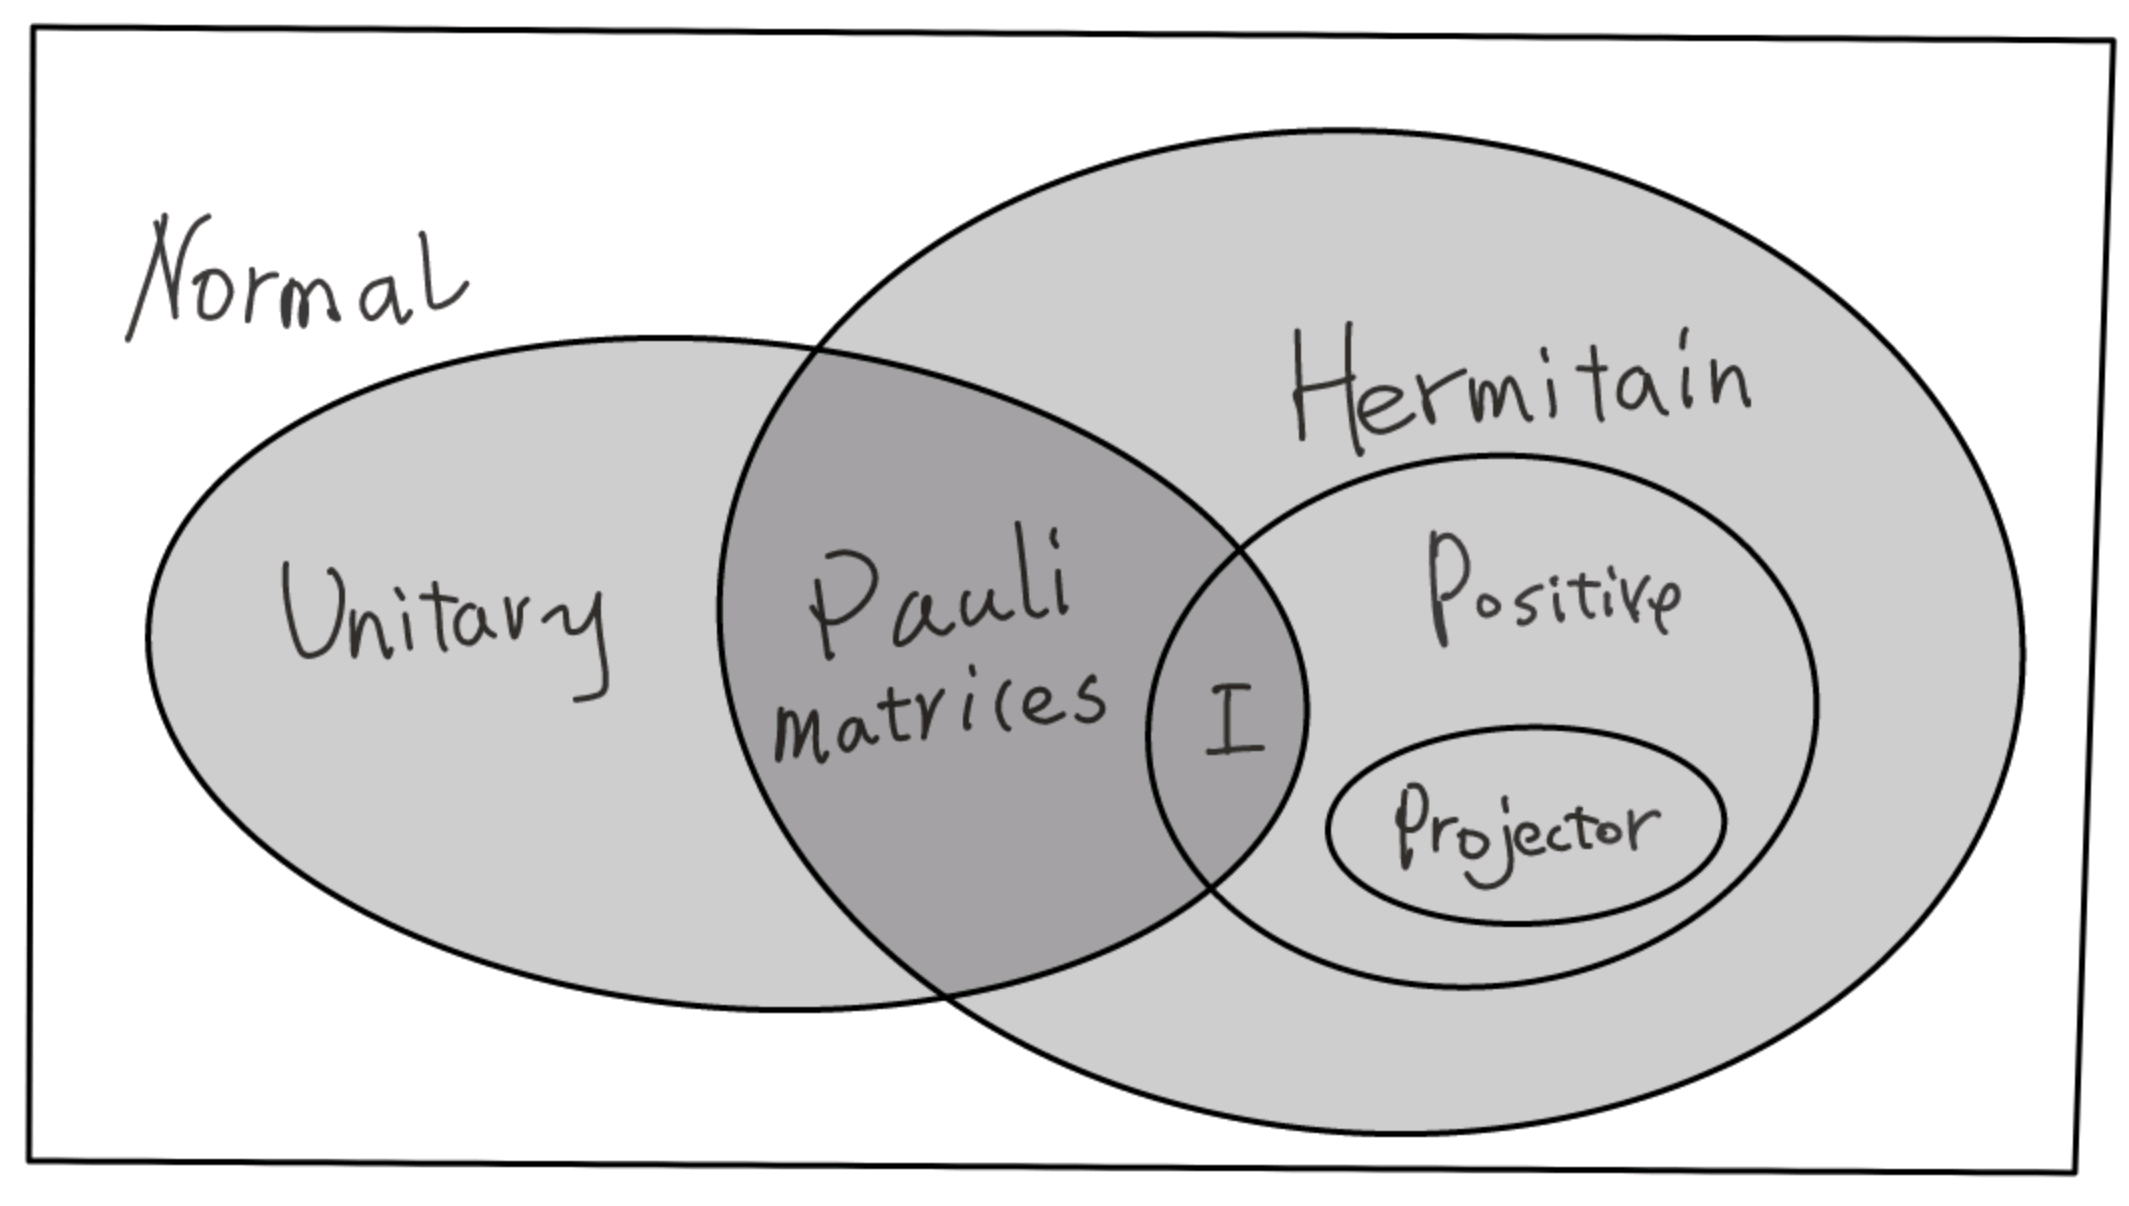
\includegraphics[width=0.75\linewidth]{Images/relations of many operators.png}
    \caption{\textbf{relations of many operators} }
\end{figure}
    % 2024-05-20 经LAI整理,已经初步完成

    \section{Tensor Products} 
    
\subsubsection{Tensor Product}

The tensor product is a way of putting vector spaces together to form larger vector spaces. 

% This construction is crucial to understanding the quantum mechanics of multiparticle systems. 

Suppose $V$ and $W$ are vector spaces of dimension $m$ and $n$ respectively. For convenience we also suppose that $V$ and $W$ are Hilbert spaces. 

Then $V \otimes W$ (read ' $V$ tensor $W^{\prime}$ ) is an $m n$ dimensional vector space. The elements of $V \otimes W$ are linear combinations of 'tensor products' $|v\rangle \otimes|w\rangle$ of elements $|v\rangle$ of $V$ and $|w\rangle$ of $W$.

In particular, if $|i\rangle$ and $|j\rangle$ are orthonormal bases for the spaces $V$ and $W$ then $|i\rangle \otimes|j\rangle$ is a basis for $V \otimes W$. 

We often use the abbreviated notations $|v\rangle|w\rangle,|v, w\rangle$ or even $|v w\rangle$ for the tensor product $|v\rangle \otimes|w\rangle$. 

\begin{example}
    For example, if $V$ is a two-dimensional vector space with basis vectors $|0\rangle$ and $|1\rangle$ then $|0\rangle \otimes|0\rangle+|1\rangle \otimes|1\rangle$ is an element of $V \otimes V$.
\end{example}

By definition the tensor product satisfies the following basic properties:
\begin{enumerate}
    \item For an arbitrary scalar $z$ and elements $|v\rangle$ of $V$ and $|w\rangle$ of $W$,
\begin{equation}
    z(|v\rangle \otimes|w\rangle)=(z|v\rangle) \otimes|w\rangle=|v\rangle \otimes(z|w\rangle)
\end{equation}
    \item For arbitrary $\left|v_{1}\right\rangle$ and $\left|v_{2}\right\rangle$ in $V$ and $|w\rangle$ in $W$,
\begin{equation}
    \left(\left|v_{1}\right\rangle+\left|v_{2}\right\rangle\right) \otimes|w\rangle=\left|v_{1}\right\rangle \otimes|w\rangle+\left|v_{2}\right\rangle \otimes|w\rangle .
\end{equation}
    \item For arbitrary $|v\rangle$ in $V$ and $\left|w_{1}\right\rangle$ and $\left|w_{2}\right\rangle$ in $W$,
\begin{equation}
    |v\rangle \otimes\left(\left|w_{1}\right\rangle+\left|w_{2}\right\rangle\right)=|v\rangle \otimes\left|w_{1}\right\rangle+|v\rangle \otimes\left|w_{2}\right\rangle .
\end{equation}
\end{enumerate}

The inner products on the spaces $V$ and $W$ can be used to define \textit{a natural inner product on $V \otimes W$}. Define
\begin{equation}
    \left(\sum_{i} a_{i}\left|v_{i}\right\rangle \otimes\left|w_{i}\right\rangle, \sum_{j} b_{j}\left|v_{j}^{\prime}\right\rangle \otimes\left|w_{j}^{\prime}\right\rangle\right) \equiv \sum_{i j} a_{i}^{*} b_{j}\left\langle v_{i} | v_{j}^{\prime}\right\rangle\left\langle w_{i} | w_{j}^{\prime}\right\rangle.
\end{equation}
It can be shown that the function so defined is a well-defined inner product. From this inner product, the inner product space $V \otimes W$ inherits the other structure we are familiar with, such as notions of an adjoint, unitarity, normality, and Hermiticity.

\subsubsection{Linear Operators $A \otimes B$ Act on the Space $V \otimes W$}

What sorts of linear operators act on the space $V \otimes W$ ? Suppose $|v\rangle$ and $|w\rangle$ are vectors in $V$ and $W$, and \textit{$A$ and $B$ are linear operators on $V$ and $W$}, respectively. Then we can define a linear operator $A \otimes B$ on $V \otimes W$ by the equation
\begin{equation}
    (A \otimes B)(|v\rangle \otimes|w\rangle) \equiv A|v\rangle \otimes B|w\rangle.
\end{equation}
The definition of $A \otimes B$ is then extended to all elements of $V \otimes W$ in the natural way to ensure linearity of $A \otimes B$, that is,
\begin{equation}
    (A \otimes B)\left(\sum_{i} a_{i} \left(\left|v_{i}\right\rangle \otimes\left|w_{i}\right\rangle\right) \right)  \equiv \sum_{i} a_{i} \left( A\left|v_{i}\right\rangle \otimes B\left|w_{i}\right\rangle \right) .
\end{equation}
It can be shown that $A \otimes B$ defined in this way is a well-defined linear operator on $V \otimes W$. 

This notion of the tensor product of two operators extends in the obvious way to the case where $A: V \rightarrow V^{\prime}$ and $B: W \rightarrow W^{\prime}$ map between different vector spaces. Indeed, an arbitrary linear operator $C$ mapping $V \otimes W$ to $V^{\prime} \otimes W^{\prime}$ can be represented as a linear combination of tensor products of operators mapping $V$ to $V^{\prime}$ and $W$ to $W^{\prime}$,
\begin{equation}
    C=\sum_{i} c_{i} A_{i} \otimes B_{i}
\end{equation}
where by definition
\begin{equation}
    \left(\sum_{i} c_{i} A_{i} \otimes B_{i}\right)|v\rangle \otimes|w\rangle \equiv \sum_{i} c_{i} A_{i}|v\rangle \otimes B_{i}|w\rangle .
\end{equation}

\subsubsection{Kronecker Product}

All this discussion is rather abstract. It can be made much more concrete by moving to a convenient matrix representation known as the Kronecker product. 

Suppose $A$ is an $m$ by $n$ matrix, and $B$ is a $p$ by $q$ matrix. Then we have the matrix representation:
\begin{equation}
    A \otimes B \equiv \overbrace{\left[\begin{array}{cccc}
A_{11} B & A_{12} B & \cdots & A_{1 n} B \\
A_{21} B & A_{22} B & \cdots & A_{2 n} B \\
\vdots & \vdots & \vdots & \vdots \\
A_{m 1} B & A_{m 2} B & \cdots & A_{m n} B
\end{array}\right]}^{n q}\} m p
\end{equation}

In this representation terms like $A_{11} B$ denote $p$ by $q$ submatrices whose entries are proportional to $B$, with overall proportionality constant $A_{11}$. For example, the tensor product of the vectors $(1,2)$ and $(2,3)$ is the vector
\begin{equation}
    \left[\begin{array}{l}
1 \\
2
\end{array}\right] \otimes\left[\begin{array}{l}
2 \\
3
\end{array}\right]=\left[\begin{array}{l}
1 \times 2 \\
1 \times 3 \\
2 \times 2 \\
2 \times 3
\end{array}\right]=\left[\begin{array}{l}
2 \\
3 \\
4 \\
6
\end{array}\right].
\end{equation}
The tensor product of the Pauli matrices $X$ and $Y$ is
\begin{equation}
    X \otimes Y=\left[\begin{array}{cc}
0 \cdot Y & 1 \cdot Y \\
1 \cdot Y & 0 \cdot Y
\end{array}\right]=\left[\begin{array}{cccc}
0 & 0 & 0 & -i \\
0 & 0 & i & 0 \\
0 & -i & 0 & 0 \\
i & 0 & 0 & 0
\end{array}\right].
\end{equation}

Finally, we mention the useful notation $|\psi\rangle^{\otimes k}$, which means $|\psi\rangle$ tensored with itself $k$ times. For example $|\psi\rangle^{\otimes 2}=|\psi\rangle \otimes|\psi\rangle$. An analogous notation is also used for operators on tensor product spaces.

Exercise 2.26: Let $|\psi\rangle=(|0\rangle+|1\rangle) / \sqrt{2}$. Write out $|\psi\rangle^{\otimes 2}$ and $|\psi\rangle^{\otimes 3}$ explicitly, both in terms of tensor products like $|0\rangle|1\rangle$, and using the Kronecker product.

Exercise 2.27: Calculate the matrix representation of the tensor products of the Pauli operators (a) $X$ and $Z$; (b) $I$ and $X$; (c) $X$ and $I$. Is the tensor product commutative? (No!)

% 下面的属性是重点!
Exercise 2.28: Show that the transpose, complex conjugation, and adjoint operations distribute over the tensor product,
\begin{equation}
    (A \otimes B)^{*}=A^{*} \otimes B^{*} ;(A \otimes B)^{T}=A^{T} \otimes B^{T} ;(A \otimes B)^{\dagger}=A^{\dagger} \otimes B^{\dagger} .
\end{equation}

Exercise 2.29: Show that the \textbf{tensor product of two unitary operators is unitary.}

Exercise 2.30: Show that the\textbf{ tensor product of two Hermitian operators is Hermitian.}

Exercise 2.31: Show that the\textbf{ tensor product of two positive operators is positive.}

Exercise 2.32: Show that the \textbf{tensor product of two projectors is a projector.}

Exercise 2.33: The Hadamard operator on one qubit may be written as
\begin{equation}
    H
=\frac{1}{\sqrt{2}}[(|0\rangle+|1\rangle)\langle 0|+(|0\rangle-|1\rangle)\langle 1|]
=\frac{1}{\sqrt{2}}[|0\rangle\langle 0|+| 0\rangle\langle 1|+| 1\rangle\langle 0|-| 1\rangle\langle 1|].
\end{equation}
Hence:
\begin{equation}
    H=\frac{1}{\sqrt{2}} \sum_{x, y}(-1)^{x \cdot y}|x\rangle\langle y|,
\end{equation}
where $x, y$ run over 0 and 1 .

Show explicitly that the Hadamard transform on $n$ qubits, $H^{\otimes n}$, may be written as
\begin{equation}
    H^{\otimes n}
=\frac{1}{\sqrt{2^n}} \sum_{\mathbf{x}, \mathbf{y}}(-1)^{\mathbf{x} \cdot \mathbf{y}}|\mathbf{x}\rangle\langle\mathbf{y}|,
\end{equation}
where $\mathbf{x}, \mathbf{y}$ are length $n$-binary strings. $\mathbf{x} \cdot \mathbf{y}$ is inner product of that two strings.

Now explicitly writing $H^{\otimes 2}$, we have:
\begin{equation}
\begin{aligned}
H^{\otimes 2} & =\frac{1}{\sqrt{2^2}} \sum_{\mathbf{x}, \mathbf{y}}(-1)^{(\mathbf{x} \cdot \mathbf{y})}|\mathbf{x}\rangle\langle\mathbf{y}| \\
& \cong \frac{1}{2}\left[\begin{array}{cccc}
1 & 1 & 1 & 1 \\
1 & -1 & 1 & -1 \\
1 & 1 & -1 & -1 \\
1 & -1 & -1 & 1
\end{array}\right]
\end{aligned}
\end{equation}

Note that here, $\mathbf{x}, \mathbf{y}$ are binary length 2 strings. The sum goes through all pairwise combinations of $\mathbf{x}, \mathbf{y} \in\{00,01,10,11\}$
    % 2024-05-20 经LAI整理,已经初步完成

    \section{Operator Functions} 
    
There are many important functions which can be defined for operators and matrices. 

\subsubsection{Operator Functions}

Let $A=\sum_{a} a|a\rangle\langle a|$ be a spectral decomposition for a normal operator $A$. Is this decomposition form unique for the normal operator $A$? Actually, if there is an eigenspace is more than one dimensional, that is, there are more than one orthonormal eigenvectors sharing the same eigenvalue (in this case, we say $A$ is \textit{degenerate}); then, the spectral decomposition of $A$ is not unique (For more detail, see \href{https://physics.stackexchange.com/questions/576287/uniqueness-of-spectral-decomposition}{here}). But the eigenspaces corresponding to each eigenvalue are fixed. We can consider the unique spectral decomposition by using the notations of projectors of eigenspaces as following. Let 
\begin{equation}
    A=\sum_{a} a P_{a}
\end{equation}
be a spectral decomposition for a normal operator $A$, where all numbers $a$'s over the sum are distinct, and operator $P_{a}$ denotes the projector of eigenspace $V_a$ of $a.$ If $\dim V_a =d$, then we can construct projector $P_a:= \sum_{i=1}^{d} |a_{i}\rangle\langle a_{i}|$. We can show that the projector $P_a$ is invariant under the choosing arbitrary orthonormal basis $|a_{i}\rangle$ of eigenspace $V_a$. (To see the invariability, You can refer to the Lemma 2.1.3 in Zhijian Lai's master thesis at \href{https://galvinlai.github.io/files/doc/master_thesis_2021.pdf}{here}.)

Now we are ready to define the operator functions, or say, matrix function as below.

Given a function $f$ from the complex numbers to the complex numbers, it is possible to define a corresponding \textit{matrix function} on the set of normal matrices (or some subclass, such as the vector space of Hermitian matrices) by the following construction. 

Let $A=\sum_{a} a|a\rangle\langle a|$ be a spectral decomposition for a normal operator $A$. Define 
\begin{equation}
    f(A) \equiv \sum_{a} f(a)|a\rangle\langle a|.
\end{equation}
A little thought shows that $f(A)$ is uniquely defined. Because, we can rewrite the decomposition as$A=\sum_{a} a P_{a}$, then 
\begin{equation}
    f(A) \equiv \sum_{a} f(a) P_{a}
\end{equation}
where the numbers $f(a)$ and projectors $P_{a}$ are uniquely determined by $A$ itself, instead of the choose of orthogonal basis $|a\rangle$ of $V.$ This procedure can be used, for example, to define 
\begin{itemize}
    \item the square root of a positive operator $A$ (whose all eigenvalues are non-negative):
\begin{equation}
    \sqrt{A} \equiv \sum_{a} \sqrt{a} |a\rangle\langle a|.
\end{equation}
    \item the logarithm of a positive-definite operator $A$ (whose all eigenvalues are positive):
\begin{equation}
    \log (A) \equiv \sum_{a} \log (a)|a\rangle\langle a|.
\end{equation}
    \item the exponential of a normal operator $A$ . 
\begin{equation}
    \exp (A) \equiv \sum_{a} \exp (a)|a\rangle\langle a|.
\end{equation}
\end{itemize}
In general, we often define the matrix exponential for any square matrices $A$ (not necessarily to be normal) as
\begin{equation}
    \exp (A) =\sum_{k=0}^{\infty} \frac{1}{k!} A^k.
\end{equation}
Indeed, for the normal matrix, the two definition are equivalent. Let $A=\sum_{a} a|a\rangle\langle a|$ be a spectral decomposition for a normal operator $A$. Then,
\begin{align}
    A^2
    &=\left(  \sum_{a} a|a\rangle\langle a| \right)\left(  \sum_{a^{\prime}} a^{\prime}|a^{\prime}\rangle\langle a^{\prime}| \right) \\
    &= \sum_{a}  \sum_{a^{\prime}}  a a^{\prime}|a\rangle\langle a|a^{\prime}\rangle\langle a^{\prime}| \\
    &=\sum_{a} a^2|a\rangle\langle a|.
\end{align}
Similarly, we have $A^k=\sum_{a} a^k|a\rangle\langle a|$. Then, we have
\begin{align}
\exp (A) 
&=\sum_{k=0}^{\infty} \frac{1}{k!} A^k \\
&=\sum_{k=0}^{\infty} \frac{1}{k!}  \left(\sum_{a} a^k|a\rangle\langle a|\right)\\
&=\sum_{a} \left( \sum_{k=0}^{\infty} \frac{1}{k!}  a^k \right)|a\rangle\langle a|\\
&=\sum_{a} \exp (a)|a\rangle\langle a|.
\end{align}
See \href{https://en.wikipedia.org/wiki/Matrix_exponential}{wiki} for more nice properties of matrix exponential function. If a matrix is diagonal:
\begin{equation}
    A=\left[\begin{array}{cccc}
a_1 & 0 & \cdots & 0 \\
0 & a_2 & \cdots & 0 \\
\vdots & \vdots & \ddots & \vdots \\
0 & 0 & \cdots & a_n
\end{array}\right],
\end{equation}
then its exponential can be obtained by exponentiating each entry on the main diagonal:
\begin{equation}
    e^A=\left[\begin{array}{cccc}
e^{a_1} & 0 & \cdots & 0 \\
0 & e^{a_2} & \cdots & 0 \\
\vdots & \vdots & \ddots & \vdots \\
0 & 0 & & a_n
\end{array}\right] .
\end{equation}
As an example,
\begin{equation}
    \exp (\theta Z)=\left[\begin{array}{cc}
e^{\theta} & 0 \\
0 & e^{-\theta}
\end{array}\right].
\end{equation}
In the other hand, we obtain the same result by definition $\exp (A) \equiv \sum_{a} \exp (a)|a\rangle\langle a|.$

\begin{exercise}
Exercise 2.34: Find the square root and logarithm of the matrix
\begin{equation}
    \left[\begin{array}{ll}
4 & 3 \\
3 & 4
\end{array}\right]
\end{equation}
\end{exercise}

\begin{exercise}
Exercise 2.35: (Exponential of the Pauli matrices) Let $\vec{v}$ be any real, three-dimensional unit vector and $\theta$ a real number. Prove that
\begin{equation}
    \exp (i \theta \vec{v} \cdot \vec{\sigma})=\cos (\theta) I+i \sin (\theta) \vec{v} \cdot \vec{\sigma}
\end{equation}

where $\vec{v} \cdot \vec{\sigma} \equiv \sum_{i=1}^{3} v_{i} \sigma_{i}$. This exercise is generalized in Problem 2.1 on page 117.
\end{exercise}

\subsubsection{Trace}

The trace of a squared matrix $A$ is defined to be the sum of its diagonal elements,
\begin{equation}
    \operatorname{tr}(A) \equiv \sum_{i} A_{i i}.
\end{equation}
The trace is easily seen to be \textit{cyclic}, $\operatorname{tr}(A B)=\operatorname{tr}(B A)$, and linear, $\operatorname{tr}(A+B)=\operatorname{tr}(A)+\operatorname{tr}(B), \operatorname{tr}(z A)=z \operatorname{tr}(A)$, where $A$ and $B$ are arbitrary matrices, and $z$ is a complex number. 

Furthermore, from the cyclic property it follows that the trace of a matrix is invariant under the \textit{unitary similarity transformation} 
\begin{equation}
    A \rightarrow U A U^{\dagger},
\end{equation}
as $\operatorname{tr}\left(U A U^{\dagger}\right)=$ $\operatorname{tr}\left(U^{\dagger} U A\right)=\operatorname{tr}(A)$. In light of this result, it makes sense to define the \textit{trace of an operator $A$} to be the trace of any matrix representation of $A$.

As an example of the trace, suppose $|\psi\rangle$ is a unit vector and $A$ is an arbitrary operator. To evaluate $\operatorname{tr}(A|\psi\rangle\langle\psi|)$, use the Gram-Schmidt procedure to extend $|\psi\rangle$ to an orthonormal basis $|i\rangle$ which includes $|\psi\rangle$ as the first element. Then we have
\begin{equation}
\begin{aligned}
\operatorname{tr}(A|\psi\rangle\langle\psi|) 
& =\sum_{i}\langle i| \left(A| \psi\rangle\langle\psi | \right) | i\rangle \\
& =\sum_{i}\langle i| A| \psi\rangle\langle\psi |  i\rangle \\
& =\sum_{i}\left(\langle\psi |  i\rangle\langle i| \right) A| \psi\rangle \\
& =\langle\psi|A| \psi\rangle.
\end{aligned}
\end{equation}
This result, that 
\begin{equation}
    \operatorname{tr}(A|\psi\rangle\langle\psi|)=\langle\psi|A| \psi\rangle
\end{equation}
is extremely useful in evaluating the trace of an operator. Again, this result directly comes from the cyclic property of the trace.

\begin{exercise}
Exercise 2.36: Show that the Pauli matrices except for $I$ have trace zero.
\end{exercise}

\begin{exercise}
Exercise 2.37: (Cyclic property of the trace) If $A$ and $B$ are two linear operators show that $\operatorname{tr}(A B)=\operatorname{tr}(B A).$
\end{exercise}

\begin{exercise}
Exercise 2.38: (Linearity of the trace) If $A$ and $B$ are two linear operators, show that $\operatorname{tr}(A+B)=\operatorname{tr}(A)+\operatorname{tr}(B)$ and if $z$ is an arbitrary complex number show that $\operatorname{tr}(z A)=z \operatorname{tr}(A)$.
\end{exercise}

\begin{exercise}
Exercise 2.39: (The Hilbert-Schmidt inner product on operators) The set $L_{V}$ of linear operators on a Hilbert space $V$ is obviously a vector space over $\mathbb{C}$- the sum of two linear operators is a linear operator, $z A$ is a linear operator if $A$ is a linear operator and $z$ is a complex number, and there is a zero element 0 . 

An important additional result is that the vector space $L_{V}$ can be given a natural inner product structure, turning it into a Hilbert space.
\begin{enumerate}
    \item Show that the function $(\cdot, \cdot)$ on $L_{V} \times L_{V}$ defined by
\begin{equation}
    (A, B) \equiv \operatorname{tr}\left(A^{\dagger} B\right)
\end{equation}
is an inner product function. This inner product is known as the Hilbert-Schmidt or trace inner product.
    \item If $V$ has $d$ dimensions show that $L_{V}$ has dimension $d^{2}$.
    \item Find an orthonormal basis of Hermitian matrices for the Hilbert space $L_{V}$.
\end{enumerate}
\end{exercise}
    % 2024-05-20 经LAI整理,已经初步完成

    \section{The Commutator and Anti-commutator} 
    The \textit{commutator} between two operators $A$ and $B$ is defined to be
\begin{equation}
    [A, B] \equiv A B-B A.
\end{equation}
If $[A, B]=0$, that is, $A B=B A$, then we say $A$ commutes with $B$. 

Similarly, the \textit{anti-commutator} of two operators $A$ and $B$ is defined by
\begin{equation}
    \{A, B\} \equiv A B+B A.
\end{equation}
We say $A$ anti-commutes with $B$ if $\{A, B\}=0$. 

% It turns out that many important properties of pairs of operators can be deduced from their commutator and anti-commutator.

Perhaps the most useful relation is the following connection between the commutator and the property of being able to \textit{simultaneously diagonalize} Hermitian operators $A$ and $B$, that is, write 
\begin{equation}
    A=\sum_{i} a_{i}|i\rangle\langle i|, B=\sum_{i} b_{i}| i\rangle\langle i|
\end{equation}
where $|i\rangle$ is some common orthonormal set of eigenvectors for $A$ and $B$.

\begin{theorem}
    Theorem 2.2: (\textbf{Simultaneous} diagonalization theorem) Suppose $A$ and $B$ are Hermitian operators. Then $[A, B]=0$ if and only if there exists an orthonormal basis such that both $A$ and $B$ are diagonal with respect to that basis. We say that $A$ and $B$ are simultaneously diagonalizable in this case.
\end{theorem}

This result connects the commutator of two operators, which is often easy to compute, to the property of being simultaneously diagonalizable, which is a prior rather difficult to determine. As an example, consider that
\begin{equation}
\begin{aligned}
{[X, Y] } & =\left[\begin{array}{ll}
0 & 1 \\
1 & 0
\end{array}\right]\left[\begin{array}{rr}
0 & -i \\
i & 0
\end{array}\right]-\left[\begin{array}{rr}
0 & -i \\
i & 0
\end{array}\right]\left[\begin{array}{ll}
0 & 1 \\
1 & 0
\end{array}\right] \\
& =2 i\left[\begin{array}{rr}
1 & 0 \\
0 & -1
\end{array}\right] \\
& =2 i Z
\end{aligned}
\end{equation}
so $X$ and $Y$ do not commute. You have already shown, in Exercise 2.11, that $X$ and $Y$ do not have common eigenvectors, as we expect from the simultaneous diagonalization theorem.

\begin{proof}
    You can (and should!) easily verify that if $A$ and $B$ are diagonal in the same orthonormal basis then $[A, B]=0$. To show the converse, let $|a, j\rangle$ be an orthonormal basis for the eigenspace $V_{a}$ of $A$ with eigenvalue $a$; the index $j$ is used to label possible degeneracies. Note that
\begin{equation}
    A B|a, j\rangle=B A|a, j\rangle=a B|a, j\rangle
\end{equation}
and therefore $B|a, j\rangle$ is an element of the eigenspace $V_{a}$. Let $P_{a}$ denote the projector onto the space $V_{a}$ and define $B_{a} \equiv P_{a} B P_{a}$. It is easy to see that the restriction of $B_{a}$ to the space $V_{a}$ is Hermitian on $V_{a}$, and therefore has a spectral decomposition in terms of an orthonormal set of eigenvectors which span the space $V_{a}$. Let's call these eigenvectors $|a, b, k\rangle$, where the indices $a$ and $b$ label the eigenvalues of $A$ and $B_{a}$, and $k$ is an extra index to allow for the possibility of a degenerate $B_{a}$. Note that $B|a, b, k\rangle$ is an element of $V_{a}$, so $B|a, b, k\rangle=P_{a} B|a, b, k\rangle$. Moreover we have $P_{a}|a, b, k\rangle=|a, b, k\rangle$, so
\begin{equation}
    B|a, b, k\rangle=P_{a} B P_{a}|a, b, k\rangle=b|a, b, k\rangle .
\end{equation}
It follows that $|a, b, k\rangle$ is an eigenvector of $B$ with eigenvalue $b$, and therefore $|a, b, k\rangle$ is an orthonormal set of eigenvectors of both $A$ and $B$, spanning the entire vector space on which $A$ and $B$ are defined. That is, $A$ and $B$ are simultaneously diagonalizable.
\end{proof}

\begin{exercise}
Exercise 2.40: (Commutation relations for the Pauli matrices) Verify the commutation relations
\begin{equation}
    [X, Y]=2 i Z ; \quad[Y, Z]=2 i X ; \quad[Z, X]=2 i Y .
\end{equation}
There is an elegant way of writing this using $\epsilon_{j k l}$, the anti-symmetric tensor on three indices, for which $\epsilon_{j k l}=0$ except for $\epsilon_{123}=\epsilon_{231}=\epsilon_{312}=1$, and $\epsilon_{321}=\epsilon_{213}=\epsilon_{132}=-1:$
\begin{equation}
    \left[\sigma_{j}, \sigma_{k}\right]=2 i \sum_{l=1}^{3} \epsilon_{j k l} \sigma_{l}
\end{equation}
\end{exercise}

\begin{exercise}
Exercise 2.41: (Anti-commutation relations for the Pauli matrices) Verify the anti-commutation relations
\begin{equation}
    \left\{\sigma_{i}, \sigma_{j}\right\}=0
\end{equation}
where $i \neq j$ are both chosen from the set $1,2,3$. Also verify that $(i=0,1,2,3)$
\begin{equation}
    \sigma_{i}^{2}=I
\end{equation}
\end{exercise}

\begin{exercise}
Exercise 2.42: Verify that
\begin{equation}
    A B=\frac{[A, B]+\{A, B\}}{2}.
\end{equation}
\end{exercise}

\begin{exercise}
Exercise 2.43: Show that for $j, k=1,2,3$,
\begin{equation}
    \sigma_{j} \sigma_{k}=\delta_{j k} I+i \sum_{l=1}^{3} \epsilon_{j k l} \sigma_{l}.
\end{equation}
\end{exercise}

\begin{exercise}
Exercise 2.44: Suppose $[A, B]=0,\{A, B\}=0$, and $A$ is invertible. Show that $B$ must be 0 .
\end{exercise}

\begin{exercise}
Exercise 2.45: Show that $[A, B]^{\dagger}=\left[B^{\dagger}, A^{\dagger}\right]$. Compared to $\{A, B\}^{\dagger}=\{A^{\dagger}, B^{\dagger}\}$.
\end{exercise}

\begin{exercise}
Exercise 2.46: Show that $[A, B]=-[B, A]$. Compared to $\{A, B\}=\{B, A\}$.
\end{exercise}

\begin{exercise}
Exercise 2.47: Suppose $A$ and $B$ are Hermitian. Show that $i[A, B]$ is Hermitian.
\end{exercise}
    % 2024-05-20 经LAI整理,已经初步完成

    \section{The Polar and Singular Value Decomposition} 
    The polar and singular value decompositions are useful ways of breaking linear operators up into simpler parts. In particular, these decompositions allow us to break general linear operators up into products of unitary operators and positive operators. 

% While we don't understand the structure of general linear operators terribly well, we do understand unitary operators and positive operators in quite some detail. The polar and singular value decompositions allow us to apply this understanding to better understand general linear operators.

\begin{theorem}
Theorem 2.3: (Polar decomposition) Let $A$ be a linear operator on a vector space $V$. Then there exists unitary $U$ and positive operators $J$ and $K$ such that
\begin{equation}
    A=U J=K U
\end{equation}
where the unique positive operators $J$ and $K$ satisfying these equations are defined by $J \equiv \sqrt{A^{\dagger} A}$ and $K \equiv \sqrt{A A^{\dagger}}$. Moreover, if $A$ is invertible then $U$ is unique.
\end{theorem}

We call the expression $A=U J$ the left polar decomposition of $A$, and $A=K U$ the right polar decomposition of $A$. Most often, we'll omit the 'right' or 'left' nomenclature, and use the term 'polar decomposition' for both expressions, with context indicating which is meant.

\begin{proof}
    $J \equiv \sqrt{A^{\dagger} A}$ is a positive operator, so it can be given a spectral decomposition, $J=$ $\sum_{i} \lambda_{i}|i\rangle\langle i|\left(\lambda_{i} \geq 0\right)$. Define $\left|\psi_{i}\right\rangle \equiv A|i\rangle$. From the definition, we see that $\left\langle\psi_{i} | \psi_{i}\right\rangle=\lambda_{i}^{2}$. Consider for now only those $i$ for which $\lambda_{i} \neq 0$. For those $i$ define $\left|e_{i}\right\rangle \equiv\left|\psi_{i}\right\rangle / \lambda_{i}$, so the $\left|e_{i}\right\rangle$ are normalized. Moreover, they are orthogonal, since if $i \neq j$ then $\left\langle e_{i} | e_{j}\right\rangle=$ $\left\langle i\left|A^{\dagger} A\right| j\right\rangle / \lambda_{i} \lambda_{j}=\left\langle i\left|J^{2}\right| j\right\rangle / \lambda_{i} \lambda_{j}=0$

We have been considering $i$ such that $\lambda_{i} \neq 0$. Now use the Gram-Schmidt procedure to extend the orthonormal set $\left|e_{i}\right\rangle$ so it forms an orthonormal basis, which we also label $\left|e_{i}\right\rangle$. Define a unitary operator $U \equiv \sum_{i}\left|e_{i}\right\rangle\langle i|$. When $\lambda_{i} \neq 0$ we have $U J|i\rangle=\lambda_{i}\left|e_{i}\right\rangle=$ $\left|\psi_{i}\right\rangle=A|i\rangle$. When $\lambda_{i}=0$ we have $U J|i\rangle=0=\left|\psi_{i}\right\rangle$. We have proved that the action of $A$ and $U J$ agree on the basis $|i\rangle$, and thus that $A=U J$.

$J$ is unique, since multiplying $A=U J$ on the left by the adjoint equation $A^{\dagger}=J U^{\dagger}$ gives $J^{2}=A^{\dagger} A$, from which we see that $J=\sqrt{A^{\dagger} A}$, uniquely. A little thought shows that if $A$ is invertible, then so is $J$, so $U$ is uniquely determined by the equation $U=A J^{-1}$. The proof of the right polar decomposition follows, since $A=U J=U J U^{\dagger} U=K U$, where $K \equiv U J U^{\dagger}$ is a positive operator. Since $A A^{\dagger}=K U U^{\dagger} K=K^{2}$ we must have $K=\sqrt{A A^{\dagger}}$, as claimed.
\end{proof}

The singular value decomposition combines the polar decomposition and the spectral theorem.

\begin{corollary}
Corollary 2.4: (Singular value decomposition) Let $A$ be a square matrix. Then there exist unitary matrices $U$ and $V$, and a diagonal matrix $D$ with non-negative entries such that
\begin{equation}
    A=U D V
\end{equation}
The diagonal elements of $D$ are called the singular values of $A$.
\end{corollary}

\begin{proof}
    By the polar decomposition, $A=S J$, for unitary $S$, and positive $J$. By the spectral theorem, $J=T D T^{\dagger}$, for unitary $T$ and diagonal $D$ with non-negative entries. Setting $U \equiv S T$ and $V \equiv T^{\dagger}$ completes the proof.
\end{proof}

\begin{exercise}
Exercise 2.48: What is the polar decomposition of a positive matrix $P$? Of a unitary matrix $U$ ? Of a Hermitian matrix, $H$ ?
\end{exercise}

\begin{exercise}
Exercise 2.49: Express the polar decomposition of a normal matrix in the outer product representation.
\end{exercise}

\begin{exercise}
Exercise 2.50: Find the left and right polar decompositions of the matrix

\begin{equation}
    \left[\begin{array}{ll}
1 & 0 \\
1 & 1
\end{array}\right]
\end{equation}
\end{exercise}
    % 2024-05-20 经LAI整理,已经初步完成

\chapter{Other Mathematical Preliminaries}
% 本章内容是额外的数学基础知识,但并未在NCBOOK中被详细展开或者提及。

    \section{The Space of Hermitian Matrices} 
    \paragraph{Hermitian Matrices form a real Vector Space (only on real numbers)}

\begin{theorem}
    $H_n(\mathbb{C})$, the set of $n \times n$ Hermitian (complex-entry) matrices, forms a vector space over $\mathbb{R}$ with dimension $n^2$. Specially, it cannot be a vector space over $\mathbb{C}.$
\end{theorem}

\begin{remark}
   In contract, $M_n(\mathbb{C})$, the set of $n \times n$ (complex-entry) matrices, forms a vector space over $\mathbb{C}$ with dimension $n^2$.
\end{remark}

\subparagraph{\href{https://math.stackexchange.com/questions/1630604/show-that-the-set-of-hermitian-matrices-forms-a-real-vector-space}{linear algebra - Show that the set of Hermitian matrices forms a real vector space - Mathematics Stack Exchange} 
}
I give you the intuition for $2 \times 2$ matrices that you can extend to the general case.
An Hermitian $2 \times 2$ matrix has the form:
$$
\left[\begin{array}{ll}
a & b \\
\bar{b} & c
\end{array}\right]
$$
with: $a, c \in \mathbb{R}$ and $b \in \mathbb{C}$ ($\bar{b}$ is the complex conjugate of $b)$.

Now you can see that, for two matrices of this form, we have:
$$
\left[\begin{array}{ll}
a & b \\
\bar{b} & c
\end{array}\right]+\left[\begin{array}{ll}
x & y \\
\bar{y} & z
\end{array}\right]=\left[\begin{array}{ll}
a+x & b+y \\
\bar{b}+\bar{y} & c+z
\end{array}\right]
$$
and, since $\bar{b}+\bar{y}=\overline{b+y}$ the result is a matrix of the same form, i.e. an Hermitian matrix.

For the product we have:
$$
k\left[\begin{array}{ll}
a & b \\
\bar{b} & c
\end{array}\right]=\left[\begin{array}{ll}
k a & k b \\
k \bar{b} & k c
\end{array}\right]
$$
\textbf{so the result matrix is Hermitian only if $k$ is a real number}. Finally we see that the zero matrix is hermitian and the opposite of an Hermitian matrix is Hermitian, so th set of hermitian matrix is real vector space.

For the basis: Note that an hermitian matrix can be expressed as a linear combination with real coefficients in the form:
$$
\left[\begin{array}{ll}
a & b \\
\bar{b} & c
\end{array}\right]=a\left[\begin{array}{ll}
1 & 0 \\
0 & 0
\end{array}\right]+\operatorname{Re}(b)\left[\begin{array}{ll}
0 & 1 \\
1 & 0
\end{array}\right]+\operatorname{Im}(b)\left[\begin{array}{cc}
0 & i \\
-i & 0
\end{array}\right]+c\left[\begin{array}{ll}
0 & 0 \\
0 & 1
\end{array}\right]
$$
and ,since the four matrices at the right are linearly independent, these form a basis. 

\begin{example}
    Observe that
$$
i\left(\begin{array}{cc}
0 & i \\
-i & 0
\end{array}\right)+\left(\begin{array}{cc}
0 & 1 \\
1 & 0
\end{array}\right)=\left(\begin{array}{cc}
0 & 0 \\
2 & 0
\end{array}\right)
$$
is a $\mathbb{C}$-linear combination of Hermitian matrices, and the result is not Hermitian.
\end{example}


\subparagraph{\href{https://math.stackexchange.com/questions/2840794/what-is-dimension-over-mathbb-r-of-the-space-of-n-times-n-hermitian-matrice}{linear algebra - What is dimension over \$\mathbb R\$ of the space of \$n\textbackslash{}times n\$ Hermitian matrices? - Mathematics Stack Exchange} 
}
I believe the best way to approach such a problem is to try come up with a basis for the vector space.

The diagonal elements of such a matrix must be real in order to be equal to their complex conjugate. So the diagonal Hermitian matrices are spanned by the $n$ vectors
$$
\left(\begin{array}{lll}
1 & & \\
& \ldots & \\
& & 0
\end{array}\right),\left(\begin{array}{ccc}
0 & & \\
& \ldots & \\
& & 1
\end{array}\right) \text {. }
$$

Every other entry below the diagonal is the complex conjugate of the corresponding element above the diagonal, so the matrix is determined by the rest of the elements above the diagonal. Over $\mathbb{R}$, the basis for $\mathbb{C}$ is simply the vectors 1 and $i$. So there are two basis matrices for every position above the diagonal: the matrix which contains a 1 at position $(j, k)$ and the matrix which contains an $i$ at position $(j, k)$.

This yields $n+\sum_{k=1}^{n-1} 2 k=n+2 \frac{n(n-1)}{2}=n^2$
    % NCBOOK中未说明,但必须要懂得的基本常识

    \section{Partial Trace} 
    % 主要参考wiki
% \href{https://en.wikipedia.org/wiki/Partial_trace}{Partial trace - Wikipedia}

In linear algebra and functional analysis, the partial trace is a generalization of the trace. 
Whereas the trace is a scalar valued function on operators, the partial trace is an operator-valued function.

Suppose $V, W$ are finite-dimensional vector spaces over a field, with dimensions $m$ and $n$, respectively. 
For any vector space $A$, let $L(A)$ denote the space of linear operators on $A$.

\begin{definition}[partial trace I]\label{defn:partial-trace-1}
The \textbf{partial trace over $W$} is an operator-valued function written as
$$
\operatorname{Tr}_W: \mathrm{L}(V \otimes W) \rightarrow \mathrm{L}(V),
$$
where $\otimes$ denotes the tensor product. It is defined as follows: Let $e_1, \ldots, e_m$, and $f_1, \ldots, f_n$, be bases for $V$ and $W$ respectively; then $T \in \mathrm{L}(V \otimes W)$ has a matrix representation
$$
a_{k \ell, i j}, \quad 1 \leq k, i \leq m, \quad 1 \leq \ell, j \leq n
$$
relative to the basis $e_k \otimes f_{\ell}$ of $V \otimes W$. Now fix indices $k, i$ in the range $1, \ldots, m$, consider the sum
$$
b_{k, i}=\sum_{j=1}^n a_{k j, i j}
$$
This gives a matrix $b_{k, i}$. The associated linear operator (of matrix $b_{k, i}$) on \textit{V} is independent of the choice of bases and is by definition the partial trace.
\end{definition}

Among physicists, this is often called \textbf{"tracing out" or "tracing over" $W$} to leave only an operator on $V$ in the context where $W$ and $V$ are Hilbert spaces associated with quantum systems (see below).

The partial trace operator can be defined invariantly (that is, without reference to a basis) as follows.

\begin{definition}[partial trace II]
The \textbf{partial trace over $W$} is the unique linear map
$$
\operatorname{Tr}_W: \mathrm{L}(V \otimes W) \rightarrow \mathrm{L}(V)
$$
such that
\begin{equation}\label{eq:partial-trace-defn}
    \operatorname{Tr}_W(R \otimes S)=\operatorname{Tr}(S) R, \quad \forall R \in \mathrm{L}(V) \quad \forall S \in \mathrm{L}(W),
\end{equation}
where $\operatorname{Tr}(\cdot)$ is the usual trace of a linear operator.
\end{definition}

\begin{proof} % lai's proof
Definition \ref{defn:partial-trace-1} showed such linear map exists.
To see that the conditions (\ref{eq:partial-trace-defn}) determine the partial trace uniquely:
\begin{itemize}
  \item let $v_1, \ldots, v_m$ form an orthonormal basis for $V$ and let $w_1, \ldots, w_n$ form an orthonormal for $W$;
  \item let $E_{i j}: V \rightarrow V$ be the map that sends $v_i$ to $v_j$ (and all other basis elements to zero), then the maps $E_{i j}$ form a basis for $\mathrm{L}(V)$.
  \item let $F_{k l}: W \rightarrow W$ be the map that sends $w_k$ to $w_l$ (and all other basis elements to zero), then the maps $F_{k l}$ form a basis for $\mathrm{L}(W)$.
  \item we have $\operatorname{Tr}(E_{ij})=\operatorname{Tr}(F_{kl})=1.$
  \item since the vectors $v_i \otimes w_k$ form a basis for $V \otimes W$, the maps $E_{i j} \otimes F_{k l}$ form a basis for $\mathrm{L}(V \otimes W)$.
  \item for given \textit{any} partial trace $\operatorname{Tr}_W$, we always have that
\end{itemize}
$$
\operatorname{Tr}_W(E_{i j} \otimes F_{k l})=\operatorname{Tr}(F_{k l}) E_{i j} = E_{i j}.
$$
\end{proof}

From this abstract definition, the following properties follow:

\begin{proposition}
$$
\begin{aligned}
& \operatorname{Tr}_W\left(T\left(I_V \otimes S\right)\right)=\operatorname{Tr}_W\left(\left(I_V \otimes S\right) T\right) ,\quad \forall S \in \mathrm{L}(W) \quad \forall T \in \mathrm{L}(V \otimes W).
\end{aligned}
$$
\end{proposition}

\begin{proof}
    my proof is done on
\end{proof}

The partial trace can be viewed as a quantum operation.

Consider a quantum mechanical system whose state space is the tensor product $H_A \otimes H_B$ of Hilbert spaces. A mixed state is described by a density matrix $\rho$, that is a non-negative trace-class operator of trace 1 on the tensor product $H_A \otimes H_B$. The partial trace of $\rho$ with respect to the system $B$, denoted by $\rho^A$, is called the reduced state of $\rho$ on system $A$. In symbols,
$$
\rho^A=\operatorname{Tr}_B \rho
$$

To show that this is indeed a sensible way to assign a state on the $A$ subsystem to $\rho$, we offer the following justification. 

Let $M$ be an observable on the subsystem $A$, then the corresponding observable on the composite system is $M \otimes I$. However one chooses to define a reduced state $\rho^A$, there should be consistency of measurement statistics. The expectation value of $M$ after the subsystem $A$ is prepared in $\rho^A$ and that of $M \otimes I$ when the composite system is prepared in $\rho$ should be the same, i.e. the following equality should hold:
$$
\operatorname{Tr}\left(M \cdot \rho^A\right)=\operatorname{Tr}(M \otimes I \cdot \rho) .
$$
We see that this is satisfied if $\rho^A$ is as defined above via the partial trace. Furthermore, such operation is unique.

\begin{proof}
    my proof is done on
\end{proof}
    % 2024-05-20 经LAI整理,已经初步完成

    \section{Discrete Fourier Transform} 
    
\href{https://en.wikipedia.org/wiki/Discrete_Fourier_transform}{Discrete Fourier transform - Wikipedia}

\begin{definition}
The \textbf{discrete Fourier transform (DFT)} transforms a sequence of $N$ complex numbers $\left\{\mathbf{x}_n\right\}:=x_0, x_1, \ldots, x_{N-1}$ into another sequence of complex numbers, $\left\{\mathbf{X}_k\right\}:=X_0, X_1, \ldots, X_{N-1}$, which is defined by:
$$
X_k=\sum_{n=0}^{N-1} x_n \cdot e^{-i 2 \pi \frac{k}{N} n}
$$
The transform is sometimes denoted by the symbol $\mathcal{F}$, as in $\mathbf{X}=\mathcal{F}\{\mathbf{x}\}$ or $\mathcal{F}(\mathbf{x})$ or $\mathcal{F} \mathbf{x}$.
\end{definition}

The inverse transform is given by:
$$
x_n=\frac{1}{N} \sum_{k=0}^{N-1} X_k \cdot e^{i 2 \pi \frac{k}{N} n}
$$

\begin{example}
    This example demonstrates how to apply the DFT to a sequence of length $N=4$ and the input vector
$$
\mathbf{x}=\left(\begin{array}{l}
x_0 \\
x_1 \\
x_2 \\
x_3
\end{array}\right)=\left(\begin{array}{c}
1 \\
2-i \\
-i \\
-1+2 i
\end{array}\right) .
$$
Calculating the DFT of $\mathbf{x}$ using Eq. 1
$$
\begin{aligned}
& X_0=e^{-i 2 \pi v \cdot u / 4} \cdot 1+e^{-\imath 2 \pi v \cdot 1 / 4} \cdot(2-i)+e^{-\imath 2 \pi v \cdot 2 / 4} \cdot(-i)+e^{-\imath 2 \pi v \cdot 3 / 4} \cdot(-1+2 i)=2 \\
& X_1=e^{-i 2 \pi 1 \cdot 0 / 4} \cdot 1+e^{-i 2 \pi 1 \cdot 1 / 4} \cdot(2-i)+e^{-i 2 \pi 1 \cdot 2 / 4} \cdot(-i)+e^{-i 2 \pi 1 \cdot 3 / 4} \cdot(-1+2 i)=-2-2 i \\
& X_2=e^{-i 2 \pi 2 \cdot 0 / 4} \cdot 1+e^{-i 2 \pi 2 \cdot 1 / 4} \cdot(2-i)+e^{-i 2 \pi 2 \cdot 2 / 4} \cdot(-i)+e^{-i 2 \pi 2 \cdot 3 / 4} \cdot(-1+2 i)=-2 i \\
& X_3=e^{-i 2 \pi 3 \cdot 0 / 4} \cdot 1+e^{-i 2 \pi 3 \cdot 1 / 4} \cdot(2-i)+e^{-i 2 \pi 3 \cdot 2 / 4} \cdot(-i)+e^{-i 2 \pi 3 \cdot 3 / 4} \cdot(-1+2 i)=4+4 i
\end{aligned}
$$
results in
$$
\mathbf{X}=\left(\begin{array}{c}
X_0 \\
X_1 \\
X_2 \\
X_3
\end{array}\right)=\left(\begin{array}{c}
2 \\
-2-2 i \\
-2 i \\
4+4 i
\end{array}\right)
$$
\end{example}



\paragraph{Linearity}

The DFT is a linear transform, i.e. if $\mathcal{F}\left(\left\{x_n\right\}\right)_k=X_k$ and $\mathcal{F}\left(\left\{y_n\right\}\right)_k=Y_k$, then for any complex numbers $a, b$:
$$
\mathcal{F}\left(\left\{a x_n+b y_n\right\}\right)_k=a X_k+b Y_k.
$$

\paragraph{Orthogonality}
The vectors $u_k=\left[\left.e^{\frac{i 2 \pi}{N} k n} \right\rvert\, n=0,1, \ldots, N-1\right]^{\top}$ form an orthogonal basis over the set of $N$-dimensional complex vectors:
$$
u_k^{\top} u_{k^{\prime}}^*=\sum_{n=0}^{N-1}\left(e^{\frac{i 2 \pi}{N} k n}\right)\left(e^{\frac{i 2 \pi}{N}\left(-k^{\prime}\right) n}\right)=\sum_{n=0}^{N-1} e^{\frac{i 2 \pi}{N}\left(k-k^{\prime}\right) n}=N \delta_{k k^{\prime}}.
$$
where $\delta_{k k^{\prime}}$ is the Kronecker delta. (In the last step, the summation is trivial if $k=k^{\prime}$, where it is $1+1+\ldots=N$ and otherwise is a geometric series that can be explicitly summed to obtain zero.) This orthogonality condition can be used to derive the formula for the IDFT from the definition of the DFT, and is equivalent to the unitarity property below.


    % 学习量子傅立叶变换的数学前提

    \section{Binary Numbering} 
    % https://www.webpages.uidaho.edu/~barannyk/Teaching/hand_out_binary_system.pdf
    % 学习量子傅立叶变换的数学前提

    \section{Multilinear Polynomial}
    
\paragraph{MULTIVARIATE POLYNOMIAL}

A multivariate polynomial is a polynomial in more than one variable, e.g., 
\begin{equation}
    P(x, y)
=a_{22} x^2 y^2+a_{21} x^2 y+a_{12} x y^2+a_{11} x y+a_{10} x+a_{01} y+a_{00}
\end{equation}
Note that there are monimials such as $a_{22} x^2 y^2, a_{21} x^2 y$. If we fix the variable $y$, then $x \mapsto P(x,y)$ is not a linear function.

\paragraph{MULTILINEAR POLYNOMIAL} %一定要注意区分!多重线性多项式函数的一般理解的(一元)多项式函数有很大的不同

\href{https://en.wikipedia.org/wiki/Multilinear_polynomial}{Multilinear polynomial - Wikipedia}

In algebra, a multilinear polynomial is a multivariate polynomial that is \textbf{linear (meaning affine) in each of its variables separately}, but not necessarily simultaneously. 

\textbf{It is a polynomial in which no variable occurs to a power of 2 or higher}; that is, each monomial is a constant times a product of distinct variables. 

For example 
\begin{equation}
    f(x, y, z)=3 x y+2.5 y -7 z
\end{equation}
is a multilinear polynomial of degree 2 (because of the monomial $3 x y$ ) whereas 
\begin{equation}
    f(x, y, z)=x^2+4 y
\end{equation}
is not. The \textit{degree} of a multilinear polynomial is the maximum number of distinct variables occurring in any monomial.

Multilinear polynomials can be understood as a multilinear map (specifically, a multilinear form) applied to the vectors $[1 \; \mathrm{x}],[1 \; \mathrm{y}]$, etc. The general form can be written as a tensor contraction:
\begin{align}
    f(x)&=\sum_{i_1=0}^1 \sum_{i_2=0}^1 \cdots \sum_{i_n=0}^1 a_{i_1 i_2 \cdots i_n} x_1^{i_1} x_2^{i_2} \cdots x_n^{i_n}\\
    &=\sum_{i=\left(i_1, \ldots ,i_n\right) \in\{0,1\}^n} a_i \prod_{k=1}^n x_k^{i_k}.
\end{align}
For example, in two variables:
\begin{equation}
    f(x, y)=\sum_{i=0}^1 \sum_{j=0}^1 a_{i j} x^i y^j=a_{00}+a_{10} x+a_{01} y+a_{11} x y=\left(\begin{array}{ll}
1 & x
\end{array}\right)\left(\begin{array}{cc}
a_{00} & a_{01} \\
a_{10} & a_{11}
\end{array}\right)\binom{1}{y}.
\end{equation}
    % 学习QAOA时,对于目标函数f是polynomial的情况,需要先研究这个

%----------------------------------------------------------------------------------------
%	PART II Quantum Mechanics
%----------------------------------------------------------------------------------------

\part{Quantum Mechanics}
% 这个part主要是包含了NCBOOK的第二章中,除去2.1节的剩余全部内容。

\chapter{Postulates of Quantum Mechanics}
% 本章内容整理了NCBOOK的"2.2 The postulates of quantum mechanics",并增添原书没有的很多细节。
% 本章内容整理了NCBOOK的"2.3 Application: superdense coding",并增添原书没有的很多细节。
% 本章内容整理了NCBOOK的"2.4 The density operator",并增添原书没有的很多细节。
% 本章内容整理了NCBOOK的"2.5 The Schmidt decomposition and purifications",并增添原书没有的很多细节。
% 本章内容整理了NCBOOK的"2.6 EPR and the Bell inequality",并增添原书没有的很多细节。

%----------------------------------------------------------------------------------------
%	PART III Quantum computation
%----------------------------------------------------------------------------------------

\part{Quantum computation}
% 这个part主要是包含了NCBOOK的第四章,第五章,第六章的几个重要的量子算法的内容。
% 有待整理

\chapter{Quantum Circuits}
% 本章内容整理了NCBOOK的“4 Quantum circuits”,并增添原书没有的很多细节。
% 有待整理

\chapter{The Quantum Fourier Transform and Its Applications}
% 本章内容整理了NCBOOK的“5 The quantum Fourier transform and its applications”,并增添原书没有的很多细节。

    \section{The Quantum Fourier Transform}
    
% One of the most useful ways of solving a problem in mathematics or computer science is to transform it into some other problem for which a solution is known. There are a few transformations of this type which appear so often and in so many different contexts that the transformations are studied for their own sake. 

% A great discovery of quantum computation has been that some such transformations can be computed much faster on a quantum computer than on a classical computer. One such transformation is the discrete Fourier transform.

\subsection{Quantum Fourier Transform}

In the usual mathematical notation, the \textbf{discrete Fourier transform} takes as input a vector of complex numbers, $x_{0}, \ldots, x_{N-1}$ where the length $N$ of the vector is a fixed parameter. It outputs the transformed data, a vector of complex numbers $y_{0}, \ldots, y_{N-1}$, defined by
\begin{equation}
    y_{k} \equiv \frac{1}{\sqrt{N}} \sum_{j=0}^{N-1} x_{j} e^{2 \pi i j k / N}, \quad \forall k = 0,\dots,N-1.
\tag{5.1}
\end{equation}
Notice! Be careful not to confuse imaginary $i$ with index $i$.

The quantum Fourier transform is exactly the same transformation, although the conventional notation for the quantum Fourier transform is somewhat different. 

\begin{definition}[quantum Fourier transform]
    The quantum Fourier transform on an orthonormal basis $|0\rangle, \ldots,|N-1\rangle$ is defined to be a linear operator with the following action on the basis states,
\begin{equation}
    |j\rangle \longrightarrow \frac{1}{\sqrt{N}} \sum_{k=0}^{N-1} e^{2 \pi i j k / N}|k\rangle, \quad \forall j = 0,\dots,N-1. \tag{5.2}
\end{equation}
Note that in above, we use the decimal number $j$.
\end{definition}

Equivalently, the action of quantum Fourier transform on an arbitrary state may be written
\begin{equation}
    \sum_{j=0}^{N-1} x_{j}|j\rangle \longrightarrow \sum_{k=0}^{N-1} y_{k}|k\rangle \tag{5.3}
\end{equation}
where the amplitudes $y_{k}$ are the discrete Fourier transform of the amplitudes $x_{j}$ given in (5.1).  Let $U$ denote the quantum Fourier transform defined above. To show (5.3), we have
\begin{align}
    U(\sum_{j=0}^{N-1} x_{j}|j\rangle) &= \sum_{j=0}^{N-1} x_{j} U|j\rangle \\
    &= \sum_{j=0}^{N-1} x_{j} \left(\frac{1}{\sqrt{N}} \sum_{k=0}^{N-1} e^{2 \pi i j k / N}|k\rangle \right) \\
    &= \frac{1}{\sqrt{N}} \sum_{j=0}^{N-1}  \sum_{k=0}^{N-1} x_{j} e^{2 \pi i j k / N}|k\rangle \\
    &= \frac{1}{\sqrt{N}} \sum_{k=0}^{N-1} \sum_{j=0}^{N-1}   x_{j} e^{2 \pi i j k / N}|k\rangle \\
    &= \sum_{k=0}^{N-1} \left(\frac{1}{\sqrt{N}}  \sum_{j=0}^{N-1}   x_{j} e^{2 \pi i j k / N}|k\rangle \right)\\
    &= \sum_{k=0}^{N-1} y_{k}|k\rangle. \\
\end{align}

This transformation is a unitary transformation, and thus can be implemented as the dynamics for a quantum computer. 

\begin{theorem}
    The quantum Fourier transform is a unitary transformation.
\end{theorem}

\begin{proof}
Let $U$ denote the quantum Fourier transform defined above. Taking any two vectors $|j\rangle, |j^{\prime}\rangle$ from the orthonormal basis $|0\rangle, \ldots,|N-1\rangle$, we have 
\begin{equation}
    U|j\rangle=\frac{1}{\sqrt{N}} \sum_{k=0}^{N-1} e^{2 \pi i j k / N}|k\rangle,
U|j^{\prime}\rangle=\frac{1}{\sqrt{N}} \sum_{k^{\prime}=0}^{N-1} e^{2 \pi i j^{\prime} k / N}|k^{\prime}\rangle,
\end{equation}
and
\begin{equation}
    \left\langle j^{\prime}\left|U^{\dagger} U\right| j\right\rangle=\frac{1}{N} \sum_{k=0}^{N-1} e^{2 \pi i\left(j-j^{\prime}\right) k / N}.
\end{equation}
Consider the case 1 that $\Delta j=j-j^{\prime}=0,$ then $\left\langle j^{\prime}\left|U^{\dagger} U\right| j\right\rangle=1.$
Consider the case 2 that $\Delta j=j-j^{\prime} \neq 0$ but $\Delta j  \in \mathbb{Z}$, then
\begin{align}
\left\langle j^{\prime}\left|U^{\dagger} U\right| j\right\rangle = & \frac{1}{N} \sum_{k=0}^{N-1} r^k \quad \left(r:=e^{2 \pi i \Delta j / N}\right) \\
= & \frac{1}{N} \cdot \frac{1-r^N}{1-r} \\ 
= & \frac{1}{N} \cdot  \frac{1-e^{2 \pi i \Delta j}}{1-r}=0.
\end{align}
\end{proof}

% Exercise 5.1: Give a direct proof that the linear transformation defined by Equation (5.2) is unitary.

\begin{exercise}
    Explicitly compute the Fourier transform of the $n$ qubit state $|00 \ldots 0\rangle$. LAI: Actually, this is very easy. If we use the decimal numbering, then $|00 \ldots 0\rangle$ is $|j\rangle$ with $j=0$. Then, we obtain $\frac{1}{\sqrt{N}} \sum_{k=0}^{N-1}|k\rangle$.
\end{exercise}

In the following, we take $N=2^{n}$, where $n$ is some integer, and the basis $|0\rangle, \ldots, \mid 2^{n}-$ $1\rangle$ is the computational basis for an $n$ qubit quantum computer. 

It is helpful to write the state $|j\rangle$ (where, decimal number $j=0,1,\dots,2^n-1$) using the binary representation 
\begin{equation}
    j=j_{1} j_{2} \ldots j_{n}.
\end{equation}
More formally, $j=j_{1} 2^{n-1}+j_{2} 2^{n-2}+\cdots+j_{n} 2^{0}$. Note that $j=\sum_{l=1}^n j_l 2^{n-l}.$

It is also convenient to adopt the notation $0.j_{l} j_{l+1} \ldots j_{m}$ to represent the  binary fraction $j_{l} / 2+j_{l+1} / 4+\cdots+j_{m} / 2^{m-l+1}.$ 

% 请另行参考资料 binary fraction

\begin{theorem}
    The quantum Fourier transform can be given the following useful \textbf{(tensor) product representation}:
\begin{equation}
    \left|j_{1}, \ldots, j_{n}\right\rangle \rightarrow \frac{\left(|0\rangle+e^{2 \pi i 0 \cdot j_{n}}|1\rangle\right)\left(|0\rangle+e^{2 \pi i 0 \cdot j_{n-1} j_{n}}|1\rangle\right) \cdots\left(|0\rangle+e^{2 \pi i 0 \cdot j_{1} j_{2} \cdots j_{n}}|1\rangle\right)}{2^{n / 2}} \tag{5.4}
\end{equation}
Note that in above, we use the binary number $j_{1}, \ldots, j_{n}$. This product representation is so useful that you may even wish to consider this to be the definition of the quantum Fourier transform. 
\end{theorem}

This representation allows us to construct an efficient quantum circuit computing the Fourier transform, and provides insight into algorithms based upon the quantum Fourier transform.

\begin{proof}
    The equivalence of the product representation (5.4) and the definition (5.2) follows from some algebra:
\begin{align}
|j\rangle & \rightarrow \frac{1}{2^{n / 2}} \sum_{k=0}^{2^{n}-1} e^{2 \pi i j k / 2^{n}}|k\rangle \quad (\text{decimal number } k) \tag{5.5}\\
& =\frac{1}{2^{n / 2}} \sum_{k_{1}=0}^{1} \cdots \sum_{k_{n}=0}^{1} e^{2 \pi i j\left(\sum_{l=1}^{n} k_{l} 2^{-l}\right)}\left|k_{1} k_{2} \ldots k_{n}\right\rangle  \quad (\text{binary number } k = \sum_{l=1}^n k_l 2^{n-l})\tag{5.6}\\
& =\frac{1}{2^{n / 2}} \sum_{k_{1}=0}^{1} \ldots \sum_{k_{n}=0}^{1} \bigotimes_{l=1}^{n} e^{2 \pi i j k_{l} 2^{-l}}\left|k_{l}\right\rangle  \tag{5.7}\\
& =\frac{1}{2^{n / 2}} \bigotimes_{l=1}^{n}\left[\sum_{k_{l}=0}^{1} e^{2 \pi i j k_{l} 2^{-l}}\left|k_{l}\right\rangle\right]  \tag{5.8}\\
& =\frac{1}{2^{n / 2}} \bigotimes_{l=1}^{n}\left[|0\rangle+e^{2 \pi i j 2^{-l}}|1\rangle\right]  \quad (\text{since either 0 or 1 for } k_{l})  \tag{5.9}\\
& =\frac{\left(|0\rangle+e^{2 \pi i 0. j_{n}}|1\rangle\right)\left(|0\rangle+e^{2 \pi i 0. j_{n-1} j_{n}}|1\rangle\right) \cdots\left(|0\rangle+e^{2 \pi i 0. j_{1} j_{2} \cdots j_{n}}|1\rangle\right)}{2^{n / 2}} . \tag{5.10}
\end{align} 
For the last equality above, let consider the case $l=1$ in (5.9). Note that $j=j_{1} j_{2} \ldots j_{n}.$ Then we have
\begin{align}
    j \cdot 2^{-1} 
    &=(j_{1} 2^{n-1}+j_{2} 2^{n-2}+\cdots+j_{n} 2^{0})\cdot 2^{-1}\\
    &=\underbrace{j_{1} 2^{n-2}+\cdots+j_{n-1} 2^{0}}_{\text{integer part, we denote it by $I$}} +\underbrace{j_{n} 2^{-1}}_{\text{fraction part, and it is $0.j_n$}} \\
    &=I + 0.j_n
\end{align}
and $e^{2 \pi i  j 2^{-1}}=e^{2 \pi i (I + 0.j_n)}=e^{2 \pi i (0.j_n)}$. Let consider the case $l=2$ in (5.9). Then we have
\begin{align}
    j \cdot 2^{-2} 
    &=(j_{1} 2^{n-1}+j_{2} 2^{n-2}+\cdots+j_{n} 2^{0})\cdot 2^{-2}\\
    &=\underbrace{j_{1} 2^{n-3}+\cdots+j_{n-2} 2^{0}}_{\text{integer part, we denote it by $I$}} +\underbrace{j_{n-1} 2^{-1}+ j_{n} 2^{-2}}_{\text{fraction part, and it is $0.j_{n-1}j_n$}} \\
    &=I + 0.j_{n-1}j_n
\end{align}
and $e^{2 \pi i  j 2^{-2}}=e^{2 \pi i (I + 0.j_{n-1}j_n)}=e^{2 \pi i (0.j_{n-1}j_n)}$. In fact, for $(j)_{10}=(j_{1} j_{2} \ldots j_{n})_{2},$ where subscript denotes the base of numbering system. We have 
\begin{align}
    (j)_{10} \cdot 2^{-1} = (j_{1} j_{2} \ldots j_{n})_{2} \cdot 2^{-1} 
    &= (j_{1} j_{2} \ldots j_{n-1}. j_{n})_{2} =  (j_{1} j_{2} \ldots j_{n-1})_{2}+  (0. j_{n})_{2} \\
    (j)_{10} \cdot 2^{-2} = (j_{1} j_{2} \ldots j_{n})_{2} \cdot 2^{-2} 
    &= (j_{1} j_{2} \ldots j_{n-2} . j_{n-1} j_{n})_{2} =  (j_{1} j_{2} \ldots j_{n-2})_{2}+  (0. j_{n-1} j_{n})_{2} \\
    (j)_{10} \cdot 2^{-3} = (j_{1} j_{2} \ldots j_{n})_{2} \cdot 2^{-3} 
    &= (j_{1} j_{2} \ldots j_{n-3} . j_{n-2} j_{n-1} j_{n})_{2} =  (j_{1} j_{2} \ldots j_{n-3})_{2}+  (0. j_{n-2} j_{n-1} j_{n})_{2} \\
    & \vdots
\end{align}
\end{proof}

\subsection{Efficient Circuit for the Quantum Fourier Transform}

\begin{figure}     
\centering
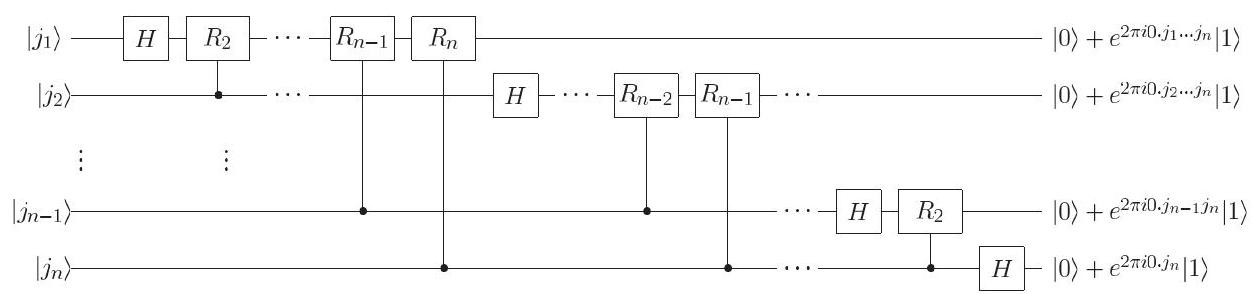
\includegraphics[width=1\linewidth]{Images/2024_05_17_6977ce60de6fd27aef98g-253}
\caption{Figure 5.1. Efficient circuit for the quantum Fourier transform. This circuit is easily derived from the product representation (5.4) for the quantum Fourier transform. Not shown are swap gates at the end of the circuit which reverse the order of the qubits, or normalization factors of $1 / \sqrt{2}$ in the output.}
\end{figure}

The product representation (5.4) makes it easy to derive an efficient circuit for the quantum Fourier transform. Such a circuit is shown in Figure 5.1. 

In Figure 5.1, the gate $R_{k}$ denotes the unitary transformation
\begin{equation}
    R_{k} \equiv\left[\begin{array}{cc}
1 & 0  \tag{5.11}\\
0 & e^{2 \pi i / 2^{k}}
\end{array}\right], \quad \forall k = 1,2,\dots,n.
\end{equation}
Note that $R_{k} |0\rangle = |0\rangle$ for all $k.$ When $k=1,$ $R_{1} |1\rangle = e^{2 \pi i\cdot 2^{-1}}|1\rangle = e^{2 \pi i\cdot (0.1)_2}|1\rangle$. When $k=2,$ $R_{2} |1\rangle = e^{2 \pi i\cdot 2^{-2}}|1\rangle = e^{2 \pi i\cdot (0.01)_2}|1\rangle.$ Similarly, for $k=1,2,\dots,n,$ one has
\begin{equation}
    R_{k} |1\rangle = e^{2 \pi i\cdot (0.0 \dots 1)_2}|1\rangle
\end{equation}
where the $(0.0 \dots \underbrace{1}_{k-th})_2=2^{-k}.$

To see that the pictured circuit computes the quantum Fourier transform, consider what happens when the state $\left|j_{1} \ldots j_{n}\right\rangle$ is input. 

Applying the Hadamard gate to the first bit produces the state
\begin{equation}
    |\psi_1\rangle:=\frac{1}{2^{1 / 2}}\left(|0\rangle+e^{2 \pi i 0 \cdot j_{1}}|1\rangle\right)\left|j_{2} \ldots j_{n}\right\rangle. \tag{5.12}
\end{equation}
In above, note that $0.j_1=0$ if $j_1=0$ and $0.j_1=\frac{1}{2}$ if $j_1=1.$ Thus, $e^{2 \pi i 0 . j_{1}}=1$  when $j_{1}=0$, and $e^{2 \pi i 0 . j_{1}}=-1$ when $j_{1}=1$.

Recall that applying the \textit{controlled-$R_{2}$ gate} to $|x_1 x_2 \rangle$ yields $(R_{2}^{x_2}|x_1\rangle) |x_2 \rangle$ when the controlled qubit is $x_2$ and target qubit is $x_1$, with $x_1,x_2=0,1.$ Thus, applying the controlled-$R_{2}$ gate to $|\psi_1\rangle$ produces the state
\begin{align}
&\frac{1}{2^{1 / 2}} \left( R_{2}^{j_2} \left(|0\rangle+e^{2 \pi i 0 \cdot j_{1}}|1\rangle\right) \right) \left|j_{2} \ldots j_{n}\right\rangle \\
=&\frac{1}{2^{1 / 2}}\left(R_{2}^{j_2} |0\rangle+e^{2 \pi i 0 \cdot j_{1} j_{2}}\cdot R_{2}^{j_2} |1\rangle\right)\left|j_{2} \ldots j_{n}\right\rangle \\
=&\frac{1}{2^{1 / 2}}\left(|0\rangle+e^{2 \pi i 0 \cdot j_{1} j_{2}}|1\rangle\right)\left|j_{2} \ldots j_{n}\right\rangle.     \tag{5.13}
\end{align}
It is easy to check the above equality holds for both $j_2=0$ and $j_2=1.$ 

We continue applying the \textit{controlled-$R_{3}, R_{4}$ through $R_{n}$ gates}, each of which adds an extra bit to the phase of the co-efficient of the first $|1\rangle$. At the end of this procedure we have the state
\begin{equation}
    \frac{1}{2^{1 / 2}}\left(|0\rangle+e^{2 \pi i 0 \cdot j_{1} j_{2} \ldots j_{n}}|1\rangle\right)\left|j_{2} \ldots j_{n}\right\rangle. \tag{5.14}
\end{equation}
Next, we perform a similar procedure on the second qubit. The Hadamard gate puts us in the state
\begin{equation}
    \frac{1}{2^{2 / 2}}\left(|0\rangle+e^{2 \pi i 0 \cdot j_{1} j_{2} \ldots j_{n}}|1\rangle\right)\left(|0\rangle+e^{2 \pi i 0 \cdot j_{2}}|1\rangle\right)\left|j_{3} \ldots j_{n}\right\rangle \tag{5.15}
\end{equation}
and the \textit{controlled-$R_{2}$ through $R_{n-1}$ gates} yield the state
\begin{equation}
    \frac{1}{2^{2 / 2}}\left(|0\rangle+e^{2 \pi i 0 \cdot j_{1} j_{2} \ldots j_{n}}|1\rangle\right)\left(|0\rangle+e^{2 \pi i 0 \cdot j_{2} \ldots j_{n}}|1\rangle\right)\left|j_{3} \ldots j_{n}\right\rangle. \tag{5.16}
\end{equation}
We continue in this fashion for each qubit, giving a final state
\begin{equation}
    \frac{1}{2^{n / 2}}\left(|0\rangle+e^{2 \pi i 0 \cdot j_{1} j_{2} \ldots j_{n}}|1\rangle\right)\left(|0\rangle+e^{2 \pi i 0 \cdot j_{2} \ldots j_{n}}|1\rangle\right) \ldots\left(|0\rangle+e^{2 \pi i 0 \cdot j_{n}}|1\rangle\right) \tag{5.17}
\end{equation}
Swap operations (see Section 1.3.4 for a description of the circuit), omitted from Figure 5.1 for clarity, are then used to reverse the order of the qubits. After the swap operations, the state of the qubits is
\begin{equation}
    \frac{1}{2^{n / 2}}\left(|0\rangle+e^{2 \pi i 0 \cdot j_{n}}|1\rangle\right)\left(|0\rangle+e^{2 \pi i 0 \cdot j_{n-1} j_{n}}|1\rangle\right) \ldots\left(|0\rangle+e^{2 \pi i 0 \cdot j_{1} j_{2} \cdots j_{n}}|1\rangle\right) \tag{5.18}
\end{equation}
Comparing with Equation (5.4) we see that this is the desired output from the quantum Fourier transform. 

This construction also proves that the quantum Fourier transform is unitary, since each gate in the circuit is unitary. An explicit example showing a circuit for the quantum Fourier transform on three qubits is given in Box 5.1.

\textbf{Box 5.1: Three qubit quantum Fourier transform}

For concreteness it may help to look at the explicit circuit for the three qubit quantum Fourier transform: 
\begin{figure}     
\centering
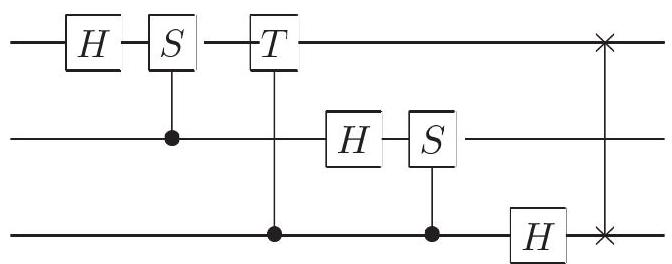
\includegraphics[width=0.75\linewidth]{Images/2024_05_17_6977ce60de6fd27aef98g-254}
\end{figure}
Recall that $S$ and $T$ are the phase and $\pi / 8$ gates. If the gate $R_{k}$ denotes the unitary transformation
\begin{equation}
    R_{k} \equiv\left[\begin{array}{cc}
1 & 0  \tag{5.11}\\
0 & e^{2 \pi i / 2^{k}}
\end{array}\right].
\end{equation}
Then, we have $R_2=S$ and $R_3=T.$

As a matrix the quantum Fourier transform in this instance may be written out explicitly, using $\omega=e^{2 \pi i / 8}=\sqrt{i}$, as
\begin{equation}
    \frac{1}{\sqrt{8}}\left[\begin{array}{cccccccc}
1 & 1 & 1 & 1 & 1 & 1 & 1 & 1  \tag{5.19}\\
1 & \omega & \omega^{2} & \omega^{3} & \omega^{4} & \omega^{5} & \omega^{6} & \omega^{7} \\
1 & \omega^{2} & \omega^{4} & \omega^{6} & 1 & \omega^{2} & \omega^{4} & \omega^{6} \\
1 & \omega^{3} & \omega^{6} & \omega^{1} & \omega^{4} & \omega^{7} & \omega^{2} & \omega^{5} \\
1 & \omega^{4} & 1 & \omega^{4} & 1 & \omega^{4} & 1 & \omega^{4} \\
1 & \omega^{5} & \omega^{2} & \omega^{7} & \omega^{4} & \omega^{1} & \omega^{6} & \omega^{3} \\
1 & \omega^{6} & \omega^{4} & \omega^{2} & 1 & \omega^{6} & \omega^{4} & \omega^{2} \\
1 & \omega^{7} & \omega^{6} & \omega^{5} & \omega^{4} & \omega^{3} & \omega^{2} & \omega^{1}
\end{array}\right] .
\end{equation}
You can find many materials about "matrix form of discrete Fourier transformation" on the internet.

\subsection{Discussion}

How many gates does this circuit use? 
\begin{itemize}
    \item We start by doing a Hadamard gate and $n-1$ conditional rotations on the first qubit - a total of $n$ gates.
    \item This is followed by a Hadamard gate and $n-2$ conditional rotations on the second qubit, for a total of $n-1$ gates.
    \item Continuing in this way, we see that $n+(n-1)+\cdots+1=n(n+1) / 2$ gates are required, plus the gates involved in the swaps.
    \item At most $n / 2$ swaps are required, and each swap can be accomplished using three controlled-NOT gates. 
\end{itemize}
Therefore, this circuit provides a $\Theta(n^{2})$ algorithm for performing the quantum Fourier transform.

In contrast, the best classical algorithms for computing the discrete Fourier transform on $2^{n}$ elements are algorithms such as the \textbf{Fast Fourier Transform (FFT)}, which compute the discrete Fourier transform using $\Theta\left(n 2^{n}\right)$ gates. That is, it requires exponentially more operations to compute the Fourier transform on a classical computer than it does to implement the quantum Fourier transform on a quantum computer.

Can we use the quantum Fourier transform to speed up the computation of these Fourier transforms? Unfortunately, the answer is that there is no known way to do this. 

\begin{enumerate}
    \item The problem is that the amplitudes in a quantum computer cannot be directly accessed by measurement. Thus, there is no way of determining the Fourier transformed amplitudes of the original state.
    \item Worse still, there is in general no way to efficiently prepare the original state to be Fourier transformed.
\end{enumerate}

In this and the next chapter we develop several algorithms based upon a more subtle application of the quantum Fourier transform.

\begin{exercise}
Exercise 5.3: (\textbf{Classical fast Fourier transform}) Suppose we wish to perform a Fourier transform of a vector containing $2^{n}$ complex numbers on a classical computer. Verify that the straightforward method for performing the Fourier transform, based upon direct evaluation of Equation (5.1) requires $\Theta\left(2^{2 n}\right)$ elementary arithmetic operations. Find a method for reducing this to $\Theta\left(n 2^{n}\right)$ operations, based upon Equation (5.4).
\end{exercise}

\begin{exercise}
\textbf{Exercise 5.4: Give a decomposition of the controlled-$R_{k}$ gate into single qubit and CNOT gates.}
\end{exercise}

\begin{exercise}
\textbf{Exercise 5.5: Give a quantum circuit to perform the inverse quantum Fourier transform.}
\end{exercise}

\begin{exercise}
\textbf{Exercise 5.6: (Approximate quantum Fourier transform)} The quantum circuit construction of the quantum Fourier transform apparently requires gates of exponential precision in the number of qubits used. However, such precision is never required in any quantum circuit of polynomial size. For example, let $U$ be the ideal quantum Fourier transform on $n$ qubits, and $V$ be the transform which results if the controlled-$R_{k}$ gates are performed to a precision $\Delta=1 / p(n)$ for some polynomial $p(n)$. Show that the error $E(U, V) \equiv \max _{|\psi\rangle} \|(U-V)|\psi\rangle \|$ scales as $\Theta\left(n^{2} / p(n)\right)$, and thus polynomial precision in each gate is sufficient to guarantee polynomial accuracy in the output state.
\end{exercise}


    % 2024-05-20 经LAI整理,已经初步完成

    \section{Phase Estimation}
    
The Fourier transform is the key to a general procedure known as phase estimation, which in turn is the key for many quantum algorithms. Suppose a unitary operator $U$ has an eigenvector $|u\rangle$ with eigenvalue $e^{2 \pi i \varphi}$, where the value of $\varphi$ is unknown. The goal of the phase estimation algorithm is to estimate $\varphi$. To perform the estimation we assume that we have available black boxes (sometimes known as oracles) capable of preparing the state $|u\rangle$ and performing the controlled- $-U^{2^{j}}$ operation, for suitable non-negative integers $j$. The use of black boxes indicates that the phase estimation procedure is not a complete quantum algorithm in its own right. Rather, you should think of phase estimation as a kind of 'subroutine' or 'module' that, when combined with other subroutines, can be used to perform interesting computational tasks. In specific applications of the phase estimation procedure we shall do exactly this, describing how these black box operations are to be performed, and combining them with the phase estimation procedure to do genuinely useful tasks. For the moment, though, we will continue to imagine them as black boxes.

The quantum phase estimation procedure uses two registers. The first register contains $t$ qubits initially in the state $|0\rangle$. How we choose $t$ depends on two things: the number of digits of accuracy we wish to have in our estimate for $\varphi$, and with what probability we wish the phase estimation procedure to be successful. The dependence of $t$ on these quantities emerges naturally from the following analysis.

The second register begins in the state $|u\rangle$, and contains as many qubits as is necessary to store $|u\rangle$. Phase estimation is performed in two stages. First, we apply the circuit shown in Figure 5.2. The circuit begins by applying a Hadamard transform to the first register, followed by application of controlled- $U$ operations on the second register, with $U$ raised\\
to successive powers of two. The final state of the first register is easily seen to be:

\begin{align}
\frac{1}{2^{t / 2}}\left(|0\rangle+e^{2 \pi i 2^{t-1} \varphi}|1\rangle\right)\left(|0\rangle+e^{2 \pi i 2^{t-2} \varphi}|1\rangle\right) & \ldots\left(|0\rangle+e^{2 \pi i 2^{0} \varphi}|1\rangle\right) \\
& =\frac{1}{2^{t / 2}} \sum_{k=0}^{2^{t}-1} e^{2 \pi i \varphi k}|k\rangle \tag{5.20}
\end{align} 

We omit the second register from this description, since it stays in the state $|u\rangle$ throughout the computation.

\begin{figure}
\centering
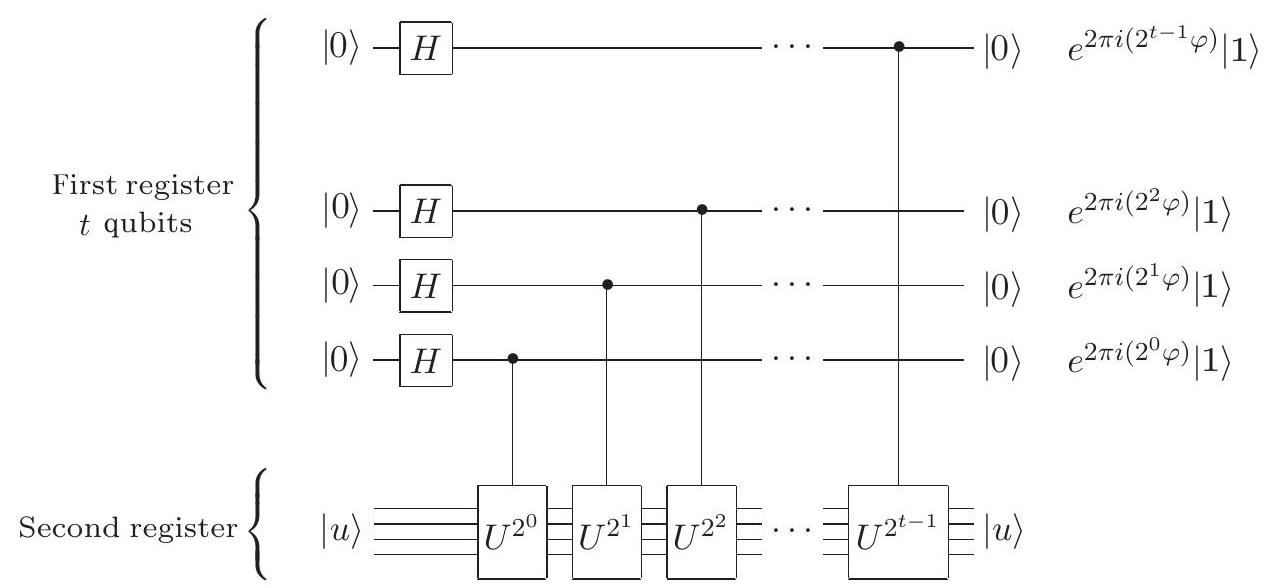
\includegraphics[width=0.75\linewidth]{Images/2024_05_17_6977ce60de6fd27aef98g-256}
\end{figure}

Figure 5.2. The first stage of the phase estimation procedure. Normalization factors of $1 / \sqrt{2}$ have been omitted, on the right.

Exercise 5.7: Additional insight into the circuit in Figure 5.2 may be obtained by showing, as you should now do, that the effect of the sequence of controlled- $U$ operations like that in Figure 5.2 is to take the state $|j\rangle|u\rangle$ to $|j\rangle U^{j}|u\rangle$. (Note that this does not depend on $|u\rangle$ being an eigenstate of $U$.)

The second stage of phase estimation is to apply the inverse quantum Fourier transform on the first register. This is obtained by reversing the circuit for the quantum Fourier transform in the previous section (Exercise 5.5), and can be done in $\Theta\left(t^{2}\right)$ steps. The third and final stage of phase estimation is to read out the state of the first register by doing a measurement in the computational basis. We will show that this provides a pretty good estimate of $\varphi$. An overall schematic of the algorithm is shown in Figure 5.3.

To sharpen our intuition as to why phase estimation works, suppose $\varphi$ may be expressed exactly in $t$ bits, as $\varphi=0 . \varphi_{1} \ldots \varphi_{t}$. Then the state (5.20) resulting from the first stage of phase estimation may be rewritten

\begin{equation}
    \frac{1}{2^{t / 2}}\left(|0\rangle+e^{2 \pi i 0 . \varphi_{t}}|1\rangle\right)\left(|0\rangle+e^{2 \pi i 0 . \varphi_{t-1} \varphi_{t}}|1\rangle\right) \ldots\left(|0\rangle+e^{2 \pi i 0 . \varphi_{1} \varphi_{2} \cdots \varphi_{t}}|1\rangle\right) \tag{5.21}
\end{equation}

The second stage of phase estimation is to apply the inverse quantum Fourier transform. But comparing the previous equation with the product form for the Fourier transform, Equation (5.4), we see that the output state from the second stage is the product state $\left|\varphi_{1} \ldots \varphi_{t}\right\rangle$. A measurement in the computational basis therefore gives us $\varphi$ exactly!

\begin{figure}
\centering
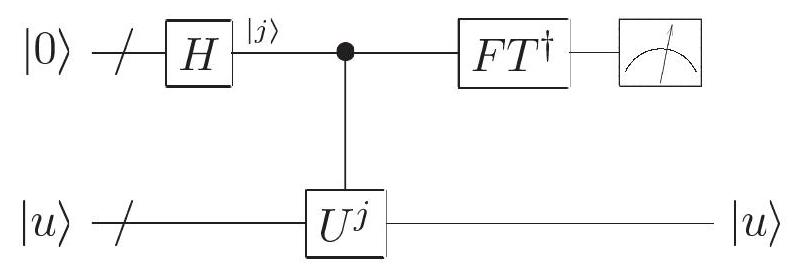
\includegraphics[width=0.75\linewidth]{Images/2024_05_17_6977ce60de6fd27aef98g-257}
\end{figure}

Figure 5.3. Schematic of the overall phase estimation procedure. The top $t$ qubits (the '/' denotes a bundle of wires, as usual) are the first register, and the bottom qubits are the second register, numbering as many as required to perform $U \cdot|u\rangle$ is an eigenstate of $U$ with eigenvalue $e^{2 \pi i \varphi}$. The output of the measurement is an approximation to $\varphi$ accurate to $t-\left\lceil\log \left(2+\frac{1}{2 \epsilon}\right)\right\rceil$ bits, with probability of success at least $1-\epsilon$.

Summarizing, the phase estimation algorithm allows one to estimate the phase $\varphi$ of an eigenvalue of a unitary operator $U$, given the corresponding eigenvector $|u\rangle$. An essential feature at the heart of this procedure is the ability of the inverse Fourier transform to perform the transformation

\begin{equation}
    \frac{1}{2^{t / 2}} \sum_{j=0}^{2^{t}-1} e^{2 \pi i \varphi j}|j\rangle|u\rangle \rightarrow|\tilde{\varphi}\rangle|u\rangle \tag{5.22}
\end{equation}

where $|\tilde{\varphi}\rangle$ denotes a state which is a good estimator for $\varphi$ when measured.

\subsection{Performance and Requirements}

The above analysis applies to the ideal case, where $\varphi$ can be written exactly with a $t$ bit binary expansion. What happens when this is not the case? It turns out that the procedure we have described will produce a pretty good approximation to $\varphi$ with high probability, as foreshadowed by the notation used in (5.22). Showing this requires some careful manipulations.

Let $b$ be the integer in the range 0 to $2^{t}-1$ such that $b / 2^{t}=0 . b_{1} \ldots b_{t}$ is the best $t$ bit approximation to $\varphi$ which is less than $\varphi$. That is, the difference $\delta \equiv \varphi-b / 2^{t}$ between $\varphi$ and $b / 2^{t}$ satisfies $0 \leq \delta \leq 2^{-t}$. We aim to show that the observation at the end of the phase estimation procedure produces a result which is close to $b$, and thus enables us to estimate $\varphi$ accurately, with high probability. Applying the inverse quantum Fourier transform to the state (5.20) produces the state

\begin{equation}
    \frac{1}{2^{t}} \sum_{k, l=0}^{2^{t}-1} e^{\frac{-2 \pi i k l}{2^{t}}} e^{2 \pi i \varphi k}|l\rangle \tag{5.23}
\end{equation}

Let $\alpha_{l}$ be the amplitude of $\left|(b+l)\left(\bmod 2^{t}\right)\right\rangle$,

\begin{equation}
    \alpha_{l} \equiv \frac{1}{2^{t}} \sum_{k=0}^{2^{t}-1}\left(e^{2 \pi i\left(\varphi-(b+l) / 2^{t}\right)}\right)^{k} \tag{5.24}
\end{equation}

This is the sum of a geometric series, so

\begin{equation}
    \alpha_{l}=\frac{1}{2^{t}}\left(\frac{1-e^{2 \pi i\left(2^{t} \varphi-(b+l)\right)}}{1-e^{2 \pi i\left(\varphi-(b+l) / 2^{t}\right)}}\right) \tag{5.25}
\end{equation}

\begin{equation}
    =\frac{1}{2^{t}}\left(\frac{1-e^{2 \pi i\left(2^{t} \delta-l\right)}}{1-e^{2 \pi i\left(\delta-l / 2^{t}\right)}}\right) \tag{5.26}
\end{equation}

Suppose the outcome of the final measurement is $m$. We aim to bound the probability of obtaining a value of $m$ such that $|m-b|>e$, where $e$ is a positive integer characterizing our desired tolerance to error. The probability of observing such an $m$ is given by

\begin{equation}
    p(|m-b|>e)=\sum_{-2^{t-1}<l \leq-(e+1)}\left|\alpha_{l}\right|^{2}+\sum_{e+1 \leq l \leq 2^{t-1}}\left|\alpha_{l}\right|^{2} \tag{5.27}
\end{equation}

But for any real $\theta,|1-\exp (i \theta)| \leq 2$, so

\begin{equation}
    \left|\alpha_{l}\right| \leq \frac{2}{2^{t} \mid 1-e^{2 \pi i\left(\delta-l / 2^{t}\right) \mid}} \tag{5.28}
\end{equation}

By elementary geometry or calculus $|1-\exp (i \theta)| \geq 2|\theta| / \pi$ whenever $-\pi \leq \theta \leq \pi$. But when $-2^{t-1}<l \leq 2^{t-1}$ we have $-\pi \leq 2 \pi\left(\delta-l / 2^{t}\right) \leq \pi$. Thus

\begin{equation}
    \left|\alpha_{l}\right| \leq \frac{1}{2^{t+1}\left(\delta-l / 2^{t}\right)} \tag{5.29}
\end{equation}

Combining (5.27) and (5.29) gives

\begin{equation}
    p(|m-b|>e) \leq \frac{1}{4}\left[\sum_{l=-2^{t-1}+1}^{-(e+1)} \frac{1}{\left(l-2^{t} \delta\right)^{2}}+\sum_{l=e+1}^{2^{t-1}} \frac{1}{\left(l-2^{t} \delta\right)^{2}}\right] \tag{5.30}
\end{equation}

Recalling that $0 \leq 2^{t} \delta \leq 1$, we obtain

\begin{align}
p(|m-b|>e) & \leq \frac{1}{4}\left[\sum_{l=-2^{t-1+1}}^{-(e+1)} \frac{1}{l^{2}}+\sum_{l=e+1}^{2^{t-1}} \frac{1}{(l-1)^{2}}\right]  \tag{5.31}\\
& \leq \frac{1}{2} \sum_{l=e}^{2^{t-1}-1} \frac{1}{l^{2}}  \tag{5.32}\\
& \leq \frac{1}{2} \int_{e-1}^{2^{t-1}-1} d l \frac{1}{l^{2}}  \tag{5.33}\\
& =\frac{1}{2(e-1)} \tag{5.34}
\end{align} 

Suppose we wish to approximate $\varphi$ to an accuracy $2^{-n}$, that is, we choose $e=2^{t-n}-1$. By making use of $t=n+p$ qubits in the phase estimation algorithm we see from (5.34) that the probability of obtaining an approximation correct to this accuracy is at least $1-1 / 2\left(2^{p}-2\right)$. Thus to successfully obtain $\varphi$ accurate to $n$ bits with probability of success at least $1-\epsilon$ we choose

\begin{equation}
    t=n+\left\lceil\log \left(2+\frac{1}{2 \epsilon}\right)\right\rceil \tag{5.35}
\end{equation}

In order to make use of the phase estimation algorithm, we need to be able to prepare an eigenstate $|u\rangle$ of $U$. What if we do not know how to prepare such an eigenstate? Suppose that we prepare some other state $|\psi\rangle$ in place of $|u\rangle$. Expanding this state in terms of eigenstates $|u\rangle$ of $U$ gives $|\psi\rangle=\sum_{u} c_{u}|u\rangle$. Suppose the eigenstate $|u\rangle$ has eigenvalue $e^{2 \pi i \varphi_{u}}$. Intuitively, the result of running the phase estimation algorithm will be to give\\
as output a state close to $\sum_{u} c_{u}\left|\widetilde{\varphi_{u}}\right\rangle|u\rangle$, where $\widetilde{\varphi_{u}}$ is a pretty good approximation to the phase $\varphi_{u}$. Therefore, we expect that reading out the first register will give us a good approximation to $\varphi_{u}$, where $u$ is chosen at random with probability $\left|c_{u}\right|^{2}$. Making this argument rigorous is left for Exercise 5.8. This procedure allows us to avoid preparing a (possibly unknown) eigenstate, at the cost of introducing some additional randomness into the algorithm.

Exercise 5.8: Suppose the phase estimation algorithm takes the state $|0\rangle|u\rangle$ to the state $\left|\widetilde{\varphi_{u}}\right\rangle|u\rangle$, so that given the input $|0\rangle\left(\sum_{u} c_{u}|u\rangle\right)$, the algorithm outputs $\sum_{u} c_{u}\left|\widetilde{\varphi_{u}}\right\rangle|u\rangle$. Show that if $t$ is chosen according to (5.35), then the probability for measuring $\varphi_{u}$ accurate to $n$ bits at the conclusion of the phase estimation algorithm is at least $\left|c_{u}\right|^{2}(1-\epsilon)$.

Why is phase estimation interesting? For its own sake, phase estimation solves a problem which is both non-trivial and interesting from a physical point of view: how to estimate the eigenvalue associated to a given eigenvector of a unitary operator. Its real use, though, comes from the observation that other interesting problems can be reduced to phase estimation, as will be shown in subsequent sections. The phase estimation algorithm is summarized below.

\textbf{Algorithm: Quantum phase estimation}

Inputs: (1) A black box wich performs a controlled- $U^{j}$ operation, for integer $j$, (2) an eigenstate $|u\rangle$ of $U$ with eigenvalue $e^{2 \pi i \varphi_{u}}$, and (3) $t=n+\left\lceil\log \left(2+\frac{1}{2 \epsilon}\right)\right\rceil$ qubits initialized to $|0\rangle$.

Outputs: An $n$-bit approximation $\widetilde{\varphi_{u}}$ to $\varphi_{u}$.

Runtime: $O\left(t^{2}\right)$ operations and one call to controlled- $U^{j}$ black box. Succeeds with probability at least $1-\epsilon$.

\textbf{Procedure:}
\begin{enumerate}
    \item $\quad|0\rangle|u\rangle$
\end{enumerate}

initial state\\
2. $\quad \rightarrow \frac{1}{\sqrt{2^{t}}} \sum_{j=0}^{2^{t}-1}|j\rangle|u\rangle$

create superposition\\
3. $\left.\quad \rightarrow \frac{1}{\sqrt{2^{t}}} \sum_{j=0}^{2^{t}-1}|j\rangle U^{j} \right\rvert\, u$

apply black box

$=\frac{1}{\sqrt{2^{t}}} \sum_{j=0}^{2^{t}-1} e^{2 \pi i j \varphi_{u}}|j\rangle|u\rangle$

result of black box\\
4. $\quad \rightarrow\left|\widetilde{\varphi_{u}}\right\rangle|u\rangle$

apply inverse Fourier transform\\
5. $\quad \rightarrow \widetilde{\varphi_{u}}$

measure first register

Exercise 5.9: Let $U$ be a unitary transform with eigenvalues $\pm 1$, which acts on a state $|\psi\rangle$. Using the phase estimation procedure, construct a quantum circuit to collapse $|\psi\rangle$ into one or the other of the two eigenspaces of $U$, giving also a\\
classical indicator as to which space the final state is in. Compare your result with Exercise 4.34.
    % 2024-05-20 经LAI整理,已经初步完成

    \section{Applications: Order-finding and Factoring}
    % \input{Applications: order-finding and factoring}
    % 有待整理

    \section{General Applications of the Quantum Fourier Transform}
    
\section{5.4 General Applications of the Quantum Fourier Transform}

The main applications of the quantum Fourier transform we have described so far in this chapter are phase estimation and order-finding. What other problems can be solved with these techniques? In this section, we define a very general problem known as the hidden subgroup problem, and describe an efficient quantum algorithm for solving it. This problem, which encompasses all known 'exponentially fast' applications of the quantum Fourier transform, can be thought of as a generalization of the task of finding the unknown period of a periodic function, in a context where the structure of the domain and range

\textbf{Box5.4: Factoring 15 quantum-mechanically}
The use of order-finding, phase estimation, and continued fraction expansions in the quantum factoring algorithm is illustrated by applying it to factor $N=15$. First, we choose a random number which has no common factors with $N$; suppose we choose $x=7$. Next, we compute the order $r$ of $x$ with respect to $N$, using the quantum order-finding algorithm: begin with the state $|0\rangle|0\rangle$ and create the state

\begin{equation}
    \frac{1}{\sqrt{2^{t}}} \sum_{k=0}^{2^{t}-1}|k\rangle|0\rangle=\frac{1}{\sqrt{2^{t}}}\left[|0\rangle+|1\rangle+|2\rangle+\cdots+\left|2^{t}-1\right\rangle\right]|0\rangle \tag{5.61}
\end{equation}

by applying $t=11$ Hadamard transforms to the first register. Choosing this value of $t$ ensures an error probability $\epsilon$ of at most $1 / 4$. Next, compute $f(k)=x^{k} \bmod N$, leaving the result in the second register,
\begin{align}
& \frac{1}{\sqrt{2^{t}}} \sum_{k=0}^{2^{t}-1}|k\rangle\left|x^{k} \bmod N\right\rangle  \tag{5.62}\\
& =\frac{1}{\sqrt{2^{t}}}[|0\rangle|1\rangle+|1\rangle|7\rangle+|2\rangle|4\rangle+|3\rangle|13\rangle+|4\rangle|1\rangle+|5\rangle|7\rangle+|6\rangle|4\rangle+\cdots]
\end{align}

We now apply the inverse Fourier transform $F T^{\dagger}$ to the first register and measure it. One way of analyzing the distribution of outcomes obtained is to calculate the reduced density matrix for the first register, and apply $F T^{\dagger}$ to it, and calculate the measurement statistics. However, since no further operation is applied to the second register, we can instead apply the principle of implicit measurement (Section 4.4) and assume that the second register is measured, obtaining a random result from 1, 7,4 , or 13 . Suppose we get 4 (any of the results works); this means the state input to $F T^{\dagger}$ would have been $\sqrt{\frac{4}{2^{t}}}[|2\rangle+|6\rangle+|10\rangle+|14\rangle+\cdots]$. After applying $F T^{\dagger}$ we obtain some state $\sum_{\ell} \alpha_{\ell}|\ell\rangle$, with the probability distribution

\begin{figure}
\centering
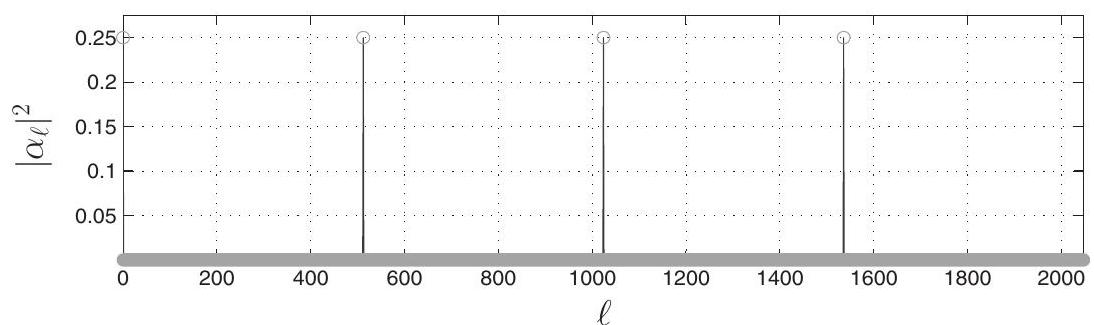
\includegraphics[width=0.75\linewidth]{Images/2024_05_17_6977ce60de6fd27aef98g-269}
\end{figure}

shown for $2^{t}=2048$. The final measurement therefore gives either $0,512,1024$, or 1536 , each with probability almost exactly $1 / 4$. Suppose we obtain $\ell=1536$ from the measurement; computing the continued fraction expansion thus gives $1536 / 2048=1 /(1+(1 / 3))$, so that $3 / 4$ occurs as a convergent in the expansion, giving $r=4$ as the order of $x=7$. By chance, $r$ is even, and moreover, $x^{r / 2} \bmod N=7^{2} \bmod 15=4 \neq-1 \bmod 15$, so the algorithm works: computing the greatest common divisor $\operatorname{gcd}\left(x^{2}-1,15\right)=3$ and $\operatorname{gcd}\left(x^{2}+1,15\right)=5$ tells us that $15=3 \times 5$.\\
of the function may be very intricate. In order to present this problem in the most approachable manner, we begin with two more specific applications: period-finding (of a one-dimensional function), and discrete logarithms. We then return to the general hidden subgroup problem. Note that the presentation in this section is rather more schematic and conceptual than earlier sections in this chapter; of necessity, this means that the reader interested in understanding all the details will have to work much harder!

\subsection{5.4.1 Period-finding}
Consider the following problem. Suppose $f$ is a periodic function producing a single bit as output and such that $f(x+r)=f(x)$, for some unknown $0<r<2^{L}$, where $x, r \in\{0,1,2, \ldots\}$. Given a quantum black box $U$ which performs the unitary transform $U|x\rangle|y\rangle \rightarrow|x\rangle|y \oplus f(x)\rangle$ (where $\oplus$ denotes addition modulo 2) how many black box queries and other operations are required to determine $r$ ? Note that in practice $U$ operates on a finite domain, whose size is determined by the desired accuracy for $r$. Here is a quantum algorithm which solves this problem using one query, and $O\left(L^{2}\right)$ other operations:

\textbf{Algorithm: Period-finding}
Inputs: (1) A black box which performs the operation $U|x\rangle|y\rangle=|x\rangle|y \oplus f(x)\rangle$, (2) a state to store the function evaluation, initialized to $|0\rangle$, and (3) $t=O(L+\log (1 / \epsilon))$ qubits initialized to $|0\rangle$.

Outputs: The least integer $r>0$ such that $f(x+r)=f(x)$.

Runtime: One use of $U$, and $O\left(L^{2}\right)$ operations. Succeeds with probability $O(1)$.

\textbf{Procedure:}
\begin{enumerate}
    \item $\quad|0\rangle|0\rangle$
    \item $\rightarrow \frac{1}{\sqrt{2^{t}}} \sum_{x=0}^{2^{t}-1}|x\rangle|0\rangle$
    \item $\rightarrow \frac{1}{\sqrt{2^{t}}} \sum_{x=0}^{2^{t}-1}|x\rangle|f(x)\rangle$

\end{enumerate}

$\approx \frac{1}{\sqrt{r 2^{t}}} \sum_{\ell=0}^{r-1} \sum_{x=0}^{2^{t}-1} e^{2 \pi i \ell x / r}|x\rangle|\hat{f}(\ell)\rangle$

\begin{enumerate}
  \setcounter{enumi}{3}
    \item $\left.\quad \rightarrow \frac{1}{\sqrt{r}} \sum_{\ell=0}^{r-1}|\widetilde{\ell / r\rangle}| \hat{f}(\ell)\right\rangle$
    \item $\quad \rightarrow \widetilde{\ell / r}$
    \item $\rightarrow r$ initial state

\end{enumerate}

create superposition

apply $U$

apply inverse Fourier transform to first register

measure first register

apply continued fractions algorithm

The key to understanding this algorithm, which is based on phase estimation, and is nearly identical to the algorithm for quantum order-finding, is step 3 , in which we introduce the state

\begin{equation}
    |\hat{f}(\ell)\rangle \equiv \frac{1}{\sqrt{r}} \sum_{x=0}^{r-1} e^{-2 \pi i \ell x / r}|f(x)\rangle \tag{5.63}
\end{equation}

the Fourier transform of $|f(x)\rangle$. The identity used in step 3 is based on

\begin{equation}
    |f(x)\rangle=\frac{1}{\sqrt{r}} \sum_{\ell=0}^{r-1} e^{2 \pi i \ell x / r}|\hat{f}(\ell)\rangle \tag{5.64}
\end{equation}

which is easy to verify by noting that $\sum_{\ell=0}^{r-1} e^{2 \pi i \ell x / r}=r$ for $x$ an integer multiple of $r$, and zero otherwise. The approximate equality in step 3 is required because $2^{t}$ may not be an integer multiple of $r$ in general (it need not be: this is taken account of by the phase estimation bounds). By Equation (5.22), applying the inverse Fourier transform to the first register, in step 4 , gives an estimate of the phase $\ell / r$, where $\ell$ is chosen randomly. $r$ can be efficiently obtained in the final step using a continued fraction expansion.

\textbf{Box5.5: The shift-invariance property of the Fourier transform}
The Fourier transform, Equation (5.1), has an interesting and very useful property, known as shift invariance. Using notation which is useful in describing the general application of this property, let us describe the quantum Fourier transform as

\begin{equation}
    \sum_{h \in H} \alpha_{h}|h\rangle \rightarrow \sum_{g \in G} \tilde{\alpha}_{g}|g\rangle, \tag{5.65}
\end{equation}

where $\tilde{\alpha}_{g}=\sum_{h \in H} \alpha_{h} \exp (2 \pi i g h /|G|), H$ is some subset of $G$, and $G$ indexes the states in an orthonormal basis of the Hilbert space. For example, $G$ may be the set of numbers from 0 to $2^{n}-1$ for an $n$ qubit system. $|G|$ denotes the number of elements in $G$. Suppose we apply to the initial state an operator $U_{k}$ which performs the unitary transform

\begin{equation}
    U_{k}|g\rangle=|g+k\rangle, \tag{5.66}
\end{equation}

then apply the Fourier transform. The result,

\begin{equation}
    U_{k} \sum_{h \in H} \alpha_{h}|h\rangle=\sum_{h \in H} \alpha_{h}|h+k\rangle \rightarrow \sum_{g \in G} e^{2 \pi i g k /|G|} \tilde{\alpha}_{g}|g\rangle \tag{5.67}
\end{equation}

has the property that the magnitude of the amplitude for $|g\rangle$ does not change, no matter what $k$ is, that is: $\left|\exp (2 \pi i g k /|G|) \tilde{\alpha}_{g}\right|=\left|\tilde{\alpha}_{g}\right|$.

In the language of group theory, $G$ is a group, $H$ a subgroup of $G$, and we say that if a function $f$ on $G$ is constant on cosets of $H$, then the Fourier transform of $f$ is invariant over cosets of $H$.

Why does this work? One way to understand this is to realize that (5.63) is approximately the Fourier transform over $\left\{0,1, \ldots, 2^{L}-1\right\}$ of $|f(x)\rangle$ (see Exercise 5.20), and the Fourier transform has an interesting and very useful property, known as shift invariance, described in Box 5.5. Another is to realize that what the order-finding algorithm does is just to find the period of the function $f(k)=x^{k} \bmod N$, so the ability to find the period of a general periodic function is not unexpected. Yet another way is to realize that the implementation of the black box $U$ is naturally done using a certain unitary operator whose eigenvectors are precisely $|\hat{f}(\ell)\rangle$, as described in Exercise 5.21 below, so that the phase estimation procedure of Section 5.2 can be applied.

Exercise 5.20: Suppose $f(x+r)=f(x)$, and $0 \leq x<N$, for $N$ an integer multiple of $r$. Compute

\begin{equation}
    \hat{f}(\ell) \equiv \frac{1}{\sqrt{N}} \sum_{x=0}^{N-1} e^{-2 \pi i \ell x / N} f(x) \tag{5.68}
\end{equation}

and relate the result to (5.63). You will need to use the fact that

\begin{equation}
    \sum_{k \in\{0, r, 2 r, \ldots, N-r\}} e^{2 \pi i k \ell / N}= \begin{cases}\sqrt{N / r} & \text { if } \ell \text { is an integer multiple of } N / r  \tag{5.69}\\ 0 & \text { otherwise. }\end{cases}
\end{equation}

Exercise 5.21: (Period-finding and phase estimation) Suppose you are given a unitary operator $U_{y}$ which performs the transformation $U_{y}|f(x)\rangle=|f(x+y)\rangle$, for the periodic function described above.

(1) Show that the eigenvectors of $U_{y}$ are $|\hat{f}(\ell)\rangle$, and calculate their eigenvalues.

(2) Show that given $\left|f\left(x_{0}\right)\right\rangle$ for some $x_{0}, U_{y}$ can be used to realize a black box which is as useful as $U$ in solving the period-finding problem.

\subsection{5.4.2 Discrete Logarithms}
The period finding problem we just considered is a simple one, in that the domain and range of the periodic function were integers. What happens when the function is more complex? Consider the function $f\left(x_{1}, x_{2}\right)=a^{s x_{1}+x_{2}} \bmod N$, where all the variables are integers, and $r$ is the smallest positive integer for which $a^{r} \bmod N=1$. This function is periodic, since $f\left(x_{1}+\ell, x_{2}-\ell s\right)=f\left(x_{1}, x_{2}\right)$, but now the period is a 2-tuple, $(\ell,-\ell s)$, for integer $\ell$. This may seem to be a strange function, but it is very useful in cryptography, since determining $s$ allows one to solve what is known as the discrete logarithm problem: given $a$ and $b=a^{s}$, what is $s$ ? Here is a quantum algorithm which solves this problem using one query of a quantum black box $U$ which performs the unitary transform $U\left|x_{1}\right\rangle\left|x_{2}\right\rangle|y\rangle \rightarrow\left|x_{1}\right\rangle\left|x_{2}\right\rangle|y \oplus f(x)\rangle($ where $\oplus$ denotes bitwise addition modulo 2), and $O\left(\lceil\log r\rceil^{2}\right)$ other operations. We assume knowledge of the minimum $r>0$ such that $a^{r} \bmod N=1$, which can be obtained using the order-finding algorithm described previously.

\textbf{Algorithm: Discrete logarithm}
Inputs: (1) A black box which performs the operation

$U\left|x_{1}\right\rangle\left|x_{2}\right\rangle|y\rangle=\left|x_{1}\right\rangle\left|x_{2}\right\rangle\left|y \oplus f\left(x_{1}, x_{2}\right)\right\rangle$, for $f\left(x_{1}, x_{2}\right)=b^{x_{1}} a^{x_{2}},(2)$ a state to store the function evaluation, initialized to $|0\rangle$, and (3) two $t=O(\lceil\log r\rceil+\log (1 / \epsilon))$ qubit registers initialized to $|0\rangle$.

Outputs: The least positive integer $s$ such that $a^{s}=b$.

Runtime: One use of $U$, and $O\left(\lceil\log r\rceil^{2}\right)$ operations. Succeeds with probability $O(1)$.

\textbf{Procedure:}
\begin{enumerate}
    \item $\quad|0\rangle|0\rangle|0\rangle$
\end{enumerate}

initial state\\
2. $\quad \rightarrow \frac{1}{2^{t}} \sum_{x_{1}=0}^{2^{t}-1} \sum_{x_{2}=0}^{2^{t}-1}\left|x_{1}\right\rangle\left|x_{2}\right\rangle|0\rangle \quad$ create superposition\\
3. $\quad \rightarrow \frac{1}{2^{t}} \sum_{x_{1}=0}^{2^{t}-1} \sum_{x_{2}=0}^{2^{t}-1}\left|x_{1}\right\rangle\left|x_{2}\right\rangle\left|f\left(x_{1}, x_{2}\right)\right\rangle \quad$ apply $U$ $\approx \frac{1}{2^{t} \sqrt{r}} \sum_{\ell_{2}=0}^{r-1} \sum_{x_{1}=0}^{2^{t}-1} \sum_{x_{2}=0}^{2^{t}-1} e^{2 \pi i\left(s \ell_{2} x_{1}+\ell_{2} x_{2}\right) / r}\left|x_{1}\right\rangle\left|x_{2}\right\rangle\left|\hat{f}\left(s \ell_{2}, \ell_{2}\right)\right\rangle$ $=\frac{1}{2^{t} \sqrt{r}} \sum_{\ell_{2}=0}^{r-1}\left[\sum_{x_{1}=0}^{2^{t}-1} e^{2 \pi i\left(s \ell_{2} x_{1}\right) / r}\left|x_{1}\right\rangle\right]\left[\sum_{x_{2}=0}^{2^{t}-1} e^{2 \pi i\left(\ell_{2} x_{2}\right) / r}\left|x_{2}\right\rangle\right]\left|\hat{f}\left(s \ell_{2}, \ell_{2}\right)\right\rangle$\\
4. $\left.\quad \rightarrow \frac{1}{\sqrt{r}} \sum_{\ell_{2}=0}^{r-1}\left|\widetilde{\ell_{2} / r} r\right| \widetilde{\ell_{2} / r}\right\rangle\left|\hat{f}\left(s \ell_{2}, \ell_{2}\right)\right\rangle \quad$ apply inverse Fourier transform to first\\
5. $\rightarrow\left(\widetilde{s \ell_{2} / r}, \widetilde{\ell_{2} / r}\right) \quad$ measure first two registers\\
6. $\quad \rightarrow s$

apply generalized continued fractions algorithm

Again, the key to understanding this algorithm is step 3 , in which we introduce the state

\begin{equation}
    \left|\hat{f}\left(\ell_{1}, \ell_{2}\right)\right\rangle=\frac{1}{\sqrt{r}} \sum_{j=0}^{r-1} e^{-2 \pi i \ell_{2} j / r}|f(0, j)\rangle \tag{5.70}
\end{equation}

the Fourier transform of $\left|f\left(x_{1}, x_{2}\right)\right\rangle$ (see Exercise 5.22). In this equation, the values of $\ell_{1}$ and $\ell_{2}$ must satisfy

\begin{equation}
    \sum_{k=0}^{r-1} e^{2 \pi i k\left(\ell_{1} / s-\ell_{2}\right) / r}=r \tag{5.71}
\end{equation}

Otherwise, the amplitude of $\left|\hat{f}\left(\ell_{1}, \ell_{2}\right)\right\rangle$ is nearly zero. The generalized continued fraction expansion used in the final step to determine $s$ is analogous to the procedures used in Section 5.3.1, and is left as a simple exercise for you to construct.

Exercise 5.22: Show that

\begin{equation}
    \left|\hat{f}\left(\ell_{1}, \ell_{2}\right)\right\rangle=\sum_{x_{1}=0}^{r-1} \sum_{x_{2}=0}^{r-1} e^{-2 \pi i\left(\ell_{1} x_{1}+\ell_{2} x_{2}\right) / r}\left|f\left(x_{1}, x_{2}\right)\right\rangle=\frac{1}{\sqrt{r}} \sum_{j=0}^{r-1} e^{-2 \pi i \ell_{2} j / r}|f(0, j)\rangle \tag{5.72}
\end{equation}

and we are constrained to have $\ell_{1} / s-\ell_{2}$ be an integer multiple of $r$ for this expression to be non-zero.

Exercise 5.23: Compute

\begin{equation}
    \frac{1}{r} \sum_{\ell_{1}=0}^{r-1} \sum_{\ell_{2}=0}^{r-1} e^{-2 \pi i\left(\ell_{1} x_{1}+\ell_{2} x_{2}\right) / r}\left|\hat{f}\left(\ell_{1}, \ell_{2}\right)\right\rangle \tag{5.73}
\end{equation}

using (5.70), and show that the result is $f\left(x_{1}, x_{2}\right)$.

Exercise 5.24: Construct the generalized continued fractions algorithm needed in\\
step 6 of the discrete logarithm algorithm to determine $s$ from estimates of $s \ell_{2} / r$ and $\ell_{2} / r$.

Exercise 5.25: Construct a quantum circuit for the black box $U$ used in the quantum discrete logarithm algorithm, which takes $a$ and $b$ as parameters, and performs the unitary transform $\left|x_{1}\right\rangle\left|x_{2}\right\rangle|y\rangle \rightarrow\left|x_{1}\right\rangle\left|x_{2}\right\rangle\left|y \oplus b^{x_{1}} a^{x_{2}}\right\rangle$. How many elementary operations are required?

\subsection{5.4.3 The Hidden Subgroup Problem}
By now, a pattern should be coming clear: if we are given a periodic function, even when the structure of the periodicity is quite complicated, we can often use a quantum algorithm to determine the period efficiently. Importantly, however, not all periods of periodic functions can be determined. The general problem which defines a broad framework for these questions can be succinctly expressed in the language of group theory (see Appendix 2 for a quick review) as follows:

Let $f$ be a function from a finitely generated group $G$ to a finite set $X$ such that $f$ is constant on the cosets of a subgroup $K$, and distinct on each coset. Given a quantum black box for performing the unitary transform $U|g\rangle|h\rangle=|g\rangle|h \oplus f(g)\rangle$, for $g \in G, h \in X$, and $\oplus$ an appropriately chosen binary operation on $X$, find a generating set for $K$.

Order-finding, period-finding, discrete logarithms, and many other problems are instances of this hidden subgroup problem; some interesting ones are listed in Figure 5.5.

For $G$ a finite Abelian group, a quantum computer can solve the hidden subgroup problem using a number of operations polynomial in $\log |G|$, and one use of the black box function evaluation, using an algorithm very similar to the others in this section. (In fact, solution for a finitely generated Abelian group is also possible, along similar lines, but we'll stick to the finite case here.) We shall leave detailed specification of the algorithm to you as an exercise, which should be simple after we explain the basic idea. Many things remain essentially the same, because finite Abelian groups are isomorphic to products of additive groups over the integers in modular arithmetic. This means that the quantum Fourier transform of $f$ over $G$ is well defined (see Section A2.3), and can still be done efficiently. The first non-trivial step of the algorithm is to use a Fourier transform (generalizing the Hadamard operation) to create a superposition over group elements, which is then transformed by applying the quantum black box for $f$ in the next step, to give

\begin{equation}
    \frac{1}{\sqrt{|G|}} \sum_{g \in G}|g\rangle|f(g)\rangle \tag{5.74}
\end{equation}

As before, we would now like to rewrite $|f(g)\rangle$ in the Fourier basis. We start with

\begin{equation}
    |f(g)\rangle=\frac{1}{\sqrt{|G|}} \sum_{\ell=0}^{|G|-1} e^{2 \pi i \ell g /|G|}|\hat{f}(\ell)\rangle \tag{5.75}
\end{equation}

where we have chosen $\exp [-2 \pi i \ell g /|G|]$ as a representation (see Exercise A2.13) of $g \in G$ indexed by $\ell$ (the Fourier transform maps between group elements and representations: see Exercise A2.23). The key is to recognize that this expression can be simplified because

\begin{center}
\begin{tabular}{|c|c|c|c|c|}
\hline
Name & $G$ & $X$ & K & Function \\
\hline
Deutsch & $\{0,1\}, \oplus$ & $\{0,1\}$ & $\{0\}$ or $\{0,1\}$ & \begin{tabular}{l}
$K=\{0,1\}:\left\{\begin{array}{l}f(x)=0 \\ f(x)=1\end{array}\right.$ \\
$K=\{0\}:\left\{\begin{array}{l}f(x)=x \\ f(x)=1-x\end{array}\right.$ \\
\end{tabular} \\
\hline
Simon & $\{0,1\}^{n}, \oplus$ & \begin{tabular}{l}
any \\
finite \\
set \\
\end{tabular} & \begin{tabular}{c}
$\{0, s\}$ \\
$s \in\{0,1\}^{n}$ \\
\end{tabular} & $f(x \oplus s)=f(x)$ \\
\hline
\begin{tabular}{l}
Period- \\
finding \\
\end{tabular} & $\mathrm{Z},++$ & \begin{tabular}{l}
any \\
finite \\
set \\
\end{tabular} & \begin{tabular}{l}
$\{0, r, 2 r, \ldots\}$ \\
$\quad r \in G$ \\
\end{tabular} & $f(x+r)=f(x)$ \\
\hline
\begin{tabular}{l}
Order- \\
finding \\
\end{tabular} & $\mathrm{Z},+$ & \begin{tabular}{l}
$\left\{a^{j}\right\}$ \\
$j \in Z_{r}$ \\
$a^{r}=1$ \\
\end{tabular} & \begin{tabular}{c}
$\{0, r, 2 r, \ldots\}$ \\
$r \in G$ \\
\end{tabular} & \begin{tabular}{l}
$f(x)=a^{x}$ \\
$f(x+r)=f(x)$ \\
\end{tabular} \\
\hline
\begin{tabular}{l}
Discrete \\
logarithm \\
\end{tabular} & \begin{tabular}{c}
$\mathbf{Z}_{r} \times \mathbf{Z}_{r}$ \\
$+(\bmod r)$ \\
\end{tabular} & \begin{tabular}{l}
$\left\{a^{j}\right\}$ \\
$j \in Z_{r}$ \\
$a^{r}=1$ \\
\end{tabular} & \begin{tabular}{l}
$(\ell,-\ell s)$ \\
$\ell, s \in \mathbf{Z}_{r}$ \\
\end{tabular} & \begin{tabular}{l}
$f\left(x_{1}, x_{2}\right)=a^{k x_{1}+x_{2}}$ \\
$f\left(x_{1}+\ell, x_{2}-\ell s\right)=f\left(x_{1}, x_{2}\right)$ \\
\end{tabular} \\
\hline
\begin{tabular}{l}
Order of a \\
permutation \\
\end{tabular} & \begin{tabular}{l}
$\mathbf{Z}_{2^{m}} \times \mathbf{Z}_{2^{n}}$ \\
$+\left(\bmod 2^{m}\right)$ \\
\end{tabular} & $\mathbf{Z}_{2^{n}}$ & \begin{tabular}{l}
$\{0, r, 2 r, \ldots\}$ \\
$\quad r \in X$ \\
\end{tabular} & \begin{tabular}{l}
$f(x, y)=\pi^{x}(y)$ \\
$f(x+r, y)=f(x, y)$ \\
$\pi=$ permutation on $X$ \\
\end{tabular} \\
\hline
\begin{tabular}{l}
Hidden \\
linear \\
function \\
\end{tabular} & $\mathbf{Z} \times \mathbf{Z},+$ & $\mathbf{Z}_{N}$ & \begin{tabular}{l}
$(\ell,-\ell s)$ \\
$\ell, s \in X$ \\
\end{tabular} & \begin{tabular}{l}
$f\left(x_{1}, x_{2}\right)=$ \\
$\quad \pi\left(s x_{1}+x_{2} \bmod N\right)$ \\
$\pi=$ permutation on $X$ \\
\end{tabular} \\
\hline
\begin{tabular}{l}
Abelian \\
stabilizer \\
\end{tabular} & \begin{tabular}{l}
$(H, X)$ \\
$H=$ any \\
Abelian \\
group \\
\end{tabular} & \begin{tabular}{l}
any \\
finite \\
set \\
\end{tabular} & \begin{tabular}{l}
$\{s \in H \mid$ \\
$f(s, x)=x$ \\
$\forall x \in X\}$ \\
\end{tabular} & \begin{tabular}{l}
$f(g h, x)=f(g, f(h, x))$ \\
$f(g s, x)=f(g, x)$ \\
\end{tabular} \\
\hline
\end{tabular}
\end{center}

Figure 5.5. Hidden subgroup problems. The function $f$ maps from the group $G$ to the finite set $X$, and is promised to be constant on cosets of the hidden subgroup $K \subseteq G . \mathbf{Z}_{N}$ represents the set $\{0,1, \ldots, N-1\}$ in this table, and $\mathbf{Z}$ is the integers. The problem is to find $K$ (or a generating set for it), given a black box for $f$.

$f$ is constant and distinct on cosets of the subgroup $K$, so that

\begin{equation}
    |\hat{f}(\ell)\rangle=\frac{1}{\sqrt{|G|}} \sum_{g \in G} e^{-2 \pi i \ell g /|G|}|f(g)\rangle \tag{5.76}
\end{equation}

has nearly zero amplitude for all values of $\ell$ except those which satisfy

\begin{equation}
    \sum_{h \in K} e^{-2 \pi i \ell h /|G|}=|K| \tag{5.77}
\end{equation}

If we can determine $\ell$, then using the linear constraints given by this expression allows us to determine elements of $K$, and since $K$ is Abelian, this allows us to eventually determine a generating set for the whole hidden subgroup, solving the problem.

However, life is not so simple. An important reason why the period-finding and discrete logarithm algorithms work is because of the success of the continued fraction expansion in obtaining $\ell$ from $\ell /|G|$. In those problems, $\ell$ and $|G|$ are arranged to not have any common factors, with high probability. In the general case, however, this may not be true, since $|G|$ is free to be a composite number with many factors, and we have no useful prior information about $\ell$.

Fortunately, this problem can be solved: as mentioned above, any finite Abelian group $G$ is isomorphic to a product of cyclic groups of prime power order, that is, $G=\mathbf{Z}_{p_{1}} \times$ $\mathbf{Z}_{p_{2}} \times \cdots \times \mathbf{Z}_{p_{M}}$, where $p_{i}$ are primes, and $\mathbf{Z}_{p_{i}}$ is the group over integers $\left\{0,1, \ldots, p_{i}-1\right\}$ with addition modulo $p_{i}$ being the group operation. We can thus re-express the phase which appears in $(5.75)$ as

\begin{equation}
    e^{2 \pi i \ell g /|G|}=\prod_{i=1}^{M} e^{2 \pi i \ell_{i}^{\prime} g_{i} / p_{i}} \tag{5.78}
\end{equation}

for $g_{i} \in \mathbf{Z}_{p_{i}}$. The phase estimation procedure now gives us $\ell_{i}^{\prime}$, from which we determine $\ell$, and thus, sample $K$ as described above, to solve the hidden subgroup problem.

Exercise 5.26: $\quad$ Since $K$ is a subgroup of $G$, when we decompose $G$ into a product of cyclic groups of prime power order, this also decomposes $K$. Re-express (5.77) to show that determining $\ell_{i}^{\prime}$ allows one to sample from the corresponding cyclic subgroup $K_{p_{i}}$ of $K$.

Exercise 5.27: Of course, the decomposition of a general finite Abelian group $G$ into a product of cyclic groups of prime power order is usually a difficult problem (at least as hard as factoring integers, for example). Here, quantum algorithms come to the rescue again: explain how the algorithms in this chapter can be used to efficiently decompose $G$ as desired.

Exercise 5.28: Write out a detailed specification of the quantum algorithm to solve the hidden subgroup problem, complete with runtime and success probability estimates, for finite Abelian groups.

Exercise 5.29: Give quantum algorithms to solve the Deutsch and Simon problems listed in Figure 5.5, using the framework of the hidden subgroup problem.

\subsection{5.4.4 Other Quantum Algorithms?}
One of the most intriguing aspects of this framework for describing quantum algorithms in terms of the hidden subgroup problem is the suggestion that more difficult problems might be solvable by considering various groups $G$ and functions $f$. We have only described the solution of this problem for Abelian groups. What about non-Abelian groups? They are quite interesting (see Appendix 2 for a discussion of general Fourier transforms over non-Abelian groups): for example, the problem of graph isomorphism is to determine if two given graphs are the same under some permutation of the labels of the $n$ vertices (Section 3.2.3). These permutations can be described as transformations under the symmetric group $S_{n}$, and algorithms for performing fast Fourier transforms\\
over these groups exists. However, a quantum algorithm for efficiently solving the graph isomporphism problem remains unknown.

Even if more general cases of the hidden subgroup problem remain unsolvable by quantum computers, having this unifying framework is useful, because it allows us to ask questions about how one might be able to step outside its limitations. It is difficult to believe that all fast quantum algorithms that will ever be discovered will be just ways to solve the hidden subgroup problem. If one thinks of these problems as being based on the coset invariance property of the Fourier transform, in searching for new algorithms, perhaps the thing to do then is to investigate other transforms with different invariances. Going in another direction, one might ask: what difficult hidden subgroup problems might be efficiently solved given an arbitrary (but specified independently of the problem) quantum state as a helper? After all, as discussed in Chapter 4, most quantum states are actually exponentially hard to construct. Such a state might be a useful resource (a real 'quantum oracle'), if quantum algorithms existed to utilize them to solve hard problems!

The hidden subgroup problem also captures an important constraint underlying the class of quantum algorithms which are exponentially faster than their (known) classical counterparts: this is a promise problem, meaning that it is of the form ' $F(X)$ is promised to have such and such property: characterize that property.' Rather disappointingly, perhaps, we shall show at the end of the next chapter that, in solving problems without some sort of promise, quantum computers cannot achieve an exponential speedup over classical computers; the best speedup is polynomial. On the other hand, this gives us an important clue as to what kinds of problems quantum computers might be good at: in retrospect, the hidden subgroup problem might be thought of as a natural candidate for quantum computation. What other natural problems are there? Think about it!

Problem 5.1: Construct a quantum circuit to perform the quantum Fourier transform

\begin{equation}
    |j\rangle \longrightarrow \frac{1}{\sqrt{p}} \sum_{k=0}^{p-1} e^{2 \pi i j k / p}|k\rangle \tag{5.79}
\end{equation}

where $p$ is prime.

Problem 5.2: (Measured quantum Fourier transform) Suppose the quantum Fourier transform is performed as the last step of a quantum computation, followed by a measurement in the computational basis. Show that the combination of quantum Fourier transform and measurement is equivalent to a circuit consisting entirely of one qubit gates and measurement, with classical control, and no two qubit gates. You may find the discussion of Section 4.4 useful.

Problem 5.3: (Kitaev's algorithm) Consider the quantum circuit

\begin{figure}
\centering
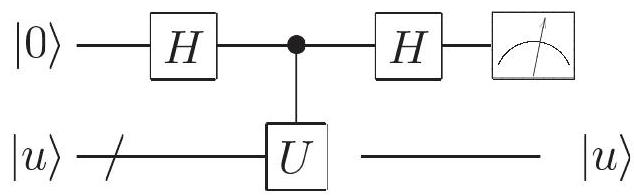
\includegraphics[width=0.75\linewidth]{Images/2024_05_17_6977ce60de6fd27aef98g-277}
\end{figure}

where $|u\rangle$ is an eigenstate of $U$ with eigenvalue $e^{2 \pi i \varphi}$. Show that the top qubit is\\
measured to be 0 with probability $p \equiv \cos ^{2}(\pi \varphi)$. Since the state $|u\rangle$ is unaffected by the circuit it may be reused; if $U$ can be replaced by $U^{k}$, where $k$ is an arbitrary integer under your control, show that by repeating this circuit and increasing $k$ appropriately, you can efficiently obtain as many bits of $p$ as desired, and thus, of $\varphi$. This is an alternative to the phase estimation algorithm.

Problem 5.4: The runtime bound $O\left(L^{3}\right)$ we have given for the factoring algorithm is not tight. Show that a better upper bound of $O\left(L^{2} \log L \log \log L\right)$ operations can be achieved.

Problem 5.5: (Non-Abelian hidden subgroups - Research) Let $f$ be a function on a finite group $G$ to an arbitrary finite range $X$, which is promised to be constant and distinct on distinct left cosets of a subgroup $K$. Start with the state

\begin{equation}
    \frac{1}{\sqrt{|G|^{m}}} \sum_{g_{1}, \ldots, g_{m}}\left|g_{1}, \ldots, g_{m}\right\rangle\left|f\left(g_{1}\right), \ldots, f\left(g_{m}\right)\right\rangle \tag{5.80}
\end{equation}

and prove that picking $m=4 \log |G|+2$ allows $K$ to be identified with probability at least $1-1 /|G|$. Note that $G$ does not necessarily have to be Abelian, and being able to perform a Fourier transform over $G$ is not required. This result shows that one can produce (using only $O(\log |G|)$ oracle calls) a final result in which the pure state outcomes corresponding to different possible hidden subgroups are nearly orthogonal. However, it is unknown whether a POVM exists or not which allows the hidden subgroup to be identified efficiently (i.e. using poly $(\log |G|)$ operations) from this final state.

Problem 5.6: (Addition by Fourier transforms) Consider the task of constructing a quantum circuit to compute $|x\rangle \rightarrow\left|x+y \bmod 2^{n}\right\rangle$, where $y$ is a fixed constant, and $0 \leq x<2^{n}$. Show that one efficient way to do this, for values of $y$ such as 1, is to first perform a quantum Fourier transform, then to apply single qubit phase shifts, then an inverse Fourier transform. What values of $y$ can be added easily this way, and how many operations are required?

Summary of Chapter 5: The quantum Fourier transform and its applications

\begin{itemize}
    \item When $N=2^{n}$ the quantum Fourier transform
\end{itemize}

\begin{equation}
    |j\rangle=\left|j_{1}, \ldots, j_{n}\right\rangle \longrightarrow \frac{1}{\sqrt{N}} \sum_{k=0}^{N-1} e^{2 \pi i \frac{i k}{N}}|k\rangle \tag{5.81}
\end{equation}

may be written in the form

\begin{equation}
    |j\rangle \rightarrow \frac{1}{2^{n / 2}}\left(|0\rangle+e^{2 \pi i 0 \cdot j_{n}}|1\rangle\right)\left(|0\rangle+e^{2 \pi i 0 \cdot j_{n-1} j_{n}}|1\rangle\right) \ldots\left(|0\rangle+e^{2 \pi i 0 \cdot j_{1} j_{2} \ldots j_{n}}|1\rangle\right) \tag{5.82}
\end{equation}

and may be implemented using $\Theta\left(n^{2}\right)$ gates.

\begin{itemize}
    \item Phase estimation: Let $|u\rangle$ be an eigenstate of the operator $U$ with eigenvalue $e^{2 \pi i \varphi}$. Starting from the initial state $|0\rangle^{\otimes t}|u\rangle$, and given the ability to efficiently perform $U^{2^{k}}$ for integer $k$, this algorithm (shown in Figure 5.3) can be used to efficiently obtain the state $|\tilde{\varphi}\rangle|u\rangle$, where $\tilde{\varphi}$ accurately approximates $\varphi$ to $t-$ $\left\lceil\log \left(2+\frac{1}{2 \epsilon}\right)\right\rceil$ bits with probability at least $1-\epsilon$.
    \item Order-finding: The order of $x$ modulo $N$ is the least positive integer $r$ such that $x^{r} \bmod N=1$. This number can be computed in $O\left(L^{3}\right)$ operations using the quantum phase estimation algorithm, for $L$-bit integers $x$ and $N$.
    \item Factoring: The prime factors of an $L$-bit integer $N$ can be determined in $O\left(L^{3}\right)$ operations by reducing this problem to finding the order of a random number $x$ co-prime with $N$.
    \item Hidden subgroup problem: All the known fast quantum algorithms can be described as solving the following problem: Let $f$ be a function from a finitely generated group $G$ to a finite set $X$ such that $f$ is constant on the cosets of a subgroup $K$, and distinct on each coset. Given a quantum black box for performing the unitary transform $U|g\rangle|h\rangle=|g\rangle|h \oplus f(g)\rangle$, for $g \in G$ and $h \in X$, find a generating set for $K$.
\end{itemize}

\section{History and Further Reading}
The definition of the Fourier transform may be generalized beyond what we have considered in this chapter. In the general scenario a Fourier transform is defined on a set of complex numbers $\alpha_{g}$, where the index $g$ is chosen from some group, $G$. In this chapter we have chosen $G$ to be the additive group of integers modulo $2^{n}$, often denoted $\mathbf{Z}_{2^{n}}$. Deutsch ${ }^{[\text {Deu85] }}$ showed that the Fourier transform over the group $\mathbf{Z}_{2}^{n}$ could be implemented efficiently on a quantum computer - this is the Hadamard transform of earlier chapters. Shor ${ }^{[S h o 94]}$ realized to spectacular effect that quantum computers could efficiently implement the quantum Fourier transform over groups $\mathbf{Z}_{m}$ for certain special values of $m$. Inspired by this result Coppersmith ${ }^{[\text {Coppy] }}$, Deutsch (unpublished), and Cleve (unpublished) gave the simple quantum circuits for computing the quantum Fourier transform over $\mathbf{Z}_{2^{n}}$ which we have used in this chapter. Cleve, Ekert, Mac-\\
chiavello and Mosca[CEMM98] and Griffiths and $\mathrm{Niu}^{[\mathrm{GN} 96]}$ independently discovered the product formula (5.4); in fact, this result had been realized much earlier by Danielson and Lanczos. The simplified proof starting in Equation (5.5) was suggested by Zhou. Griffiths and Niu ${ }^{[G N 96]}$ are responsible for the measured quantum Fourier transform found in Problem 5.2.

The Fourier transform over $\mathbf{Z}_{2^{n}}$ was generalized to obtain a Fourier transform over an arbitrary finite Abelian group by $\mathrm{Kitaev}^{[\mathrm{Kit} 95]}$, who also introduced the phase estimation procedure in the form given in Problem 5.3. Cleve, Ekert, Macchiavello and Mosca ${ }^{[C E M M 98]}$ also integrated several of the techniques of Shor and Kitaev into one nice picture, upon which Section 5.2 is based. A good description of the phase estimation algorithm can be found in Mosca's Ph.D. thesis ${ }^{[\text {Mos999] }}$.

Shor announced the quantum order-finding algorithm in a seminal paper in 1994 [Sho94], and noted that the problems of performing discrete logarithms and factoring could be reduced to order-finding. The final paper, including extended discussion and references, was published in $1997^{[\text {Sho } 07]}$. This paper also contains a discussion of clever multiplication methods that may be used to speed up the algorithm even further than in our description, which uses relatively naive multiplication techniques. With these faster multiplication methods the resources required to factor a composite integer $n$ scale as $O\left(n^{2} \log n \log \log n\right)$, as claimed in the introduction to the chapter. In $1995 \mathrm{Kitaev}^{[\mathrm{Kit} 95]}$ announced an algorithm for finding the stabilizer of a general Abelian group, which he showed could be used to solve discrete logarithm and factoring as special cases. In addition, this algorithm contained several elements not present in Shor's algorithm. A good review of the factoring algorithm was written by Ekert and Jozsa [E]96]; also see DiVincenzo [DiV95a]. The discussion of continued fractions is based upon Chapter 10 of Hardy and Wright ${ }^{[H W 60]}$. At the time of writing, the most efficient classical algorithm for factoring on a classical computer is the number field sieve. This is described in a collection edited by A. K. Lenstra and H. W. Lenstra, Jr.[LL93].

The generalization of quantum algorithms to solving the hidden subgroup problem has been considered by many authors. Historically, Simon was first to note that a quantum computer could find a hidden period of a function satisfying $f(x \oplus s)=f(x)^{[S i m 94, ~ S i m 97]}$. In fact, Shor found his result by generalizing Simon's result, and by applying a Fourier transform over $\mathbf{Z}_{N}$ instead of Simon's Hadamard transforms (a Fourier transform over $\mathbf{Z}_{2}^{k}$ ). Boneh and Lipton then noted the connection to the hidden subgroup problem, and described a quantum algorithm for solving the hidden linear function problem ${ }^{[B L 95]}$. Jozsa was the first to explicitly provide a uniform description of the Deutsch-Jozsa, Simon, and Shor algorithms in terms of the hidden subgroup problem ${ }^{[J o z 97]}$. Ekert and Jozsa's work in studying the role of the Abelian and non-Abelian Fast Fourier Transform algorithms in speedup of quantum algorithms $\mathrm{s}^{[\mathrm{E}] 98]}$ has also been insightful. Our description of the hidden subgroup problem in Section 5.4 follows the framework of Mosca and Ekert ${ }^{[\text {ME99, Mos99] }}$. Cleve has proven that the problem of finding an order of a permutation requires an exponential number of queries for a bounded-error probabilistic classical computer ${ }^{[\text {Cle99] }}$. Generalizations of this method to beyond Abelian groups have been attempted by Ettinger and Hoyer ${ }^{[\mathrm{EH} 99]}$, by Roetteler and Beth ${ }^{[\mathrm{RB} 98]}$ and Pueschel, Roetteler, and Beth ${ }^{[\text {PRB98] }}$, by Beals, who also described constructions of quantum Fourier

\begin{figure}
\centering
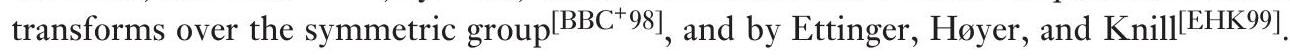
\includegraphics[width=0.75\textwidth]{Images/2024_05_17_6977ce60de6fd27aef98g-280}
\end{figure}

These results have shown, so far, that there exists a quantum algorithm to solve the hidden subgroup problem for non-Abelian groups using only $O(\log |G|)$ oracle calls, but whether this can be realized in polynomial time is unknown (Problem 5.5).


    % 有待整理

\chapter{Quantum Search Algorithms}
% 本章内容整理了NCBOOK的“6 Quantum search algorithms”,并增添原书没有的很多细节。
% 有待整理

%----------------------------------------------------------------------------------------
%	PART IV Notes of Papers
%----------------------------------------------------------------------------------------

\part{Notes of Papers}
% 大家平时阅读的一些有启发性的论文的笔记。主要是一些Variational Quantum Algorithms和QAOA的论文的笔记
% 本part的每一章就对应一篇论文。

\chapter{An Introduction to Variational Quantum Algorithms for Combinatorial Optimization Problems}
"An introduction to variational quantum algorithms for combinatorial optimization problems" \cite{grange2023introduction}

\vspace{10pt}

Variational Quantum Algorithms are heuristic algorithms that alternate between a quantum circuit and a classical optimizer. They tackle optimization problems of the form
\begin{equation}
    \min _{x \in\{0,1\}^n} f(x), \tag{1}
\end{equation}
where $f$ is any function defined on $\{0,1\}^n$. 

\section{Basics of Quantum Computing for Combinatorial Optimization}

\subsection{Quantum Bits \& Quantum Gates}

\begin{definition}[Canonical basis]
    The canonical basis of an $n$-qubit state is the set
\begin{equation}
    \mathcal{CB}_{n}=
\left\{\bigotimes_{k=1}^{n}\left|i^{(k)}\right\rangle,\left(i^{(1)}, \ldots, i^{(n)}\right) \in\{0,1\}^{n}\right\}
\end{equation}
where $i^{(k)}$ represents the state of the $k$-th qubit and $\otimes$ is the tensor product. For more readability, we omit to write the tensor product between qubits, i.e.,
\begin{equation}
    \mathcal{C B}_{n}=\left\{|i\rangle, i \in\{0,1\}^{n}\right\}.
\end{equation}
\end{definition}

The canonical basis is the set of all possible combinations of tensor products of $n$ one-qubit basis states, $|0\rangle$ and $|1\rangle$. Thus, in the matrix representation, each canonical basis state is a column vector of $2^{n}$ components with one component equal to 1 and the rest equal to 0. It directly results that the size of the canonical basis of an $n$-qubit state is $2^{n}$. 

% reversible %可逆的,相当于数学用语inverse, invertible

% $\left|\Phi^{+}\right\rangle=\frac{|00\rangle+|11\rangle}{\sqrt{2}}$

\subsection{Quantum Circuits}

In the circuit representation, qubits are numbered \textit{in ascending order from top to bottom} which is important for the tensor product circuit representation that follows. % 注意从电路图上看,composition的顺序是从左边到右边,而tensor的顺序是从上边到下边。这两类操作都是不可交换的操作,所以顺序很重要。

\subsubsection{Manipulate Quantum Gates to Build Other Quantum Gates}

We can manipulate quantum gates to build other quantum gates in two different ways. 
\begin{enumerate}
    \item The first one is the \textit{composition}. The composition of gates only operates between gates acting on the same qubits. 
\begin{figure}[ht]
    \centering
    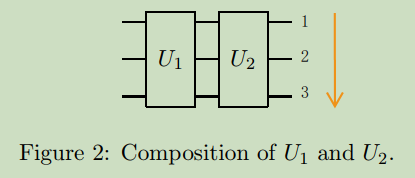
\includegraphics[width=0.5\linewidth]{Images/grange2023-1.png}
\end{figure}
    \item The other one is the \textit{tensor product}. The tensor product of gates can operates between gates acting on different qubits. Suppose $U_{1} \in \mathcal{M}_{2^{k}}(\mathbb{C})$ applies on the first $k$ qubits and $U_{2} \in \mathcal{M}_{2^{k^{\prime}}}(\mathbb{C})$ applies on the $k^{\prime}$ following ones. Their tensor product is the application of $U_{1}$ and $U_{2}$ on respective qubits in parallel. The matrix representation of this tensor product is $U_{1} \otimes U_{2}$. 
\begin{figure}[ht]
    \centering
    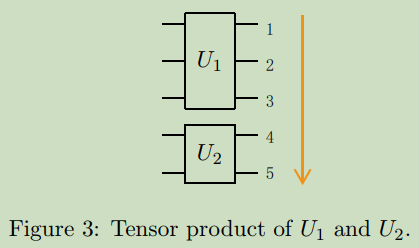
\includegraphics[width=0.5\linewidth]{Images/grange2023-2.png}
\end{figure}
\end{enumerate}
One readily verifies that both composition and tensor product transform unitary matrices into a resulting unitary matrix.

Notice that when we apply a quantum gate on $k$ qubits of an $n$-qubit system, it supposes that we apply identity gate $I$ on the qubits not concerned. 

\begin{example}
For instance, let us consider a 3-qubit system on which we apply $U \in \mathcal{M}_{2}(\mathbb{C})$ on qubit number 2. The matrix representation of the resulting 3-qubit gate is $I \otimes U \otimes I$, and its circuit representation is illustrated on Fig.4, where the application of $I$ is usually replaced by a simple wire.
\begin{figure}[ht]
    \centering
    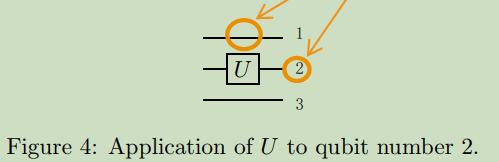
\includegraphics[width=0.5\linewidth]{Images/grange2023-3.png}
\end{figure}
\end{example}

\subsubsection{What is a Quantum Algorithm?}

Throughout, we consider that \textit{a quantum algorithm is a quantum circuit acting on $n$ qubits, that is, a sequence of quantum gates' compositions and/or tensor products. } % 概括得挺好

These quantum gates can be $k$-qubit gates, for $k \in[n]$. % k是小于等于n的整数。相对于很大n,当k足够小时,k-qubit gates 就可以称之为 small gates。

However, quantum gates involving many qubits are typically not implementable natively on quantum computers and need to be decomposed into smaller and simpler gates. This set of small gates can be considered as the quantum counterpart of the elementary logic gates used in classical circuit computing to assess \textit{the circuit complexity} of a classical algorithm. % 也就是说电路的复杂度可以由构成其的基础gates的个数来做衡量,这一想法是来自于经典电路的。

Thus, an $n$-qubit quantum algorithm is described by a unitary matrix in $\mathcal{M}_{2^{n}}(\mathbb{C})$, and we decompose it as a sequence of universal gates to obtain the \textit{complexity of the quantum algorithm}. % 也就是说量子电路的复杂度可以由构成其的基础量子gates的个数来做衡量

\subsubsection{Universal Gates}

\begin{definition}[Set of universal gates]
    A set of quantum gates PU is \textit{universal} if we can decompose any $n$-qubit quantum gate through a circuit composed solely of the gates in PU.
\end{definition}

\begin{remark}
\begin{itemize}
    \item In definition above, we implicitly allow PU to be a set of infinite elements (countable or uncountable). Of course, we want PU to be small as soon as possible.
    \item In definition above, the word "composed" contains both the composition operations and tensor product operations.
    \item Note that this "decompose" is exact decomposition, and there no error.
\end{itemize}
\end{remark}

Fortunately, there exist different universal sets of quantum gates. We introduce below such a set formed of four types of gates. 

\begin{example}[Some important small gates]
First, we consider the three following families of one-qubit gates, each of which is parametrized by a real number $\theta \in \mathbb{R}$:
\begin{align}
& R_{X}(\theta)=\left(\begin{array}{cc}
\cos \frac{\theta}{2} & -i \sin \frac{\theta}{2} \\
-i \sin \frac{\theta}{2} & \cos \frac{\theta}{2}
\end{array}\right)  \tag{5}\\
& R_{Y}(\theta)=\left(\begin{array}{cc}
\cos \frac{\theta}{2} & -\sin \frac{\theta}{2} \\
\sin \frac{\theta}{2} & \cos \frac{\theta}{2}
\end{array}\right)  \tag{6}\\
& R_{Z}(\theta)=\left(\begin{array}{cc}
e^{-i \frac{\theta}{2}} & 0 \\
0 & e^{i \frac{\theta}{2}}
\end{array}\right) \tag{7}
\end{align}
Second, we consider the two-qubit gate CX (or, CNOT, Controlled Not, Controlled X gate):
\begin{equation}
    C X=\left(\begin{array}{llll}
1 & 0 & 0 & 0  \tag{8}\\
0 & 1 & 0 & 0 \\
0 & 0 & 0 & 1 \\
0 & 0 & 1 & 0
\end{array}\right)
\end{equation}
In other words, we can define $C X$ on the canonical basis as
\begin{equation}
    C X|a, b\rangle=|a, b \oplus a\rangle
\end{equation}
for $a, b \in\{0,1\}$, where $\oplus$ is the addition modulo 2 .
\end{example}

\begin{remark}[Notation on gates indexes]
Henceforth, we use the notation $R_{X, i}$ for the application of $R_{X}$ on qubit $i$ (and the application of identity matrix on the remaining qubits). We do the same with $R_{Y, i}$ and $R_{Z, i}$. 
% 这一中比较偷懒的写法:$R_{X, i}$,可以用来表示一个非常大的gates,但其中只有第i个qubit是受到非平凡的$R_{X}$的操作。这类写法在其他文献中也经常使用。
We note $C X_{i, j}$ the application of $C X$ gate to qubits $i$ and $j$: $X$ is applied to qubit $j$ if and only if qubit $i$ is in state $|1\rangle$.
% 明确标记控制位i和操作位j也是CX门常见写法。但有时不同文献会有细微差别,要注意别混淆。
\end{remark}

\begin{theorem}[Universal gates \cite{nielsen2010quantum}]
We claim that
\begin{itemize}
    \item The set of all one-qubit gates and the $C X$ gate is universal.
    \item Any one-qubit gate is the composition of rotation gates (5)-(7).
    \item Thus, the set 
\begin{equation}
    P U=\left\{R_{X}(\alpha), R_{Y}(\beta), R_{Z}(\gamma), C X: \alpha, \beta, \gamma \in \mathbb{R}\right\}
\end{equation}
is also universal.
\end{itemize}
\end{theorem}

In comparison, the sets of gates $\{N A N D\},\{N O R\},\{N O T, A N D\}$ and $\{N O T, O R\}$ are universal for classical computation. \todo{Need proof.} Indeed, we can compute any arbitrary classical function with them. % 这一部分知识是传统计算科学里出现的证明,未来有时间好好研究一下。

In view of the above, we typically consider that the quantum counterpart of the classical number of elementary operations is the number of universal gates used to decompose the circuit. Of course, this decomposition depends on the set of universal gates $P U$ considered, but the number of gates required is the same with any set, modulo a multiplicative constant. 

% Thereafter, we only consider the set $P U$ defined in Theorem 13. This choice is motivated by the algorithms we study in this paper, as it will be convenient to express them with this set. 

Furthermore, if we consider the family of circuits $\left(\mathcal{C}_{n}\right)_{n \in \mathbb{N}}$ where $\mathcal{C}_{n}$ is a circuit on $n$ qubits and is decomposed on $\mathcal{O}(\operatorname{poly}(n))$ universal quantum gates, then this family is said to be \textit{efficient}.

\subsection{Non-classical Behaviors} % 确实,前面几节没有让人感觉奇怪的设定。作者把量子特有的设定放在一起,以区别经典行为。这一思路值得借鉴。

The quantum algorithms rely on three characteristics of quantum states with no classical equivalent: measurement, superposition, and entanglement.

\subsubsection{Measurement} %该论文的测量介绍,把很艰难晦涩的测量,用短短的语言就清晰地刻画了。很值得学习。他不涉及各种可观测量,投影算子,POVM等复杂概念。

We need to measure a quantum state $|\psi\rangle$ to get information from it; otherwise, no information is accessible.
Moreover, it only extracts partial information from the quantum state at once measurement: the single measurement output of  $|\psi\rangle$ is a bitstring\footnote{$n$-bitstring is the element of $\{0,1\}^{n}$}.

\begin{definition}[Measurement]
    In the gate-based quantum model, the measurement $\mathcal{M}$ of an $n$-qubit state $|\psi\rangle=\sum_{i \in\{0,1\}^{n}} \psi_{i}|i\rangle$ outputs the $n$-bitstring $i$ with probability $\left|\psi_{i}\right|^{2}$. After having been measured, state $|\psi\rangle$ no longer exists: it has been replaced by the state $|i\rangle$.
\end{definition}

\begin{example}
    For example, measuring qubit $|q\rangle=q_{0}|0\rangle+q_{1}|1\rangle$ outputs 0 with probability $\left|q_{0}\right|^{2}$ and 1 with probability $\left|q_{1}\right|^{2}$, and changes the state $|q\rangle$ to $|0\rangle$ and $|1\rangle$, respectively.  % 这个例子值得玩味的点是,我们测量得到的结果outcome是label(用bitstring表示),而原量子态坍缩成对应的label的basis state。所以,不应该说,测量得到的结果就是basis state自身。
\end{example}

Some points:
\begin{itemize}
    \item A measurement appears as a loss of information. Indeed, we describe an $n$-qubit state by $2^{n}$ normalized complex coefficients, but we only extract an $n$-bitstring after measuring it.
    \item The perfect knowledge of the probabilities representing a given quantum state $|\psi\rangle$, namely, the square module of each of its coordinates 
    \begin{equation}
    \left(\left|\psi_{i}\right|^{2}\right)_{i \in\{0,1\}^{n}} \in[0,1]^{2^{n}},
\end{equation}
can be obtained \textit{only if we measure $|\psi\rangle$ an infinite number of times.} Notice that it requires resetting state $|\psi\rangle$ after each measurement.
    \item Note that we never get the exact complex numbers $\psi_{i}$, instead of, their squared module $\left|\psi_{i}\right|^{2}$ at most.
    \item Different qubit state might have the same probabilities representing.
\end{itemize}

In reality we are limited to approximating a given quantum state through sampling. In particular, if $|\psi\rangle$ is the result of an algorithm, this means we have to repeat the same algorithm for every measurement of $|\psi\rangle$ we wish to perform.

\subsubsection{Superposition}

\begin{definition}[Superposition]
    A quantum state $|\psi\rangle$ is said in superposition if $|\psi\rangle=$ $\sum_{i \in\{0,1\}^{n}} \psi_{i}|i\rangle$ where there are \textit{at least two terms }with non-zero coefficients in the sum. Equivalently, a quantum state that is not a basis state is in superposition.
\end{definition}

\begin{remark}
    \begin{itemize}
    \item A quantum state is in superposition. = A quantum state is superposed.
    \item A quantum stated superposed is $\dots$
    \end{itemize}
\end{remark}

The Hadamard gate $H=\frac{1}{\sqrt{2}}\left(\begin{array}{cc}1 & 1 \\ 1 & -1\end{array}\right)$ is essential in quantum computing because it creates superposition starting from a basis state. We obtain the state $|+\rangle$, respectively $|-\rangle$, by applying $H$ on $|0\rangle$, respectively $|1\rangle:$
\begin{equation}
\begin{aligned}
& H|0\rangle=\frac{|0\rangle+|1\rangle}{\sqrt{2}}=:|+\rangle \\
& H|1\rangle=\frac{|0\rangle-|1\rangle}{\sqrt{2}}=:|-\rangle
\end{aligned}
\end{equation}
The two states $|+\rangle$ and $|-\rangle$ are in uniform superposition because both have the same probability of being measured as 0 or 1.

\begin{definition}[uniformly superposition]
    In general, an $n$-qubit state is in uniformly superposition if it is equal to 
\begin{equation}
    \frac{1}{\sqrt{2^{n}}} \sum_{j \in\{0,1\}^{n}} e^{i \alpha_{j}}|j\rangle,
\end{equation}
with $\alpha_{j} \in\left[0,2 \pi\left[, \forall j \in\{0,1\}^{n}\right.\right.$. % 注意,uniform的含义不是非要各个系数自身相等,而是他们的modulus相等。下面的$|+\rangle^{\otimes n}$ 提供一种各个系数自身相等的特殊情况。
In what follows, we shall often use the following uniformly superposed $n$-qubit state 
\begin{equation}
    |+\rangle^{\otimes n}=\frac{1}{\sqrt{2^{n}}} \sum_{i \in\{0,1\}^{n}}|i\rangle.
\end{equation}
\end{definition}

\begin{remark} 
Some points in definition above:
    \begin{itemize}
    \item $[0,2 \pi[$ means $[0,2 \pi)$.
    \item Sometimes, we need carefully distinguish "index $i$ " with "pure imaginary number $i$". 
    \end{itemize}
\end{remark}

When applying the tensor product of $n$ Hadamard gates, each applied to a qubit initially in state $|0\rangle$, specifically
\begin{equation}
    H^{\otimes n}|0\rangle^{\otimes n}=\bigotimes_{i=1}^{n} H|0\rangle=\bigotimes_{i=1}^{n}\left(\frac{|0\rangle+|1\rangle}{\sqrt{2}}\right)=\frac{1}{\sqrt{2^{n}}} \sum_{i \in\{0,1\}^{n}}|i\rangle=|+\rangle^{\otimes n}. \tag{9}
\end{equation}
In the left first equality, we used the following relation
\begin{equation}
    (A \otimes B)(C \otimes D)=(A C \otimes B D).
\end{equation}
Equation (9) illustrates the potential benefit of quantum circuits: applying $\mathcal{O}(n)$ universal one-qubit gates impacts the exponentially many coefficients of $|\psi\rangle$. Indeed, one readily verifies that 
\begin{equation}
    H=R_{X}(\pi) R_{Y}\left(\frac{\pi}{2}\right)
\end{equation}
modulo a global phase, so $H^{\otimes n}$ amounts to applying $2 n$ universal one-qubit gates.

\begin{remark}
    Two quantum states $|\psi\rangle$ and $\left|\psi^{\prime}\right\rangle=e^{i \alpha}|\psi\rangle$, with $\alpha \in[0,2 \pi[$, that only differ by a global phase are indiscernible by measurement. Thus, \textit{we do not consider global phase of quantum states nor quantum gates.} % 无论是gate还是state,如果只相差一个modulu 为1的复数因子,我们都不区分它们,而把他们当作一个东西。
\end{remark}

\subsubsection{Entanglement}

Entanglement has the peculiar and helpful property that we can apply a circuit only on a part of the $n$-qubit system, and as a result, the whole system is affected.

\begin{definition}[Product state]
    An $n$-qubit state is a product state if it is the tensor product of $n$ one-qubit states. In other words, an $n$-qubit state $|\psi\rangle$ is a product state if it exists $2 n$ complex coefficients $\left(q_{0}^{(j)}, q_{1}^{(j)}\right)_{j \in[n]}$ such that
\begin{equation}
    |\psi\rangle=\bigotimes_{j=1}^{n}\left(q_{0}^{(j)}|0\rangle+q_{1}^{(j)}|1\rangle\right), \text { with }\left|q_{0}^{(j)}\right|^{2}+\left|q_{1}^{(j)}\right|^{2}=1, \forall j \in[n].
\end{equation}
Thus, each state of a qubit that composes $|\psi\rangle$ can be described independently of the states of the other.
\end{definition}

\begin{definition}[Entangled state]
    An $n$-qubit state $|\psi\rangle=\sum_{i \in\{0,1\}^{n}} \psi_{i}|i\rangle$ is entangled if the numerical values of its coordinates $\left(\psi_{i}\right)_{i \in\{0,1\}^{n}} \in \mathbb{C}^{2^{n}}$ admit no solution $\left(q_{0}^{(j)}, q_{1}^{(j)}\right)_{j \in[n]} \in \mathbb{C}^{2 n}$ to the system
\begin{equation}
    \left\{\begin{array}{l}
\sum_{i \in\{0,1\}^{n}} \psi_{i}|i\rangle=\bigotimes_{j=1}^{n}\left(q_{0}^{(j)}|0\rangle+q_{1}^{(j)}|1\rangle\right) \\
\left|q_{0}^{(j)}\right|^{2}+\left|q_{1}^{(j)}\right|^{2}=1, \forall j \in [n]
\end{array}\right.
\end{equation}

\end{definition}

If an $n$-qubit state is not a product state, it is an entangled state. Operations performed on some coordinates of the entangled state can affect the other coordinates without direct operations on them.

\begin{remark}
    \begin{itemize}
    \item Each quantum state is either a product state or an entangled state.
    \item Each quantum state is either a basis state or a superposed state.
    \item There is a difference between superposition and entanglement, but there are some implication relation between those concepts, see next figure. % 但又有一些关联
\begin{figure}[ht]
    \centering
    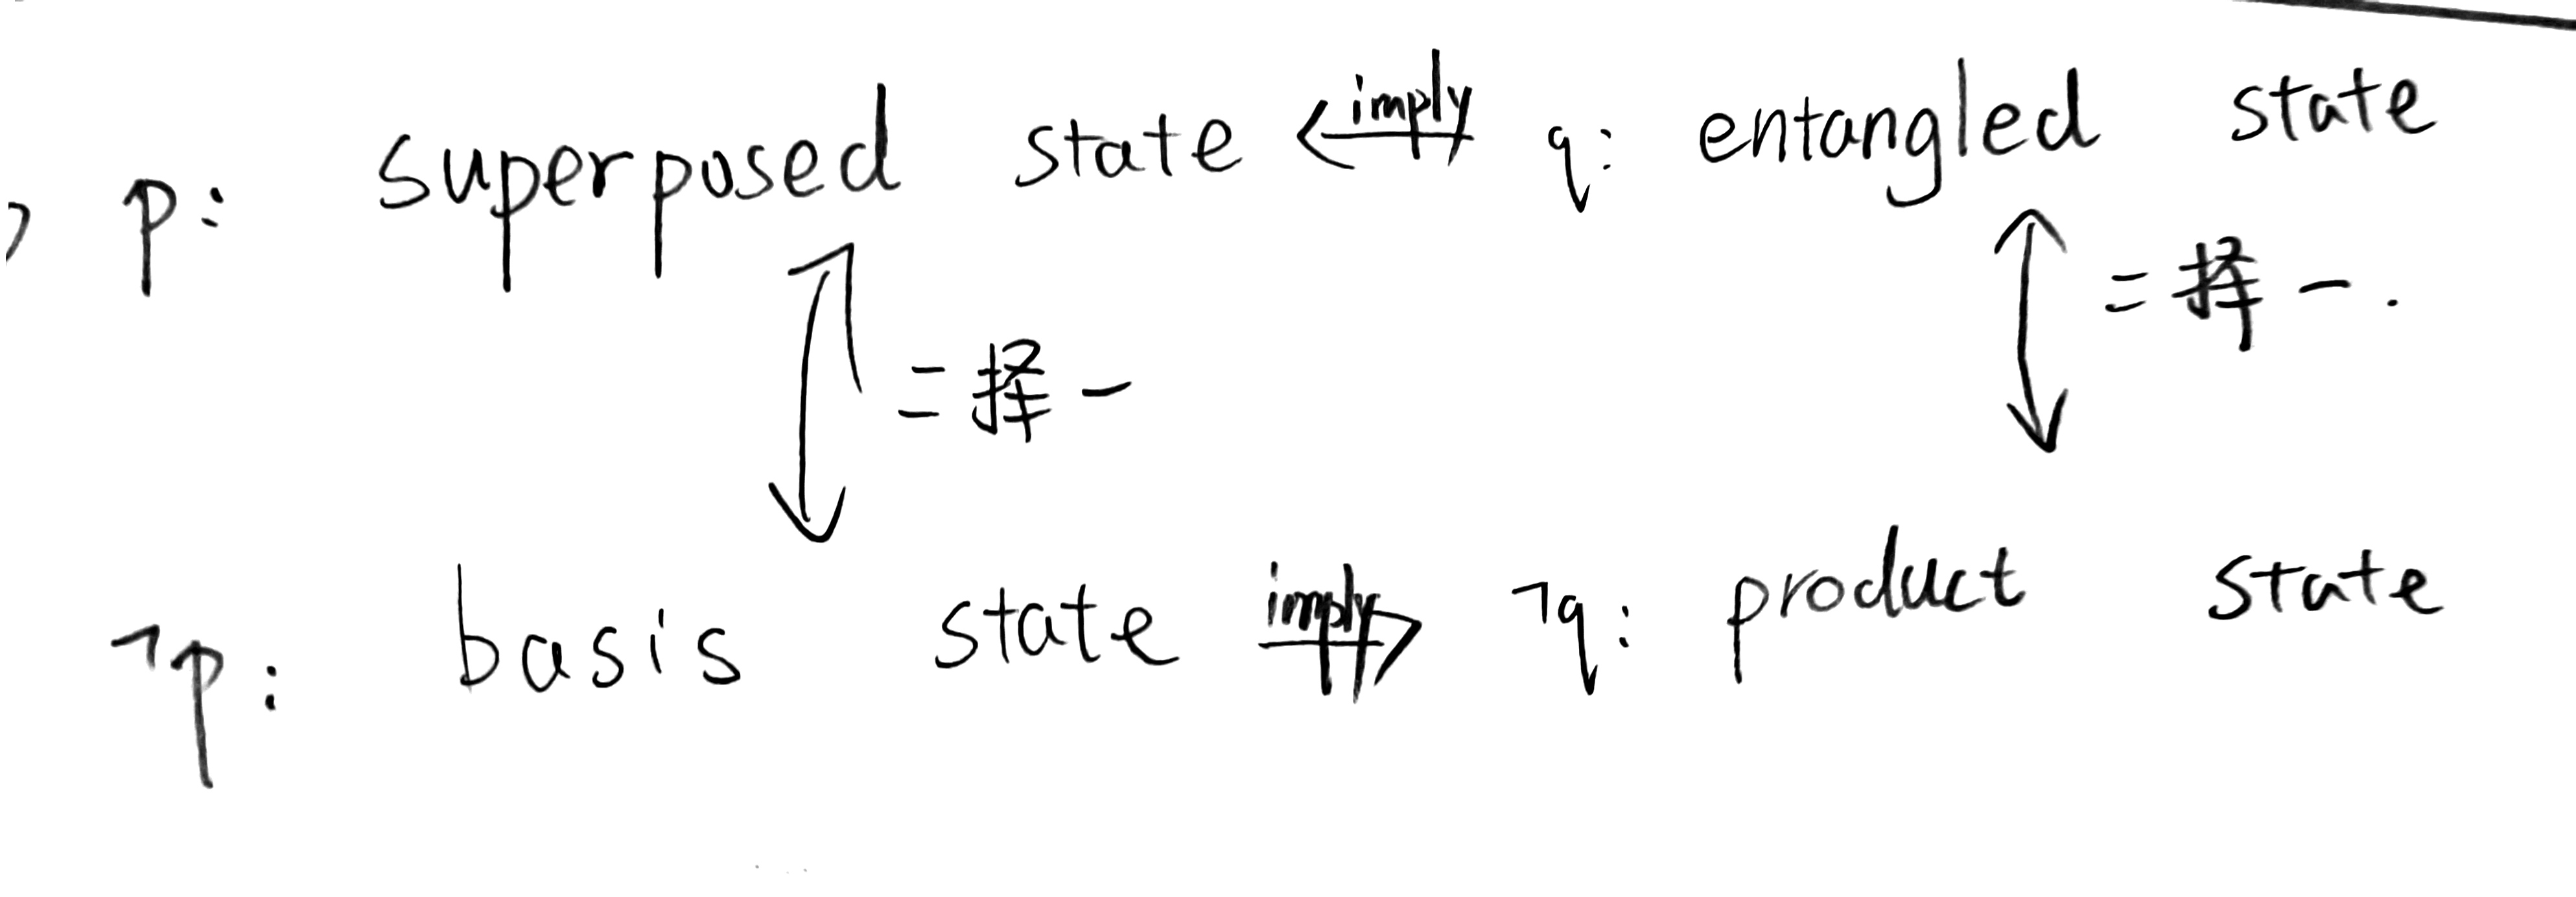
\includegraphics[width=0.75\linewidth]{Images/relation-superposed-entangled.jpg}
\end{figure}
    \item Notice that when an $n$-qubit system is entangled, it makes no sense to speak about qubit number $k \in[n]$ because isolated qubits are not defined. 
    \end{itemize}
\end{remark}

\section{Variational Quantum Algorithms for Optimization}

Some of the quantum algorithms that tackle combinatorial optimization problems are Variational\footnote{The word "variational" does not have that mathematical meaning.} Quantum Algorithms (VQAs). They are hybrid algorithms because they require both quantum and classical computations. 

VQAs are studied today because they represent an alternative approach that reduces the quality and quantity of the quantum resources needed. Specifically, they are designed to run on the \textbf{NISQ era} where quantum computers are noisy with few qubits: for instance, they harness low-depth quantum circuits.

In this section, we consider optimization problems of the form
\begin{equation}
    \min _{x \in\{0,1\}^{n}} f(x), \tag{1}
\end{equation}
where $f$ is any function defined on $\{0,1\}^{n}$. We note $\mathcal{F}$ the set of optimal solutions.

\subsection{General Description}

Variational Quantum Algorithms (VQAs) are hybrid algorithms that, given an input $|0\rangle^{\otimes n}$, alternate between a quantum and a classical part. Henceforth, we note $\left|0_{n}\right\rangle$ the state $|0\rangle^{\otimes n}$ to ease the reading. 

Let us first provide a high-level description of the key elements of VQAs that are detailed in this section. Let $d \in \mathbb{N}$, the three key elements of VQAs are:
\begin{itemize}
    \item a \textbf{parametrized quantum circuit}, $U: \mathbb{R}^{d} \rightarrow \mathcal{M}_{2^{n}}(\mathbb{C})$,
    \item a \textbf{guiding function}, $g: \mathbb{R}^{d} \rightarrow \mathbb{R}$,
    \item and a \textbf{classical optimizer}, which is an algorithm $\mathcal{A}$ that optimizes $g$ over space $\mathbb{R}^{d}$.
\end{itemize}
Before that, we provide a general overview of VQAs in Algorithm 1. 
\begin{figure}[ht]
    \centering
    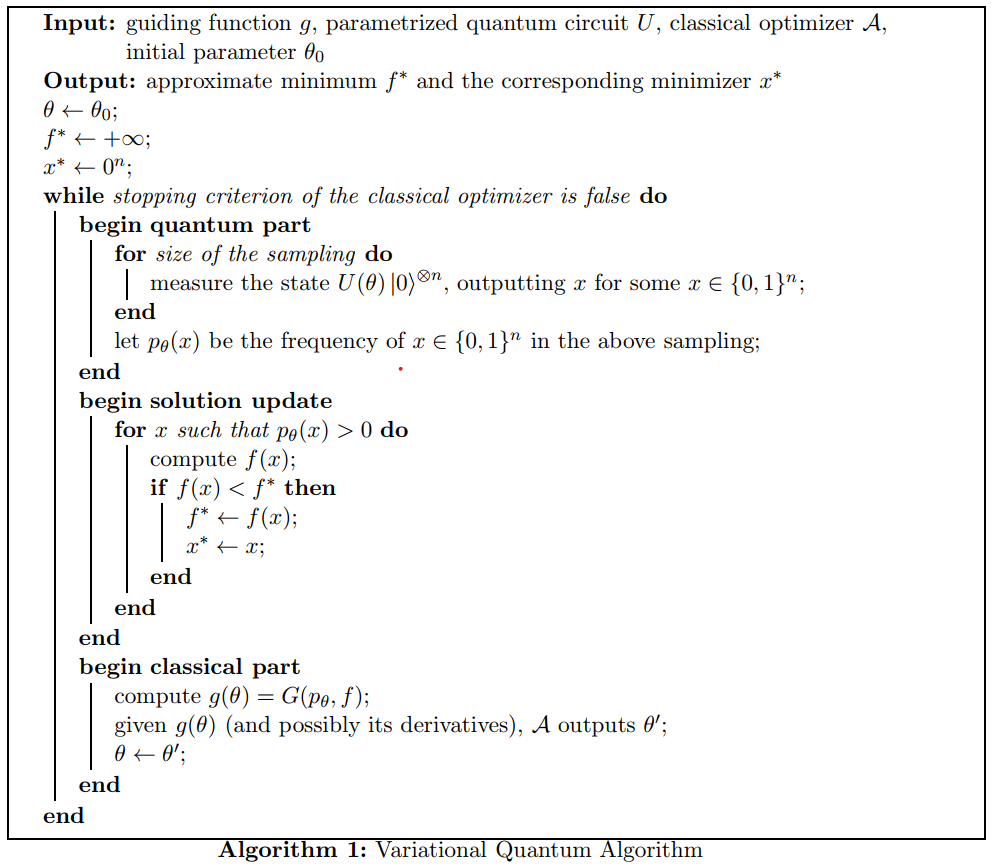
\includegraphics[width=1\linewidth]{Images/VQA-algorithm.png}
\end{figure}

The main idea of a VQA is as follows. The main loop of the algorithm executes the following steps until the classical optimizer stops according to a given stopping criterion. 

\begin{enumerate}
    \item \textbf{(Quantum part)} First, given $\theta \in \mathbb{R}^{d}$, the quantum part executes the parametrized quantum circuit $U(\theta)$ for several times to sample the quantum state. It results in a (discrete) distribution probability over $\{0,1\}^{n}$ that we note $\left\{p_{\theta}(x): x \in\{0,1\}^{n}\right\}$. % 应该是简单的频率frequency统计 % 理论上我们可以重复无数次实验,以获得该离散分布的全部信息。
    \item \textbf{(Classical part)} Second, the classical part computes the cost of this state, through the evaluation of the guiding function, according to the sampling results $p_{\theta}$, specifically, $g(\theta)=G\left(p_{\theta}, f\right)$ for a given function $G$ that is constructed from $f$ and $p_{\theta}$. For example, such $g$ can be
    \begin{equation}
    g(\theta)=\sum_{x \in\{0,1\}^n} p_\theta(x) f(x).
\end{equation}
    More precisely, for a given $\theta$, the computation of $G$ requires only the values $f(x)$ for $x$ such that $p_{\theta}(x)>0$. Eventually, this cost value is given to the classical optimizer $\mathcal{A}$, which outputs a new parameter in order to minimize $g$. % 可以用一些零阶优化技术 % Notice that, between the two parts the best-found solution is possibly updated by a classical computer.
\end{enumerate}

In the following subsections, we detail each part of VQAs and show \textbf{how specific choices of $g$ and $U$} \textbf{ensure that VQAs optimize $f$}.

\subsection{Quantum Part}

The quantum part of VQAs applies a quantum circuit on the $n$-qubit system that constitutes the quantum computer. Importantly, \textit{variational}\footnote{The word "variational" does not have that mathematical meaning.}  in VQAs stands for the parametrization of the quantum circuit. 

Let $d \in \mathbb{N}$ be the number of parameters, thus $\theta \in \mathbb{R}^d.$ A \textit{parametrized quantum circuit} is a continuous function $U: \mathbb{R}^{d} \rightarrow$ $\mathcal{M}_{2^{n}}(\mathbb{C})$ mapping any $\theta \in \mathbb{R}^{d}$ to unitary matrix $U(\theta)$.

As defined in Sect. 2.3, a quantum circuit is a sequence of universal quantum gates' compositions and/or tensor products. Thus, all coefficients of matrix $U(\theta)$ are continuous functions on $\mathbb{R}^{d}$.

\begin{example}
    A simple example of a parametrized quantum circuit for $n=3$ and $d=3$ is depicted in Fig. 6.
\begin{figure}[ht]
    \centering
    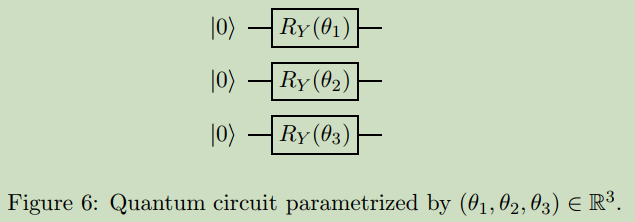
\includegraphics[width=0.75\linewidth]{Images/parametrized-quantum-circuit.png}
\end{figure}
The expression of $U(\theta)$ for this circuit is as follows: $\forall \theta=\left(\theta_1, \theta_2, \theta_3\right) \in \mathbb{R}^3$,
\begin{equation}
\begin{aligned}
& U(\theta)=R_Y\left(\theta_1\right) \otimes R_Y\left(\theta_2\right) \otimes R_Y\left(\theta_3\right) \\
& =\left(\begin{array}{cc}
\cos \frac{\theta_1}{2} & -\sin \frac{\theta_1}{2} \\
\sin \frac{\theta_1}{2} & \cos \frac{\theta_1}{2}
\end{array}\right) \otimes\left(\begin{array}{cc}
\cos \frac{\theta_2}{2} & -\sin \frac{\theta_2}{2} \\
\sin \frac{\theta_2}{2} & \cos \frac{\theta_2}{2}
\end{array}\right) \otimes\left(\begin{array}{cc}
\cos \frac{\theta_3}{2} & -\sin \frac{\theta_3}{2} \\
\sin \frac{\theta_3}{2} & \cos \frac{\theta_3}{2}
\end{array}\right) \\
& =\left(\begin{array}{cccccccc}
c_1 c_2 c_3 & -c_1 c_2 s_3 & -c_1 s_2 c_3 & c_1 s_2 s_3 & -s_1 c_2 c_3 & s_1 c_2 s_3 & s_1 s_2 c_3 & -s_1 s_2 s_3 \\
c_1 c_2 s_3 & c_1 c_2 c_3 & -c_1 s_2 s_3 & -c_1 s_2 c_3 & -s_1 c_2 s_3 & -s_1 c_2 c_3 & s_1 s_2 s_3 & s_1 s_2 c_3 \\
c_1 s_2 c_3 & -c_1 s_2 s_3 & c_1 c_2 c_3 & -c_1 c_2 s_3 & -s_1 s_2 c_3 & s_1 s_2 s_3 & -s_1 c_2 c_3 & s_1 c_2 s_3 \\
c_1 s_2 s_3 & c_1 s_2 c_3 & c_1 c_2 s_3 & c_1 c_2 c_3 & -s_1 s_2 s_3 & -s_1 s_2 c_3 & -s_1 c_2 s_3 & -s_1 c_2 c_3 \\
s_1 c_2 c_3 & -s_1 c_2 s_3 & -s_1 s_2 c_3 & s_1 s_2 s_3 & c_1 c_2 c_3 & -c_1 c_2 s_3 & -c_1 s_2 c_3 & c_1 s_2 s_3 \\
s_1 c_2 s_3 & s_1 c_2 c_3 & -s_1 s_2 s_3 & -s_1 s_2 c_3 & c_1 c_2 s_3 & c_1 c_2 c_3 & -c_1 s_2 s_3 & -c_1 s_2 c_3 \\
s_1 s_2 c_3 & -s_1 s_2 s_3 & s_1 c_2 c_3 & -s_1 c_2 s_3 & c_1 s_2 c_3 & -c_1 s_2 s_3 & c_1 c_2 c_3 & -c_1 c_2 s_3 \\
s_1 s_2 s_3 & s_1 s_2 c_3 & s_1 c_2 s_3 & s_1 c_2 c_3 & c_1 s_2 s_3 & c_1 s_2 c_3 & c_1 c_2 s_3 & c_1 c_2 c_3
\end{array}\right), \\
&
\end{aligned}
\end{equation}
where $c_i=\cos \frac{\theta_i}{2}$ and $s_i=\sin \frac{\theta_i}{2}$ for $i \in[3]$.
\end{example}

\subsection{Classical Part}

The classical part of VQAs consists of a classical optimization over the parameters $\theta \in \mathbb{R}^{d}$. 

\textbf{The classical optimizer essentially aims at finding the optimal parameters $\theta^{*}$ that lead to optimal solutions of the initial problem (1) with high probability}, specifically, such that
\begin{equation}
    \sum_{s \in \mathcal{F}}\left|\left\langle s\left|U\left(\theta^{*}\right)\right| 0_{n}\right\rangle\right|^{2} \geq 1-\epsilon \tag{10}
\end{equation}
for small $\epsilon>0$. 

\begin{remark}
    \begin{itemize}
    \item We note $\mathcal{F}$ the set of optimal solutions in problem (1). We allow $\mathcal{F}$ to contain many different optimal solutions.
    \item We note $\left|0_{n}\right\rangle$ the state $|0\rangle^{\otimes n}$ to ease the reading. Here, $0_{n}=000\dots0.$
    \item $U\left(\theta\right)| 0_{n}\rangle$ is the output state of the parametrized quantum circuit.
    \item Note that we encode each possible optimization of (1), i.e, the n-bitstring, to basis state of quantum state space.
    \item We use notation $|s\rangle$ instead of $|i\rangle$ to efficiently recall that we deal with solutions of optimization problems (1). In fact, $\mathcal{F} \subset \{0,1\}^{n}$ and we use $s$ to denote the elements of $\mathcal{F}.$
    \item In fact, we measure the output state by using the computational basis. In this paper, they are $\mathcal{C B}_{n}=\left\{|i\rangle, i \in\{0,1\}^{n}\right\}$.
    \item $\left|\left\langle s\left|U\left(\theta^*\right)\right| 0_n\right\rangle\right|^2$ is the probability with outcome $s$ after measurement. Then, $\sum_{s \in \mathcal{F}}\left|\left\langle s\left|U\left(\theta^{*}\right)\right| 0_{n}\right\rangle\right|^{2}$ is the probability with arbitrary optimal solutions after measurement.
    \end{itemize}
\end{remark}

The classical part is characterized by two aspects: 
\begin{enumerate}
    \item the function that guides the optimization
    \item the optimizer itself.
\end{enumerate}

\subsection{Guiding Function}

Let us denote 
\begin{equation}
    \mathcal{F}_{\text {quant }}=\left\{\sum_{s \in \mathcal{F}} \psi_{s}|s\rangle: \sum_{s \in \mathcal{F}}\left|\psi_{s}\right|^{2}=1\right\}
\end{equation}
as the set of quantum states that are superpositions of optimal solutions of problem (1). So if we measure any state in $\mathcal{F}_{\text {quant }}$, our result will be the optimal solution to the original optimization problem.

Let $g: \mathbb{R}^{d} \rightarrow \mathbb{R}$ be the guiding function, and $g$ acts as a link between the quantum and classical parts. \textbf{Naturally, we would like to define $g$ such that minimizing $g$ tends to minimize $f$.}

\begin{definition}[Guiding function]
    Let $g: \mathbb{R}^{d} \rightarrow \mathbb{R}$ be a function and $\mathcal{G}$ be its set of minimizers. We call $g$ \textit{a guiding function for $f$ with respect to $U$} if $g$ is continuous and
\begin{equation}
    \left\{U(\theta)\left|0_{n}\right\rangle: \theta \in \mathcal{G}\right\} \subseteq \mathcal{F}_{\text {quant}}. \tag{11}
\end{equation}
\end{definition}

\begin{itemize}
    \item Indeed, Equation (11) implies that measuring the quantum state $U\left(\theta\right)|0\rangle^{\otimes n}$ for any $\theta\in \mathcal{G}$ outputs with probability 1 an optimal solution of the initial problem $s \in \mathcal{F}$.
    \item In other words, optima of a guiding function $g$ must lead to optima of $f$ or superpositions of optima of $f$.
    \item Thus, minimizing $f$ amounts to minimizing $g$, and finding $\mathcal{F}$ is done by finding $\mathcal{G}$. The latter is found with the classical optimizer.
\end{itemize}

% 下面两个remark亟需解决!

\begin{remark}
    Without any information on $\mathcal{F}$, we need to choose a quantum circuit $U$ such that any optimal solution $s \in \mathcal{F}$ is reachable, specifically, we construct $U$ such that
\begin{equation}
    \left\{U(\theta)\left|0_{n}\right\rangle: \theta \in \mathbb{R}^{d}\right\} \supseteq \mathcal{C} \mathcal{B}_{n} \supseteq \mathcal{F}. \tag{12}
\end{equation}
Notice that this condition is weak and easily satisfied. For instance, the circuit depicted in Fig. 6 satisfies this condition. % 这段话暗示了,U的构造也需要精心设计的。
\end{remark}

\begin{remark}
If ever one is interested in finding all optimal solutions of problem (1), the circuit and the guiding function should satisfy instead the stronger condition than (11)
\begin{equation}
    \left\{U(\theta)\left|0_{n}\right\rangle: \theta \in \mathcal{G}\right\}=\mathcal{F}_{\text {quant}}. \tag{13}
\end{equation}
In that case, $U$ satisfying (12) is not enough. Without any information on $\mathcal{F}$, we need to choose $U$ that can reach any $n$-qubit quantum states, specifically, % 这段话暗示了,U的构造也需要精心设计的。
\begin{equation}
    \left\{U(\theta)\left|0_{n}\right\rangle: \theta \in \mathbb{R}^{d}\right\}=\left\{\sum_{x \in\{0,1\}^{n}} \psi_{x}|x\rangle: \sum_{x \in\{0,1\}^{n}}\left|\psi_{x}\right|^{2}=1\right\}
\end{equation}
% 上式右侧是全部整个quantum state space!
\end{remark}

\begin{definition}[Mean function]
A popular choice for the guiding function in the literature is the \textit{mean function}
\begin{equation}
    g_{\text {mean }}(\theta)=\sum_{x \in\{0,1\}^{n}} p_{\theta}(x) f(x), \tag{14}
\end{equation}
where
\begin{equation}
    p_{\theta}(x)=\left|\left\langle x|U(\theta)| 0_{n}\right\rangle\right|^{2}
\end{equation}
is the probability of finding $x$ when $U(\theta)\left|0_{n}\right\rangle$ is measured.  % 注意,此处定义中的概率p是理论上的精确概率.
\end{definition}

We find that, $\theta$ decides $U(\theta)$ (once we set up the construct of circuit); then, $\theta$ decides output state $U(\theta)\left|0_{n}\right\rangle$ (the input state is always $\left|0_{n}\right\rangle$); then, $\theta$ decides the probability distribution $\{p_{\theta}(x)\}_{x}$. On the other hand, the values of $f(x)$ are unrelated to $\theta.$ Finally, for fixed optimization problem $\min _{x \in\{0,1\}^{n}} f(x)$ and well-constructed quantum circuit $U(\theta)$, the mean function $g_{\text {mean }}(\theta)$ only is concerned about parameter $\theta.$ 

\begin{proposition}
    Function $g_{\text {mean }}$ is a guiding function.
\end{proposition}

\begin{proof}
Let us prove that $g_{\text {mean }}$ is continuous.
Let $x \in\{0,1\}^{n}$. The function $\theta \mapsto$ $p_{\theta}(x)=\left|\left\langle x|U(\theta)| 0_{n}\right\rangle\right|^{2}$ is continuous, because each coefficient of $U(\theta)$ is continuous. Thus, because multiplication and addition preserve continuity, $g_{\text {mean }}$ is continuous.

We prove by contradiction that (11) holds.
Let $\theta \in \mathcal{G}$ and let us consider the quantum state $|\psi(\theta)\rangle=U(\theta)\left|0_{n}\right\rangle$. Its decomposition in the canonical basis is $|\psi(\theta)\rangle=\sum_{x \in\{0,1\}^{n}} \psi_{x}|x\rangle$ with $\psi_{x}=\langle x|\psi(\theta)\rangle$. %牢记x是index

Assume that there exists some $\theta$ such that $|\psi(\theta)\rangle \notin \mathcal{F}_{\text {quant }}$. By definition of $\mathcal{F}_{\text {quant }}$, there exists $x_{0} \in\{0,1\}^{n}$ such that $x_{0} \notin \mathcal{F}$ and $\left|\psi_{x_{0}}\right| \neq 0$ (nonzero coefficient). Thus,
\begin{equation}
\begin{aligned}
g_{\text {mean }}(\theta) & =\sum_{x \in\{0,1\}^{n}}\left|\psi_{x}\right|^{2} f(x) \\
& =\sum_{x \in \mathcal{F}}\left|\psi_{x}\right|^{2} f(x)+\sum_{x \notin \mathcal{F}}\left|\psi_{x}\right|^{2} f(x) \\
& =\left(\sum_{x \in \mathcal{F}}\left|\psi_{x}\right|^{2}\right) f^{*}+\sum_{x \notin \mathcal{F}}\left|\psi_{x}\right|^{2} f(x)
\end{aligned}
\end{equation}
where $f^{*}$ is the optimal value of $f$, reached on $\mathcal{F}$. By definition, $f(x)>f^{*}, \forall x \notin \mathcal{F}$, and because we assume that $\left|\psi_{x_{0}}\right| \neq 0$, thus the second term of the sum is bounded below as follows: $\sum_{x \notin \mathcal{F}}\left|\psi_{x}\right|^{2} f(x)>\left(\sum_{x \notin \mathcal{F}}\left|\psi_{x}\right|^{2}\right) f^{*}$, where $\sum_{x \notin \mathcal{F}}\left|\psi_{x}\right|^{2} \geq$ $\left|\psi_{x_{0}}\right|^{2}>0$. Thus,
\begin{equation}
    g_{\text {mean }}(\theta)>\left(\sum_{x \in \mathcal{F}}\left|\psi_{x}\right|^{2}\right) f^{*}+\left(\sum_{x \notin \mathcal{F}}\left|\psi_{x}\right|^{2}\right) f^{*}=f^{*}
\end{equation}
This contradicts the previous statement that $\theta \in \mathcal{G}$, as one readily verifies that the infimum of $g_{\text {mean }}$ is $g_{\text {mean }}^{*}=f^{*}$.
% 这来自于一个简单的命题。考虑一些实数的凸组合(系数非负且和为一),那么它们组合的结果的上限是这些实数中的最大值,其下限是这些实数中的最小值。
\end{proof}

\begin{example}
    We illustrate the mean function on the 3-qubit quantum circuit $U(\theta)$ depicted in Fig. 6. The single application of rotation gate $R_{Y}$ in Eq. (6) of angle $\theta_{i}$ on a qubit initially on state $|0\rangle$ is
\begin{equation}
\begin{aligned}
R_{Y}\left(\theta_{i}\right)|0\rangle & =\cos \frac{\theta_{i}}{2}|0\rangle+\sin \frac{\theta_{i}}{2}|1\rangle \\
& =\sum_{j \in\{0,1\}} \cos \frac{\theta_{i}-j \pi}{2}|j\rangle
\end{aligned}
\end{equation}
since $\sin (\phi)=\cos \left(\phi-\frac{\pi}{2}\right)$ for any $\phi \in \mathbb{R}$. Eventually, the quantum state resulting from $U(\theta)$ is
\begin{equation}
\begin{aligned}
U(\theta)\left|0_{3}\right\rangle & =\bigotimes_{i=1}^{3} R_{Y, i}\left(\theta_{i}\right)|0\rangle \\
& =\sum_{j_{1}, j_{2}, j_{3} \in\{0,1\}}\left(\prod_{i=1}^{3} \cos \frac{\theta_{i}-j_{i} \pi}{2}\right)\left|j_{1} j_{2} j_{3}\right\rangle.
\end{aligned}
\end{equation}
Thus, the probability to measure $x=\left(x_{1}, x_{2}, x_{3}\right) \in\{0,1\}^{3}$ is
\begin{equation}
    p_{\theta}(x)=\left(\prod_{i=1}^{3} \cos \frac{\theta_{i}-x_{i} \pi}{2}\right)^{2} \tag{15}
\end{equation}
and the expression of $g_{\text {mean }}$ of equation (14) directly results from it.
\end{example}

\subsection{Classical Optimizer} % 需要复习一下概率论,请先阅读

The role of the classical optimizer is to minimize the guiding function. The function $g$ is continuous and is usually differentiable but \textit{not convex}. Any unconstrained optimization algorithm can be used to minimize $g$.

\textbf{To speak in terms of stochastic optimization}, the classical optimizer aims at solving the stochastic programming model under \textit{endogenous uncertainty} 
\begin{equation}
    \min _{\theta}\left\{g(\theta)=\mathbb{E}_{\xi_{\theta} \sim p_{\theta}}\left[G\left(\theta, \xi_{\theta}\right)\right]\right\} \tag{19}
\end{equation}
where the definition of $G$ depends on the choice of a specific guiding function $g$, and $\xi_{\theta}$ is an endogenous random variable that depends on $\theta$. Specifically, $\xi_{\theta}$ is a discrete random variable, with the set of possible outcomes $\{0,1\}^{n}$ and the following distribution probability:
\begin{equation}
    \mathbb{P}\left(\xi_{\theta}=x\right)=p_{\theta}(x), \quad \forall x \in\{0,1\}^{n}.
\end{equation}
\begin{example}
    For instance, for the case of $g=g_{\text {mean }}$, we have
\begin{equation}
    G\left(\theta, \xi_{\theta}\right)=f\left(\xi_{\theta}\right).
\end{equation}
Then, 
\begin{equation}
    g_{\text {mean }}(\theta)
=\mathbb{E}_{\xi_{\theta} \sim p_{\theta}}\left[f\left(\xi_{\theta}\right)\right]
=\sum_{x \in\{0,1\}^{n}} p_{\theta}(x) f(x).
\end{equation}
\end{example}

\todo{How to consider the another guiding function --- Gibbs function?}

The problem (19) falls into the class of \textbf{stochastic dependent-decision probabilities problems}. % 目前的理解是,在式(19)中,theta决定了随机变量xi_theta,通过期望的计算消除了该随机变量的随机性。但外从外部看,其整体是依赖于变量theta。
In practice, the classical optimizer approximates the value of objective function $g(\theta)$ by a \textit{Monte Carlo estimation} as follows:
\begin{equation}
    \hat{g}_{N}(\theta)=\frac{1}{N} \sum_{j=1}^{N} G\left(\theta, \xi_{\theta}^{j}\right)
\end{equation}
where $\left\{\xi_{\theta}^{j}\right\}_{j \in[N]}$ is a sample of size $N$ from the distribution of $\xi_{\theta}$. Notice that for a given $\theta$, the quantity $\hat{g}_{N}(\theta)$ itself is a random variable since its value depends on the sample that has been generated, which is random. In contrast, the value of $g(\theta)$ is deterministic. Notice that according to the Law of Large Numbers, $\hat{g}_{N}(\theta)$ converges with probability one to $g(\theta)$ as $N \rightarrow \infty$.

\begin{example}
For instance, for the case of $g=g_{\text {mean }}$, we have
\begin{equation}
    G\left(\theta, \xi_{\theta}\right)=f\left(\xi_{\theta}\right)
\end{equation}
Hence, for each $\xi_{\theta}^{j} \in\{0,1\}^{n}$ sampled, either we compute classically $f(\xi_{\theta}^{j})$ and store it if not already computed, or we get its value. Thus, we can compute $\hat{g}_{N}(\theta)$. 
\end{example}

\section{Quantum Approximate Optimization Algorithm}

In this section, we consider optimization problems of the form
\begin{equation}
    \min _{x \in\{0,1\}^n} f(x), \tag{1}
\end{equation}
where $f$ is any function defined on $\{0,1\}^n$. We assume throughout this section that the function $f$ is \textit{polynomial}. Since $x$ is a binary variable,  we can write
\begin{align}
    f(x)&=\sum_{i_1=0}^1 \sum_{i_2=0}^1 \cdots \sum_{i_n=0}^1 a_{i_1 i_2 \cdots i_n} x_1^{i_1} x_2^{i_2} \cdots x_n^{i_n}\\
    &=\sum_{i=\left(i_1, \ldots ,i_n\right) \in\{0,1\}^n} a_i \prod_{k=1}^n x_k^{i_k}.
\end{align}
For example, in case of two variables:
\begin{equation}
    f(x, y)=\sum_{i=0}^1 \sum_{j=0}^1 a_{i j} x^i y^j=a_{00}+a_{10} x+a_{01} y+a_{11} x y.
\end{equation}

First, we reformulate problem (1) to a more suitable form for quantum optimization. This reformulation is motivated by the \textit{quantum adiabatic evolution} that, for a given Hermitian matrix, approximates the eigenvector with the lowest eigenvalue under certain conditions. 

For that, we interpret the objective function of problem (1) as a $2^n$ by $2^n$ diagonal Hermitian matrix $H_{f}$ such that each eigenvector $\left|u_{x}\right\rangle$ is matching a classical solution $x \in\{0,1\}^{n}$ with an eigenvalue equal to $f(x)$, specifically,
\begin{equation}
    H_{f}\left|u_{x}\right\rangle=f(x)\left|u_{x}\right\rangle .
\end{equation}
\textbf{Thus, the solutions of problem (1) are the solutions corresponding to the lowest eigenvalues of $H_{f}$.} \textbf{The Quantum Approximate Optimization Algorithm (QAOA) presented in this section aims at finding the lowest eigenvalue of $H_{f}$.} % 本节概括

\subsection{Problem Reformulation}

The construction of $H_{f}$ is as follows. 

(1) First, we transform the $\{0,1\}$ problem (1) into a $\{-1,1\}$ problem. For that, we apply the following linear transformation: for $x=$ $\left(x_{1}, \ldots, x_{n}\right) \in\{0,1\}^{n}$, we define $z=\left(z_{1}, \ldots, z_{n}\right) \in\{-1,1\}^{n}$ where
\begin{equation}
    z_{i}=1-2 x_{i}, \forall i \in[n]. \tag{20}
\end{equation}
(Note that $x_{i}=0$ iff $z_i=1$, and $x_{i}=1$ iff $z_i=-1.$) This leads to the problem
\begin{equation}
    \min _{z \in\{-1,1\}^{n}} f_{ \pm}(z)
\end{equation}
where, for $z \in\{-1,1\}^{n}$,
\begin{equation}
    f_{ \pm}(z)=\sum_{\alpha=\left(\alpha_{1}, \ldots \alpha_{n}\right) \in\{0,1\}^{n}} h_{\alpha} \prod_{i=1}^{n} z_{i}^{\alpha_{i}}
\end{equation}
where $h_{\alpha} \in \mathbb{R}, \forall \alpha \in\{0,1\}^{n}$. Recall that we assumed $f$ to be \textit{multilinear polynomial}. % 通过(20)这样子简单的换元操作,multilinear polynomial在数学形式上是不变的。

(2) Second, we define the $2^n$ by $2^n$ matrix $H_{f}$ (called "Hamiltonian") as
\begin{equation}
    H_{f}:=\sum_{\alpha=\left(\alpha_{1}, \ldots \alpha_{n}\right) \in\{0,1\}^{n}} h_{\alpha} \bigotimes_{i=1}^{n} Z_{i}^{\alpha_{i}}
\end{equation}
where $Z=\left(\begin{array}{cc}1 & 0 \\ 0 & -1\end{array}\right), Z^{0}=I$ and $Z^{1}=Z$. \textbf{We note $Z_{i}$ the application of $Z$ to qubit $i$. } % number z --> gate Z; product --> tensor product

\begin{itemize}
    \item Note that the tensor product of Hermitian matrices is also Hermitian, and the $\mathbb{R}$-linear combination of Hermitian matrices is again Hermitian. Hence, $H_{f}$ above is Hermitian.
    \item Notice that $Z$ is equal to the universal gate $R_{Z}(\pi)$ modulo a global phase (see Eq. (7)).
\end{itemize}

This construction of $H_{f}$ leads to the following property.

\begin{proposition}
    The eigenvectors of $H_{f}$ are the canonical basis $|x\rangle \in \mathcal{C B}_{n}$ with eigenvalues that are the cost of the solutions $f(x)$, specifically,
\begin{equation}
    \forall|x\rangle \in \mathcal{C B}_{n}, \quad H_{f}|x\rangle=f(x)|x\rangle. \tag{21}
\end{equation}
\end{proposition}
\begin{proof}
    First, the eigenvectors of $H_{f}$ are the canonical basis states. Indeed, each term of the sum that constitutes $H_{f}$ is a tensor product of $n$ matrices $I$ or $Z$, both diagonal\footnote{The tensor product of two diagonal matrices is also diagonal}. Thus, $H_{f}$ is a $2^{n}$ diagonal matrix. 

    Second, let us find the eigenvalues associated with the eigenvectors. Let $|x\rangle=\left|x_{1} \ldots x_{n}\right\rangle$ be in $\mathcal{C B}_{n}$. Let $z=\left(z_{1}, \ldots, z_{n}\right)$ be the result of transformation (20). Thus, we can easily show that 
\begin{equation}
    Z^{0}\left|x_{i}\right\rangle=I\left|x_{i}\right\rangle=z_{i}^{0}\left|x_{i}\right\rangle,Z^{1}\left|x_{i}\right\rangle=Z\left|x_{i}\right\rangle=z_{i}^{1}\left|x_{i}\right\rangle, \forall i \in[n],
\end{equation}
and
\begin{equation}
\begin{aligned}
H_{f}|x\rangle 
& =\left(\sum_{\alpha=\left(\alpha_{1}, \ldots \alpha_{n}\right) \in\{0,1\}^{n}} h_{\alpha} \bigotimes_{i=1}^{n} Z_{i}^{\alpha_{i}}\right) \left|x_{1} \ldots x_{n}\right\rangle\\
& =\sum_{\alpha=\left(\alpha_{1}, \ldots \alpha_{n}\right) \in\{0,1\}^{n}} h_{\alpha} \left(\bigotimes_{i=1}^{n} Z_{i}^{\alpha_{i}}\right) \left|x_{1} \ldots x_{n}\right\rangle\\
& =\sum_{\alpha=\left(\alpha_{1}, \ldots, \alpha_{n}\right) \in\{0,1\}^{n}} h_{\alpha} \left( \bigotimes_{i=1}^{n} Z_{i}^{\alpha_{i}}\left|x_{i}\right\rangle\right) \\
& =\sum_{\alpha=\left(\alpha_{1}, \ldots, \alpha_{n}\right) \in\{0,1\}^{n}} h_{\alpha} \left(\bigotimes_{i=1}^{n} z_{i}^{\alpha_{i}}\left|x_{i}\right\rangle\right) \\
& =\sum_{\alpha=\left(\alpha_{1}, \ldots, \alpha_{n}\right) \in\{0,1\}^{n}} h_{\alpha} \left(\prod_{i=1}^{n} z_{i}^{\alpha_{i}}\left|x_{i}\right\rangle\right) \\
& =\sum_{\alpha=\left(\alpha_{1}, \ldots \alpha_{n}\right) \in\{0,1\}^{n}} h_{\alpha} \left(\prod_{i=1}^{n} z_{i}^{\alpha_{i}}\right) \left|x_{1} \ldots x_{n}\right\rangle\\
& =\left(\sum_{\alpha=\left(\alpha_{1}, \ldots, \alpha_{n}\right) \in\{0,1\}^{n}} h_{\alpha} \prod_{i=1}^{n} z_{i}^{\alpha_{i}}\right)|x\rangle \\
& =f_{ \pm}(z)|x\rangle \\
& =f(x)|x\rangle .
\end{aligned}
\end{equation}
\end{proof}
\begin{example}
    We illustrate this transformation on a small example with $n=2$. Let us consider the problem
\begin{equation}
    \min _{x \in\{0,1\}^{2}} f(x)=x_{1}+2 x_{2}-3 x_{1} x_{2}.
\end{equation}
Using (20), the equivalent $\{-1,1\}$-problem is
\begin{equation}
    \min _{z \in\{-1,1\}^{2}} f_{ \pm}(z)=\frac{1}{4} z_{1}-\frac{1}{4} z_{2}-\frac{3}{4} z_{1} z_{2}+\frac{3}{4}.
\end{equation}
Thus, the Hermitian matrix associated with the problem is
\begin{equation}
    H_{f}=\frac{1}{4} Z \otimes I-\frac{1}{4} I \otimes Z-\frac{3}{4} Z \otimes Z+\frac{3}{4} I \otimes I
\end{equation}
To illustrate (21), we compute the eigenvalue of the canonical basis state $|10\rangle$.
\begin{equation}
\begin{aligned}
H_{f}|10\rangle & =\frac{1}{4}(Z \otimes I)|10\rangle-\frac{1}{4}(I \otimes Z)|10\rangle-\frac{3}{4}(Z \otimes Z)|10\rangle+\frac{3}{4}(I \otimes I)|10\rangle \\
& =-\frac{1}{4}|10\rangle-\frac{1}{4}|10\rangle+\frac{3}{4}|10\rangle+\frac{3}{4}|10\rangle \\
& =|10\rangle \\
& =f(1,0)|10\rangle
\end{aligned}
\end{equation}
because $f(1,0)=1$.
\end{example}

Notice that most of the problems solved with QAOA in the literature are QUBO (Quadratic Unconstrained Binary Optimization) problems. Thus, $H_{f}$ has the specific form
\begin{equation}
    H_{f}=\sum_{i} h_{i i} Z_{i}+\sum_{i<j} h_{i j} Z_{i} \otimes Z_{j}
\end{equation}
where $h_{i j} \in \mathbb{R}, \forall i \leq j$. Note that $Z_{i}$ the application of $Z$ to qubit $i$. As mentioned before, we use the notation $Z_{i}$ for the application of $Z$ on qubit $i$ (and the application of identity matrix on the remaining qubits). Like in Example 33, $Z_1=Z \otimes I$ and $Z_2=I \otimes Z$.

\begin{remark}
    It is justified by the fact that solving QUBO problems to optimality is already NP-hard, and the quantum gates of the circuit are easier to implement on hardware in that case.

\href{https://ww2.mathworks.cn/help/matlab/math/what-is-a-qubo.html}{What is a QUBO Problem? - MATLAB \& Simulink - MathWorks} 
\end{remark}

\subsection{Quantum Part}

QAOA is a Variational Quantum Algorithm where the quantum part derives from the Hamiltonian $H_{f}$. This quantum part consists of a quantum circuit with $2 p$ parameters $(\boldsymbol{\gamma}, \boldsymbol{\beta})=\left(\gamma_{1}, \ldots, \gamma_{p}, \beta_{1}, \ldots, \beta_{p}\right) \in \mathbb{R}^{2 p}$, where $p$ is called \textit{depth}. 

\begin{definition}[Unitary operator associated with Hermitian matrix]
    Given a Hermitian matrix $A$, we define its associated quantum gate $\operatorname{Exp}(A, t)$ parametrized by the parameter $t \in \mathbb{R}$ as:
\begin{equation}
    \operatorname{Exp}(A, t) =e^{-i A t} 
=\sum_{k=0}^{\infty} \frac{1}{k!}(-i)^{k} t^{k} A^{k}.
\end{equation}
Because $A$ is Hermitian, $\operatorname{Exp}(A, t)$ is a unitary matrix.
\end{definition}

The quantum circuit $U(\boldsymbol{\gamma}, \boldsymbol{\beta})$ is the sequence of $p$ layers of two blocks, initially applied to the uniform superposition $|+\rangle^{\otimes n}$. %意思就是两个一组,一共有p组在一起。
\begin{itemize}
    \item The first block is of the form $\operatorname{Exp}\left(H_{f}, \gamma\right)$, for $\gamma \in \mathbb{R}$, which is the unitary operator associated with the Hamiltonian $H_{f}$.
    \item The second block is of the form $\operatorname{Exp}\left(H_{B}, \beta\right)$, for $\beta \in \mathbb{R}$, which is the unitary operator associated with the Hamiltonian
    \begin{equation}
    H_{B}=\sum_{i=1}^{n} R_{X, i}(\pi).
\end{equation}
\end{itemize}
Thus, the quantum circuit is
\begin{equation}
    U(\boldsymbol{\gamma}, \boldsymbol{\beta})=\operatorname{Exp}\left(H_{B}, \beta_{p}\right) \operatorname{Exp}\left(H_{f}, \gamma_{p}\right) \ldots \operatorname{Exp}\left(H_{B}, \beta_{1}\right) \operatorname{Exp}\left(H_{f}, \gamma_{1}\right) H^{\otimes n} \tag{22}
\end{equation}
where the first gates applied in this circuit are $H^{\otimes n}$m, to then apply the $p$ layers to state $|+\rangle^{\otimes n}$. 

The three propositions that follow express the quantum circuit of QAOA with the set of universal gates (see Theorem 13). We give first the general decomposition of the QAOA quantum circuit defined in (22).

\begin{proposition}
    The first block $\operatorname{Exp}\left(H_{f}, \gamma\right)$ parametrized by $\gamma \in \mathbb{R}$ is
\begin{equation}
    \operatorname{Exp}\left(H_{f}, \gamma\right)=\prod_{\alpha \in\{0,1\}^{n}} \operatorname{Exp}\left(\bigotimes_{i=1}^{n} Z_{i}^{\alpha_{i}}, h_{\alpha} \gamma\right)
\end{equation}
The second block $\operatorname{Exp}\left(H_{B}, \beta\right)$ parametrized by $\beta \in \mathbb{R}$ is
\begin{equation}
    \operatorname{Exp}\left(H_{B}, \beta\right)=\bigotimes_{i=1}^{n} R_{X, i}(2 \beta)
\end{equation}
\end{proposition}

\begin{remark}
    The Kronecker sum satisfies the nice property
\begin{equation}
    \exp (A) \otimes \exp (B)=\exp (A \oplus B)
\end{equation}
(Horn and Johnson 1994, p. 208).
\begin{equation}
    e^{\mathrm{A}} e^{\mathrm{B}}=e^{\mathrm{A}+\mathrm{B}}
\end{equation}
holds only when $A$ and $B$ commute, i.e.,$[A, B]=A B-B A=0.$
\end{remark}

\begin{proof}
Let $\gamma \in \mathbb{R}$ and let us consider the first block $\operatorname{Exp}\left(H_{f}, \gamma\right)$. By Definition 43, and because each pair of matrices of the family $\left\{\bigotimes_{i=1}^{n} Z_{i}^{\alpha_{i}}: \alpha=\left(\alpha_{1}, \ldots, \alpha_{n}\right) \in\{0,1\}^{n}\right\}$ commutes two by two, %two by two 两个一组地
\begin{align}
\operatorname{Exp}\left(H_{f}, \gamma\right) & =e^{-i\left(\sum_{\alpha=\left(\alpha_{1}, \ldots, \alpha_{n}\right) \in(0,1)^{n}} h_{\alpha} \bigotimes_{i=1}^{n} Z_{i}^{\alpha_{i}}\right) \gamma}  \tag{23}\\
& =\prod_{\alpha=\left(\alpha_{1}, \ldots, \alpha_{n}\right) \in\{0,1\}^{n}} e^{-i h_{\alpha} \bigotimes_{i=1}^{n} Z_{i}^{\alpha_{i}} \gamma}  \tag{24}\\
& =\prod_{\alpha=\left(\alpha_{1}, \ldots, \alpha_{n}\right) \in\{0,1\}^{n}} \operatorname{Exp}\left(\bigotimes_{i=1}^{n} Z_{i}^{\alpha_{i}}, h_{\alpha} \gamma\right). \tag{25}
\end{align}

Let $\beta \in \mathbb{R}$ and let us consider the second block $\operatorname{Exp}\left(H_{B}, \beta\right)$. For more readability, we write $X_{i}=R_{X, i}(\pi)$, the application of matrix $X=\left(\begin{array}{ll}0 & 1 \\ 1 & 0\end{array}\right)$ on qubit $i$. With the same development as above, and because each pair of matrices of the family $\left\{X_{i}: i \in[n]\right\}$ commutes two by two,
\begin{equation}
    \operatorname{Exp}\left(H_{B}, \beta\right)=\prod_{i=1}^{n} \operatorname{Exp}\left(X_{i}, \beta\right)
\end{equation}
Let $i \in[n]$. Thus,
\begin{align}
\operatorname{Exp}\left(X_{i}, \beta\right) & =\sum_{k=0}^{\infty} \frac{1}{k!}(-i)^{k} \beta^{k} X_{i}^{k}  \tag{26}\\
& =\sum_{k=0}^{\infty} \frac{1}{(2 k)!}(-i)^{2 k} \beta^{2 k} X_{i}^{2 k}+\sum_{k=0}^{\infty} \frac{1}{(2 k+1)!}(-i)^{(2 k+1)} \beta^{(2 k+1)} X_{i}^{(2 k+1)} \tag{27} \\
& =\sum_{k=0}^{\infty} \frac{1}{(2 k)!}(-i)^{2 k} \beta^{2 k} I+\sum_{k=0}^{\infty} \frac{1}{(2 k+1)!}(-i)^{(2 k+1)} \beta^{(2 k+1)} X_{i}  \tag{28}\\
& =\sum_{k=0}^{\infty} \frac{1}{(2 k)!}(-1)^{k} \beta^{2 k} I-i \sum_{k=0}^{\infty} \frac{1}{(2 k+1)!}(-1)^{k} \beta^{(2 k+1)} X_{i}  \tag{29}\\
& =\cos (\beta) I-i \sin (\beta) X_{i}  \tag{30}\\
& =R_{X, i}(2 \beta) \tag{31}
\end{align}
where line (28) exploits the fact that $X^{2}=I$, implying $X^{2 k}=I$ and $X^{2 k+1}=X$. Moreover, line (29) applies the definition of the complex number $i$, and one can recognize the power series of cosines and sinus functions.
\end{proof}

The particular case of QUBO is mainly considered in the literature. 

Thus, we propose next a decomposition of the QAOA quantum circuit for this specific case, see Appendix B.2.2 for a proof.

\begin{proposition}
    For the case of QUBO, the expression of $\operatorname{Exp}\left(H_{f}, \gamma\right)$ simplifies in
\begin{equation}
    \operatorname{Exp}\left(H_{f}, \gamma\right)=\left(\bigotimes_{i=1}^{n} R_{Z, i}\left(2 h_{i i} \gamma\right)\right) \prod_{i<j} C X_{i, j} R_{Z, j}\left(2 h_{i, j} \gamma\right) C X_{i, j}
\end{equation}
and is rather easily implemented with universal quantum gates.
\end{proposition}

\begin{proof}
    Proof Let $\gamma \in \mathbb{R}$. The application of (23)-(25) to the case of QUBO gives
\begin{equation}
\begin{aligned}
\operatorname{Exp}\left(H_{f}, \gamma\right) & =e^{-i\left(\sum_{i=1}^{n} h_{i i} Z_{i}+\sum_{i<j} h_{i j} Z_{i} \otimes Z_{j}\right) \gamma} \\
& =\prod_{i=1}^{n} e^{-i Z_{i} h_{i i} \gamma} \prod_{i<j} e^{-i Z_{i} \otimes Z_{j} h_{i j} \gamma} \\
& =\prod_{i=1}^{n} \operatorname{Exp}\left(Z_{i}, h_{i i} \gamma\right) \prod_{i<j} \operatorname{Exp}\left(Z_{i} \otimes Z_{j}, h_{i j} \gamma\right)
\end{aligned}
\end{equation}
Then, let us prove that, for $i \in[n]$ and $t \in \mathbb{R}, \operatorname{Exp}\left(Z_{i}, t\right)=R_{Z, i}(2 t)$. The same development as above (28)-(30), replacing $X$ by $Z$ that have the same property $Z^{2}=I$, gives
\begin{align}
\operatorname{Exp}\left(Z_{i}, t\right) & =\cos (t) I-i \sin (t) Z_{i}  \tag{32}\\
& =R_{Z, i}(2 t) \tag{33}
\end{align}
Eventually, line (32) is the application of the gate $\left(\begin{array}{cc}e^{-i t} & 0 \\ 0 & e^{i t}\end{array}\right)=R_{Z}(2 t)$ on qubit $i$, and the identity on the others.

It remains to prove that, for $i<j \in[n]$ and $t \in \mathbb{R}, \operatorname{Exp}\left(Z_{i} \otimes Z_{j}, t\right)=$ $C X_{i, j} R_{Z, j}(2 t) C X_{i, j}$. Following the same developments as above, we have
\begin{equation}
    \operatorname{Exp}\left(Z_{i} \otimes Z_{j}, t\right)=\cos (t) I-i \sin (t) Z_{i} \otimes Z_{j} \tag{34}
\end{equation}
We consider the two-qubit system that corresponds to the qubit $i$ as the first qubit and the qubit $j$ as the second qubit (the others are unchanged by the transformation). Thus, it remains to prove the equality of the two circuits depicted on Fig. 9.
\begin{figure}[ht]
    \centering
    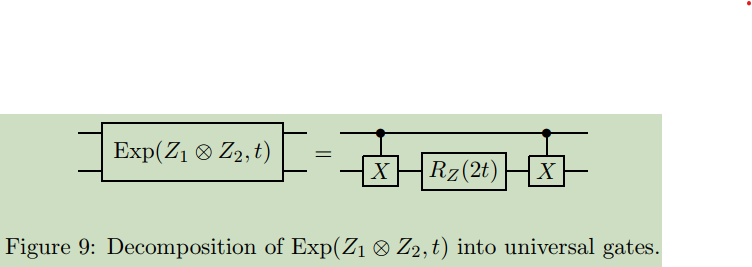
\includegraphics[width=0.75\linewidth]{Images/grange23-f9.png}
\end{figure}
On the one hand, (34) is the application of the gate $=\left(\begin{array}{cc}R_{Z}(2 t) & 0 \\ 0 & R_{Z}(-2 t)\end{array}\right)$ to this system. Indeed,

\begin{equation}
\begin{aligned}
\cos (t) I-i \sin (t) Z_{1} \otimes Z_{2} & =\cos (t)\left(\begin{array}{llll}
1 & 0 & 0 & 0 \\
0 & 1 & 0 & 0 \\
0 & 0 & 1 & 0 \\
0 & 0 & 0 & 1
\end{array}\right)-i \sin (t)\left(\begin{array}{cccc}
1 & 0 & 0 & 0 \\
0 & -1 & 0 & 0 \\
0 & 0 & -1 & 0 \\
0 & 0 & 0 & 1
\end{array}\right) \\
& =\left(\begin{array}{cccc}
e^{-i t} & 0 & 0 & 0 \\
0 & e^{i t} & 0 & 0 \\
0 & 0 & e^{i t} & 0 \\
0 & 0 & 0 & e^{-i t}
\end{array}\right) \\
& =\left(\begin{array}{ccc}
R_{Z}(2 t) & 0 & \\
0 & R_{Z}(-2 t)
\end{array}\right) .
\end{aligned}
\end{equation}

On the other hand, the composition of gates $C X_{1,2} R_{Z, 2}(2 t) C X_{1,2}$ on this system amounts to
\begin{equation}
\begin{aligned}
C X_{1,2} R_{Z, 2}(2 t) C X_{1,2} & =\left(\begin{array}{cc}
I & 0 \\
0 & X
\end{array}\right)\left(\begin{array}{cc}
R_{Z}(2 t) & 0 \\
0 & R_{Z}(2 t)
\end{array}\right)\left(\begin{array}{ll}
I & 0 \\
0 & X
\end{array}\right) \\
& =\left(\begin{array}{cc}
R_{Z}(2 t) & 0 \\
0 & X R_{Z}(2 t) X
\end{array}\right) \\
& =\left(\begin{array}{cc}
R_{Z}(2 t) & 0 \\
0 & R_{Z}(-2 t)
\end{array}\right) .
\end{aligned}
\end{equation}
Thus, the proof results from replacing $t$ by appropriate values $h_{i i} \gamma$ for $i \in[n]$ and $h_{i j} \gamma$ for $i<j$.
\end{proof}

The decomposition in universal quantum gates of the term $\operatorname{Exp}\left(Z_{i} \otimes Z_{j}, t\right)$ for the specific case of QUBO (see Proposition 35) is mainly used in the literature. 

% 2024-05-20 经LAI整理,已经初步完成

\chapter{Qaoa-in-qaoa: Solving Large-scale Maxcut Problems on Small Quantum Machines}
"QAOA-in-QAOA: solving large-scale MaxCut problems on small quantum machines" \cite{zhou2023qaoa}

% 有待整理

\chapter{Monte Carlo Policy Gradient Method for Binary Optimization}
"Monte Carlo Policy Gradient Method for Binary Optimization"

In this paper, we consider the following binary optimization problem:
\begin{equation}
    \min _{x} \quad f(x), \quad \text { s.t. } \quad x \in \mathcal{B}_{n} \tag{1}
\end{equation}
where $\mathcal{B}_{n}=\{-1,1\}^{n}$ represents the binary set of dimension $n$ and $f$ can be any function defined on $\mathcal{B}_{n}$.

\section{2 Probabilistic Model for Binary Optimization}

\subsection{2.1 Parameterized Probabilistic Model}

The goal is to search for the set of (globally) optimal points $\mathcal{X}^{*}$ of (1) in the discrete space $\mathcal{B}_{n}$. A probabilistic approach is to consider an \textbf{indicator distribution}, i.e.,
\begin{equation}
    q^{*}(x)=\frac{1}{\left|\mathcal{X}^{*}\right|} \mathbb{1}_{\mathcal{X}^{*}}(x)= 
\begin{cases}\frac{1}{\left|\mathcal{X}^{*}\right|}, & x \in \mathcal{X}^{*}, \\ 0, & x \notin \mathcal{X}^{*}.
\end{cases}
\end{equation}
Here,
\begin{equation}
    \mathbb{1}_{\mathcal{X}}(x)= \begin{cases}1, & x \in \mathcal{X}^*, \\ 0, & x \notin \mathcal{X}^* .\end{cases}
\end{equation}
The distribution $q^{*}$ is the ideal distribution where only the optimal points have the uniform probability. If we sample according to $q^{*}$, then we will definitely get the optimal solution of (1). However, the optimal points set $\mathcal{X}^{*}$ is unknown. 

To approach $q^{*}$, we introduce the following family of \textbf{Gibbs distributions} with parameter $\lambda > 0$:
\begin{equation}
    q_{\lambda}(x)=\frac{1}{Z_{\lambda}} \exp \left(-\frac{f(x)}{\lambda}\right), \quad x \in \mathcal{B}_{n}, \tag{3}
\end{equation}
where $Z_{\lambda}=\sum_{x \in \mathcal{B}_{n}} \exp \left(-\frac{f(x)}{\lambda}\right)$ is the normalization factor. Given the (globally) optimal value $f^{*}$ of (1), for any $x \in \mathcal{B}_{n}$, we notice that
\begin{align}
q_{\lambda}(x) & =\frac{\exp \left(\frac{-f(x)}{\lambda}\right)}{\sum_{x \in \mathcal{B}_{n}} \exp \left(\frac{-f(x)}{\lambda}\right)} \\
& =\frac{\exp \left(\frac{f^{*}-f(x)}{\lambda}\right)}{\sum_{x \in \mathcal{B}_{n}} \exp \left(\frac{f^{*}-f(x)}{\lambda}\right)} \\
&=\frac{\exp \left(\frac{f^{*}-f(x)}{\lambda}\right)}{\left|\mathcal{X}^{*}\right|+\sum_{x \in \mathcal{B}_{n} / \mathcal{X}^{*}} \exp \left(\frac{f^{*}-f(x)}{\lambda}\right)}  \tag{4}\\
& \rightarrow q^{*}(x)=\frac{1}{\left|\mathcal{X}^{*}\right|} \mathbb{1}_{\mathcal{X}^{*}}(x), \quad \text { as } \lambda \rightarrow 0.
\end{align}
Note that the term in denominator, namely, $\sum_{x \in \mathcal{B}_n / \mathcal{X}^*} \exp \left(\frac{f^*-f(x)}{\lambda}\right) \to 0$ as $\lambda \to 0$. Although $q^{*}$ is not computable in practice, the Gibbs distribution $q_{\lambda}$, which converges to $q^{*}$ pointwisely, provides a feasible alternative for searching optimal solutions. In summary, for all points $x \in\mathcal{B}_n$, 
one has
\begin{equation}
    q_\lambda(x) \to q^*(x)=\frac{1}{\left|\mathcal{X}^*\right|} \mathbf{1}_{\mathcal{X}^*}(x), \quad \text { as } \lambda \rightarrow 0.
\end{equation}
\begin{remark}
    We had encoded the information of objective function $f$ of (1) into the probabilistic models, both $q^{*}$ without parameters and $q_\lambda$ with parameters $\lambda$.
\end{remark}

Motivated by this observation, one can devise an algorithm to randomly sample from the Gibbs distribution and control the parameter $\lambda$ to approximate the global optimum. 
\begin{enumerate}
    \item However, since $q_{\lambda}(x)$ needs to compute the summation of $2^{n}$ terms in the denominator $Z_{\lambda}$, the complexity of direct sampling grows exponentially.
    \item Meanwhile, $q_{\lambda}$ is hard to sample when $f$ owns a rough landscape.
\end{enumerate}

Instead of direct sampling from the Gibbs distribution, we approximate it using a parameterized policy distribution that can be sampled efficiently. 

Consider the problem instance $\mathcal{P}$, that is, a instance of objective $f$. For the moment, $\lambda >0$ is a constant that was set in advance. The parameterized \textit{policy distribution} $p_{\theta}(x \mid \mathcal{P})$ is designed to have a similar but regular landscape to that of $q_{\lambda}$ to enable efficient sampling. For notational convenience, we write
\begin{equation}
    p_{\theta}(x)=p_{\theta}(x \mid \mathcal{P}).
\end{equation}
(We shall give the concrete way to construct $p_{\theta}$ in next section.) To measure the distance between $p_{\theta}$ and $q_{\lambda}$, we introduce the \textbf{KL divergence} defined as follows:
\begin{equation}
    \mathrm{KL}\left(p_{\theta} \| q_{\lambda}\right)=\sum_{x \in \mathcal{B}_{n}} p_{\theta}(x) \log \frac{p_{\theta}(x)}{q_{\lambda}(x)}.
\end{equation}
In order to reduce the discrepancy between the policy distribution $p_{\theta}$ and the Gibbs distribution $q_{\lambda}$, we minimize this KL divergence with respect to the variable $\theta$. For the Gibbs distribution $q_\lambda$ in (3), we notice that
\begin{align}
\min _{\theta} \quad \mathrm{KL}\left(p_{\theta} \| q_{\lambda}\right) 
& =\sum_{x \in \mathcal{B}_{n}} p_{\theta}(x) \left( \log p_{\theta}(x) - \log q_{\lambda}(x) \right) \\
& =\sum_{x \in \mathcal{B}_{n}} p_{\theta}(x) \left( \log  p_{\theta}(x) - \log \left[ \frac{1}{Z_\lambda} \exp \left(-\frac{f(x)}{\lambda}\right) \right]\right)  \\
& =\sum_{x \in \mathcal{B}_{n}} p_{\theta}(x) \left( \log  p_{\theta}(x) - \log \frac{1}{Z_\lambda} + \frac{f(x)}{\lambda}\right) \\
& =\frac{1}{\lambda} \sum_{x \in \mathcal{B}_{n}} p_{\theta}(x) f(x)+\sum_{x \in \mathcal{B}_{n}} p_{\theta}(x) \log p_{\theta}(x)+\log Z_{\lambda} \\
& =\frac{1}{\lambda}\left(\mathbb{E}_{p_{\theta}}[f(x)]+\lambda \mathbb{E}_{p_{\theta}}\left[\log p_{\theta}(x)\right]\right)+\log Z_{\lambda} ,\tag{5}
\end{align} 
where we write 
\begin{equation}
    \mathbb{E}_{p_\theta}[f(x)] = \sum_{x \in \mathcal{B}_n} p_\theta(x) f(x)
\end{equation}
and
\begin{equation}
    \mathbb{E}_{p_\theta}\left[\log p_\theta(x)\right] = \sum_{x \in \mathcal{B}_n} p_\theta(x) \log p_\theta(x).
\end{equation}
Since $Z_{\lambda}$ is a constant, (5) is equivalent to the following problem:
\begin{equation}
    \min _{\theta} \quad L_{\lambda}(\theta)=\underbrace{\mathbb{E}_{p_{\theta}}[f(x)]}_{L(\theta)}+\lambda \underbrace{\mathbb{E}_{p_{\theta}}\left[\log p_{\theta}(x)\right]}_{H(\theta)} \tag{6}
\end{equation}
While minimizing (6) is to find an approximation of Gibbs distribution $q_{\lambda}$, one can explain (6) from the perspective of optimization. 

In (6), the first term $L(\theta)$ is the expected loss of $f(x)$ with $x \sim p_{\theta}$ and the second term $H(\theta)$ is the \textit{entropy regularization} of $p_{\theta}$. 
\begin{itemize}
    \item Minimizing the first term $L(\theta)$ yields the optimal value $f^{*}$ and $p_{\theta}\left(x \in \mathcal{X}^{*}\right)=1$. However, it leads to hardship on sampling as $p_{\theta}$ is rough. By adding the entropy regularization, we encourage exploration and promote the diversity of samples.
    \item On the other hand, the\textit{ regularization parameter} $\lambda$, which is also called \textit{annealing temperature}, progressively decreases from an initial positive value to zero as in the classical simulated annealing, and the global optimum are finally obtained after a sufficiently long time.
\end{itemize}

\subsection{2.2 Parameterization of Sampling Policy Distribution $p_{\theta}$}

As we discuss above, we can use probabilistic methods to solve binary optimization problems. 

The sampling policy can be parameterized by a neural network with $\mathcal{P}$ containing features of the problem, that is,
\begin{equation}
    p_{\theta}(x \mid \mathcal{P}) \propto e^{\phi_{\theta}(x, \mathcal{P})} \tag{7}
\end{equation}
where $\phi$ represents a neural network with input $x$ and problem instance $\mathcal{P}$. 

It is unrealistic to generate a normalized distribution over $2^{n}$ points in $\mathcal{B}_{n}$. The unnormalized policy (7) can be sampled through the Metropolis algorithm. The neural network can be designed to reduce the computational complexity in the sampling process. % 但是实验也没有用到neural network啊

One natural idea is to consider the distribution on each single variable (that is, each $x_{i} \in \{-1,+1\}$ in binary string $x=x_{1}x_{2}\dots x_{n}$ ) and assume independence, which is called the \textbf{mean field (MF) approximation} in statistical physics. 

The MF methods provide tractable approximations for the high dimensional computation in probabilistic models. By neglecting certain dependencies between random variables, we simplify the parameterized distribution $p_{\theta}$ with the independent assumption for each component of $x$. As for binary optimization problems $\mathcal{P}$ in (1), the parameterized probability follows the \textit{multivariate Bernoulli distribution}:
\begin{equation}
    p_{\theta}(x)=\prod_{i=1}^{n} \mu_{i}^{\left(1+x_{i}\right) / 2}\left(1-\mu_{i}\right)^{\left(1-x_{i}\right) / 2}, \quad \mu_{i}=\operatorname{sigmoid}(x_i)=\frac{1}{1+e^{-\theta_{i}}}, \tag{8}
\end{equation}
where $\theta_{i}, i=1, \ldots, n$ are parameters. Under the mean field approximation, $x_{1}, x_{2}, \ldots, x_{n}$ are viewed independent and $\mu_{i}$ is the probability that the $i$-th variable $x_{i}$ takes value "+1". Note that $\left(1+x_{i}\right)/2=1$ and $\left(1-x_{i}\right)/2=0$ for $x_i = +1$; on the other hand, $\left(1+x_{i}\right)/2=0$ and $\left(1-x_{i}\right)/2=1$ for $x_i = -1$.

The MF approximation provides an efficient way to encode binary optimization problems and greatly reduces the complexity of the model from $2^{n}$ to $n$. Besides, the distribution under MF approximation is beneficial for the Markov chain Monte Carlo sampling. %  encode binary optimization problems, 这里唯一编码了问题的可行解,即binary特征,而和f无关。

\subsection{2.3 Prototype Algorithm}

In the above discussion, we have already constructed the loss function $L_{\lambda}(\theta)$ and a mean field sampling policy $p_{\theta}(x)$. Sometimes, we often only say "policy", or "sampling policy" for the short of "sampling policy distribution $p_{\theta}$".

To train the policy, the gradient formulation is derived explicitly in following Lemma 1. Then, we purpose the brief algorithm framework. The sampled solutions help to compute the policy gradient and improve the sampling policy. The policy is optimized by the stochastic policy gradient, which guides us to sample those points with lower function values. Thus, the binary optimization problems are solved by stochastic sampling based on a neural network policy. % neural network policy 怎么又出现了nn?有没有用到。

\begin{lemma}[Lemma 1]
    Suppose for any $x \in \mathcal{B}_{n}$, the policy $p_{\theta}(x)$ is differentiable with respect to $\theta$. For any constant $c \in \mathbb{R}$, the gradient of the loss function (6) is given by
\begin{equation}
    \nabla_{\theta} L_{\lambda}(\theta)=\mathbb{E}_{p_{\theta}}\left[\left(f(x)+\lambda \log p_{\theta}(x)-c\right) \nabla_{\theta} \log p_{\theta}(x)\right]. \tag{9}
\end{equation}
This gradient is called the policy gradient.
\end{lemma}
\begin{proof}
    By exchanging the order of differentiation ($\nabla$ operations) and summation, we note that
\begin{align}
\mathbb{E}_{p_{\theta}}\left[\nabla_{\theta} \log p_{\theta}(x)\right]
&=\mathbb{E}_{p_{\theta}}\left[ \frac{1}{p_{\theta}(x)}\nabla_{\theta} p_{\theta}(x)\right] \\
&=\sum_{x \in \mathcal{B}_{n}} p_{\theta}(x) \cdot \frac{1}{p_{\theta}(x)}\nabla_{\theta} p_{\theta}(x)\\
&=\sum_{x \in \mathcal{B}_{n}} \nabla_{\theta} p_{\theta}(x) \\
&=\nabla_{\theta} \sum_{x \in \mathcal{B}_{n}} p_{\theta}(x) \\
&=\nabla_{\theta} 1=0 \tag{10}
\end{align}
as $\sum_{x \in \mathcal{B}_{n}} p_{\theta}(x)=1$ is a constant. The gradient of the loss function (6) 
\begin{align}
    L_{\lambda}(\theta) &= \sum_{x \in \mathcal{B}_n} p_\theta(x) f(x)+ \lambda \sum_{x \in \mathcal{B}_n} p_\theta(x) \log p_\theta(x) \\
    & = \sum_{x \in \mathcal{B}_n} p_\theta(x)\left(f(x)+\lambda \log p_\theta(x)\right).
\end{align}
is derived by
\begin{equation}
\begin{aligned}
\nabla_{\theta} L_{\lambda}(\theta) & =\nabla_{\theta} \sum_{x \in \mathcal{B}_{n}} p_{\theta}(x)\left(f(x)+\lambda \log p_{\theta}(x)\right) \\
& =\lambda \sum_{x \in \mathcal{B}_{n}} p_{\theta}(x) \nabla_{\theta} \log p_{\theta}(x)+\sum_{x \in \mathcal{B}_{n}}\left(f(x)+\lambda \log p_{\theta}(x)\right) \nabla p_{\theta}(x) \\
& \stackrel{(i)}{=} \lambda \sum_{x \in \mathcal{B}_{n}} \nabla_{\theta} p_{\theta}(x)+\sum_{x \in \mathcal{B}}\left(f(x)+\lambda \log p_{\theta}(x)\right) p_{\theta}(x) \nabla_{\theta} \log p_{\theta}(x) \\
& \stackrel{(i i)}{=} \sum_{x \in \mathcal{B}} p_{\theta}(x) \left(f(x)+\lambda \log p_{\theta}(x)\right)  \nabla_{\theta} \log p_{\theta}(x) \\
& =\mathbb{E}_{p_{\theta}}\left[\left(f(x)+\lambda \log p_{\theta}(x)\right) \nabla_{\theta} \log p_{\theta}(x)\right]
\end{aligned}
\end{equation}

where ( $i$ ) uses the substitution 
\begin{equation}
    \nabla_{\theta} p_{\theta}(x)=p_{\theta}(x) \cdot \nabla_{\theta} \log p_{\theta}(x)
\end{equation}
and (ii) is due to (10). For any given $c$ irrelevant to $x,(10)$ yields that $\mathbb{E}_{p_{\theta}}\left[c \nabla_{\theta} \log p_{\theta}(x)\right]=0$. This completes the proof.
\end{proof}

Especially, we take % c 是依赖于theta的值,可以这么取常数c吗?
\begin{equation}
    c=\mathbb{E}_{p_{\theta}}[f(x)]
\end{equation}
and denote 
\begin{equation}
    A_{\lambda}(x ; \theta)=f(x)+\lambda \log p_{\theta}(x)- \mathbb{E}_{p_{\theta}}[f(x)].
\end{equation}
In this case, the policy gradient is 
\begin{equation}
    \nabla_\theta L_\lambda(\theta)=\mathbb{E}_{p_\theta}\left[ A_{\lambda}(x ; \theta) \cdot \nabla_\theta \log p_\theta(x)\right].
\end{equation}
We call the function $A_{\lambda}(x ; \theta)$ as the "\textbf{advantage function}" analogous to the one in reinforcement learning [40]. It has been shown that such technique can reduce the variance in our training and make it easier to sample points with lower cost. 

Hence, the stochastic gradient is computed by
\begin{equation}
\begin{aligned}
A_{\lambda}(x ; \theta, S) & =f(x)+\lambda \log p_{\theta}(x)-\sum_{x \in S} f(x), \\
\bar{g}(\theta, S) & =\sum_{x \in S} A_{\lambda}(x ; \theta, S) \nabla_{\theta} \log p_{\theta}(x).
\end{aligned}
\end{equation}
where $S$ is a sample set from the distribution $p_{\theta}(x)$.

Finally, we propose a prototype algorithm for solving binary optimization problems as follows:

\begin{enumerate}
    \item At the beginning of each iteration, the probabilistic model provides a distribution $p_{\theta}(\cdot \mid \mathcal{P})$, indicating where the good solution potentially lies.
    \item A set of points $S$ are sampled from $p_{\theta}(\cdot \mid \mathcal{P})$.
    \item The policy gradient is computed in order to update the probabilistic model, providing an improved distribution for the next iteration.
    \item The parameter $\theta$ in the probabilistic model is updated as follows
  \begin{equation}
    \theta^{t+1}=\theta^{t}-\eta^{t} \bar{g}\left(\theta^{t}, S^{t}\right)
\end{equation}
  where $\eta^{t}$ and $S^{t}$ are the step size and the sample set at the $t$-th iteration.
\end{enumerate}

Algorithm 1 gives the pseudo-code of the prototype algorithm. 
\begin{figure}
    \centering
    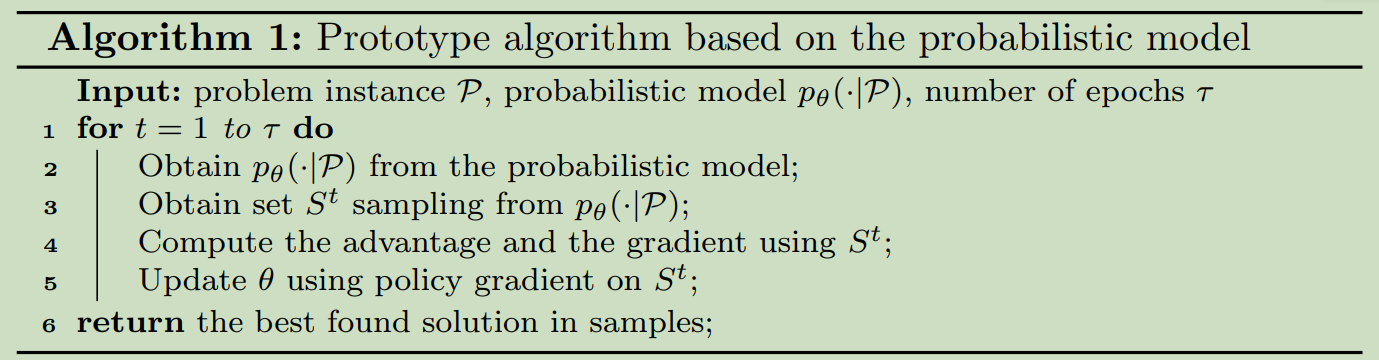
\includegraphics[width=1\linewidth]{Images/MCPG_ALG_1.png}
\end{figure}
The prototype algorithm is efficient in obtaining better solutions compared to most naive heuristic methods, since similar frameworks are commonly used in machine learning. However, it also faces several critical challenges. 
\begin{itemize}
    \item It is difficult to determine whether a good solution has been achieved.
    \item Moreover, keeping the diversity of samples remains challenges at the later iterations. On the other hand, due to the NP-hard nature of the problem (1), there are many local minimum in solving problem (6), making it challenging for policy gradient methods to find global minima. This difficulty is prevalent in most reinforcement learning scenarios.
\end{itemize}

\section{3 A Monte Carlo Policy Gradient Method} %至此,我们没有解释具体如何根据p_theta采样得到S,本节的3.1,3.2的算法的目的就是详述采样的一个好办法。可以直接跳到3.3节看整体。

\begin{figure}
    \centering
    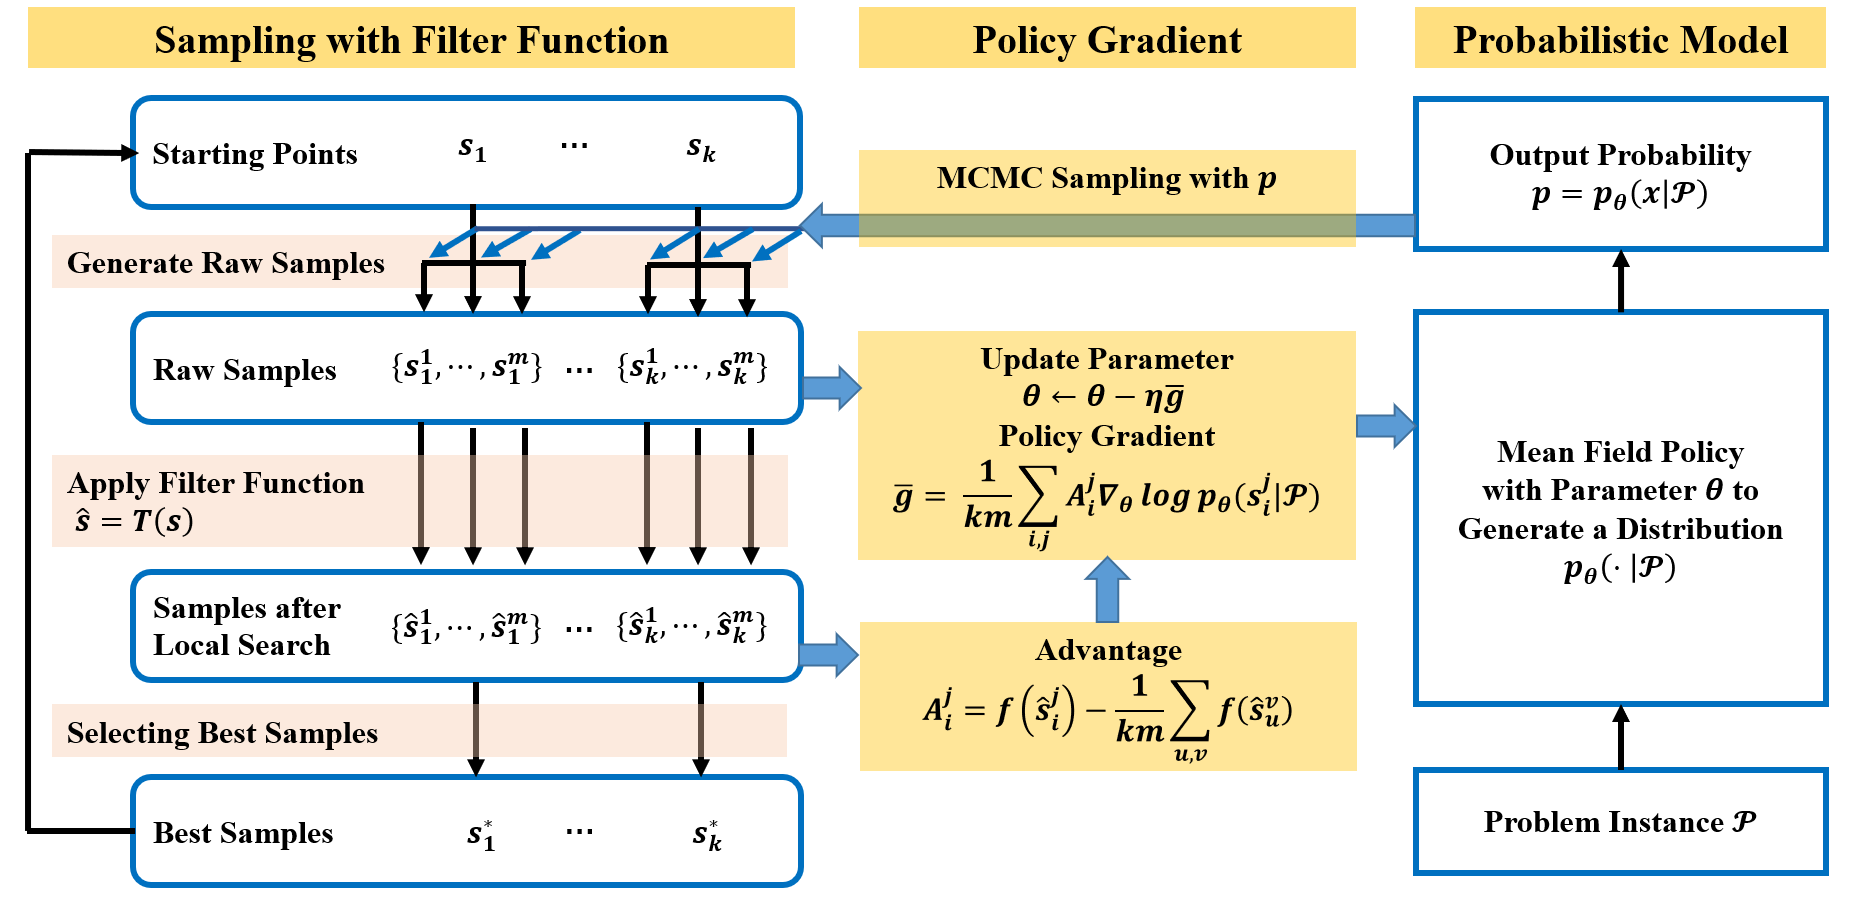
\includegraphics[width=1\linewidth]{Images/MCPG_pipeline.png}
    \caption{Enter Caption}
    \label{fig:enter-label}
\end{figure}

\begin{figure}
    \centering
    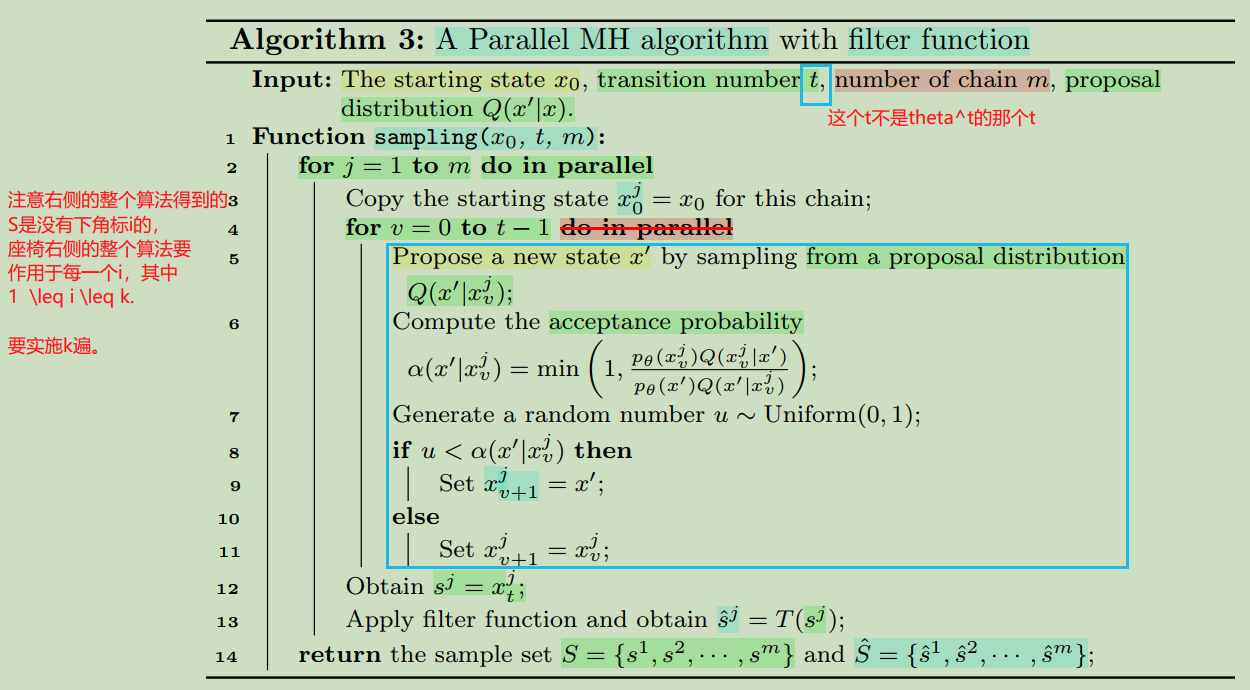
\includegraphics[width=1\linewidth]{Images/MCPG_ALG_3.png}
\end{figure}

\begin{figure}
    \centering
    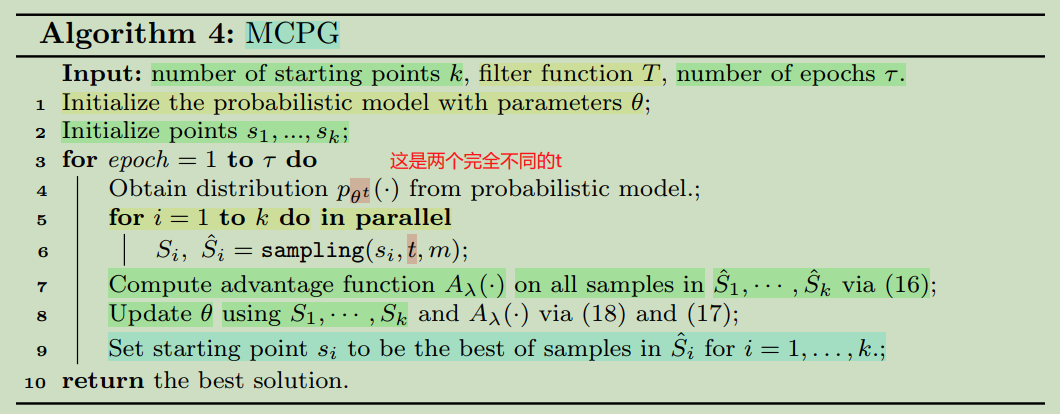
\includegraphics[width=1\linewidth]{Images/MCPG-ALG-4.png}
\end{figure}



\chapter{Estimating the gradient and higher-order derivatives on quantum hardware}
\href{https://journals.aps.org/pra/abstract/10.1103/PhysRevA.103.012405}{Phys. Rev. A 103, 012405 (2021) - Estimating the gradient and higher-order derivatives on quantum hardware (aps.org)}  \cite{mari2021estimating}

\section{II. SETTING: Variational Optimization of Quantum Circuits}

A variational quantum circuit acting on $n$ qubits is a sequence of gates depending on a set of classical parameters $\boldsymbol{\theta}=\left(\theta_1, \theta_2, \ldots, \theta_m\right)$ and producing a family of unitary operations $U(\theta)$. 

A typical structure of many variational circuits which can be executed by near-term quantum computers is
\begin{equation}
    U(\boldsymbol{\theta})=V_m U_m\left(\theta_m\right) \cdots V_2 U_2(\theta) V_1 U_1\left(\theta_1\right),
\end{equation}
where $V_j$ are constant arbitrary circuits, while $U_j\left(\theta_j\right)$ are \textbf{rotation-like gates}, i.e., characterized by a Hermitian\footnote{$U_j\left(\theta_j\right)^{\dagger} U_j\left(\theta_j\right)=e^{(i / 2) H_j \theta_j} e^{-(i / 2) H_j \theta_j}=e^0=\mathbf{1}$.} generator $H_j$ such that $H_j^2=\textbf{1}$ (i.e., involutory matrix) and so
\begin{equation}
    U_j\left(\theta_j\right)=e^{-(i / 2) H_j \theta_j}=\cos \left(\theta_j / 2\right) \textbf{1}-i \sin \left(\theta_j / 2\right) H_j .
\end{equation}
Note the last equality holds only if $H_j$ is involutory. (For proof see Appendix \ref{app:a0})

Typically, the circuit is applied to a fixed reference state $|0\rangle$ and the expectation value of a Hermitian observable $M$\footnote{$M$ must be Hermitian.} is measured:
\begin{equation}\label{eq:cost}
    f(\boldsymbol{\theta})=\left\langle 0\left|U(\boldsymbol{\theta})^{\dagger} M U(\boldsymbol{\theta})\right| 0\right\rangle .
\end{equation}
The expectation value given in Eq. (\ref{eq:cost}) is usually optimized with respect to the parameters $\boldsymbol{\theta}$. 

In this work we are interested in evaluating derivatives of an arbitrary order $d$, which we can cast as a tensor with $d$ indices $j_1, j_2, \ldots, j_d$ whose elements are the real quantities
\begin{equation}\label{eq:deribatives}
    g_{j_1, j_2, \ldots, j_d}(\boldsymbol{\theta})=\frac{\partial^d f(\boldsymbol{\theta})}{\partial \theta_{j_1} \partial \theta_{j_2} \cdots \partial \theta_{j_d}},
\end{equation}
where the gradient and the Hessian correspond to the particular cases with $d=1$ and $d=2$, respectively. 

\section{III. PARAMETER-SHIFT RULES}

\subsection{A. First-order Derivatives: The Gradient}

In what follows, we will fix the index $j$, and only consider univariate of $\theta_j$.

\begin{lemma}
    The \textbf{unitary conjugation} of an arbitrary operator $\hat{K}$ by $U_j\left(\theta_j\right)$, namely, $U_j\left(\theta_j\right)^{\dagger} \hat{K} U_j\left(\theta_j\right)$, can always be reduced to the sum of three terms
\begin{equation}
    \hat{K}\left(\theta_j\right):=U_j\left(\theta_j\right)^{\dagger} \hat{K} U_j\left(\theta_j\right)=\hat{A}+\hat{B} \cos \left(\theta_j\right)+\hat{C} \sin \left(\theta_j\right),
\end{equation}
where $\hat{A}, \hat{B}$, and $\hat{C}$ are operators independent of $\theta_j$ and involving only $\hat{K}$ and $\hat{H}_j$.
\end{lemma}

\begin{proof}
 The conjugate transpose of $U_j(\theta_j)$ is
\begin{equation}
    U_j(\theta_j)^{\dagger} = \cos \left(\theta_j / 2\right) \textbf{1} + i \sin \left(\theta_j / 2\right) H_j.
\end{equation}
So,
\begin{equation}
    \hat{K}(\theta_j) = \left( \cos \left(\theta_j / 2\right) \textbf{1} + i \sin \left(\theta_j / 2\right) H_j \right) \hat{K} \left( \cos \left(\theta_j / 2\right) \textbf{1} - i \sin \left(\theta_j / 2\right) H_j \right).
\end{equation}
Expanding this product yields
\begin{equation}
    \hat{K}(\theta_j) = \cos^2 \left(\theta_j / 2\right) \hat{K} - i \cos \left(\theta_j / 2\right) \sin \left(\theta_j / 2\right) \hat{K} H_j + i \cos \left(\theta_j / 2\right) \sin \left(\theta_j / 2\right) H_j \hat{K} + \sin^2 \left(\theta_j / 2\right) H_j \hat{K} H_j.
\end{equation}
Using the trigonometric identities:
\begin{equation}
    \cos^2 \left(\theta_j / 2\right) = \frac{1 + \cos(\theta_j)}{2}, \quad \sin^2 \left(\theta_j / 2\right) = \frac{1 - \cos(\theta_j)}{2}, \quad \cos \left(\theta_j / 2\right) \sin \left(\theta_j / 2\right) = \frac{\sin(\theta_j)}{2},
\end{equation}
we have
\begin{equation}
    \hat{K}(\theta_j) = \left( \frac{1 + \cos(\theta_j)}{2} \right) \hat{K} - i \left( \frac{\sin(\theta_j)}{2} \right) \hat{K} H_j + i \left( \frac{\sin(\theta_j)}{2} \right) H_j \hat{K} + \left( \frac{1 - \cos(\theta_j)}{2} \right) H_j \hat{K} H_j.
\end{equation}
Grouping the terms, we obtain:
\begin{equation}
    \hat{K}(\theta_j) = \frac{1}{2} \hat{K} + \frac{1}{2} \cos(\theta_j) \hat{K} - \frac{i}{2} \sin(\theta_j) \hat{K} H_j + \frac{i}{2} \sin(\theta_j) H_j \hat{K} + \frac{1}{2} H_j \hat{K} H_j - \frac{1}{2} \cos(\theta_j) H_j \hat{K} H_j
\end{equation}
Defining $\hat{A}$, $\hat{B}$, and $\hat{C}$ as:
\begin{equation}
    \hat{A} = \frac{1}{2} (\hat{K} + H_j \hat{K} H_j), \quad \hat{B} = \frac{1}{2} (\hat{K} - H_j \hat{K} H_j), \quad \hat{C} = \frac{i}{2} (H_j \hat{K} - \hat{K} H_j)
\end{equation}
Finally, we get:
\begin{equation}
    \hat{K}(\theta_j) = \hat{A} + \hat{B} \cos(\theta_j) + \hat{C} \sin(\theta_j).
\end{equation}
Thus, the unitary conjugation of an arbitrary operator $\hat{K}$ by $U_j(\theta_j)$ can always be reduced to the sum of three terms involving operators $\hat{A}$, $\hat{B}$, and $\hat{C}$ that are independent of $\theta_j$.
\end{proof}

Moreover, from the standard trigonometric addition and subtraction identities, we can deduce the following lemma.

\begin{lemma}
\begin{align}
& \frac{d \cos (x)}{d x}=\frac{\cos (x+s)-\cos (x-s)}{2 \sin (s)}, \\
& \frac{d \sin (x)}{d x}=\frac{\sin (x+s)-\sin (x-s)}{2 \sin (s)},
\end{align}
which are valid for any $s \neq k \pi, k \in \mathbb{Z}$.
\end{lemma}

\begin{proof}
    We only give the poofs for the cosine identity. Recall the addition and subtraction formulas for cosine:
\begin{align}
& \cos (x+s)=\cos (x) \cos (s)-\sin (x) \sin (s), \\
& \cos (x-s)=\cos (x) \cos (s)+\sin (x) \sin (s).
\end{align}
Hence,
\begin{equation}
    \frac{\cos (x+s)-\cos (x-s)}{2 \sin (s)}=\frac{-2 \sin (x) \sin (s)}{2 \sin (s)}=-\sin (x).
\end{equation}
\end{proof}

Now, differentiate $\hat{K}\left(\theta_j\right)$ with respect to $\theta_j$:
\begin{align}
\frac{\partial \hat{K}\left(\theta_j\right)}{\partial \theta_j}
&=\hat{B}\frac{\partial \cos \left(\theta_j\right)}{\partial \theta_j} +\hat{C}\frac{\partial \sin \left(\theta_j\right)}{\partial \theta_j} \\
&=\hat{B}\left(\frac{\cos \left(\theta_j+s\right)-\cos \left(\theta_j-s\right)}{2 \sin (s)}\right)+\hat{C}\left(\frac{\sin \left(\theta_j+s\right)-\sin \left(\theta_j-s\right)}{2 \sin (s)}\right).
\end{align}
On the other hand, recognize that $\hat{K}\left(\theta_j \pm s\right)$ can be written as
\begin{align}
\hat{K}\left(\theta_j+s\right) & =\hat{A}+\hat{B} \cos \left(\theta_j+s\right)+\hat{C} \sin \left(\theta_j+s\right),\\
\hat{K}\left(\theta_j-s\right) & =\hat{A}+\hat{B} \cos \left(\theta_j-s\right)+\hat{C} \sin \left(\theta_j-s\right).
\end{align}
Thus, we get the next lemma.

\begin{lemma}
\begin{equation}
    \frac{\partial \hat{K}\left(\theta_j\right)}{\partial \theta_j}=\frac{\hat{K}\left(\theta_j+s\right)-\hat{K}\left(\theta_j-s\right)}{2 \sin (s)}.
\end{equation}
\end{lemma}

Recall that
\begin{equation}
    U(\boldsymbol{\theta})=V_m U_m\left(\theta_m\right) \cdots V_j U_j\left(\theta_j\right) \cdots V_1 U_1\left(\theta_1\right),
\end{equation}
and
\begin{equation}
    U(\boldsymbol{\theta})^{\dagger}=U_1\left(\theta_1\right)^{\dagger} V_1^{\dagger} \cdots U_j\left(\theta_j\right)^{\dagger} V_j^{\dagger} \cdots U_m\left(\theta_m\right)^{\dagger} V_m{ }^{\dagger}.
\end{equation}
Then, 
\begin{align}
f(\boldsymbol{\theta}) & =\left\langle 0\left|U(\boldsymbol{\theta})^{\dagger} M U(\boldsymbol{\theta})\right| 0\right\rangle .\\
& =\underbrace{\langle 0| U_1\left(\theta_1\right)^{\dagger} V_1^{\dagger} \cdots}_{\langle\psi|:=} 
U_j\left(\theta_j\right)^{\dagger} 
\underbrace{V_j^{\dagger} \cdots U_m\left(\theta_m\right)^{\dagger} V_m{ }^{\dagger}  M V_m U_m\left(\theta_m\right) \cdots V_j}_{\hat{K}:=}   
U_j\left(\theta_j\right) \underbrace{\cdots V_1 U_1\left(\theta_1\right)| 0 \rangle }_{|\psi\rangle :=}.\\
&=\left\langle\psi\left|U_j\left(\theta_j\right)^{\dagger} \hat{K} U_j\left(\theta_j\right)\right| \psi\right\rangle \\
&=\left\langle\psi\left|  \hat{K}\left(\theta_j\right) \right| \psi\right\rangle \\
&\equiv f(\underbrace{\theta_1, \cdots}_{\text {Seem as fixed}}, \theta_j, \underbrace{\cdots, \theta_m}_{\text {Seem as fixed}}).
\end{align}
Hence, we have 
\begin{align}
\frac{\partial f(\boldsymbol{\theta})}{\partial \theta_j} 
& =\frac{\partial}{\partial \theta_j}   f(\underbrace{\theta_1, \cdots}_{\text {Seem as fixed}}, \theta_j, \underbrace{\cdots, \theta_m}_{\text {Seem as fixed}}) \\
& =\frac{\partial}{\partial \theta_j}\left(\left\langle\psi\left|\hat{K}\left(\theta_j\right)\right| \psi\right\rangle\right) \\ 
& =\left\langle\psi\left|\frac{\partial}{\partial j} \hat{K}\left(\theta_j\right)\right| \psi\right\rangle \\
& =\left[\left\langle\psi\left|\hat{K}\left(\theta_j+s\right)\right| \psi\right\rangle-\left\langle\psi\left|\hat{K}\left(\theta_j-s\right)\right| \psi\right\rangle\right] \cdot \frac{1}{2 \sin (s)} \\
& =\frac{f\left(\boldsymbol{\theta}+s \mathbf{e}_j\right)-f\left(\boldsymbol{\theta}-s \mathbf{e}_j\right)}{2 \sin (s)},
\end{align}
where $\mathbf{e}_j$ is the unit vector along the $\theta_j$ axis.

\begin{theorem}
    Finally, to evaluate the $j$ th component of the gradient. The result is a family of parameter-shift rules
\begin{equation}\label{eq:gradient-PSR}
    g_j(\boldsymbol{\theta})=\frac{f\left(\boldsymbol{\theta}+s \mathbf{e}_j\right)-f\left(\boldsymbol{\theta}-s \mathbf{e}_j\right)}{2 \sin (s)}, \quad \forall j \in \{1,\dots,m\},
\end{equation}
which are valid for any $s \neq k \pi, k \in \mathbb{Z}$.
\end{theorem}

Notice that
\begin{enumerate}
    \item In the limit $s \rightarrow 0, \sin (s)$ can be approximated by $s$ and we recover the central-difference approximation for the first derivative.
    \item It is important to remark that the formula in Eq. (\ref{eq:gradient-PSR}) is \textit{exact} for \textit{any choice} of $s \neq k \pi, k \in \mathbb{Z}$.
\end{enumerate}

\subsection{B. Second-order Derivatives: The Hessian}

A useful property of Eq. (\ref{eq:gradient-PSR}) is that it can be iterated to get higher-order derivatives. 

\begin{theorem}
    Applying the same rule twice, i.e., applying (\ref{eq:gradient-PSR}) to itself, we get a similar formula for the Hessian,
\begin{align}
g_{j_1, j_2}(\boldsymbol{\theta})= & {\left[f\left(\boldsymbol{\theta}+s_1 \mathbf{e}_{j_1}+s_2 \mathbf{e}_{j_2}\right)-f\left(\boldsymbol{\theta}-s_1 \mathbf{e}_{j_1}+s_2 \mathbf{e}_{j_2}\right)\right.} \\
& \left.-f\left(\boldsymbol{\theta}+s_1 \mathbf{e}_{j_1}-s_2 \mathbf{e}_{j_2}\right)+f\left(\boldsymbol{\theta}-s_1 \mathbf{e}_{j_1}-s_2 \mathbf{e}_{j_2}\right)\right] \\
& \times \left[4 \sin \left(s_1\right) \sin \left(s_2\right)\right]^{-1}, \quad \forall j_1,j_2 \in \{1,\dots,m\},
\end{align}
which, for $s_1=s_2=s$, simplifies to
\begin{align}\label{eq:hessiamPSR}
g_{j_1, j_2}(\boldsymbol{\theta})=[ & f\left(\boldsymbol{\theta}+s\left(\mathbf{e}_{j_1}+\mathbf{e}_{j_2}\right)\right)-f\left(\boldsymbol{\theta}+s\left(-\mathbf{e}_{j_1}+\mathbf{e}_{j_2}\right)\right) \\
& \left.-f\left(\boldsymbol{\theta}+s\left(\mathbf{e}_{j_1}-\mathbf{e}_{j_2}\right)\right)+f\left(\boldsymbol{\theta}-s\left(\mathbf{e}_{j_1}+\mathbf{e}_{j_2}\right)\right)\right] \\
& \times  [2 \sin (s)]^{-2} , \quad \forall j_1,j_2 \in \{1,\dots,m\}.
\end{align}
\end{theorem}

Note that
\begin{enumerate}
    \item For $s \rightarrow 0$, we get the standard central difference formula for the Hessian.
    \item For each pair of $j_1,j_2$, we can choose different $s$ to evaluate $g_{j_1, j_2}(\boldsymbol{\theta})$. This is also true when we evaluate each component of gradient. In a word, the real number $s$ is independent to index $j$'s.
\end{enumerate}

\subsubsection{Diagonal of the Hessian}

Particular attention should be paid to the \textit{diagonal of the Hessian} (if $s_1=s_2=s$):
\begin{align}
g_{j, j}(\boldsymbol{\theta})=[ & f\left(\boldsymbol{\theta}+2s\mathbf{e}_{j}\right)
-2 f\left(\boldsymbol{\theta}\right) 
+ f\left(\boldsymbol{\theta}-2s\mathbf{e}_{j}\right)]
\times [2 \sin (s)]^{-2} , \quad \forall j \in \{1,\dots,m\},
\end{align}
since for each element, two shifts of $\pm s$ are applied to the same parameter $\theta_j$. 

In this case, two alternative choices for the value of $s$ are particularly relevant. Each of the two preceding formulas has alternative advantages.

\begin{enumerate}
    \item For the choice $s=\pi / 2$, we get
\begin{equation}
    g_{j, j}(\boldsymbol{\theta})=\left[f\left(\boldsymbol{\theta}+\pi \mathbf{e}_j\right)-f(\boldsymbol{\theta})\right] / 2,
\end{equation}
where we used that $f\left(\boldsymbol{\theta}+\pi \mathbf{e}_j\right)=f\left(\boldsymbol{\theta}-\pi \mathbf{e}_j\right)$.\footnote{Recall that $f\left(\boldsymbol{\theta}+\pi \mathbf{e}_j\right)=\langle\psi| \hat{K}(\theta_j+\pi)|\psi\rangle$ and $f\left(\boldsymbol{\theta}-\pi \mathbf{e}_j\right)=\langle\psi| \hat{K}(\theta_j-\pi)|\psi\rangle$. Indeed, 
\begin{align}
& \hat{K}\left(\theta_j+\pi\right)=\hat{A}+\hat{B} \cos \left(\theta_j+\pi\right)+\hat{C} \sin \left(\theta_j+\pi\right) \\
= & \hat{K}\left(\theta_j-\pi\right)=\hat{A}+\hat{B} \cos \left(\theta_j-\pi\right)+\hat{C} \sin \left(\theta_j-\pi\right)
\end{align}
since $\sin (\alpha \pm \pi)=-\sin (\alpha),\cos (\alpha \pm \pi)=-\cos (\alpha) .$} It involves only two expectation values and so it is more direct than next one.
    \item Instead, for $s=\pi / 4$, we obtain
\begin{equation}\label{eq:secondchose}
    g_{j, j}(\boldsymbol{\theta})=\left[f\left(\boldsymbol{\theta}+\mathbf{e}_j \pi / 2\right)-2 f(\boldsymbol{\theta})+f\left(\boldsymbol{\theta}-\mathbf{e}_j \pi / 2\right)\right] / 2 .
\end{equation}
\begin{enumerate}
    \item It involves are only $\pm \pi / 2$ type shifts. Assume that. This implies that \textit{all} the elements of the \textit{full} Hessian matrix can be evaluated using only the same type of $\pm \pi / 2$ shifts\footnote{Here, we assume that we choose $s=\pi / 2$ for all the other elements of Hessian.} and this fact could be an experimentally relevant simplification\footnote{Perhaps it's a matter of physical implementation.}.
    \item \textbf{(Interesting!)} Moreover, in the typical scenario (e.g., we use Newton method) in which one has already evaluated the gradient using the $m$ pairs of shifts $f\left(\theta \pm \pi / 2 \mathbf{e}_j\right)$ (i.e., we choose $s=\pi / 2$ in (\ref{eq:gradient-PSR})), then Eq. (\ref{eq:secondchose}) allows us to evaluate the diagonal of the Hessian with the extra cost of just a single expectation value, i.e., $f(\boldsymbol{\theta})$. This implies the cost of diagonal Newton method is little.
\end{enumerate}
\end{enumerate}

\subsection{C. Fubini-study Metric Tensor (quantum Natural Gradient)}

\todo{omitted}

\subsection{D. Arbitrary-order Derivatives}

The same iterative approach can be used to evaluate derivatives of arbitrary order. 

Now, we try to evaluate the derivatives of an arbitrary order $d$, i.e., the derivative tensor defined in Eq. (\ref{eq:deribatives}). In this case, for simplicity, we set the only choice $s=\pi / 2$ and we introduce the \textbf{multi-parameter shift vectors}:
\begin{equation}
    \mathbf{k}_{ \pm j_1, \pm j_2, \ldots, \pm j_d}=\frac{\pi}{2}\left( \pm \mathbf{e}_{j_1} \pm \mathbf{e}_{j_2} \pm \cdots \pm \mathbf{e}_{j_d}\right),
\end{equation}
where $j_1, j_2, \ldots, j_d \in \{1,\dots,m\}$. These vectors represent \textit{all the possible} shifts in parameter space that are generated by iterating the parameter-shift rule of Eq. (\ref{eq:gradient-PSR}) for $j \in$ $\left\{j_1, j_2, \ldots, j_d\right\}$. We explicitly introduce the set of all shifts which are related to a derivative of order $d$:
\begin{equation}
    S_{j_1, j_2, \ldots, j_d}=\left\{\mathbf{k}_{ \pm j_1, \pm j_2, \ldots, \pm j_d}, \forall \text { choices of signs }\right\},
\end{equation}
where $\left|S_{j_1, j_2, \ldots, j_d}\right|=2^d$. For example, for the Hessian formula given in Eq. (\ref{eq:hessiamPSR}) evaluated as $s=\pi / 2$, there are four possible shifts: $S_{j_1, j_2}=\left\{\mathbf{k}_{ \pm j_1, \pm j_2}\right\}$.

\begin{theorem}
    With this notation, the derivative tensor of order $d$ defined in Eq. (\ref{eq:deribatives}) can be expressed in terms of the generalized parameter-shift rule
\begin{equation}
    g_{j_1, j_2, \ldots, j_d}(\boldsymbol{\theta})=\frac{1}{2^d} \sum_{\mathbf{k} \in S_{j_1, j_2, \ldots j_d}} \mathcal{P}(\mathbf{k}) f(\boldsymbol{\theta}+\mathbf{k}),
\end{equation}
where $\mathcal{P}(\mathbf{k})$ is the parity of a shift vector, i.e., the \textit{parity of negative indices}. Specifically, $\mathcal{P}(\mathbf{k})$ is defined as $\mathcal{P}(\mathbf{k})=(-1)^{\sum_{i=1}^d \delta_{k_i,-1}}.$ Here, $\delta_{k_i,-1}$ is the Kronecker delta function, which is 1 if $k_i=-1$ and 0 otherwise.
\end{theorem}

\subsubsection{Complexity}

How many expectation values are necessary to evaluate the $d$-order derivative defined in Eq. (\ref{eq:deribatives})? This is given by the number of elements in the previous sum, which is $\left|S_{j 1}, j_2, \ldots, j_d\right|=2^d$. 

When some of the indices are repeated (means, like diagonals in Hessian), the number of shifts can be further reduced, but we neglect this fact for the moment. 

Taking into account that the \textit{derivative tensor is symmetric} with respect to \textit{permutations} of the indices, the number of distinct elements of a tensor of order $d$ is given by the combinations of $d$ indices sampled with replacement from the set of $m$ variational parameters, corresponding to the multi-set coefficient
\begin{equation}
    \binom{m+d-1}{d}.
\end{equation}
Therefore, the total number of expectation values to evaluate a derivative tensor of order $d$ is bounded by
\begin{equation}
    \text { No. of expectation values } \leqslant 2^d\binom{m+d-1}{d}=O\left(m^d\right) \text {, }
\end{equation}
where in the last step we assumed $m \gg d$.

\section{IV. STATISTICAL ESTIMATION OF DERIVATIVES}

The expectation value in Eq. (\ref{eq:cost}) is a theoretical quantity. In a real quantum computation with $N$ measurement shots, we can only estimate $f(\theta)$ up to a finite statistical uncertainty, i.e., what we actually measure is
\begin{equation}\label{eq:25}
    \hat{f}(\boldsymbol{\theta})=f(\boldsymbol{\theta})+\hat{\epsilon},
\end{equation}
with $\hat{\epsilon}$ a zero-mean random variable with variance
\begin{equation}
    \sigma^2=\sigma_0^2 / N,
\end{equation}
where $\sigma_0^2$ is the variance for a single shot which depends on the specific details of the circuit and of the observable. 

In particular, we are interested in two main classes of estimators: 
\begin{enumerate}
    \item One based on \textbf{a finite-shot version of the analytic parameter-shift rules} derived in the preceding section. More precisely, the analytic estimator for a derivative tensor of arbitrary order $d$ (with all $s=\pi /2$) is
\begin{equation}
    \hat{g}_{j_1, j_2, \ldots, j_d}^{(s=\pi / 2)}=\frac{1}{2^d} \sum_{\mathbf{k} \in S_{j_1, j_2, \ldots J_d}} \mathcal{P}(\mathbf{k}) \hat{f}(\boldsymbol{\theta}+\mathbf{k}).
\end{equation}
    \item One based on \textbf{a standard finite-difference approximation}, which has a very similar structure but involves an infinitesimal step size $h$ instead of $s=\pi / 2$. We express it using the same notation introduced before:
\begin{equation}
    \hat{g}_{j_1, j_2, \ldots, j_d}^{(h)}=\frac{1}{(2 h)^d} \sum_{\mathbf{k} \in S_{j_1, j_2 \ldots, \ldots / d}} \mathcal{P}(\mathbf{k}) \hat{f}(\boldsymbol{\theta}+\mathbf{k} 2 h / \pi) .
\end{equation}
\end{enumerate}

It is evident that the only difference is that shifts have a step size $h$ and that the full estimator is scaled by $h^{-d}$. This directly implies that, for $h<1$, the statistical variance of the central-difference estimator is amplified by a factor of $h^{-2 d}$\footnote{Let $R$ be a random variable and $a$ a constant. Then $\operatorname{Var}[a R]=a^2 \operatorname{Var}[R]$}, which is a strong limitation with respect to the analytic estimator.

\subsubsection{A. Quantifying the Error of a Statistical Estimator}

In general terms, our aim is to find a good estimator $\hat{g}_{j_1, \ldots, j_d}(\boldsymbol{\theta})$ which only depends on a finite number of measurement shots and which should approximate the derivative tensor $g_{j_1, \ldots, j_d}(\boldsymbol{\theta})$ defined in Eq. (\ref{eq:deribatives}) well. 

As a figure of merit for the performance of an estimator we can use its \textbf{mean square error (MSE)} with respect to the true value, which is
\begin{equation}
    \Delta\left(\hat{g}_{j_1, \ldots, j_d}\right)=\mathbb{E}\left[\left(\hat{g}_{j_1, \ldots, j_d}-g_{j_1, \ldots, j_d}\right)^2\right],
\end{equation}
where $\mathbb{E}(\cdot)$ is the (classical) average over the statistical distribution of the measurement outcomes.\footnote{The performance of the estimator can also be measured with respect to the full tensor in terms of the total error,
\begin{equation}
    \Delta(\hat{\boldsymbol{g}})=\mathbb{E}\left[\|\hat{\boldsymbol{g}}-\boldsymbol{g}\|^2\right]=\sum_{j_1, \ldots, j_d} \Delta\left(\hat{g}_{j_1, \ldots, j_d}\right),
\end{equation}
which is simply the sum of the single-element errors.}
Before considering specific derivative estimators, it is useful to recall also the notions of \textbf{bias} and \textbf{variance}:
\begin{equation}
    \begin{gathered}
\operatorname{Bias}\left(\hat{g}_{j_1, \ldots, j_d}\right):=\mathbb{E}\left(\hat{g}_{j_1, \ldots, j_d}\right)-g_{j_1, \ldots, j_d}, \\
\operatorname{Var}\left(\hat{g}_{j_1, \ldots, j_d}\right):=\mathbb{E}\left(\hat{g}_{j_1, \ldots, j_d}^2\right)-\mathbb{E}\left(\hat{g}_{j_1, \ldots, j_d}\right)^2 .
\end{gathered}
\end{equation}
These two quantities correspond to different errors: 
\begin{itemize}
    \item The bias represents a constant error which remains present even in the limit of an infinite number of shots $N \rightarrow \infty$,
    \item while the variance represents statistical fluctuations which are due to a finite $N$.
\end{itemize}
 It is well known (see Appendix \ref{app1}) that both effects can increase the MSE, and indeed we have
\begin{equation}
    \Delta\left(\hat{g}_{j 1}, \ldots, j_d\right)=\operatorname{Var}\left(\hat{g}_{j 1}, \ldots, j_d\right)+\operatorname{Bias}\left(\hat{g}_{j 1}, \ldots, j_d\right)^2 .
\end{equation}
In the following sections we focus on the estimation of the gradient, but a similar analysis can be extended to the Hessian and higher-order derivatives.

\subsubsection{B. Finite-difference Gradient Estimator}

Given a fixed step size $h>0$, the symmetric finite difference estimator for the $j$ th element of the gradient can be defined as
\begin{equation}\label{eq:finite-difference}
    \begin{aligned}
\hat{g}_j^{(h)} & =\frac{\hat{f}\left(\theta_j+h\right)-\hat{f}\left(\theta_j-h\right)}{2 h} \\
& =\frac{f\left(\theta_j+h\right)-f\left(\theta_j-h\right)}{2 h}+\frac{\hat{\epsilon}_{+}-\hat{\epsilon}_{-}}{2 h},
\end{aligned}
\end{equation}
where $\hat{\epsilon}_{ \pm}$is the statistical noise associated with $\hat{f}\left(\theta_j \pm h\right)$. In the right-hand side of Eq. (\ref{eq:finite-difference}) we have the sum of two terms which are the finite-difference approximation and the statistical noise, respectively. Each term introduces a different kind of error: One is linked to the finite step size $h$ and the other is linked to the finite number of shots $N$.

\begin{definition}[Assumption 1]
     The variance of the measured observable depends weakly on the parameter shift such that $\sigma_0^2\left(\theta_j+x\right)+$ $\sigma_0^2\left(\theta_j-x\right) \simeq 2 \sigma_0^2$ for any value of $x$.
\end{definition}

\begin{theorem}
    We have the following results (See Appendix \ref{app2} for proofs): 
\begin{align}
\operatorname{Bias}\left(\hat{g}_j^{(h)}\right) & =\frac{f\left(\theta_j+h\right)-f\left(\theta_j-h\right)}{2 h}-g_j 
=\frac{f_3 h^2}{3!}+O\left(h^3\right), \\
\operatorname{Var}\left(\hat{g}_j^{(h)}\right) & =\frac{\sigma_0^2\left(\theta_j+h\right)+\sigma_0^2\left(\theta_j-h\right)}{4 N h^2} \approx \frac{\sigma_0^2}{2 N h^2}. \text{ ($\approx$ comes from Assumption 1)}
\end{align}
\end{theorem}
It is evident that the terms in above equality have opposite scaling with respect to the step size: For small $h$ the variance diverges, while for large $h$ the bias dominates. This trade-off implies that there must exist an optimal choice of $h$.

Up to $O\left(h^6\right)$ corrections and within the validity of Assumption 1, the MSE for an arbitrary step size
\begin{equation}
    \Delta\left(\hat{g}_j^{(h)}\right) \simeq \frac{\sigma_0^2}{2 N h^2}+\frac{f_3^2 h^4}{36} .
\end{equation}
Imposing the derivative with respect to $h$ to be zero and assuming $f_3 \neq 0$, we get the optimal step size $h^*$ and the optimal error
\begin{equation}
    \begin{aligned}
h^* & =\left(\frac{9 \sigma_0^2}{f_3^2 N}\right)^{1 / 6} \propto N^{-1 / 6} \simeq N^{-0.167}, \\
\Delta\left(\hat{g}_j^{\left(h^*\right)}\right) & =\frac{3}{2} \frac{\sigma_0^2}{2 N}\left(h^*\right)^{-2}=\frac{3}{2}\left[\frac{\sigma_0^2}{2 N}\right]^{2 / 3}\left[\frac{f_3^2}{18}\right]^{1 / 3} \propto N^{-2 / 3} \simeq N^{-0.667}.
\end{aligned}
\end{equation}
which are valid only for sufficiently large $N$ (i.e., for sufficiently small $h^*$ ).

\subsubsection{C. Parameter-shift Gradient Estimators}

For a finite number of shots, we can define the corresponding parameter-shift estimator
\begin{equation}
    \hat{g}_j^{(s)}=\frac{\hat{f}\left(\theta_j+s\right)-\hat{f}\left(\theta_j-s\right)}{2 \sin (s)}=g_j+\frac{\hat{\epsilon}_{+}-\hat{\epsilon}_{-}}{2 \sin (s)},
\end{equation}
where $\hat{\epsilon}_{ \pm}$is the statistical noise associated with the measurement of $\hat{f}\left(\theta_j \pm s\right)$. Different from the finite-difference estimator $\hat{g}_j^{(h)}$ presented in Eq. (\ref{eq:finite-difference}), $\hat{g}_j^{(s)}$ is unbiased because in this case there is no finite-step error since Eq. (\ref{eq:gradient-PSR}) is exact.

\begin{theorem}
    We have the following results: 
\begin{align}
\operatorname{Bias}\left(\hat{g}_j^{(s)}\right) & =0, \\
\operatorname{Var}\left(\hat{g}_j^{(s)}\right) & =\frac{\sigma_0^2\left(\theta_j+s\right)+\sigma_0^2\left(\theta_j-s\right)}{4 N \sin (s)^2} \approx \frac{\sigma_0^2}{2 N \sin (s)^2} .  \text{ ($\approx$ comes from Assumption 1)}
\end{align}
\end{theorem}
The MSE of the partial-shift estimator is only due to the statistical noise and, if Assumption 1 applies, this is approximated by
\begin{equation}
    \Delta\left(\hat{g}_j^{(s)}\right)=\operatorname{Var}\left(\hat{g}_j^{(s)}\right) \approx \frac{\sigma_0^2}{2 N \sin (s)^2} .
\end{equation}
\paragraph{1. Parameter-shift Rule with Maximum Shift $(s=\pi / 2)$}

The simple expression for the MSE [Eq. (47)] implies that, under the validity of Assumption 1, the optimal shift $s^*$ is the one which maximizes the denominator of Eq. (47), i.e., $s^*=\pi / 2$.

\paragraph{2. Scaled Parameter-shift Gradient Estimator}

A simple way of further reducing the statistical error below the value of Eq. (45) is to define a scaled parameter-shift estimator, which is the same as Eq. (43) but scaled by a multiplicative constant $\lambda \in[0,1]$ :
\begin{equation}
    \hat{g}_j^{(\lambda, s)}=\lambda \hat{g}_j^{(s)}=\lambda g_j+\lambda \frac{\hat{\epsilon}_{+}-\hat{\epsilon}_{-}}{2 \sin (s)} .
\end{equation}
The effect of the scaling is to reduce the variance by a factor of $\lambda^2$. However, it has a cost: The new estimator is \textit{not unbiased} anymore. Indeed, we have
\begin{equation}
    \begin{aligned}
& \operatorname{Bias}\left(\hat{g}_j^{(\lambda, s)}\right)=(\lambda-1) g_j, \\
& \operatorname{Var}\left(\hat{g}_j^{(\lambda, s)}\right)=\lambda^2 \operatorname{Var}\left(\hat{g}_j^{(s)}\right),
\end{aligned}
\end{equation}
and so from Eq. (32) its MSE is
\begin{equation}
    \Delta\left(\hat{g}_j^{(\lambda, s)}\right)=\lambda^2 \operatorname{Var}\left(\hat{g}_j^{(s)}\right)+(\lambda-1)^2 g_j^2 .
\end{equation}
The error is quadratic with respect to $\lambda$ and is minimized by
\begin{equation}
    \lambda^*=\frac{g_j^2}{g_j^2+\operatorname{Var}\left(\hat{g}_j^{(s)}\right)}=\frac{1}{1+\frac{\operatorname{Var}\left(\hat{g}_j^{(s)}\right)}{g_j^2}}<1,
\end{equation}
corresponding to the MSE (See result of Remark \ref{rem:MSE-a})
\begin{equation}
    \Delta\left(\hat{g}_j^{\left(\lambda^*, s\right)}\right)=\lambda^* \Delta\left(\hat{g}_j^{(\lambda=1, s)}\right)=\lambda^* \operatorname{Var}\left(\hat{g}_j^{(s)}\right)
\end{equation}
or, equivalently, to
\begin{equation}
    \Delta\left(\hat{g}_j^{\left(\lambda^*, s\right)}\right)=\left(1-\lambda^*\right) g_j^2 .
\end{equation}
Equation (56) shows that the scaled estimator is always more accurate than the simple parameter-shift estimator of Eq. (48). Equation (57) is also interesting since it implies that the relative MSE of $\hat{g}_j^{\left(\lambda^*, s\right)}$ is always less than 1 for any amount of statistical noise and so for any $N$.

\subsection{Appendix}

\subsubsection{A0}\label{app:a0}

Given that $H_j^2 = \mathbf{1}$, we want to show:
\begin{equation}
    U_j(\theta_j) = e^{-(i / 2) H_j \theta_j} = \cos \left(\theta_j / 2\right) \mathbf{1} - i \sin \left(\theta_j / 2\right) H_j.
\end{equation}
\begin{proof}
    The matrix exponential $e^{A}$ for any square matrix $A$ is defined by its Taylor series expansion:
\begin{equation}
    e^{A} = \sum_{n=0}^{\infty} \frac{A^n}{n!}.
\end{equation}
In our case, $A = -(i / 2) H_j \theta_j$. Thus:
\begin{equation}
    e^{-(i / 2) H_j \theta_j} = \sum_{n=0}^{\infty} \frac{\left( -(i / 2) H_j \theta_j \right)^n}{n!}.
\end{equation}
Since $H_j^2 = \mathbf{1}$, higher powers of $H_j$ can be simplified:
\begin{equation}
    H_j^n = \begin{cases}
\mathbf{1}, & \text{if } n \text{ is even} \\
H_j, & \text{if } n \text{ is odd}
\end{cases}
\end{equation}
Substitute this back into the series:
\begin{equation}
    e^{-(i / 2) H_j \theta_j} = \sum_{n=0}^{\infty} \frac{\left( -(i / 2) \theta_j \right)^n H_j^n}{n!}
\end{equation}
Split the sum into even and odd terms:
\begin{equation}
    e^{-(i / 2) H_j \theta_j} = \sum_{k=0}^{\infty} \frac{\left( -(i / 2) \theta_j \right)^{2k}}{(2k)!} H_j^{2k} + \sum_{k=0}^{\infty} \frac{\left( -(i / 2) \theta_j \right)^{2k+1}}{(2k+1)!} H_j^{2k+1}
\end{equation}
Using $H_j^2 = \mathbf{1}$ and $H_j^{2k} = \mathbf{1}$ and $H_j^{2k+1} = H_j$:
\begin{equation}
    e^{-(i / 2) H_j \theta_j} = \sum_{k=0}^{\infty} \frac{\left( -(i / 2) \theta_j \right)^{2k}}{(2k)!} \mathbf{1} + \sum_{k=0}^{\infty} \frac{\left( -(i / 2) \theta_j \right)^{2k+1}}{(2k+1)!} H_j
\end{equation}
Recall the Taylor series expansions for cosine and sine:
\begin{equation}
    \cos(x) = \sum_{k=0}^{\infty} \frac{(-1)^k x^{2k}}{(2k)!},
\end{equation}

\begin{equation}
    \sin(x) = \sum_{k=0}^{\infty} \frac{(-1)^k x^{2k+1}}{(2k+1)!}.
\end{equation}
Substitute $x = \theta_j / 2$:
\begin{equation}
    e^{-(i / 2) H_j \theta_j} = \cos\left(\frac{\theta_j}{2}\right) \mathbf{1} - i \sin\left(\frac{\theta_j}{2}\right) H_j
\end{equation}
This completes the proof.
\end{proof}

\subsubsection{A1} \label{app1}

Let random variable $\hat{\theta}$ be an estimator of the true value $\theta$. We define the following concepts:
\begin{itemize}
    \item Mean Square Error (MSE):
\begin{equation}
    \Delta(\hat{\theta}) = \mathbb{E}\left[(\hat{\theta} - \theta)^2\right].
\end{equation}
    \item Bias:
\begin{equation}
    \operatorname{Bias}(\hat{\theta}) = \mathbb{E}[\hat{\theta}] - \theta.
\end{equation}
    \item Variance:
\begin{equation}
    \operatorname{Var}(\hat{\theta}) = \mathbb{E}[(\hat{\theta} - \mathbb{E}[\hat{\theta}])^2].
\end{equation}
\end{itemize}
\begin{lemma}
    We will show that the mean square error (MSE) of an estimator $\hat{\theta}$ is the sum of its variance and the square of its bias:
\begin{equation}
    \Delta(\hat{\theta}) = \operatorname{Var}(\hat{\theta}) + (\operatorname{Bias}(\hat{\theta}))^2.
\end{equation}
\end{lemma}
\begin{proof}
    Compact Proof of the MSE Decomposition 

1. Start with the definition of MSE:
\begin{equation}
    \Delta(\hat{\theta}) = \mathbb{E}\left[(\hat{\theta} - \theta)^2\right]
\end{equation}
2. Add and subtract $\mathbb{E}[\hat{\theta}]$ inside the square:
\begin{equation}
    \Delta(\hat{\theta}) = \mathbb{E}\left[(\hat{\theta} - \mathbb{E}[\hat{\theta}] + \mathbb{E}[\hat{\theta}] - \theta)^2\right]
\end{equation}
3. Expand and simplify:
\begin{equation}
    (\hat{\theta} - \mathbb{E}[\hat{\theta}] + \mathbb{E}[\hat{\theta}] - \theta)^2 = (\hat{\theta} - \mathbb{E}[\hat{\theta}])^2 + 2(\hat{\theta} - \mathbb{E}[\hat{\theta}])(\mathbb{E}[\hat{\theta}] - \theta) + (\mathbb{E}[\hat{\theta}] - \theta)^2
\end{equation}
Taking the expectation:
\begin{equation}
    \Delta(\hat{\theta}) = \mathbb{E}[(\hat{\theta} - \mathbb{E}[\hat{\theta}])^2] + 2\mathbb{E}[(\hat{\theta} - \mathbb{E}[\hat{\theta}])(\mathbb{E}[\hat{\theta}] - \theta)] + \mathbb{E}[(\mathbb{E}[\hat{\theta}] - \theta)^2]
\end{equation}
4. Simplify each term:
   - The first term is the variance:
\begin{equation}
    \operatorname{Var}(\hat{\theta}) = \mathbb{E}[(\hat{\theta} - \mathbb{E}[\hat{\theta}])^2]
\end{equation}
- The second term is zero because $\mathbb{E}[\hat{\theta}] - \theta$ is a constant and $\mathbb{E}[\hat{\theta} - \mathbb{E}[\hat{\theta}]] = 0$:
\begin{equation}
    2(\mathbb{E}[\hat{\theta}] - \theta)\mathbb{E}[\hat{\theta} - \mathbb{E}[\hat{\theta}]] = 0
\end{equation}
- The third term is the square of the bias:
\begin{equation}
    (\operatorname{Bias}(\hat{\theta}))^2 = \mathbb{E}[(\mathbb{E}[\hat{\theta}] - \theta)^2]
\end{equation}
5. Combine the results:
\begin{equation}
    \Delta(\hat{\theta}) = \operatorname{Var}(\hat{\theta}) + (\operatorname{Bias}(\hat{\theta}))^2
\end{equation}
\end{proof}
\begin{remark}\label{rem:MSE-a}
    Give a constant $a$,
    \begin{align}
    \Delta(a\hat{\theta}) & = \operatorname{Var}(a\hat{\theta}) + (\operatorname{Bias}(a\hat{\theta}))^2 \\
    & =  a^2 \operatorname{Var}(\hat{\theta}) + (\operatorname{Bias}(a\hat{\theta}))^2 \\
    & =  a^2 \operatorname{Var}(\hat{\theta}) + (\mathbb{E}[a\hat{\theta}] -a \theta)^2 \\
    & =  a^2 \operatorname{Var}(\hat{\theta}) + a^2 (\mathbb{E}[\hat{\theta}] -\theta)^2 \\
    & = a^2 \Delta(\hat{\theta}).
\end{align}
\end{remark}

\subsubsection{A2} \label{app2}

To provide more proof of Eq. (34), let's delve into the Taylor-series expansion used in the derivation. Eq. (34) is given as:
\begin{equation}
    \operatorname{Bias}\left(\hat{g}_j^{(h)}\right) = \frac{f\left(\theta_j + h\right) - f\left(\theta_j - h\right)}{2h} - g_j = \frac{f_3 h^2}{3!} + O(h^3).
\end{equation}
\begin{proof}
    To understand this, we need to use the Taylor-series expansion for $f(\theta_j + h)$ and $f(\theta_j - h)$ around $\theta_j$. The Taylor-series expansions for $f(\theta_j + h)$ and $f(\theta_j - h)$ up to the third-order term are:
\begin{equation}
    f(\theta_j + h) = f(\theta_j) + h f'(\theta_j) + \frac{h^2}{2!} f''(\theta_j) + \frac{h^3}{3!} f'''(\theta_j) + O(h^4),
\end{equation}

\begin{equation}
    f(\theta_j - h) = f(\theta_j) - h f'(\theta_j) + \frac{h^2}{2!} f''(\theta_j) - \frac{h^3}{3!} f'''(\theta_j) + O(h^4).
\end{equation}
Subtracting these two expansions, we get:
\begin{equation}
    f(\theta_j + h) - f(\theta_j - h) = 2h f'(\theta_j) + \frac{2 h^3}{6} f'''(\theta_j) + O(h^4).
\end{equation}
Dividing by $2h$, we obtain:
\begin{equation}
    \frac{f(\theta_j + h) - f(\theta_j - h)}{2h} = f'(\theta_j) + \frac{h^2}{6} f'''(\theta_j) + O(h^3).
\end{equation}
Since $g_j = f'(\theta_j)$, the bias becomes:
\begin{equation}
    \operatorname{Bias}\left(\hat{g}_j^{(h)}\right) = \frac{f(\theta_j + h) - f(\theta_j - h)}{2h} - g_j = \frac{h^2}{6} f'''(\theta_j) + O(h^3).
\end{equation}
Here, $f_3 = f'''(\theta_j)$, so we have:
\begin{equation}
    \operatorname{Bias}\left(\hat{g}_j^{(h)}\right) = \frac{f_3 h^2}{3!} + O(h^3),
\end{equation}
which confirms the expression given in Eq. (34).
\end{proof}

Recall that
\begin{itemize}
    \item Let $R$ be a random variable and $b$ a constant. Then $\operatorname{Var}[R+b]=\operatorname{Var}[R]$.
    \item If $R$ and $S$ are independent random variables, then $\operatorname{Var}[R+S]=\operatorname{Var}[R]+\operatorname{Var}[S].$
\end{itemize}

Next, for Eq. (35), which addresses the variance:
\begin{align}
    \operatorname{Var}\left(\hat{g}_j^{(h)}\right) 
    & = \frac{\sigma_0^2(\theta_j + h) + \sigma_0^2(\theta_j - h)}{4 N h^2}, \\
\end{align}
assuming the variance $\sigma_0^2$ does not vary significantly over the interval $[\theta_j - h, \theta_j + h]$, we can approximate:
\begin{equation}
    \sigma_0^2(\theta_j + h) \approx \sigma_0^2(\theta_j) \quad \text{and} \quad \sigma_0^2(\theta_j - h) \approx \sigma_0^2(\theta_j).
\end{equation}
Thus,
\begin{equation}
    \sigma_0^2(\theta_j + h) + \sigma_0^2(\theta_j - h) \approx 2 \sigma_0^2(\theta_j).
\end{equation}
Substituting this into the variance expression, we get:
\begin{equation}
    \operatorname{Var}\left(\hat{g}_j^{(h)}\right) \approx \frac{2 \sigma_0^2}{4 N h^2} = \frac{\sigma_0^2}{2 N h^2}.
\end{equation}
This matches the approximation given in Eq. (35).



%\chapter{Lai's Idea: Combine \cite{chen2023monte} and \cite{grange2023introduction}}
%\input{idea}

%----------------------------------------------------------------------------------------
%	PART V Other Notes
%----------------------------------------------------------------------------------------

\part{Other Notes}
% 其他不能放到以上四个parts的笔记。

\chapter{Simon Algorithm}
% 简介待补充

    \section{Boolean Function}
    \begin{definition}
A \textbf{boolean function} $F$ is defined as

\begin{equation}
    F:\{0,1\}^m \rightarrow\{0,1\}.
\end{equation}

A \textbf{vector-valued boolean function} $f$ is defined as

\begin{equation}
    f:\{0,1\}^m \rightarrow\{0,1\}^n.
\end{equation}
\end{definition}

A boolean function is a specific type of vector-valued boolean function when $n=1$. 

\begin{remark}
For any given $m$ and $n$, there exist $2^{(n \times 2^m)}$ distinct vector-valued boolean functions from $\{0,1\}^m$ to $\{0,1\}^n$.
\end{remark}

\begin{proof}
For any input value $\vec{x} \in \{0,1\}^m$, there are $2^n$ different possible output values $f(\vec{x}) \in \{0,1\}^n$. So the total number of distinct vector-valued boolean functions is 

\begin{equation}
    \underbrace{2^n \times 2^n \times \cdots \times 2^n}_{2^m}=2^{\left(n \times 2^m\right)}.
\end{equation}
\end{proof}
    % 简介待补充

    \section{Simon's Problem}
    \begin{definition}\label{Simon's Problem}
Simon's \cite{simon1997power} problem is defined as follows: There exists a special vector-valued boolean function $f:\{0,1\}^n \rightarrow\{0,1\}^n$. Here $f$ satisfies the condition

$$
f(\vec{x})=f(\vec{y}) \iff \vec{y}=\vec{x}\oplus \vec{s},
$$ 
where $\vec{s}\in\{0,1\}^n$ is \textbf{unique}. Our objective is to determine the unique $\vec{s}$ by querying the function as few times as possible.
\end{definition}

\begin{remark}
"Querying the function" once means we give an input value $\vec{x} \in \{0,1\}^n$ to the computer and obtain its corresponding output value $f(\vec{x})$.
\end{remark}
	
\begin{mdframed}
	Given $\vec{a}=a_1a_2...a_n$ and $\vec{b}=b_1b_2...b_n$, where $a_i\in\{0,1\}$, $b_i\in\{0,1\}$, $i\in[n]$, $\vec{a}\oplus \vec{b}$ is defined as   
	\[
	\vec{a}\oplus \vec{b}=c_1c_2...c_n,
	\]
	where
	$$
	c_i=\left\{\begin{array}{ll}
		0 & \text { if } a_i = b_i, \\
		1 & \text { otherwise },
	\end{array} \forall i=1, \ldots, n.\right.
	$$
\end{mdframed}

%	According to the special vector-valued boolean function given by Simon, we can get
%	$$
%	\begin{aligned}
%		\vec{y} & =\vec{x} \oplus \vec{s}, \\
%		\vec{y} \oplus \vec{s} & =\vec{x} \oplus \vec{s} \oplus \vec{s}, \\
%		\vec{y} \oplus \vec{s} & =\vec{x} \oplus \overrightarrow{0}(\because \vec{s} \oplus \vec{s}=\overrightarrow{0}), \\
%		\vec{y} \oplus \vec{s} & =\vec{x}.
%	\end{aligned}
%	$$
	
\begin{property}
If $\vec{s}=\vec{0}$, the $f$ in \textbf{Definition} \ref{Simon's Problem} is \textbf{one-to-one}. In this case, there exist $2^n !$ distinct vector-valued boolean functions that satisfy the condition in \textbf{Definition} \ref{Simon's Problem}.
\end{property}

\begin{proof}
If $\vec{s} = \vec{0}$, we can get

$$
f(\vec{x})=f(\vec{y}) \iff \vec{y}=\vec{x}\oplus \vec{0} = \vec{x}.
$$

This implies that for any two distinct input values $\vec{\alpha}$ and $\vec{\beta}$, where $\vec{\alpha} \neq \vec{\beta}$, the output values $f(\vec{\alpha})$ and $f(\vec{\beta})$ will be distinct as well. Since there are $2^n$ input values and $2^n$ output values, the total number of possible vector-valued boolean functions is

$$
2^n \times (2^n-1) \times \cdots \times 2 \times 1 = 2^n!
$$
\end{proof}
For example, the function 
$$
\begin{array}{|r|r|}
	\hline x & f_1(x) \\
	\hline 00 & 11 \\
	\hline 01 & 10 \\
	\hline 10 & 01 \\
	\hline 11 & 00 \\
	\hline
\end{array}
$$
is one-to-one, where $\vec{s}=00$.

\begin{property}
If $\vec{s} \neq \vec{0}$, the special function $f$ presented by Simon is \textbf{two-to-one}. In this case, there exist $P^{2^n}_{2^{n-1}}$ distinct vector-valued boolean functions that satisfy condition in \textbf{Definition} \ref{Simon's Problem}.
\end{property}

\begin{mdframed}
Here "two-to-one" means for any output value $f(\vec{\alpha})$ there are only two input values $\vec{\alpha}$ and $\vec{\alpha} \oplus \vec{s}$ corresponding to it.
\end{mdframed}

\begin{proof}
Given two distinct input values $\vec{x}$ and $\vec{y}$ that satisfy $f(\vec{x}) = f(\vec{y})$, we get

$$
\begin{aligned}
	\vec{y} & = \vec{x} \oplus \vec{s}, \\
	\vec{y} \oplus \vec{s} & = \vec{x} \oplus \vec{s} \oplus \vec{s}, \\
	\vec{y} \oplus \vec{s} & = \vec{x} \oplus \vec{0} (\because \vec{s} \oplus \vec{s} = \vec{0}), \\
	\vec{y} \oplus \vec{s} & = \vec{x}.
\end{aligned}
$$

So, for each output value $f(\vec{x})$, there exist \textbf{only two} corresponding input values $\vec{x}$ and $\vec{x} \oplus \vec{s}$. Since there are $2^n$ input values and $2^{n-1}$ output values, the total number of possible vector-valued boolean functions is

$$
2^n \times (2^n-1) \times \cdots \times (2^{n-1}+2) \times (2^{n-1}+1) = P^{2^n}_{2^{n-1}}.
$$
\end{proof}
For example, the function 

$$
\begin{array}{|r|r|}
	\hline x & f_2(x) \\
	\hline 00,01 & 00 \\
	\hline 10,11 & 11 \\
	\hline
\end{array}
$$
is two-to-one, where $\vec{s}=01$.
    % 简介待补充

    \section{Classical Algorithm to Solve Simon's Problem}
    The classical algorithm is to test distinct input values $\vec{x_1}, \vec{x_2}, \cdots$ until we find two input values $\vec{x_p}$ and $\vec{x_q}$ such that 

\begin{equation}
    f(\vec{x_p}) = f(\vec{x_q}),p \neq q.
\end{equation}

\begin{remark}
If $\vec{s} \neq \vec{0}$, $\vec{s}$ is determined once we find two distinct input values $\vec{x}$ and $\vec{y}$ such that $f(\vec{x})=f(\vec{y})$ and we can get $\vec{s} = \vec{x} \oplus \vec{y}$. 
\end{remark}
	\begin{proof}
		If we find two distinct $\vec{x}$ and $\vec{y}$ such that $f(\vec{x}) = f(\vec{y})$,  we get $\vec{y} =\vec{x} \oplus \vec{s}$. Then we have
		\begin{equation}
		\begin{aligned}
			\vec{y} & =\vec{x} \oplus \vec{s}, \\
			\vec{x} \oplus \vec{y} & =\vec{x} \oplus \vec{x} \oplus \vec{s}, \\
			\vec{x} \oplus \vec{y} & =\vec{0} \oplus \vec{s}(\because \vec{x} \oplus \vec{x}=\vec{0}), \\
			\vec{x} \oplus \vec{y} & =\vec{s}.
		\end{aligned}
\end{equation}
	\end{proof}

\begin{remark}
If $\vec{s} = \vec{0}$, we can't find two distinct input values $\vec{x}$ and $\vec{y}$ such that $f(\vec{x})=f(\vec{y})$ until we have tested $2^{n-1}+1$ input values.
\end{remark}

\begin{mdframed}
Given a special function $f(x)$ presented by Simon, suppose we have tested $m$ distinct input values $\vec{x_1}, \vec{x_2},\cdots, \vec{x_m}$ and we have

\begin{equation}
    f(\vec{x_i}) \neq f(\vec{x_j}), \forall i,j \in [m],i \neq j.
\end{equation} 

Then we can get

\begin{equation}
    \vec{s} \neq \vec{x_i} \oplus \vec{x_j}, \forall i,j \in [m],i \neq j.
\end{equation}

Therefore we have eliminated \textbf{at most} $\frac{m(m-1)}{2}$ possible values of $\vec{s}$ from $\{0,1\}^n$.
\end{mdframed}

\begin{remark}
Fewer possible values of $\vec{s}$ may have been eliminated if we test a new input value $\vec{w} = \vec{x} \oplus \vec{y} \oplus \vec{z}$, where $\vec{x}, \vec{y}, \vec{z}$ have already been tested.
\end{remark}

\begin{mdframed}
We don't know which binary string is $\vec{s}$ in $\{0,1\}^n$. When we give the computer two distinct input values $\vec{\alpha}$, $\vec{\beta}$ and get two distinct output values $f(\vec{\alpha}),f(\vec{\beta})$. Then we say $\vec{\alpha} \oplus \vec{\beta}$ has been eliminated from possible values of $\vec{s}$. At the beginning, the possible values of $\vec{s}$ can be all nonzero elements in $\{0,1\}^n$.
\end{mdframed}

\begin{proof}
Given a new input value $\vec{w}$ such that $\vec{w}=\vec{x} \oplus \vec{y} \oplus \vec{z}$, we have 
\begin{equation}
\begin{aligned}
	& \vec{w} \oplus \vec{z}=\vec{x} \oplus \vec{y} \oplus \vec{z} \oplus \vec{z}, \\
	& \vec{w} \oplus \vec{z}=\vec{x} \oplus \vec{y} \oplus \vec{0} \quad(\because \vec{z} \oplus \vec{z}=0), \\
	& \vec{w} \oplus \vec{z}=\vec{x} \oplus \vec{y}.
\end{aligned}
\end{equation}
Therefore, $\vec{w} \oplus \vec{z}$ has already been eliminated from $\{0,1\}^n$.
\end{proof}

\begin{example}
Consider the binary function $f_3(x)$
\begin{equation}
    \begin{array}{|r|r|}
	\hline x & f_3(x) \\
	\hline 0000,1001 & 1111 \\
	\hline 0001,1000 & 0001 \\
	\hline 0010,1011 & 1110 \\
	\hline 0011,1010 & 1101 \\
	\hline 0100,1101 & 0000 \\
	\hline 0101,1100 & 0101 \\
	\hline 0110,1111 & 1010 \\
	\hline 0111,1110 & 1001 \\
	\hline
\end{array}
\end{equation}
where $s=1001$. If we have tested $0000$, $0001$ and $0010$, we get

\begin{equation}
\begin{aligned}
	\vec{s} \neq 0000 \oplus 0001 = 0001, \\
	\vec{s} \neq 0000 \oplus 0010 = 0010, \\
	\vec{s} \neq 0001 \oplus 0010 = 0011. \\
\end{aligned}
\end{equation}
Then we test the new input value $0011$, which satisfies

\begin{equation}
\begin{aligned}
0011 &= 0000 \oplus 0001 \oplus 0010,\\
0011 \oplus 0010 &= 0000 \oplus 0001 \oplus0010 \oplus0010 ,\\
0011 \oplus 0010 &= 0000 \oplus 0001 (\because 0010 \oplus 0010 = 0000).
\end{aligned}
\end{equation}
Since input values $0011$ and $0010$ have distinct output values, we get 

\begin{equation}
    \vec{s} \neq 0011 \oplus 0010 = 0000 \oplus 0001 = 0001.
\end{equation}
Here we note that $0001$ has already been verified that it can't be $\vec{s}$ by $0000$ and $0001$. After testing the forth binary string $0011$, we have
\begin{equation}
\begin{aligned}
	\vec{s} \neq 0011 \oplus 0000 = 0011, \\
	\vec{s} \neq 0011 \oplus 0001 = 0010, \\
	\vec{s} \neq 0011 \oplus 0010 = 0001. \\
\end{aligned}
\end{equation}
So, in fact we've only eliminated $3 < \frac{4 \times 3}{2}$ possible values for $\vec{s}$ from $\{0,1\}^n$.
\end{example}
    % 简介待补充

    \section{Simon's Algorithm to Solve Simon's Problem}
    \begin{figure}
    \centering
    \begin{quantikz}[slice all,slice style=red,slice label
        style={inner sep=1pt,anchor=south west,rotate=0}]
    &	\lstick{$\ket{0}^{\otimes n}$}  & \gate{H^{\otimes n}} & \gate[2]{U_f}  &\gate{H^{\otimes n}} &\meter{} & \qw  \\
    &	\lstick{$\ket{0}^{\otimes n}$}  & \qw                  & 
    \qw      	   &   \qw               & \qw     & \qw  
    \end{quantikz}
    \caption{The Circuit of Simon's Algorithm}
    \label{fig6}
\end{figure}

From an algebraic point of view, the circuit is described by the equation
\begin{equation}
    \left(H^{\otimes n} \otimes I^{\otimes n}\right) U_f\left(H^{\otimes n} \otimes I^{\otimes n}\right)\left(|\vec{0}\rangle_n \otimes|\vec{0}\rangle_n\right).
\end{equation}
Next is the decomposition of the process. First we get 

\begin{equation}
\begin{aligned}
     \left|\psi_1\right\rangle 
    &=\left|\vec{0}\right\rangle_n \left|\vec{0}\right\rangle_n \\
     \left|\psi_2\right\rangle
    &=\left(H^{\otimes n} \otimes I^{\otimes n}\right)\left(|\vec{0}\rangle_n \otimes|\vec{0}\rangle_n\right)\\
    &=\left(H^{\otimes n} \left|\vec{0}\right\rangle_n \right) \otimes |\vec{0}\rangle_n\\
    &=\underbrace{\left(\frac{1}{\sqrt{2}}|0\rangle+\frac{1}{\sqrt{2}}|1\rangle\right) \otimes \cdots \otimes\left(\frac{1}{\sqrt{2}}|0\rangle+\frac{1}{\sqrt{2}}|1\rangle\right)}_n \otimes |\vec{0}\rangle_n\\
    &=\frac{1}{\sqrt{2^n}} \sum_{\vec{x} \in\{0,1\}^n}|\vec{x}\rangle_n|\vec{0}\rangle_n.\\
\end{aligned}
\end{equation}
Before continuing, we need to understand the black box $U_f$.

\begin{figure}
    \centering
    \begin{quantikz}
        \lstick{$|\vec{x}\rangle_n$} & \qw & \gate[2][1cm]{U_f} & \qw & \qw & \rstick{$|\vec{x}\rangle_n$} \\
        \lstick{$|\vec{y}\rangle_n$} & \qw &                    & \qw & \qw & \rstick{$|\vec{y}\oplus f(\vec{x})\rangle_n$} \\
    \end{quantikz}
    \caption{The Black Box $U_f$}
    \label{fig7}
\end{figure}
\textbf{Figure}\ref{fig7} is a black box (oracle), where $\vec{x}, \vec{y}\in \{0,1\}^n$. Black box $U_f$ takes $|\vec{x}\rangle_n \otimes |\vec{y}\rangle_n$ as input, then outputs $|\vec{x}\rangle_n \otimes|\vec{y}\oplus f(\vec{x})\rangle_n$. If $\vec{y} = \vec{0}$, the output is $|\vec{x}\rangle_n \otimes |f(\vec{x})\rangle_n$ ($\because \vec{0} \oplus f(\vec{x}) = f(\vec{x})$). Then we get

\begin{equation}
    \left|\psi_3\right\rangle=\frac{1}{\sqrt{2^n}} \sum_{\vec{x} \in\{0,1\}^n}|\vec{x}\rangle_n|f(\vec{x})\rangle_n.
\end{equation}
After $|\psi_3\rangle$, we measure the second register. Assuming the measurement of second register is $|f(\vec{z})\rangle$, then the quantum state $|\psi_3\rangle$ collapses to
\begin{equation}
    |\psi_4\rangle = \left(\frac{|\vec{z}\rangle+|\vec{z} \oplus \vec{s}\rangle}{\sqrt{2}}\right) \otimes|f(\vec{z})\rangle.
\end{equation}
Then he apply $H^{\otimes n} \otimes I^{\otimes n}$ to the $|\psi_4\rangle$. 

\begin{remark}[mention again]
Given an n-qubit quantum state $|\vec{x}\rangle_n$, where $\vec{x} \in \{0,1\}^n$, applying n Hadamard gates to the $|x\rangle_n$ yields 
\begin{equation}
    H^{\otimes n}|\vec{x}\rangle=\sum_{\vec{y} \in\{0,1\}^n}(-1)^{\vec{y} \bullet \vec{x}}|\vec{y}\rangle.
\end{equation}

Here we suppose $\vec{x} = x_1 x_2 \cdots x_n$ and $\vec{y} = y_1 y_2 \cdots y_n$, where $\forall i \in [n],x_i,y_i \in \{0,1\}$. The $\bullet$ is defined as 
\begin{equation}
    \vec{y} \bullet \vec{x} = y_1 x_1 + y_2 x_2 + \cdots + y_n x_n.
\end{equation}
\end{remark}

\begin{proof}
Applying an Hardmard gate to a 1-qubit state $|\lambda\rangle$, where $\lambda = \{0,1\}$, we get 
\begin{equation}
    H|\lambda\rangle = \frac{|0\rangle + (-1)^{\lambda}|1\rangle}{\sqrt{2}}.
\end{equation}
Applying n Hardmard gates to an n-qubit state $|\vec{x}\rangle_n$, where $\vec{x} = \{0,1\}^n$, we get 

\begin{equation}
\begin{aligned}
H ^{\otimes n}|\vec{x}\rangle_n
& = \left(H\left|x_1\right\rangle\right) \otimes\left(H\left|x_2\right\rangle\right) \otimes \cdots \otimes\left(H\left|x_n\right\rangle\right) \\
& = \left(\frac{|0\rangle+(-1)^{x_1}|1\rangle}{\sqrt{2}}\right) \otimes\left(\frac{|0\rangle+(-1)^{x_2}|1\rangle}{\sqrt{2}}\right) \otimes \cdots \otimes\left(\frac{|0\rangle+(-1)^{x_n}|1\rangle}{\sqrt{2}}\right) \\
& = \frac{1}{\sqrt{2^n}}\left((-1)^{0}|0 \cdots 00\rangle_n+(-1)^{x_n}|0 \cdots 01\rangle_n+\cdots+(-1)^{\left(x_1+\cdots+x_n\right)}|1 \cdots 11\rangle_n\right) \\
& = \frac{1}{\sqrt{2^n}}\left((-1)^{\vec{0} \bullet \vec{x}}|\vec{0}\rangle_n+(-1)^{(0 \cdots 01) \bullet \vec{x}}|0 \cdots 01\rangle_n+\cdots+(-1)^{(1\cdots \cdot 11) \bullet \vec{x}}|1\cdots 11\rangle_n\right) \\
& = \frac{1}{\sqrt{2^n}}\sum_{\vec{y} \in\{0,1\}^n}(-1)^{\vec{y} \bullet \vec{x}}|\vec{y}\rangle.
\end{aligned}
\end{equation}
\end{proof}
According to the property of Hadamard Gate, if we apply $n$ Hadamard gates on a $n$-qubit quantum state $|\vec{x}\rangle_n$, where $\vec{x} \in \{0,1\}^n$, we will get

\begin{equation}
    H^{\otimes n}|\vec{x}\rangle_n = \frac{1}{\sqrt{2^n}} \sum_{\vec{y} \in\{0,1\}^n}(-1)^{\vec{y} \bullet \vec{x}}|\vec{y}\rangle_n.
\end{equation} 
Apply $H^{\otimes n} \otimes I^{\otimes n}$ to the state $|\psi_3\rangle$ and we get 

\begin{equation}
\begin{aligned}
|\psi_4\rangle 
& =\left(H^{\otimes n} \otimes I^{\otimes n}\right) \left(\frac{1}{\sqrt{2^n}} \sum_{\vec{x} \in\{0,1\}^n}|\vec{x}\rangle_n \otimes |f(\vec{x})\rangle_n\right) \\
& =\frac{1}{2^n} \sum_{\vec{x} \in \{0, 1\}^n}\left(\sum_{\vec{y} \in \{0, 1\}^n}(-1)^{\vec{y} \bullet \vec{x}}|\vec{y}\rangle_n \otimes|f(\vec{x})\rangle_n\right)\\
& =\frac{1}{2^n} \sum_{\vec{y} \in \{0, 1\}^n}\left(\sum_{\vec{x} \in \{0, 1\}^n}(-1)^{\vec{y} \bullet \vec{x}}|\vec{y}\rangle_n \otimes|f(\vec{x})\rangle_n\right).
\end{aligned}
\end{equation}
Here we consider the situation $\vec{s} \neq \vec{0}$ and we have
\begin{equation}
    |\vec{y}\rangle_n \otimes|f(\vec{x})\rangle_n=|\vec{y}\rangle_n \otimes|f(\vec{x} \oplus \vec{s})\rangle_n.
\end{equation}
In this case the binary function of Simon's problem is two-to-one. Let $R$ be a set with the following property:$\forall \vec{x} \in\{0,1\}^n, R$ contains either $\vec{x}$ or $\vec{x} \oplus \vec{s}$, but \textbf{not both}. Then we rewrite $|\psi_4\rangle_n$ as

\begin{equation}
    |\psi_4\rangle_n = \frac{1}{2^{n}} \sum_{\vec{y} \in \{0,1\}^n}\left(\sum_{\vec{x} \in R} \left((-1)^{\vec{y} \bullet \vec{x}} +(-1)^{\vec{y} \bullet(\vec{x} \oplus \vec{s})}\right)|\vec{y}\rangle_n \otimes |f(\vec{x})\rangle_n\right).
\end{equation}
\begin{remark}\label{binary string 1}
Given there binary strings $\vec{y}, \vec{x}, \vec{s} \in \{0, 1\}^n$, we have

\begin{equation}
    (-1)^{[\vec{y} \bullet (\vec{x} \oplus \vec{s})]} 
= (-1)^{(\vec{y} \bullet \vec{x}+\vec{y} \bullet \vec{s})}.
\end{equation}
\end{remark}

\begin{proof}
By observing $\vec{y} \bullet(\vec{x} \oplus \vec{s})$, we have the following result. Here $y_i$, $x_i$ and $s_i$ are $i$-th elements of $\vec{y}$, $\vec{x}$ and $\vec{s}$ respectively.

\begin{equation}
    \begin{array}{|c|c|c|c|c|}
\hline y_i & x_i & s_i & y_i\left(x_i \oplus s_i\right) & y_i x_i+y_i s_i\\
\hline 0 & 0 & 0 & 0 & 0 \\
\hline 0 & 0 & 1 & 0 & 0 \\
\hline 0 & 1 & 0 & 0 & 0 \\
\hline 0 & 1 & 1 & 0 & 0 \\
\hline 1 & 0 & 0 & 0 & 0 \\
\hline 1 & 0 & 1 & 1 & 1 \\
\hline 1 & 1 & 0 & 1 & 1 \\
\hline 1 & 1 & 1 & 0 & \textbf{2} \\
\hline
\end{array},
\end{equation}
So it is obvious that

\begin{equation}
    y_i\left(x_i \oplus s_i\right) = y_ix_i + y_is_i \pmod{2}.
\end{equation}
Then we get

\begin{equation}
\begin{aligned}
&  \vec{y} \bullet (\vec{x} \oplus \vec{s}) \pmod{2}\\
= & \sum_{i=1}^n y_i \left(x_i \oplus s_i\right) \pmod{2} \\
= & \sum_{i=1}^n\left(y_i x_i+y_i s_i\right) \pmod{2} \\
= & \vec{y} \bullet \vec{x}+\vec{y} \bullet \vec{s} \pmod{2}.
\end{aligned}
\end{equation}
Since the positive or negative of $(-1)^a$ depends only on the parity of $a$, we have

\begin{equation}
\begin{aligned}
& (-1)^{[\vec{y} \bullet (\vec{x} \oplus \vec{s})]} \\
= & (-1)^{[\vec{y} \bullet (\vec{x} \oplus \vec{s}) \pmod{2}]} \\
= & (-1)^{[\vec{y} \bullet \vec{x}+\vec{y} \bullet \vec{s} \pmod{2}]} \\
= & (-1)^{(\vec{y} \bullet \vec{x}+\vec{y} \bullet \vec{s})}. \\
\end{aligned}
\end{equation}
\end{proof}
Then we rewrite $|\psi_4\rangle_n$ as

\begin{equation}
\begin{aligned}
|\psi_4\rangle_n 
& =\frac{1}{2^{n}} \sum_{\vec{y} \in \{0,1\}^n}\left(\sum_{\vec{x} \in R} \left((-1)^{\vec{y} \bullet \vec{x}} +(-1)^{\vec{y} \bullet(\vec{x} \oplus \vec{s})}\right)|\vec{y}\rangle_n \otimes |f(\vec{x})\rangle_n\right) \\
& = \frac{1}{2^n} \sum_{\vec{y} \in \{0,1\}^n} \left( \sum_{\vec{x} \in R} \left((-1)^{\vec{y} \bullet \vec{x}} + (-1)^{\vec{y} \bullet \vec{x}} (-1)^{\vec{y} \bullet \vec{s}}\right) |\vec{y}\rangle_n \otimes |f(\vec{x})\rangle_n \right)(\because \mathbf{remark} \ref{binary string 1})\\
& = \frac{1}{2^n} \sum_{\vec{y} \in \{0,1\}^n}\left(\sum_{\vec{x} \in R} \left((-1)^{\vec{y} \bullet \vec{x}}\left(1+(-1)^{\vec{y} \bullet \vec{s}}\right)\right)|\vec{y}\rangle_n \otimes|f(\vec{x})\rangle_n\right).
\end{aligned}
\end{equation}
Therefore the probability of obtaining $\vec{y}$ after measuring the first $n$ qubits is

\begin{equation}
    \sum_{\vec{x} \in R}\left(\frac{(-1)^{\vec{y} \bullet \vec{x}}\left(1+(-1)^{\vec{y} \bullet \vec{s}}\right)}{2^n}\right)^2=2^{n-1}\left(\frac{1+(-1)^{\vec{y} \bullet \vec{s}}}{2^n}\right)^2=
\begin{cases}
\frac{1}{2^{n-1}} & \text{if } \vec{y} \bullet \vec{s} = 0 \pmod{2} \\
0 & \text{if } \vec{y} \bullet \vec{s} = 1 \pmod{2},
\end{cases}
\end{equation}
where the multiplication factor $2^{n-1}$ comes from the fact that $|R|=\frac{2^n}{2}$. The probability of the observed outcome of $|\psi_4\rangle$ shows that we can only get $\vec{y}$ that satisfy $\vec{y} \bullet \vec{s} = 0 \pmod{2}$. If we have measured $n-1$ different $\vec{y}^{(1)}, \vec{y}^{(2)},..., \vec{y}^{(n-1)}$, we can find $\vec{s}$ by solving the linear equation 

\begin{equation}
    \begin{cases}
y_1^{(1)} s_1+y_2^{(1)} s_2+\cdots+y_n^{(1)} s_n=0 & \pmod{2}, \\ 
y_1^{(2)} s_1+y_2^{(2)} s_2+\cdots+y_n^{(2)} s_n=0 & \pmod{2}, \\ 
\vdots \\ 
y_1^{(n-1)} s_1+y_2^{(2)} s_2+\cdots+y_n^{(2)} s_n=0 & \pmod{2}, \\
\vec{s} \neq \vec{0}, & 
\end{cases}
\end{equation}
where $y_i^{(j)}$ represents the $i$-th element of the $\vec{y}^{(j)}$, $s_k$ represents the $k$-th element of the $\vec{s}$, $\vec{s} \neq \vec{0}$. After solving this linear equation, we get $s_1, s_2, \cdots, s_n$. The problem is solved. A half of $\vec{y} \in \{0,1\}^n$ satisfy $\vec{y} \bullet \vec{s}=1$. The other half of $\vec{y} \in \{0,1\}^n$ satisfy $\vec{y} \bullet \vec{s}=0$. We denote 
\begin{equation}
\begin{aligned}
        & A=\left\{\vec{y} \mid \vec{y} \bullet \vec{s} = 1, \vec{y} \in\{0,1\}^n\right\}, \\
        & B=\left\{\vec{y} \mid \vec{y} \bullet \vec{s} = 0, \vec{y} \in\{0,1\}^n\right\}.
    \end{aligned}
\end{equation}
According to the probability of obtaining $\vec{k}$, we conclude that we can only obtain $\vec{k}$ which is in the set $B$. Assuming the measurement of the first n qubits is $|\vec{k}\rangle_n$, the $|\psi_4\rangle_n$ collapses to

\begin{equation}
\begin{aligned}
|\psi_5\rangle_n 
& = \frac{1}{\sqrt{2^n}} \sum_{\vec{x} \in\{0,1\}^n}(-1)^{\vec{k} \bullet \vec{x}}|\vec{k}\rangle_n \otimes|f(\vec{x})\rangle_n\\
& = |\vec{k}\rangle_n \otimes\left(\frac{1}{\sqrt{2^n}} \sum_{\vec{x} \in\{0,1\}^n}(-1)^{\vec{k} \bullet \vec{x}}|f(\vec{x})\rangle_n\right).
\end{aligned}
\end{equation}
After measuring the first register, all of the $\vec{y}$ we can get are in set $B$. 

% 	\subsection{A Example of Simon's Algorithm}
% 	Consider we have a binary function $f(x)$ such as
% 	\begin{equation}
    % 	\begin{array}{|r|r|}
% 		\hline x & f(x) \\
% 		\hline 0000,1001 & 1111 \\
% 		\hline 0001,1000 & 0001 \\
% 		\hline 0010,1011 & 1110 \\
% 		\hline 0011,1010 & 1101 \\
% 		\hline 0100,1101 & 0000 \\
% 		\hline 0101,1100 & 0101 \\
% 		\hline 0110,1111 & 1010 \\
% 		\hline 0111,1110 & 1001 \\
% 		\hline
% 	\end{array}
%
% \end{equation}
% 	, where $s=1001$. Its quantum circuit diagram is shown in \textbf{Figure}\ref{fig8}.
% 	\begin{figure}
% 		\centering
% 		\begin{quantikz}
% 			\lstick{$\ket{0}^{\otimes 4}$} & \gate{H^{\otimes 4}} & \gate[2]{U_f}&\gate{H^{\otimes 4}} &\meter{} &  \\
% 			\lstick{$\ket{0}^{\otimes 4}$} & \qw                & 
% 			\qw      &            \qw & \qw \\
% 		\end{quantikz}
% 		\caption{}
% 		\label{fig8}
% 	\end{figure}
% 	And its quantum state analysis is as follows.
% 	\begin{equation}
% 	\begin{aligned}
% 		\left|\psi_1\right\rangle 
% 		& =\left|0\right\rangle_4\left|0\right\rangle_4=|0000\rangle|0000\rangle, \\
% 		\left|\psi_2\right\rangle 
% 		& =H^{\otimes 4}|0000\rangle|0000\rangle=\frac{1}{4}\sum_{x \in\{0,1\}^4}|x\rangle|0000\rangle \\
% 		& =\frac{|0000\rangle+|0001\rangle+|0010\rangle+\cdots+| 1111\rangle}{4}|0000\rangle,\\
% 		\left|\psi_3\right\rangle 
% 		& =\frac{1}{4} \sum_{x \in\{0,1\}^4}|x\rangle|f(x)\rangle, \\
% 		\left|\psi_4\right\rangle
% 		& =  \frac{1}{16} \sum_{\vec{y} \in \{0,1\}^4}\left(\sum_{\vec{x} \in R} \left((-1)^{\vec{y} \bullet \vec{x}}\left(1+(-1)^{\vec{y} \bullet \vec{s}}\right)\right)|\vec{y}\rangle_4 \otimes|f(\vec{x})\rangle_4\right)
% 	\end{aligned}
%
% \end{equation}
% , where $R = \{0000,0001,0010,0011,0100,0101,0110,0111\}$.
% 	
% 	Here we assume that the measurement of the first four qubits is $1010$. According to the function value table, its corresponding $\vec{x}$ and $\vec{x} \oplus \vec{s}$ are $0110$ and $1111$. Then we can get
% 	\begin{equation}
% 	\begin{aligned}
% 		\left|\psi_4\right\rangle
% 		&=\frac{\mid 0110)+|1111\rangle}{\sqrt{2}}|1010\rangle, \\
% 		\left|\psi_5\right\rangle
% 		&=H^{\otimes 4}\left[\frac{|01 10\rangle+|1111\rangle}{\sqrt{2}}\right]\\
% 		&=\frac{|0000\rangle-|0010\rangle-|0100\rangle+|0110\rangle+|1001\rangle-|1011\rangle-|1101\rangle+|1111\rangle}{\sqrt{2^3}}.
% 	\end{aligned}
%
% \end{equation}
% 	After measurement for the first register, assume we get three different $y$, $y^{(1)}=0010$, $y^{(2)}=0100$, and $y^{(3)}=1001$. Then we can find $s$ by solving the linear equation 
% 	\begin{equation}
    % 	\left[\begin{array}{llll}
% 		0 & 0 & 1 & 0 \\
% 		0 & 1 & 0 & 0 \\
% 		1 & 0 & 0 & 1 \\
% 		0 & 0 & 0 & 0
% 	\end{array}\right]\left[\begin{array}{l}
% 		s_1 \\
% 		s_2 \\
% 		s_3 \\
% 		s_4
% 	\end{array}\right]=\left[\begin{array}{l}
% 		0 \\
% 		0 \\
% 		0 \\
% 		0
% 	\end{array}\right].
%
% \end{equation}
% 	After solving the equation, we get $s_1=1$, $s_2=0$, $s_3=0$, $s_4=1$, so $s$ is $1001$ because of $s\neq 0$. Finally we simplify this problem from the time complex $\mathcal{O}(2^{n-1})$ to the time complex $\mathcal{O}(n)$.

% \appendix

% \medskip
% \bibliography{ref.bib}{} % Entries are in the ref.bib file
% \bibliographystyle{plain} % We choose the "plain" reference style


    % 简介待补充

\chapter{Inexact Infeasible Interior Point Method}
% 中文简介待补充  

    \section{Primal-dual Problem}
    Consider the standard form of Linear Programming(LP) optimization problem

\begin{equation}\label{primal problem}
\begin{aligned}
& \min _x c^{\top} x \\
& \text { (P) } \quad \text { s.t. } A x=b \\
x &\geq 0,
\end{aligned}
\end{equation}
where $A\in \mathbb{R}^{m \times n}$ with $\operatorname{rank}(A)=m$, $ b \in \mathbb{R}^m$ and $x \in \mathbb{R}^n$. Then consider the dual problem of (P)

\begin{equation}\label{dual problem}
\begin{aligned}
\max _{y, s} b^{\top} y & \\
\text { (D) } \quad \text { s.t. } A^{\top} y+s & =c \\
s & \geq 0,
\end{aligned}
\end{equation}
where $A\in \mathbb{R}^{m \times n}$ with $\operatorname{rank}(A)=m$, $y \in \mathbb{R}^m$ and $s, c \in \mathbb{R}^n$. If $x$ is the optimal solution to the (P) and $(y, s)$ is the optimal solution to the (D), then the following four equations are satisfied.

\begin{equation}
\left\{\begin{array}{l}
A x=b \\
A^T y+s=c \\
X s=0 \\
(x, s) \geq 0
\end{array}\right.
\end{equation}
The Solution $(x, y, s)$ that satisfies (\ref{primal dual problem}) is called an \alert{optimal solution}. Under the condition of $(x, s) \geq 0$, the equation $Xs = 0$ is \alert{equivalent} to $x^{\top}s = 0$. So all optimal solutions, if exist, belong to the set $\mathcal{P} \mathcal{D}^*$, which is defined as
$$
\mathcal{PD}^*=\left\{(x, y, s) \in \mathbb{R}^{n+m+n}: A x=b, A^{\top} y+s=c, x^{\top} s=0,(x, s) \geq 0\right\}.
$$
The elements of the set 
$$
F_{P D}=\left\{(x, y, s) \mid A x=b, A^T y+s=c, (x,s) \geq 0 \right\}
$$
are called the \alert{feasible solutions}. The elements of the set 
$$
F_{P D}^0=\left\{(x, y, s) \mid A x=b, A^T y+s=c, (x,s) > 0 \right\}
$$
are called the \alert{feasible interior points}. Given the parameters $\mu>0$, the \alert{analytic center} of (\ref{primal dual problem}) is the solution of the system

\begin{equation}\label{center path system}
    \left\{
    \begin{aligned}
        & A x=b, \\
        & A^T y+s=c, \\
        & X s=\mu e ,\\
        & (x,s) \geq 0.
    \end{aligned}
    \right.
\end{equation}

If there exists a feasible interior point, then for any $\mu > 0$ there is only one analytic center. The set of analytic centers of (\ref{center path system})
\begin{align*}
    \mathcal{CP} = \{ &(x(\mu), y(\mu), s(\mu)) \in \mathbb{R}^{n+m+n}: A x = b, A^{\top} y + s = c, \\
    &X s=\mu e, (x,s) \geq 0, \mu > 0\}.
\end{align*}
is called \alert{center path}.

The basic idea of center path method is described as below. As $\mu \rightarrow 0$, the points $(x(\mu), y(\mu), s(\mu))$ on the $\mathcal{CP}$ converge to a point $(x^*, y^*, s^*)$ on $\mathcal{PD^*}$. Therefore, for sufficiently small $\mu > 0$, the linear programming problem can be solved by finding the \alert{approximate point} of the analytic center of the primal-dual problem.

We numerically find the optimal solution to the primal dual problem, but it is difficult to find a solution that strictly satisfies the equality constraint. So we need to change the equation constraints. For sufficiently small numbers $\epsilon_P>0, \epsilon_D>0, \epsilon>0$, it is assumed that it is sufficient to find a solution $(x,y,s)$ that satisfies 
$$
\| A  x- b\| \leq \epsilon_P,\left\| A^T  y+ s- c\right\| \leq \epsilon_D,  x^T  s \leq \epsilon.
$$


If $(x,s)>0$, the point $(x,y,s)$ is called the interior point of . The elements of the set
$$
I_{PD}^0 = \{(x,y,s) \mid x\notin F_{PD}^{0}, (x,s)>0\}
$$
are called infeasible interior points. The most important feature of the IIPM is that any feasible or infeasible interior point can be chosen as the initial point.


    % 简介待补充

    \section{Newton Method and Newton System}
    Given a nonlinear function $F:\mathbb{R}^n \rightarrow \mathbb{R}^n$ and a small $\epsilon>0$, our goal is to find an approximation solution $\tilde{x}$ such that $\lVert \tilde{x}-\bar{x} \rVert<\epsilon$, where $F(\bar{x})=0$.  Newton method is an iterative numerical method for solving nonlinear equations problems. Given the $k$-th point $x^k$, we can find the $(k+1)$-th point by calculating
\begin{equation}
x^{k+1} = x^k-(\nabla F(x^k))^{-1}F(x^k).
\end{equation}
By observing the Newton Method, we can get
\begin{equation}
\nabla F(x^k) \Delta x^k= -F(x^k).
\end{equation}

For a given $\left(x, y, s\right) $, a parameter $\mu=\frac{\left(x\right)^{\top} s}{n}$ and a centering parameter $0<\beta_1<1$, let $(\Delta \mathrm{x}, \Delta \mathrm{y}, \Delta \mathrm{z})$ be the direction of the Newton method applied to the system of
\begin{equation}\label{original}
\left\{
\begin{aligned}
& A x = b, \\
& A^T y + s = c, \\
& X s = \beta_1\mu e, \\
& (x, s) \geq 0.
\end{aligned}
\right.
\end{equation}
Then we define $F:\mathbb{R}^{n+m+n} \rightarrow \mathbb{R}^{m+n+n}$ as
\begin{equation}
F(x, y, s)=\left[\begin{array}{l}
A x-b \\
A^T y+s-c \\
X s-\beta_1\mu e
\end{array}\right].
\end{equation}
So the problem (\ref{original}) is equivalent to find a solution $(x, y, s) \in \mathbb{R}^{n+m+n}$ such that
$$
F(x, y, s)=0 \text { and } (x, s) \geq 0.
$$

The Jacobian of $F(x,y,s)$ is defined as 
$$
\nabla F(x, y, s)=\left[\begin{array}{ccc}
A & 0 & 0 \\
0 & A^{\top} & E \\
S & 0 & X
\end{array}\right] \in \mathbb{R}^{(n+m+n) \times (n+m+n)}.
$$
\begin{definition}
The \textbf{Full Newton System} is defined as
$$
\nabla F(x, y, s)\left[\begin{array}{l}
\Delta x \\
\Delta y \\
\Delta s
\end{array}\right]=-F(x, y, s) .
$$
\end{definition}
That is to say
\begin{equation}\label{FNS}
\left[\begin{array}{ccc}
A & 0 & 0 \\
0 & A^T & E \\
S & 0 & X
\end{array}\right]\left[\begin{array}{c}
\Delta x \\
\Delta y \\
\Delta s
\end{array}\right]=\left[\begin{array}{l}
b-A x \\
c-A^{\top} y-s \\
\beta_1 \mu e-Xs
\end{array}\right].
\end{equation}
By expanding and solving (\ref{FNS}), we get linear equations as
\begin{equation}\label{expanding of FNS}
\left\{
\begin{aligned}
A \Delta x & =b-A x, \\
A^{\top} \Delta y+\Delta s & =c-A^{\top} y-s, \\
X \Delta s+S \Delta x & =\beta_1 \mu e-X s .
\end{aligned}
\right.
\end{equation}
By solving (\ref{expanding of FNS}), the Newton direction $(\Delta x, \Delta y, \Delta z)$ can be represented as 
\begin{equation}\label{solution of FNS}
\left\{
\begin{aligned}
\Delta y= 
& -\left(A S^{-1} X A^{\top}\right)^{-1} \\
& \left(A S^{-1}\left(\beta_1\mu e-X s\right)+\left(A x-b\right)+A S^{-1} X\left(A^{\top} y+s-c\right)\right), \\
\Delta s = &f_1(\Delta y) := -A^{\top} \Delta y-\left(A^{\top} y+s-c\right), \\
\Delta x = &f_2(\Delta s) := -S^{-1} X \Delta s+\beta_1\mu S^{-1} e-x.
\end{aligned}
\right.
\end{equation}
It is clear that $\Delta s$ is a function of $\Delta y$, and $\Delta x$ is a function of $\Delta s$. According to 
$$
\left\{
\begin{aligned}
\Delta y= 
& -\left(A S^{-1} X A^{\top}\right)^{-1} \\
& \left(A S^{-1}\left(\beta_1\mu e-X s\right)+\left(A x-b\right)+A S^{-1} X\left(A^{\top} y+s-c\right)\right), \\
\Delta s = &f_1(\Delta y) := -A^{\top} \Delta y-\left(A^{\top} y+s-c\right), \\
\Delta x = &f_2(\Delta s) := -S^{-1} X \Delta s+\beta_1\mu S^{-1} e-x,
\end{aligned}
\right.
$$
as soon as we have obtained $\Delta y$, we can logically obtain $\Delta s=f_1(\Delta y)$ and $\Delta x=f_2(\Delta s)$. So now the focus is on how to find the $\Delta y$.

\begin{definition}
From the Full Newton system (\ref{FNS}), the \textbf{Normal Equation System} (NES) is formulated as
\begin{equation}\label{NES}
    M \Delta y=\sigma,
\end{equation}
where
$$
\begin{aligned}
    M & = A S^{-1} X A^{\top} ,\\
    \sigma & =b-\beta_1 \mu A\left(S\right)^{-1} e+AS^{-1}X\left(c-A^{\top} y-s\right).
\end{aligned}
$$
\end{definition}
An exact solution $\Delta y$ to the NES (\ref{NES}) satisfies
$$
M \Delta y = \sigma.
$$
An inexact solution $\widetilde{\Delta y}$ to the NES (\ref{NES}) leads to residual $r$ as
$$
M \widetilde{\Delta y} = \sigma+r,
$$
where $r=M\left(\widetilde{\Delta y}-\Delta y\right)$. After finding an inexact solution $\widetilde{\Delta y}$, we compute the inexact $\widetilde{\Delta x}$ and $\widetilde{\Delta s}$ as
$$
\begin{aligned}
    & \widetilde{\Delta s} = f_1(\widetilde{\Delta y}), \\
    & \widetilde{\Delta x} = f_2(\widetilde{\Delta s}).
\end{aligned}
$$
We can verify that $\left(\widetilde{\Delta x}, \widetilde{\Delta s}, \widetilde{\Delta y}\right)$ satisfies
$$
\left\{
\begin{aligned}
    A \widetilde{\Delta x} & =b-A x +r, \\
    A^{\top} \widetilde{\Delta y}+\widetilde{\Delta s} & =c-A^{\top} y-s, \\
    X \widetilde{\Delta s}+S \widetilde{\Delta x} & =\beta_1 \mu e-X s .
\end{aligned}
\right.
$$
Only the first equation has one more term $r$ compared with the Full Newton System (\ref{FNS}). In other words, the $(\widetilde{\Delta x} , \widetilde{\Delta y} , \widetilde{\Delta s} )$ obtained from NES (\ref{NES}) satisfies
$$
\nabla F(x, y, s)\left[\begin{array}{l}
\widetilde{\Delta x}  \\
\widetilde{\Delta y}  \\
\widetilde{\Delta s} 
\end{array}\right]=-F(x, y, s)+\left[\begin{array}{l}
r \\
0 \\
0
\end{array}\right].
$$
Before continuing the discussion, we must introduce the definition of condition number.
\begin{definition}
The condition number associated with the linear equation $Ax = b$ gives a bound on how inaccurate the solution $x$ will be after approximation. If $A$ is normal ($AA^{\top}=A^{\top}A$), then
$$
\kappa(A)=\frac{\left|\lambda_{\max }(A)\right|}{\left|\lambda_{\min }(A)\right|},
$$
where $\lambda_{\max }(A)$ and $\lambda_{\min }(A)$ are maximal and minimal eigenvalues of $A$ respectively.
\end{definition}

We are given a NES such as 
$$
M \Delta y=\sigma,
$$
where
$$
\begin{aligned}
D & = (S^{-1} X)^{\frac{1}{2}},\\
M & = A D^2 A^{\top}.
\end{aligned}
$$
Large condition numbers in $M$ can cause numerical instability and complicate the solution process. Preconditioner can reduce matrix condition numbers and improve solution stability and accuracy.  \cite{monteiro2004uniform} proposed a procedure to generate a preconditioner to improve the condition number of $M$ in the NES. The inputs are

$$
A \in \mathbb{R}^{m \times n} \text { and } d=\left[\begin{array}{c}
\frac{x_1^k}{s_1^k} \\
\vdots \\
\frac{x_n^k}{s_n^k}
\end{array}\right] \in \mathbb{R}_{++}^n,
$$
where $rank(A)=m$. Then their method will output four matrices 

$$
\begin{aligned}
& A_{\mathcal{B}}, D_{\mathcal{B}} \in \mathbb{R}^{m \times m}, \\
& A_{\mathcal{N}}, D_{\mathcal{N}} \in \mathbb{R}^{(n-m) \times (n-m)}.
\end{aligned}
$$
The matrix $R=D_{\mathcal{B}}^{-1} A_{\mathcal{B}}^{-1} \in \mathbb{R}^{m \times m}$ is called preconditioner.
%	where $D_{\mathcal{B}}=\operatorname{Diag}\left(d_{\mathcal{B}}\right)$ and $D_{\mathcal{N}}=\operatorname{Diag}\left(d_{\mathcal{N}}\right)$. 
Then they gave an important bound such that

$$
\operatorname{cond}\left(R M R^{\top}\right) \leq m \left\|A_{\mathcal{B}}^{-1} A\right\|^2.
$$

    % 简介待补充

    \section{Modified Normal Equation System}
      We recall that the NES is defined as

$$
M \Delta y = \sigma.
$$
Then we multiply both left and right sides of the NES by $R=D_{\mathcal{B}}^{-1} A_{\mathcal{B}}^{-1}$.
%where $ D_{\mathcal{B}} =\left(X_{\mathcal{B}}\right)^{1 / 2}\left(S_{\mathcal{B}}\right)^{-1 / 2}$.
After multiplying, the NES becomes

\begin{equation}\label{NES times R in the left side}
    R M R^{\top} R^{-\top} \Delta y=R\sigma.
\end{equation}
Then we naturally get the definition of the modified normal equation system. 
\begin{definition}
Since $R\in \mathbb{R}^{m \times m}$ is an invertible matrix, problem (\ref{NES times R in the left side}) and the NES are equivalent. Further simplification yields the Modified Normal Equation System (MNES)
\begin{equation}\label{MNES}
    \hat{M} z=\hat{\sigma},
\end{equation}
where
$$
\begin{aligned}
    & \hat{M} = R M R^{\top},\\
    & z = R^{-\top}\Delta y,\\
    & \hat{\sigma} = R \sigma.
\end{aligned}
$$
\end{definition}
    % 简介待补充

\chapter{A Concise Introduction to Quantum Computing}
% 中文简介待补充

    \section{A Review of Quantum State}
    In this handout, \textit{tenor product} and \textit{Kronecker product} refer to the same concept. The following phrases have the same meaning.
\begin{itemize}
    \item state of a $q$-qubit quantum register
    \item state of a $q$-qubit register
    \item state of a $q$-qubit
    \item $q$-qubit state
    \item $q$-qubit
    \item $q$ qubits
    \item a \textbf{quantum state} $|\psi\rangle \in\left(\mathbb{C}^2\right)^{\otimes q}$
    \item (Assumption 2.1 in original paper) a \textbf{unit vector} $|\psi\rangle$ in the tensor space $\left(\mathbb{C}^2\right)^{\otimes q}=\underbrace{\mathbb{C}^2 \otimes \cdots \otimes \mathbb{C}^2}_{q \text { times }}$, or we can write
    \begin{equation}
    |\psi\rangle=\sum_{\vec{\jmath} \in\{0,1\}^q} \alpha_{\vec{\jmath}}|\vec{\jmath}\rangle_q \text { with } \alpha_{\vec{\jmath}} \in \mathbb{C} \text { and } \sum_{\vec{\jmath} \in\{0,1\}^q}\left|\alpha_{\vec{\jmath}}\right|^2=1.
\end{equation}

\end{itemize}

\begin{remark}
    Mathematically, $q$-qubit is \textit{just} the unit vector in the complex Euclidean space $\left(\mathbb{C}^2\right)^{\otimes q} \equiv \mathbb{C}^{2^q}$. Note that it potentially has a unit length constraint. The usual linear operations, e.g., $|\psi\rangle + |\phi\rangle$ , will break this property, but tensor product will not. See Lemma \ref{lem1}.
\end{remark}

\begin{remark}
    Here a manifold appears. The set of all 1-qubit is a \textbf{complex sphere}, $\left\{|\psi\rangle \in \mathbb{C}^{2}:\||\psi\rangle\|=1\right\}$.
\end{remark}

\begin{remark}
    Don't be confused: ''a $q$-qubits state'' and ''q 1-qubit states'' are different concepts.
\end{remark}

The next lemma shows that the tensor product of two unit vectors is also a unit vector.
\begin{lemma}\label{lem1}
 Let $\mathbf{x} \in \mathbb{C}^m,\mathbf{y} \in \mathbb{C}^n$ and $\sum_{i=1}^m\left|x_i\right|^2=1, \sum_{j=1}^n\left|y_j\right|^2=1.$ 
 If we take
 $\mathbf{z} \triangleq \mathbf{x} \otimes \mathbf{y}\in\mathbb{C}^{mn}$, then it implies $\sum_{k=1}^{mn}\left|z_k\right|^2=1$. (See proof below.)
\end{lemma}

Thus we get a trivial result as below. We say that the tensor product of two quantum states is also a quantum state. 

\begin{corollary}\label{cor1}
If both $|\psi\rangle \in \left(\mathbb{C}^2\right)^{\otimes q_{1}}$ and $|\phi\rangle  \in \left(\mathbb{C}^2\right)^{\otimes q_{2}}$ are in a quantum state, $|\psi\rangle \otimes|\phi\rangle \in \left(\mathbb{C}^2\right)^{\otimes (q_{1}+q_{2})}$ is in a quantum state as well.
\end{corollary}

\begin{proof}[Proof of lemma \ref{lem1}]
    Let $\mathbf{x} \in \mathbb{C}^m,\mathbf{y} \in \mathbb{C}^n$ and $\sum_{i=1}^m\left|x_i\right|^2=1, \sum_{j=1}^n\left|y_j\right|^2=1.$
    By definition of tensor product, one has
    \begin{equation}
    \mathbf{z} \triangleq \mathbf{x} \otimes \mathbf{y}=\left[\begin{array}{c}
    x_1 \mathbf{y} \\
    x_2 \mathbf{y} \\
    \vdots \\
    x_m \mathbf{y}
    \end{array}\right], \text { where } \mathbf{y}=\left[\begin{array}{c}
    y_1 \\
    y_2 \\
    \vdots \\
    y_n
    \end{array}\right].
\end{equation}
    By observing the components of the vector $\mathbf{z}$, we can obtain that
    \begin{equation}
        \begin{aligned}
        & \sum_{k=1}^{m n}\left|z_k\right|^2=\sum_{j=1}^n\left|x_1 y_j\right|^2+\sum_{j=1}^n\left|x_2 y_j\right|^2+\cdots+\sum_{j=1}^n\left|x_m y_j\right|^2 \\
        & =\left(\sum_{j=1}^n\left|y_j\right|^2\right)\left(\left|x_1\right|^2+\left|x_2\right|^2+\cdots+\left|x_m\right|^2\right) \\
        & =\left(\sum_{j=1}^n\left|y_j\right|^2\right)
        \left(\sum_{i=1}^m\left|x_i\right|^2\right) \\
        & =1.
        \end{aligned}
\end{equation}
    The proof is complete.
\end{proof}

%Note that $\left(\mathbb{C}^2\right)^{\otimes q}$ is a $2^q$-dimensional space because it is a tensor product of $\mathbb{C}^2$.


    % 简介待补充

    \section{Basis States and Superposition}
    \begin{definition} (Definition 2.5 in original paper) 
We say that $q$ qubits are in a \textbf{basis state} if the state $|\psi\rangle=$ $\sum_{\vec{\jmath} \in\{0,1\}^q} \alpha_{\vec{\jmath}}|\vec{\jmath}\rangle_q$ is such that $\exists \vec{k}:\left|\alpha_{\vec{k}}\right|=1, \alpha_{\vec{\jmath}}=0 \; \forall \vec{\jmath} \neq \vec{k}$. Otherwise, we say that they are in a \textbf{superposition state}.
\end{definition}
What does this definition mean?
\begin{enumerate}
    \item A $q$-qubit $|\psi\rangle$ is either in a basis state or in a superposition state.
    \item A $q$-qubit $|\psi\rangle$ is in a {basis state} \textit{if and only if} there exists an index $\vec{k} \in
    \{0,1\}^q$ such that 
    \begin{equation}
    |\psi\rangle=\alpha_{\vec{k}}|\vec{k}\rangle \text { with some }\left|\alpha_{\vec{k}}\right|=1.
\end{equation}
    A basis state is only related to one basis vector.
    \item Therefore, superposition states can only occur between more than two basis vectors.
\end{enumerate}

We have the following sufficient and necessary conditions for a basis state.

\begin{proposition} (Proposition 2.8 in original paper) For any integer $q>0$, a $q$-qubit register is in a basis state \textit{if and only if} its state can be expressed as the tensor product of $q$ 1-qubit registers, each of which is in a basis state.
\end{proposition}
\begin{proof}

    (1) If part ($\Longleftarrow$).

    Consider the tensor product of $q$ 1-qubit:
    \begin{equation}
    \label{expand}
    |\phi\rangle=
    \underbrace{\left(\beta_{1,0}|0\rangle+\beta_{1,1}|1\rangle\right)}_{1st}
    \otimes
    \underbrace{\left(\beta_{2,0}|0\rangle+\beta_{2,1}|1\rangle\right) }_{2nd}
    \otimes    
    \cdots 
    \otimes
    \underbrace{\left(\beta_{q, 0}|0\rangle+\beta_{q, 1}|1\rangle\right)}_{q-th}
    .
\end{equation}
    Because each of 1-qubit is in a basis state, we have that either $\beta_{k,0}$ or $\beta_{k,1}$ is zero for all $k = 1, \dots, q$. After expanding the right side of (\ref{expand}), there is only one non-zero coefficient.
    Here, one scenario is described in detail, and the others are similar. For example,
    \begin{align}
        |\phi\rangle
        &=\left(\beta_{1,0}|0\rangle+\cancel{\beta_{1,1}|1\rangle} \right) \otimes\left(\cancel{\beta_{2,0}|0\rangle}+\beta_{2,1}|1\rangle\right) \otimes \cdots \otimes\left(\beta_{q, 0}|0\rangle+\cancel{\beta_{q, 1}|1\rangle}\right) \\
        &=\left(\beta_{1,0}|0\rangle\right)
        \otimes\left(\beta_{2,1}|1\rangle\right) 
        \otimes \cdots 
        \otimes\left(\beta_{q, 0}|0\rangle\right) \\
        &=\left(\beta_{1,0} \beta_{2,1} \cdots \beta_{q, 0} \right) |01 \cdots 0 \rangle.
    \end{align}
    Now we have that $|\beta_{1,0} \beta_{2,1} \cdots \beta_{q, 0}|
    =|\beta_{1,0}| |\beta_{2,1}| \cdots |\beta_{q, 0}|=1$ since every 1-qubit is in a basis state.
    Also, $|01 \cdots 0 \rangle$ is a basic vector. By definition, the $q$-qubit $|\phi\rangle$ in a basis state.

    (2) Only if part ($\Longrightarrow$).

    Suppose that the $q$-qubit $|\phi\rangle$ in a basis state, say, $|\phi\rangle=\beta|01 \cdots 0 \rangle$ with $\left|\beta\right|=1.$ (Again, one scenario is described in detail, and the others are similar.)
    Then we try to find some complex numbers $\beta_{1}, \beta_{2}, \cdots,\beta_{q}$, such that
    \begin{equation}
    |\phi\rangle=\beta|01 \cdots 0 \rangle
        =\beta_{1}|0\rangle
        \otimes\beta_{2}|1\rangle
        \otimes \cdots 
        \otimes\beta_{q}|0\rangle.
\end{equation}
    It sufficient to set $\beta_{1}=\beta_{2}=\cdots=\beta_{q-1}=1$ and $\beta_{q}=\beta$.
    We complete the proof.
\end{proof}
    % 简介待补充

    \section{Product States and Entanglement}
    \begin{definition}\label{defn2}
  A quantum state $|\psi\rangle \in\left(\mathbb{C}^2\right)^{\otimes q}$ is a \textbf{product state} if it can be expressed as a tensor product $\left|\psi_1\right\rangle \otimes \cdots \otimes\left|\psi_q\right\rangle$ of $q$ 1-qubit states. Otherwise, it is \textbf{entangled state }.
\end{definition}

Why would we need this definition?

If $|\psi\rangle$ belongs to $\left(\mathbb{C}^2\right)^{\otimes q}=\underbrace{\mathbb{C}^2 \otimes \cdots \otimes \mathbb{C}^2}_{q \text { times }}$, then it \textit{seems} that there exist q vectors, $\left|\psi_k\right\rangle$ in $\mathbb{C}^2$ for $k=1,\dots,q$, such that they satisfy the relation \begin{equation}
    |\psi\rangle=\left|\psi_1\right\rangle \otimes \cdots \otimes\left|\psi_q\right\rangle.
\end{equation} Just like when we understand the Cartesian product $\mathbb{C}^2 \times \cdots \times \mathbb{C}^2$. However, this is completely wrong!
Is it because we require them all in Definition \ref{defn2} to be quantum states, i.e., unit length constraints? It's still wrong! \textit{What is more important is the definition of tensor product.}

\begin{remark}[Mention Again:Definition 1.1 of tensor product]
    Given two vector spaces $V$ and $W$ with bases $e_1, \ldots, e_m$ and $f_1, \ldots, f_n$, respectively, the tensor product $V \otimes W$ is another vector space of dimension $m n$. The tensor product space is equipped with a bilinear operation \begin{equation}
    \otimes: V \times W \rightarrow V \otimes W.
\end{equation} The vector space $V \otimes W$ has basis $e_i \otimes f_j, \forall i=1, \ldots, m, j=1, \ldots, n$.

    \textbf{Warning!} We should notice that:
    \begin{enumerate}
    \item Unlike the linear function, the range of bilinear function $\otimes$ is not in general a vector space. That is,
            \begin{equation}
    \operatorname{Range} \otimes:= \left\{x \otimes y :x \in V, y \in W \right\} \subsetneq (V \otimes W)
\end{equation} 
            is not a subspace of $V \otimes W$.
    \item However, $\operatorname{Range} \otimes$ contains the all $mn$ basis of $V \otimes W$. In fact, $V \otimes W$ is generated by $\operatorname{Range} \otimes$, or say, \begin{equation}
    \operatorname{Span}(\operatorname{Range} \otimes)=V \otimes W.
\end{equation}
    \end{enumerate}
\end{remark}

\begin{example}[$\operatorname{Range} \otimes$ is not a vector space]
    As an example, let $V = W$ be $\mathbb{C}^2$. Taking
    \begin{equation}
    |\psi\rangle=\left[\begin{array}{l}
    \alpha_0 \\
    \alpha_1
    \end{array}\right] \in \mathbb{C}^2, \quad
    |\phi\rangle=\left[\begin{array}{l}
    \beta_0 \\
    \beta_1
    \end{array}\right] \in \mathbb{C}^2,
\end{equation}
    then we have
    \begin{equation}
    \label{eq_tensor}
        |\psi\rangle \otimes|\phi\rangle=\left[\begin{array}{l}
        \alpha_0\beta_0 \\
        \alpha_0\beta_1 \\
        \alpha_1\beta_0 \\
        \alpha_1\beta_1
        \end{array}\right] \in\left(\mathbb{C}^2\right)^{\otimes 2} \equiv \mathbb{C}^4.
\end{equation}
    We observed that
    \begin{equation}
    \left(\begin{array}{l}
    2 \\
    2 \\
    1 \\
    1
    \end{array}\right)=\left(\begin{array}{l}
    2 \\
    1
    \end{array}\right) \otimes\left(\begin{array}{l}
    1 \\
    1
    \end{array}\right)
    , \quad
    \left(\begin{array}{l}
    1 \\
    0 \\
    1 \\
    0
    \end{array}\right)=\left(\begin{array}{l}
    1 \\
    1
    \end{array}\right) \otimes\left(\begin{array}{l}
    1 \\
    0
    \end{array}\right).
\end{equation}
    We can prove that their difference 
    \begin{equation}
    \label{vector}
    \left(\begin{array}{l}
    2 \\
    2 \\
    1 \\
    1
    \end{array}\right)-\left(\begin{array}{l}
    1 \\
    0 \\
    1 \\
    0
    \end{array}\right)=\left(\begin{array}{l}
    1 \\
    2 \\
    0 \\
    1
    \end{array}\right)
\end{equation}
    is not in the set $\operatorname{Range} \otimes$ thus proving that it is not a vector space.
    Because if (\ref{vector}) has the form (\ref{eq_tensor}), then we must find the solutions of the following four equations
    \begin{equation}
        \left\{
        \begin{aligned}
        & \alpha_0 \beta_0=1 \\
        & \alpha_0 \beta_1=2 \\
        & \alpha_1 \beta_0=0 \\
        & \alpha_1 \beta_1=1
        \end{aligned}
        \right.
\end{equation}
    which are not possible.

\end{example}

\begin{example}[Another expression for $\operatorname{Range} \otimes$]
    Continue with the above example. We can prove that the following equality holds. This clearly illustrates its non-linearity.
        \begin{align}
        \operatorname{Range} \otimes & :=\left\{|\psi\rangle \otimes|\phi\rangle=\left[\begin{array}{l}
        \alpha_0\beta_0 \\
        \alpha_0\beta_1 \\
        \alpha_1\beta_0 \\
        \alpha_1\beta_1
        \end{array}\right] \in \mathbb{C}^4:
        |\psi\rangle=\left[\begin{array}{l}
        \alpha_0 \\
        \alpha_1
        \end{array}\right] \in \mathbb{C}^2,
        |\phi\rangle=\left[\begin{array}{l}
        \beta_0 \\
        \beta_1
        \end{array}\right] \in \mathbb{C}^2
        \right\} \\
        & =\left\{|\xi\rangle=\left[\begin{array}{l}\gamma_{00} \\ \gamma_{01} \\ \gamma_{10} \\ \gamma_{11} \end{array}\right] \in \mathbb{\mathbb { C }}^{4}: \gamma_{00} \gamma_{11}=\gamma_{01} \gamma_{10}\right\}. \label{set2}
        \end{align}
    \begin{proof}
        The ``only if'' part ($\Longrightarrow$) is trivial, so we omit it. 

        For ``if'' part ($\Longleftarrow$), we assume that the given vector $|\xi\rangle$ in set (\ref{set2}) is nonzero, otherwise the proof is trivial. Let $\| |\xi\rangle \| =: \tau >0$. Then $\left|\gamma_{00}\right|^2+\left|\gamma_{01}\right|^2+\left|\gamma_{10}\right|^2+\left|\gamma_{11}\right|^2 = \tau^2.$
        To complete the proof, we only need to construct four complex numbers $\alpha_0, \alpha_1, \beta_0, \beta_1$ such that they satisfy the following four equations:
        \begin{equation}
            \left\{
            \begin{aligned}
            & \alpha_0 \beta_0=\gamma_{00} \\
            & \alpha_0 \beta_1=\gamma_{01} \\
            & \alpha_1 \beta_0=\gamma_{10} \\
            & \alpha_1 \beta_1=\gamma_{11}
            \end{aligned}
            \right.
\end{equation}
    Let $\theta_{00}, \theta_{01}, \theta_{10}, \theta_{11}$ be the phases (or angles or arguments) and $\left|\gamma_{00}|,\right| \gamma_{01}|,| \gamma_{10}|,| \gamma_{11} |$ be the magnitudes (or modulus or absolute values) of $\gamma_{00}, \gamma_{01}, \gamma_{10}, \gamma_{11}$.
    \footnote{Hence, we can write those complex numbers in polar coordinates:
	$
	\gamma_{00}=\left|\gamma_{00}\right| e^{i \theta_{00}}, \gamma_{01}=\left|\gamma_{01}\right| e^{i \theta_{01}}, \gamma_{10}=\left|\gamma_{10}\right| e^{i \theta_{10}}, \gamma_{11}=\left|\gamma_{11}\right| e^{i \theta_{11}}.
	$}
    Notice that the condition $\gamma_{00} \gamma_{11}=\gamma_{01} \gamma_{10}$ implies
    \begin{align}
    \left|\gamma_{00}\right|^2\left|\gamma_{11}\right|^2 & =\left|\gamma_{01}\right|^2\left|\gamma_{10}\right|^2, \label{eq17} \\
    \theta_{00}+\theta_{11} & =\theta_{01}+\theta_{10}. \label{eq18} 
    \end{align}
    Then we can write 
    \begin{equation}
    \begin{aligned}
    \left|\gamma_{00}\right| & =\sqrt{\left|\gamma_{00}\right|^2}
    =\sqrt{
    \left|\gamma_{00}\right|^2
    \frac{\left(\left|\gamma_{00}\right|^2+\left|\gamma_{01}\right|^2+\left|\gamma_{10}\right|^2+\left|\gamma_{11}\right|^2\right)}{\tau^2}
    }
    \\
    & =\sqrt{
    \frac{\left|\gamma_{00}\right|^4+\left|\gamma_{00}\right|^2\left|\gamma_{01}\right|^2+\left|\gamma_{00}\right|^2\left|\gamma_{10}\right|^2+\left|\gamma_{00}\right|^2\left|\gamma_{11}\right|^2}{\tau^2}
    } \\
    & =\sqrt{
    \frac{\left|\gamma_{00}\right|^4+\left|\gamma_{00}\right|^2\left|\gamma_{01}\right|^2+\left|\gamma_{00}\right|^2\left|\gamma_{10}\right|^2+\left|\gamma_{01}\right|^2\left|\gamma_{10}\right|^2}{\tau^2}
    }  \text{ (By (\ref{eq17}) } \\
    & =
    \underbrace{
    \sqrt{\frac{\left|\gamma_{00}\right|^2+\left|\gamma_{01}\right|^2}{\tau}}
    }_{\left|\alpha_0\right|:=} 
    \underbrace{
    \sqrt{\frac{\left|\gamma_{00}\right|^2+\left|\gamma_{10}\right|^2}{\tau}}
    }_{\left|\beta_0\right|:=} 
    \end{aligned}
\end{equation}
    and similarly for the other coefficients:
    \begin{equation}
    \begin{aligned}
    & \left|\gamma_{01}\right|
    =\underbrace{
    \sqrt{\frac{\left|\gamma_{00}\right|^2+\left|\gamma_{01}\right|^2}{\tau}}
    }_{\left|\alpha_0\right|}
    \underbrace{
    \sqrt{\frac{\left|\gamma_{01}\right|^2+\left|\gamma_{11}\right|^2}{\tau}}
    }_{\left|\beta_1\right|:=}, \\
    & \left|\gamma_{10}\right|
    =\underbrace{
    \sqrt{\frac{\left|\gamma_{10}\right|^2+\left|\gamma_{11}\right|^2}{\tau}}
    }_{\left|\alpha_1\right|:=}
    \underbrace{
    \sqrt{\frac{\left|\gamma_{00}\right|^2+\left|\gamma_{10}\right|^2}{\tau}}
    }_{\left|\beta_0\right|}, \\
    & \left|\gamma_{11}\right|
    =\underbrace{
    \sqrt{\frac{\left|\gamma_{10}\right|^2+\left|\gamma_{11}\right|^2}{\tau}}
    }_{\left|\alpha_1\right|}
    \underbrace{
    \sqrt{\frac{\left|\gamma_{01}\right|^2+\left|\gamma_{11}\right|^2}{\tau}}
    }_{\left|\beta_1\right|}. \\
    &
    \end{aligned}
\end{equation}
    To fully define the coefficients $\alpha_0, \alpha_1, \beta_0, \beta_1$ we must determine their phases. We can assign:
	\begin{equation}
    \alpha_0=e^{i \theta_{00}}\left|\alpha_0\right|, \quad \alpha_1=e^{i \theta_{10}}\left|\alpha_1\right|, \quad \beta_0=\left|\beta_0\right|, \quad \beta_1=e^{i\left(\theta_{01}-\theta_{00}\right)}\left|\beta_1\right| .
\end{equation}
    Moreover, we have 
    $
    \left|\alpha_0\right|^2+\left|\alpha_1\right|^2=\left|\beta_0\right|^2+\left|\beta_1\right|^2=\tau,
$
    and
    \begin{equation}
    \label{tau}
        \left\| | \psi\rangle \right\|  = \left\|  |\phi\rangle \right\|  = \sqrt{\tau}.
\end{equation}

    In summary, for any given nonzero $|\xi\rangle=\left[\begin{array}{c}\gamma_{00} \\ \gamma_{01} \\ \gamma_{10} \\ \gamma_{11}\end{array}\right] \in \mathbb{C}^4$ with $\gamma_{00} \gamma_{11}=\gamma_{01} \gamma_{10}$, we can select $|\psi\rangle \in \mathbb{C}^2,|\phi\rangle \in \mathbb{C}^2$ such that
    \begin{equation}
    |\xi\rangle=|\psi\rangle \otimes|\phi\rangle.
\end{equation}
    Moreover, $\||\psi\rangle\|=\||\phi\rangle \|=\sqrt{\||\xi\rangle \|}$.

    \end{proof}
\end{example}

\begin{definition}[Mention Again]
  A quantum state $|\psi\rangle \in\left(\mathbb{C}^2\right)^{\otimes q}$ is a \textbf{product state} if it can be expressed as a tensor product $\left|\psi_1\right\rangle \otimes \cdots \otimes\left|\psi_q\right\rangle$ of $q$ 1-qubit states. Otherwise, it is \textbf{entangled state}.
\end{definition}

NOTE: None of our previous discussions dealt with the quantum state, i.e., the unit length constraint.

We want to investigate whether the quantum states that are representable on $q$ qubits are simply the tensor product of $q$ 1-qubit states.

\begin{example}
        Based on the previous example,
        we give the sufficient and necessary conditions for the product state when $q = 2$. We claim that
        \begin{equation}
    \left\{|\psi\rangle \otimes|\phi\rangle \in \mathbb{C}^4:
        \text{ quantum state } |\psi\rangle \in \mathbb{C}^2,
        |\phi\rangle \in \mathbb{C}^2
        \right\} 
        =\left\{\text{ quantum state } |\xi\rangle \in \mathbb{\mathbb { C }}^{4}: \gamma_{00} \gamma_{11}=\gamma_{01} \gamma_{10}\right\}.
\end{equation}
        \begin{proof}
            It comes from the Corollary \ref{cor1} and (\ref{tau}) with $\tau=1$.
        \end{proof} 
\end{example}

\begin{example}
   The situation $\gamma_{00} \gamma_{11}=\gamma_{01} \gamma_{10}$, to verify if the coefficients of a 2-qubit state $|\xi\rangle$ can be expressed as a tensor product of two 1-qubit states, can also be written in matrix form:
	\begin{equation}
    \left(\begin{array}{ll}
		\gamma_{00} & \gamma_{01} \\
		\gamma_{10} & \gamma_{11}
	\end{array}\right)
\end{equation}
	Then, $|\xi\rangle$ is a tensor product of two 1-qubit states if and only if this matrix has rank 1.

    \begin{itemize}
    \item The rank of $\left(\begin{array}{cc}\frac{3}{4} & \frac{\sqrt{3}}{4} \\ \frac{\sqrt{3}}{4} & \frac{1}{4}\end{array}\right)$ is 1, so $|\psi\rangle =\frac{3}{4}|00\rangle+\frac{\sqrt{3}}{4}|01\rangle+\frac{\sqrt{3}}{4}|10\rangle+\frac{1}{4}|00\rangle$ is a product state and it can be decomposed to $\left(\frac{\sqrt{3}}{2}|0\rangle+\frac{1}{2}|1\rangle\right)\otimes\left(\frac{\sqrt{3}}{2}|0\rangle+\frac{1}{2}|1\rangle\right)$.
    \item The rank of $\left(\begin{array}{cc}\frac{\sqrt{2}}{2} & 0 \\ 0 & \frac{\sqrt{2}}{2}\end{array}\right)$ is 2, so $|\phi\rangle=\frac{\sqrt{2}}{2}|00\rangle+\frac{\sqrt{2}}{2}|11\rangle$ is an entangled state.
    \end{itemize}
\end{example}
    % 简介待补充

    \section{Quantum Operation}
    \begin{definition}
    \begin{itemize}
    \item An \textbf{operation} applied by a quantum computer with $q$ qubits, also called a \textbf{gate}, is an unitary matrix in $\mathbb{C}^{2^q \times 2^q}$.
    \item A matrix $U$ is unitary if $U^* U=U U^*=I$.
    \end{itemize}  
\end{definition}

\begin{property}\label{property_1}
    A well-known property of unitary matrices is that they are \textbf{norm-preserving}; that is, given an unitary matrix $U\in\mathbb{C}^{n\times n}$ and a vector $v\in\mathbb{C}^{n},\|U v\|=\|v\|$. 
\end{property}
\begin{proof}
    \begin{equation}
    \begin{aligned}
    & \mathbf{x} \in \mathbb{C}^n, U \in \mathbb{C}^{n \times n} \\
    & \|\mathbf{x}\|=\sqrt{\mathbf{x}^* \mathbf{x}} \\
    & \|U \mathbf{x}\|=\sqrt{(U \mathbf{x})^*(U \mathbf{x})}=\sqrt{\mathbf{x}^* U^* U \mathbf{x}}=\sqrt{\mathbf{x}^* \mathbf{x}}
    \end{aligned}
\end{equation}
\end{proof}

This leads to the following remarks:
\begin{itemize}
    \item Quantum operations are linear.
    \item Quantum operations are reversible, $U^{-1}=U^*$.
    \item For a $q$-qubit system, the quantum state is a unit vector $|\psi\rangle \in \mathbb{C}^{2^q}$, a quantum operation is a matrix $U \in \mathbb{C}^{2^q \times 2^q}$, and the application of $U$ onto the state $|\psi\rangle$ is the unit vector $U|\psi\rangle \in \mathbb{C}^{2^q}$.
    \item The state before an operation is called \textbf{input state} and the state after an operation is called \textbf{output state}.
\end{itemize}

\begin{center}
\begin{quantikz}
    \lstick{input state} & \gate{U} & \qw\rstick{output state} 
\end{quantikz}
\end{center}

A \textbf{quantum circuit} is represented by indicating which operations are performed on each qubit, or group of qubits. For a quantum computer with $q$ qubits, we represent $q$ qubit lines, where the top line indicates qubit 1 and the rest are given in increasing order from the top. Operations are represented as gates; \textbf{from now, operation and gate have the same meaning}. 

\begin{center}
\begin{quantikz}
    \lstick{qubit 1} & \gate{Gate_1} &\qw\\
    \lstick{qubit 2} & \gate{Gate_2} &\qw\\
    \lstick{qubit 3} & \gate{Gate_3} &\qw\\
    \vdots &\\
    \lstick{qubit q} & \gate{Gate_q} &\qw\\
\end{quantikz}
\end{center}
    % 简介待补充

    \section{Some Noteworthy Points in Quantum Circuits}
    \subsubsection{Applying an Operation on a 1-qubit State is a Linear Transform}

The input state is the 1-qubit state $|\psi\rangle=\alpha|0\rangle+\beta|1\rangle$, where $|\alpha|^2+|\beta|^2=1$. Then the output state is $U|\psi\rangle$, which means that apply the unitary matrix $U\in \mathbb{C}^{2\times2}$ to the quantum 1-qubit state $|\psi\rangle\in\mathbb{C}^2$.

\vspace{0.5cm}

\begin{center}
    \begin{quantikz}
        \lstick{\ket{\psi}} & \gate{U} & \qw \rstick{$U\ket{\psi}$}\\
    \end{quantikz}
\end{center}

\vspace{0.5cm}

Write 1-qubit state $\alpha|0\rangle+\beta|1\rangle$ in a vector notation as
\begin{equation}
    \alpha\left[\begin{array}{l}
1 \\
0
\end{array}\right]+\beta\left[\begin{array}{l}
0 \\
1
\end{array}\right]=
\left[\begin{array}{l}
\alpha \\
\beta
\end{array}\right].
\end{equation}

Then the we can regard the operation on the 1-qubit state as

\begin{equation}
    U|\psi\rangle=
\left[\begin{array}{ll}
u_{11} & u_{12} \\
u_{21} & u_{22}
\end{array}\right]\left[\begin{array}{l}
\alpha \\
\beta
\end{array}\right]=\left[\begin{array}{c}
\alpha u_{11}+\beta u_{12} \\
\alpha u_{21}+\beta u_{22}
\end{array}\right]=\left(\alpha u_{11}+\beta u_{12}\right)|0\rangle+\left(\alpha u_{21}+\beta u_{22}\right)|1\rangle.
\end{equation}

\vspace{0.5cm}

\subsubsection{The Writing Order of in the Mathematical Expression}

  Circuit diagrams are read from left to right, but the matrices corresponding to the gates should be written from right to left in the mathematical expression describing the circuit. For example, the outcome of the circuit is the 1-qubit state $C B A|\psi\rangle$, the reading order is $A$, $B$, and $C$.
  \vspace{0.5cm}

\begin{center}
    \begin{quantikz}
        \lstick{\ket{\psi}}& \gate{A}&\gate{B}&\gate{C}
    & \rstick{$CBA$\ket{\psi}}\qw
    \end{quantikz}
\end{center}
\vspace{0.5cm}

\subsubsection{Quantum Circuit Lines without Gates Can Be Viewed as an Identity Matrix}

Consider the three-qubits situation, and suppose we want to apply the gate $U$ only to the third qubit. We would write it as below.

\begin{center}
\begin{quantikz}
    \lstick{qubit 1} & \qw & \qw\\begin{equation}
    0.3cm]
    \lstick{qubit 2} & \qw & \qw\\
    \lstick{qubit 3} & \gate{U} & \qw
\end{quantikz}
\end{center}
\vspace{0.5cm}

We can imagine that an identity gate is applied to all the empty qubit lines. Therefore, it can be rewrote as below.
\vspace{0.5cm}

\begin{center}
\begin{quantikz}
    \lstick{qubit 1} & \gate{I} & \qw\\
    \lstick{qubit 2} & \gate{I} & \qw\\
    \lstick{qubit 3} & \gate{U} & \qw
\end{quantikz}
\end{center}
\vspace{0.5cm}

These two quantum circuit expressions have the same meaning.
\subsubsection{Different Expressions about Entangled Input State and Product Input State}

\begin{definition}[Mention Again]
  A quantum state $|\psi\rangle \in\left(\mathbb{C}^2\right)^{\otimes q}$ is a \textbf{product state} if it can be expressed as a tensor product $\left|\psi_1\right\rangle \otimes \cdots \otimes\left|\psi_q\right\rangle$ of $q$ 1-qubit states. Otherwise, it is \textbf{entangled state}.
\end{definition}

\begin{property}[Mention Again]
    Let $A\in\mathbb{C}^{m \times m}, B\in \mathbb{C}^{n \times n}$ be linear transformations, $u\in \mathbb{C}^m, v\in \mathbb{C}^n$. The tensor product satisfies
  $(A \otimes B)(u \otimes v)=A u \otimes C v$.
\end{property}

If we have a product state $\ket{\psi}\otimes\ket{\phi}\otimes\ket{\xi}$ as input state. The only gate is $U$ that applied on the third qubit. Then we can rewrite the quantum circuit as below.
\vspace{0.5cm}

\begin{center}
\begin{quantikz}
    \lstick{qubit 1: $\ket{\psi}$} & \gate{I} & \qw \rstick{$I\ket{\psi}$}\\
    \lstick{qubit 2: $\ket{\phi}$} & \gate{I} & \qw \rstick{$I\ket{\phi}$}\\
    \lstick{qubit 3: $\ket{\xi}$} & \gate{U} & \qw \rstick{$U\ket{\xi}$}
\end{quantikz}
\end{center}
\vspace{0.5cm}

In this situation we can write the output state as $(I \otimes I \otimes U)(|\psi\rangle \otimes|\phi\rangle \otimes|\xi\rangle)$ or $|\psi\rangle \otimes|\phi\rangle \otimes U|\xi\rangle$.
But when the input state is entangled state, it cannot be factored as a product state such as $|\psi\rangle\otimes|\phi\rangle \otimes|\xi\rangle$. Thus, for a general entangled 3-qubits input state $\ket{\zeta}$, we can only express the quantum circuit as below.

\begin{center}
\begin{quantikz}
    \lstick[wires=3]{$\ket{\zeta}$} & \gate{I} & \qw \rstick[wires=3]{$(I \otimes I \otimes U)\ket{\zeta}$}\\
     & \gate{I} & \qw \\
     & \gate{U} & \qw 
\end{quantikz}
\end{center}
\vspace{0.5cm}

\subsubsection{Use an New $4\times4$ Operation to Express Two $2\times2$ Operations}
\begin{property}\label{property_2}
    $A$ and $B$ are two unitary matrices, where $A, B\in \mathbb{C}^{2\times2}$. $V:=A\otimes B$ is also an unitary matrix. 
\end{property}
\begin{proof}
$A$ and $B$ are two unitary matrices, so
\begin{equation}
    A=\left[\begin{array}{ll}
    a_{11} & a_{12} \\
    a_{21} & a_{22}
    \end{array}\right] \quad, B=\left[\begin{array}{ll}
    b_{11} & b_{12} \\
    b_{21} & b_{22}
    \end{array}\right].
\end{equation}
Then we have 
\begin{equation}
    V:=A \otimes B=\left[\begin{array}{ll}
a_{11} B & a_{12} B \\
a_{21} B & a_{22} B
\end{array}\right], 
V^*=\left[\begin{array}{ll}
a_{11}^* B^* & a_{21}^* B^* \\
a_{12}^* B^* & a_{22}^* B^*
\end{array}\right].
\end{equation}

\begin{equation}
    V V^*=\left[\begin{array}{ll}
a_{11} a_{11}^* B B^*+a_{12} a_{12}^* B B^* & a_{11} a_{21}^* B B^*+a_{12} a_{22}^* B B^* \\
a_{21} a_{11}^* B B^*+a_{22} a_{12}^* B B^* & a_{21} a_{21}^* B B^*+a_{22} a_{22}^* B B^*
\end{array}\right].
\end{equation}

% & A^*=\left[\begin{array}{ll}
% a_{11}^* & a_{21}^* \\
% a_{12}^* & a_{22}^*
% \end{array}\right] \quad \\

$A$ is unitary, so
\begin{equation}
    A A^*=\left[\begin{array}{ll}
a_{11} a_{11}^*+a_{12} a_{12}^* & a_{11} a_{21} *+a_{12} a_{22} * \\
a_{21} a_{11}^*+a_{22} a_{12}^* & a_{21} a_{21}^*+a_{22} a_{22}^*
\end{array}\right]=\left[\begin{array}{ll}
1 & 0 \\
0 & 1
\end{array}\right].
\end{equation}

According to above, we can get
\begin{equation}
    a_{11} a_{11}^*+a_{12} a_{12}^*=a_{21} a_{21}^*+a_{22} a_{22}^*=1,
\end{equation}
\begin{equation}
    a_{11} a_{21}^*+a_{12} a_{22}^*=a_{21}a_{11}^*+a_{22} a_{12}{ }^*=0 .
\end{equation}

$B$ is also an unitary matrix, so 
\begin{equation}
    B B^*=\left[\begin{array}{ll}
1 & 0 \\
0 & 1
\end{array}\right].
\end{equation}

Finally we can get 
\begin{equation}
    V V^*=\left[\begin{array}{ll}
(a_{11} a_{11}^*+a_{12} a_{12}^*)B B^* & (a_{11} a_{21}^*+a_{12} a_{22}^*)B B^* \\
(a_{21} a_{11}^*+a_{22} a_{12}^*)B B^* & (a_{21} a_{21}^* +a_{22} a_{22}^*)B B^*
\end{array}\right]\\
=\left[\begin{array}{cccc}
1 & 0 & 0 & 0 \\
0 & 1 & 0 & 0 \\
0 & 0 & 1 & 0 \\
0 & 0 & 0 & 1 \\
\end{array}\right].
\end{equation}

\end{proof}

Consider the situation that we apply the operation $A\in\mathbb{C}^{2\times2}$ on the first qubit and apply the operation $B\in\mathbb{C}^{2\times2}$ on the second qubit. According to \textbf{Property} \ref{property_2} and \textbf{Property} \ref{property_1}, $V:=A\otimes B$ is also an unitary matrix. If the input state is a product state $|\xi\rangle=|\psi\rangle\otimes|\phi\rangle$, then we will get the output state $V(|\psi\rangle\otimes|\phi\rangle)=(V_1\otimes V_2)(|\psi\rangle\otimes|\phi\rangle)=(A|\psi\rangle)\otimes(B|\phi\rangle)$, where $V=A\otimes B, V\in \mathbb{C}^{4\times4}, A, B\in \mathbb{C}^{2\times2}$. The first qubit of the output state is $A|\psi\rangle$ and the second qubit of the output state is $B|\phi\rangle$.
\vspace{0.5cm}

\begin{center}
\begin{quantikz}
    \lstick{\ket{\psi}} & \gate[wires=2]{V} & \qw \rstick{$A$\ket{\psi}}\\
    \lstick{\ket{\phi}} & \qw & \qw \rstick{$B$\ket{\phi}}
\end{quantikz}
\end{center}
\vspace{0.5cm}

But when the input state is entangled state, we can just use $|\xi\rangle$ to express the input state and use $V|\psi \rangle$ to express the output state. 
\vspace{0.5cm}

\begin{center}
\begin{quantikz}
    \lstick[wires=2]{$\ket{\xi}$} & \gate[wires=2]{V} & \qw\rstick[wires=2]{$V\ket{\xi}$}\\
    &  & \qw 
\end{quantikz}
\end{center}
\vspace{0.5cm}

\subsubsection{Measurement and NOT Gate}
In a classical computer we can simply read the state of the bits by measuring whether the result is high voltage or low voltage. High voltage represents 1 and low voltage represents 0, whereas in a quantum computer we do not have direct, unrestricted access to the quantum state. Consider a 1-qubit input state $|\psi\rangle=\alpha|0\rangle+\beta|1\rangle$, where $|\alpha|^2+|\beta|^2=1$, $\alpha, \beta\in \mathbb{C}$. Information in this quantum state can only be gathered through a \textbf{measurement gate}, indicated in the circuit diagram as below.
\vspace{0.5cm}

\begin{center}
\begin{quantikz}
    \lstick{$\ket{\psi}$} & \meter{} & \qw \rstick{$\ket{0}$ or $\ket{1}$}
\end{quantikz}
\end{center}
\vspace{0.5cm}

In fact, we will observe that the output state is $|0\rangle$ with probability $|\alpha|^2$ and is $|1\rangle$ with probability $|\beta|^2$. In mathematical form it means
\begin{align}
    \operatorname{Prob}(\text{output}=\ket{0})=|\alpha|^2,\\
    \operatorname{Prob}(\text{output}=\ket{1})=|\beta|^2.
\end{align}  

The \textbf{NOT gate} in quantum computation takes the state
$
\alpha|0\rangle+\beta|1\rangle
$
to the corresponding state in which the role of $|0\rangle$ and $|1\rangle$ have been interchanged,
\begin{equation}
\alpha|1\rangle+\beta|0\rangle
\end{equation}
where $|\alpha|+|\beta|^2=1$.

There is a convenient way of representing the quantum NOT gate in matrix form as
\begin{equation}
X =\left[\begin{array}{ll}
0 & 1 \\
1 & 0
\end{array}
\right] \text {. }
\end{equation}

% (The notation $X$ for the quantum NOT is used for historical reasons.) If the quantum state $\alpha|0\rangle+\beta|1\rangle$ is written in a vector notation as
%
% \end{equation}
% \left[\begin{array}{l}
% \alpha \\
% \beta
% \end{array}\right],
% \begin{equation}
%with the top entry corresponding to the amplitude for $|0\rangle$ and the bottom entry the amplitude for $|1\rangle$, 

The input state is $|\psi\rangle=\alpha|0\rangle+\beta|1\rangle$ and the output state will be
\begin{equation}
X\left[\begin{array}{l}
\alpha \\
\beta
\end{array}\right]=\left[\begin{array}{l}
\beta \\
\alpha
\end{array}\right]=\beta\ket{0}+\alpha\ket{1}.
\end{equation}
\vspace{0.5cm}

\begin{center}
    \begin{quantikz}
    \lstick{$\alpha\ket{0}+\beta\ket{1}$} & \gate{X} & \rstick{$\beta\ket{0}+\alpha\ket{1}$}\qw
    \end{quantikz}
\end{center}

    % 简介待补充

%----------------------------------------------------------------------------------------
%	Bibliography
%----------------------------------------------------------------------------------------

\chapter{Bibliography}
\markboth{\sffamily\normalsize\bfseries Bibliography}{\sffamily\normalsize\bfseries Bibliography} % Set the page headers to display a Bibliography chapter name
\addcontentsline{toc}{chapter}{\textcolor{ocre}{Bibliography}} % Add a Bibliography heading to the table of contents

\section{Articles}
\addcontentsline{toc}{section}{Articles} % Add the Articles subheading to the table of contents

\printbibliography[heading=bibempty, type=article] % Output article bibliography entries

\section{Books}
\addcontentsline{toc}{section}{Books} % Add the Books subheading to the table of contents

\printbibliography[heading=bibempty, type=book] % Output book bibliography entries

%----------------------------------------------------------------------------------------
%	INDEX
%----------------------------------------------------------------------------------------

\cleardoublepage % Make sure the index starts on an odd (right side) page
\phantomsection
\addcontentsline{toc}{chapter}{\textcolor{ocre}{Index}} % Add an Index heading to the table of contents
\printindex % Output the index

%----------------------------------------------------------------------------------------
%	APPENDICES
%----------------------------------------------------------------------------------------

\chapterimage{orange2.jpg} % Chapter heading image
\chapterspaceabove{6.75cm} % Whitespace from the top of the page to the chapter title on chapter pages
\chapterspacebelow{7.25cm} % Amount of vertical whitespace from the top margin to the start of the text on chapter pages

\begin{appendices}

\renewcommand{\chaptername}{Appendix} % Change the chapter name to Appendix, i.e. "Appendix A: Title", instead of "Chapter A: Title" in the headers

%------------------------------------------------

\chapter{Appendix Chapter Title}

\section{Appendix Section Title}

Lorem ipsum dolor sit amet, consectetur adipiscing elit.

%------------------------------------------------

\chapter{Appendix Chapter Title}

\section{Appendix Section Title}

Lorem ipsum dolor sit amet, consectetur adipiscing elit.

%------------------------------------------------

\end{appendices}

%----------------------------------------------------------------------------------------

\end{document}
